% !TEX program = xelatex
% 第23届“华为杯”中国研究生数学建模竞赛
% 封面图片位于同一主文件条目的 figures/ 中；装配时该目录会与论文.tex 同级复制。
\PassOptionsToPackage{quiet}{xeCJK}
\documentclass[withoutpreface,bwprint]{format}
\usepackage{placeins} % 保持图表与对应讨论相邻
\usepackage{needspace} % 为段落标题和代码片段预留起始空间

\title{算力约束下提升大语言模型能力的资源配置建模}

% 摘要后直接进入正文，页码从摘要页连续编排。

\begin{document}

% 下列信息由软件“队伍信息”自动填充。
\tihao{}
\baominghao{}
\group{}
\schoolname{东南大学}
\membera{周泽华}
\memberb{单文杰}
\memberc{苏永强}
\supervisor{}

% 图片封面 + 独立题目页；摘要和正文继续沿用系统现有内容与 format.cls。
\mriteHuaweiCover{figures/logo.pdf}{figures/title.pdf}


\begingroup
\renewcommand*{\mriteabstracttitlefont}{\heiti}
\renewcommand*{\mritekeywordslabelfont}{\song\bfseries}
\begin{abstract}

扩大模型、增加训练数据和改善语料质量都需要消耗算力，其收益又受投入起点与处理费用影响。本文从语料评价出发，建立资源投入与训练损失的关系，求解有限预算下的配置，并利用历史评测分析能力前沿。

\textbf{针对问题一：} 对 272,505 条记录的 22 个质量指标按字段含义统一方向，以分位截断、中位数填补和熵权法合成评分。成对得分差与 Kendall 系数分别衡量样本内分歧和总体排序一致性：冲突比例为 21.9\%，低于独立参照的 28.9\%，但 Kendall 系数仅为 0.076；域内中位数标签只表示相对位置。领域均分以 arxiv 最高、github 最低。对于配比与损失，线性岭保留系数解释，平方根嵌入核岭用于预测及训练配方凸包内推荐。在 1M 检验集，平均逐域 $R^2$ 从 0.6186 提高至 0.9454，综合 RMSE 从 0.5232 降至 0.2256。核岭在固定域和配比上限约束下给出预测加权损失 4.6444，参考配方为 4.8173；这一模型内收益尚需训练实验验证。跨尺度绝对误差较大，故后续仅将配比损失差作为条件修正。质量指数与领域占比线性相关，其重复加入不能识别质量的独立作用。

\textbf{针对问题二：} 采用稳健非线性最小二乘拟合经典标度律，并在四种质量项中选择加性缺口形式。经典模型与广义联合模型的 $R^2$ 分别为 0.9999998、0.9896，跨族和文献记录的 MAPE 则为 8.8\%、8.0\%，显示同源拟合精度不能直接推广到其他来源。模型导数用于计算弹性与局部替代率，完整等损失方程用于较大幅度的投入调整。质量均为 0.6 时，1B 参数、100B tokens 与 12B 参数、300B tokens 两个起点的质量--参数替代率分别为 2.844 和 76.838 B/单位质量。领域系数的中心化相似度描述作用方向，核岭相对参考配方的损失差另作为配比修正；质量效应与跨尺度迁移仍受半合成实验和尺度假设限制。

\textbf{针对问题三：} 将基础训练、质量处理及注意力费用计入预算，以广义模型的预测损失为目标，采用 SLSQP 求解。幂函数型质量成本、参考配比及 2048 tokens 上下文下，$10^{19}$ FLOPs 对应 0.225B 参数、6.9B tokens，质量维持在基线 0.549；$10^{22}$、$10^{24}$ FLOPs 下质量均为 1，参数与数据配置分别为 6.091B、229.4B tokens 和 44.939B、3417.8B tokens。扫描显示维持基线、增加质量和达到上界三个阶段，首次投入与饱和的有效网格点为 $1.58\times10^{19}$、$7.08\times10^{19}$ FLOPs。成本式给出 30,000 tokens 的注意力与基础训练等费用长度。固定 $10^{22}$ FLOPs，上下文增至 131072 tokens 时参数量降至 2.705B，损失约增加 6.0\%。不同质量成本与尺度映射改变投入门槛，配比收益的预算等价也依赖迁移幅度。

\textbf{针对问题四：} 从许可与字段筛选后的 2,346 条记录出发，以六项评测均值描述能力。损失与得分桥接的 $R^2$ 仅为 0.26，因此只解释关联方向。合并横截面回归中，参数量每扩大十倍对应 13.84 分差异，控制规模后的年度组差为 4.84 分，后者不表示同一模型的年增长。将前沿评分与相应规模配对后，2019—2025 年窗口的规模关联项占 51.4\%，剩余项占 48.6\%；2024 年 6—9 月窗口的剩余项占 95.4\%，其中仍含样本构成等未观测影响。以 2025 年 3 月为预测基点，logistic 的 12、24 个月条件预测为 56.3、56.6 分，曲线重拟合的 5\%--95\% 分位范围为 53.6--64.5、53.8--66.5。时间留出未显示稳定预测优势，窗口删减也会改变结果。增长参数减半时两点为 55.6、56.3 分；另一结构情景将设定年增量减半时为 53.4、55.8 分，两类情景的基期水平不同。C8 子任务与 C4 资源记录进一步用于比较能力短板和数据覆盖。

各项配置和外推均对应明确的成本、评分与观测窗口。质量处理应随预算和边际费用安排，模型扩容则须结合可用数据判断；跨来源标定不足的部分保留为条件分析。

\keywords{大语言模型；标度律；数据质量；资源配置优化；能力前沿预测}
\end{abstract}
\endgroup

\section{引言}
\subsection{问题背景}

大语言模型的训练需要大量计算，而一项训练任务能够使用的算力总是有限的。在预算 $C$ 内，扩大参数量 $N$ 与增加数据量 $D$ 都会增加开销，语料质量 $Q$ 和领域配比 $\bm p$ 又会改变训练效果。因此，合理配置资源需要回答：现有预算更适合用在哪一项上？标度律研究已给出规模与损失之间的经验关系，可据此比较参数和数据的投入\cite{kaplan2020scaling,hoffmann2022chinchilla,bahri2024explaining}。GPT-3 的少样本实验则从多类任务的表现说明了扩大规模的作用\cite{brown2020gpt3}。

继续扩大训练还面临语料供给问题。随着数据需求增长，高质量文本是否足够，成为“数据墙”研究关注的内容\cite{villalobos2022data}。与此同时，数据怎样组织、怎样使用，也值得考虑。2026 年《Nature》报道的 OpenScholar-8B 采用 80 亿参数，在引文准确性和减少幻觉等特定任务上优于 GPT-4o\cite{asai2026openscholar}。这一实例说明，分析资源配置时需要把质量和领域构成纳入讨论。语料处理、模型扩容和上下文延长各有费用，最终还要放到同一预算下比较。

围绕这些问题，题目提供了质量指标、配方实验、训练日志及能力评测等资料。本文利用这些记录，先研究参数、数据和质量怎样影响交叉熵损失，再计算预算内的配置；对于实际能力，则从历史评测出发分析增长来源，并估计未来可能达到的前沿。

\subsection{问题重述}

\textbf{问题1：} 整理 22 个质量指标，统一方向后给出文本、语料及领域三个层次的评分 $Q$；说明指标发生分歧时怎样识别和处理，并研究 17 个训练领域的占比与交叉熵损失之间的联系。

\textbf{问题2：} 将质量 $Q$、领域配比 $\bm{p}$ 纳入经典标度律，描述损失随 $N$、$D$、$Q$、$\bm{p}$ 的变化。利用边际效用和弹性比较不同投入，求出改善质量与扩大参数取得相同损失降幅的条件。

\textbf{问题3：} 把算力上限作为约束，安排参数量 $N$、数据量 $D$、配比 $\bm{p}$ 及质量 $Q$；当预算跨越若干数量级时，进一步判断主要投入方向会怎样变化。

\textbf{问题4：} 从历史能力记录中核算规模扩张与非规模技术进步所对应的增量及占比，并对开源大语言模型未来 12 至 24 个月的能力前沿作出估计。

\section{总体分析}

本文先回答数据如何评价，再比较资源投入的效果，最后讨论预算分配与能力变化。四个问题使用的数据、方法及相互联系见图\ref{fig:overall_architecture}。

\begin{figure}[htbp]
  \captionsetup{font={bundledsong,minusfour,bf}}
  \centering
  % 总体架构：横向箭头对应每问的数据、方法和产出。
% 不在此图中表达尚未核实的跨问数值校准关系。
\begingroup
\definecolor{archblue}{HTML}{315A79}
\definecolor{archlight}{HTML}{EDF3F7}
\definecolor{archgray}{HTML}{536572}
\begin{tikzpicture}[
  font=\song\fontsize{10}{13}\selectfont,
  archbox/.style={draw=archblue!55, line width=0.55pt, rounded corners=2pt,
    fill=archlight, align=center, inner sep=7pt, minimum height=1.55cm},
  archdata/.style={archbox, text width=2.55cm},
  archmodel/.style={archbox, text width=5.1cm},
  archoutput/.style={archbox, text width=3.3cm, fill=white},
  archlink/.style={-{Stealth[length=2mm]}, draw=archblue, line width=0.7pt},
  archhead/.style={text=archblue, font=\song\bfseries\fontsize{11}{14}\selectfont}
]
\node[archhead] at (-5.8,0.65) {数据与条件};
\node[archhead] at (-0.8,0.65) {建模任务与方法};
\node[archhead] at (4.8,0.65) {主要产出};

\node[archdata] (a) at (-5.8,-0.75) {附件 A\\质量信号\\配方与验证损失};
\node[archmodel, fill=archblue, text=white] (q1) at (-0.8,-0.75)
  {问题一：数据质量与领域配比\\熵权评价、冲突分析、岭回归};
\node[archoutput] (o1) at (4.8,-0.75)
  {综合质量评分\\配比与损失关系\\推荐配比};

\node[archdata] (b) at (-5.8,-3.0) {附件 B\\规模、训练量\\与质量信息};
\node[archmodel] (q2) at (-0.8,-3.0)
  {问题二：损失与资源的关系\\广义标度律、边际效用与弹性};
\node[archoutput] (o2) at (4.8,-3.0)
  {损失函数与参数\\资源之间的替代关系};

\node[archdata] (c) at (-5.8,-5.25)
  {算力预算\\题给成本设定\\C7 上下文信息};
\node[archmodel] (q3) at (-0.8,-5.25)
  {问题三：算力约束下的配置\\成本建模与约束优化};
\node[archoutput] (o3) at (4.8,-5.25)
  {最优配置 $(N,D,Q)$\\预算变化下的\\配置特征};

\node[archdata] (d) at (-5.8,-7.5)
  {附件 C\\历史模型\\与评测信息};
\node[archmodel] (q4) at (-0.8,-7.5)
  {问题四：能力演进与前沿预测\\损失与评测桥接、回归与外推};
\node[archoutput] (o4) at (4.8,-7.5)
  {规模与非规模贡献\\能力前沿预测区间};

\foreach \archsrc/\archmid/\archdst in {a/q1/o1,b/q2/o2,c/q3/o3,d/q4/o4} {
  \draw[archlink] (\archsrc.east) -- (\archmid.west);
  \draw[archlink] (\archmid.east) -- (\archdst.west);
}
\end{tikzpicture}
\endgroup

  \caption{算力约束下资源配置建模的总体架构}
  \label{fig:overall_architecture}
\end{figure}

问题一从语料开始。我们用熵权法合成质量指标，通过成对标准化得分差识别分歧，用 Kendall 协同系数检查整体一致性，再以岭回归描述领域占比与损失的关系。由此得到质量评分 $Q$、基线 $Q_0$ 和配比回归系数，供后续分析使用。

问题二比较不同投入能使损失降低多少。在 Chinchilla 形式上加入质量缺口，得到 $L(N,D,Q)=E+AN^{-\alpha}+BD^{-\beta}+C(1-Q)^{\gamma}$；当 $Q=1$ 时，质量项归零，恢复经典函数形式。随后对参数、数据和质量求导，并比较等损失条件下的替代关系。

问题三在上述损失函数中加入预算限制。成本分别计算为基础训练 $6ND$、质量提升 $D[g(Q)-g(Q_0)]_+$ 和注意力开销 $\eta NDL_{\text{ctx}}$，在给定配比情景下用 SLSQP 求解。除比较不同预算的配置外，还以 $L_{\text{crit}}=6/\eta$ 说明两类训练成本何时相等，并从预算扫描中识别质量投入的阶段变化。

问题四转向下游评测。先按数据可比程度拟合损失与得分，再用含年份固定效应的面板回归分解历史增量，以 logistic 曲线和结构情景预测前沿。C8 的子任务结果用于寻找能力短板，C4 的宏观记录用于检查资源变化及数据覆盖。

四问的衔接主要体现在变量和结果的传递上：问题一的 $Q_0$ 与配比修正 $M(\bm p)$、问题二估计的标度律参数，共同用于问题三。问题四检查损失与评测得分是否同向变化；由于两者的映射误差较大，后续预测直接使用评测得分，而不将前三问的损失收益精确换算为能力分数。这样既保留了各问之间的联系，也区分了训练损失与实际评测所能说明的内容。

\section{模型假设}

结合附件覆盖范围与题设成本，我们作出以下假设：

\begin{itemize}[itemindent=2em]
\item \textbf{假设1：} 在附件 A 的训练配方范围内，17 个领域占比的线性组合能够近似描述验证损失；换到其他参数规模时，允许损失的整体尺度发生变化。
\item \textbf{假设2：} B6、B7 的质量随评分提高而提高，质量不足带来的损失可作为单独一项加到经典标度律中。其他来源须先核对评分含义和方向，再确定用法。
\item \textbf{假设3：} 按题设将总算力分为基础训练、质量提升和长文本注意力三项；质量费用采用附录 B 的函数，上下文采用 C7 的给定长度，不参与自由优化。
\item \textbf{假设4：} 当前窗口的能力前沿可由 logistic 函数近似，规模与得分的条件关联可由含年份项的合并横截面回归描述；沿用这些关系的未来结果视为条件情景。
\end{itemize}

线性近似用于比较领域系数，核岭用于同尺度预测和训练凸包内的配方选择。相同配方迁移到其他参数规模时，仍需检验其损失水平；模型选择与支持范围约束均不能替代新配方的训练实验。

加性质量项便于比较各类投入的边际作用，其与规模可分离的形式属于建模假设。附件 A 的综合评分与附件 B 的实验质量变量并无配对标定，问题三暂按两者数值相同传递基线，并另用单调映射作敏感性对照。评分方向一致只能支持排序，不能证明两种尺度相同。

预算优化沿用题设费用体系。参数量和数据量共同决定基础训练开销，质量费用随处理量累计，上下文长度则作为给定情景进入注意力开销。由此得到的配置是这些条件共同作用的结果，更换费用关系时应同时观察配置与损失的变化。

C1 的不同年份记录没有形成同一模型的跨年追踪，因而回归系数描述的是模型之间的条件差异。前沿分解将规模关联项以外的增量记为剩余项，其中也含样本构成和遗漏因素。前沿曲线则描述高分记录的累积变化；我们保留其观测窗口，并通过窗口删减和时间留出检查外推对平台段的依赖。

\section{符号说明}

主要符号列于表\ref{tab:符号说明}。问题二拟合时以十亿参数和十亿 tokens 计量规模，问题三计算成本时转换为参数个数和 token 数。

\begingroup
\captionsetup[table]{font={bundledsong,minusfour,bf}}
\setlength{\tabcolsep}{3pt}
\renewcommand{\arraystretch}{1.10}
\begin{longtable}{@{}>{\centering\arraybackslash}p{0.28\textwidth}>{\raggedright\arraybackslash}p{0.69\textwidth}@{}}
\caption{主要符号及含义}\label{tab:符号说明}\\
\toprule
符号 & 含义\\
\midrule
\endfirsthead
\caption{主要符号及含义（续）}\\
\toprule
符号 & 含义\\
\midrule
\endhead
\bottomrule
\endfoot
$N$ & 模型包含的参数数量\\
$D$ & 用于模型训练的数据总量\\
$L,E$ & 分别表示验证交叉熵损失与不可约损失\\
$Q$ & 数据质量评分，分值越高则质量越好\\
$Q_0$ & 质量基线；问题二说明来源间的参考水平，问题三采用参考配比加权质量\\
$\bm p$ & 各领域训练占比构成的向量，各项非负且总和为 1\\
$A,B$ & 参数规模项、数据规模项的标度系数\\
$\alpha,\beta$ & 参数规模项、数据规模项的幂指数\\
$C,C_q$ & 质量缺口系数，问题三记为 $C_q$\\
$\gamma$ & 质量缺口的幂指数\\
$\varepsilon_N,\varepsilon_D,\varepsilon_Q$ & 损失对参数量、数据量和质量的弹性\\
$M(\bm p)$ & 相对参考配比的损失平移修正\\
$C_{\text{train}},C_Q,C_{\text{attn}}$ & 基础训练、质量提升和注意力开销\\
$C_{\text{budget}},C_{\mathrm b}$ & 总算力预算，问题三简记为 $C_{\mathrm b}$\\
$g(Q)$ & 单个 token 的质量处理成本\\
$\eta$ & 注意力开销系数；参数个数作为计数代入成本公式\\
$L_{\text{ctx}},L_{\text{crit}}$ & 上下文长度、注意力与训练开销相等时的长度\\
$\lambda(L_{\text{ctx}})$ & 注意力开销与基础训练开销的比值\\
$\tau(Q)$ & 质量处理成本折算的等效附加参数规模\\
$\Theta(C_{\mathrm b})$ & 质量提升完成度\\
$F(t),K$ & 能力前沿及 logistic 饱和上界\\
$t,t_0$ & 以 2019 年为原点的时间、logistic 拐点时间\\
$r$ & logistic 增长率\\
$b_P$ & 参数量每扩大十倍对应的回归得分变化\\
$b_t$ & 面板回归的年度得分变化系数\\
$\alpha_t$ & 面板回归的年份固定效应\\
$\bar B$ & Leaderboard 六维平均得分\\
$Q_i,Q_d,\bar Q(\bm p)$ & 依次表示样本评分、领域平均评分和按训练配比加权的质量指数\\
$\bm P,\bm L$ & 分别由各组训练配比及其对应的验证损失构成的矩阵\\
$\bm A,\bm b$ & 配比回归中的系数矩阵和截距向量\\
$\lambda$ & 配比回归的岭惩罚系数，设为 $10^{-3}$\\
$\tau$ & 判断两个指标的标准化得分是否冲突的阈值，设为 $1.5$\\
$w_j,e_j$ & 指标 $j$ 对应的熵权系数与信息熵值\\
$W$ & Kendall 协同系数，用于衡量指标排序的一致程度\\
$\rho_c,\rho_0$ & 指标评价的冲突比例及指标独立条件下的参考冲突比例\\
$R^2$ & 决定系数\\
RMSE、MAE & 均方根误差、平均绝对误差\\
MAPE & 平均绝对百分比误差\\
\end{longtable}
\endgroup

\section{模型的建立与求解}

本文使用腾讯 WorkBuddy 接入的 DeepSeek-V4-Flash 辅助文段整理与图表制作，使用 GLM-5.1 辅助排版检查\cite{ai_workbuddy,ai_glm}。参赛队负责核验所用内容，并对模型选取、假设设定及结果解释负责。

\subsection{问题一：数据质量评价与领域配比建模}
\begingroup
\captionsetup[figure]{font={bundledsong,minusfour,bf}}
\captionsetup[table]{font={bundledsong,minusfour,bf}}
\widowpenalty=10000
\clubpenalty=10000
\emergencystretch=1em

\subsubsection{具体分析}

本问首先要把 22 个不同形式的质量信号整理成统一评分，再判断这些指标是否会对同一文本给出相反评价。我们采用熵权法计算样本、语料和领域评分，用成对标准化得分差及 Kendall 协同系数分析评价分歧。在此基础上，另用岭正则线性混合回归研究 17 个训练领域的占比与 13 个验证领域损失的关系\cite{liu2024regmix}，为后续选择语料配方提供依据。

图\ref{fig:q1_workflow}将处理过程分为质量评价和配比分析两部分。前者读取 A1--A3，依次处理缺失值、将列表指标转为标量、统一方向并归一化，随后计算评分与冲突情况。后者按索引连接训练配方和验证损失，拟合岭回归，利用 1M、60M、1B 检验集及 10B、70B 外推表比较结果，再求出有界推荐配比。两部分通过领域映射表对应。

\begin{figure}[htbp]
  \centering
  % 只展示已有实现：冲突诊断不等同于已完成样本消解或降权。
\begingroup
\definecolor{qflowblue}{HTML}{315A79}
\definecolor{qflowlight}{HTML}{EDF3F7}
\definecolor{qflowgray}{HTML}{536572}
\begin{tikzpicture}[
  font=\song\fontsize{10}{13}\selectfont,
  qbox/.style={draw=qflowblue!55, line width=0.55pt, rounded corners=2pt,
    fill=qflowlight, align=center, inner sep=7pt, minimum height=1.15cm},
  qwide/.style={qbox, text width=6.0cm},
  qhalf/.style={qbox, text width=2.55cm, minimum height=1.7cm},
  qlink/.style={-{Stealth[length=2mm]}, draw=qflowblue, line width=0.7pt},
  qhead/.style={text=qflowblue, font=\song\bfseries\fontsize{11}{14}\selectfont}
]
\node[qhead] at (-3.9,0.9) {质量评价流程};
\node[qhead] at (3.9,0.9) {配比建模流程};
\node[qwide, fill=qflowblue, text=white] (quality) at (-3.9,0)
  {A1--A3 质量信号\\22 个指标与文本领域信息};
\node[qwide, fill=qflowblue, text=white] (mixture) at (3.9,0)
  {A4--A5 训练配方与验证损失\\17 个训练领域、13 个验证领域};

\node[qwide] (prepare) at (-3.9,-1.95)
  {缺失值处理与列表标量化\\统一指标方向并进行归一化};
\node[qwide] (match) at (3.9,-1.95)
  {按 index 匹配配方与损失\\构造配比矩阵 $\bm P$ 与损失矩阵 $\bm L$};

\node[qhalf] (score) at (-5.62,-4.15)
  {熵权综合评价\\样本、语料和领域\\质量评分};
\node[qhalf] (conflict) at (-2.18,-4.15)
  {指标冲突诊断\\成对标准化分数差\\Kendall 一致性};
\node[qwide] (ridge) at (3.9,-4.15)
  {岭正则线性混合回归\\估计回归系数并预测验证损失};

\node[qwide, fill=white] (mapping) at (-3.9,-6.55)
  {A16 领域映射\\构造混合质量指数 $\bar Q(\bm p)$};
\node[qwide] (validation) at (3.9,-6.55)
  {模型检验与跨尺度分析\\1M 检验、60M/1B 相关性\\10B/70B 外推表};
\node[qwide, fill=white] (recommend) at (3.9,-8.75)
  {有界配比推荐\\固定未测量域、设置配比上限};

\draw[qlink] (quality) -- (prepare);
\draw[qflowblue, line width=0.7pt] (prepare.south) -- (-3.9,-2.95);
\draw[qlink] (-3.9,-2.95) -| (score.north);
\draw[qlink] (-3.9,-2.95) -| (conflict.north);
\draw[qlink] (score.south) -- (-5.62,-5.7) -| (mapping.north);

\draw[qlink] (mixture) -- (match);
\draw[qlink] (match) -- (ridge);
\draw[qlink] (ridge) -- (validation);
\draw[qlink] (validation) -- (recommend);
\draw[qlink, dashed] (mapping.east) -- (0,-6.55) -- (0,-4.15) -- (ridge.west);
\node[fill=white, text=qflowgray, align=center, inner sep=2pt,
  font=\song\fontsize{8.5}{11}\selectfont] at (0,-5.35) {质量项\\增量检验};

\node[align=left, text=qflowgray, text width=6.0cm,
  font=\song\fontsize{9}{12}\selectfont] at (-3.9,-8.6)
  {实线表示主要处理流程；虚线表示混合质量指数的追加检验。};
\end{tikzpicture}
\endgroup

  \caption{问题一的质量评价与领域配比建模流程}
  \label{fig:q1_workflow}
\end{figure}

\subsubsection{模型准备}

\Needspace{4\baselineskip}
\textbf{1. 数据来源与预处理}\par\nopagebreak[4]

配比分析使用 A4 和 A5。A4 的每一行表示一组 The Pile 训练配方，包含 17 个非负占比，合计为 1\cite{gao2020pile}；A5 记录该配方在 13 个验证领域的交叉熵损失，按 index 与 A4 连接。训练领域中的 nih\_\allowbreak{}exporter、enron\_\allowbreak{}emails、europarl 和 philpapers 没有各自的验证损失列。我们仍保留它们的占比，用“间接影响域”表示这四类领域，解释系数时不将其当作独立验证目标。

A1--A3 提供 SlimPajama 语料的 22 个质量指标\cite{slimpajama2025}。为使各指标能够共同参与评分，需要统一其方向。设第 $j$ 个指标的原始值为 $x_j$，正向指标作极差归一化，负向指标反向缩放；对于过长或过短均不合适的长度型指标，使用其与稳健中心的接近程度表示质量：
\begin{equation}
    x'_j = \begin{cases}
        \dfrac{x_j-\min x_j}{\max x_j-\min x_j}, & \text{正向指标}\\[6pt]
        \dfrac{\max x_j-x_j}{\max x_j-\min x_j}, & \text{负向指标}\\[6pt]
        \exp\!\left(-\dfrac{|\ln(1+x_j)-m_j|}{2.5\,\text{MAD}_j}\right), & \text{长度型指标}
    \end{cases}
\end{equation}
式中，$m_j$ 为取对数后的中位数，$\text{MAD}_j$ 为相应的中位绝对偏差。变换后的 $x'_j$ 均落在 $[0,1]$，并统一为高分表示较高质量。8 个列表型指标先按有序类别 logits 计算 softmax 概率，再求归一化期望级别，将多维信息转成一个数值后参与归一化。各字段的含义、方向和最终权重见表\ref{tab:p1_dir}。

\begingroup
\setlength{\tabcolsep}{3pt}
\begin{longtable}{@{}>{\raggedright\arraybackslash}p{0.33\textwidth}>{\centering\arraybackslash}p{0.10\textwidth}>{\raggedright\arraybackslash}p{0.31\textwidth}>{\centering\arraybackslash}p{0.08\textwidth}>{\centering\arraybackslash}p{0.10\textwidth}@{}}
  \caption{质量指标的含义、评价方向及熵权}
  \label{tab:p1_dir} \\
  \toprule
  指标字段 & 类型 & 指标含义与判向依据 & 方向 & 熵权 $w_j$ \\
  \midrule
  \endfirsthead
  \caption{质量指标的含义、评价方向及熵权（续）} \\
  \toprule
  指标字段 & 类型 & 指标含义与判向依据 & 方向 & 熵权 $w_j$ \\
  \midrule
  \endhead
  \bottomrule
  \endfoot
  fineweb\_\allowbreak{}edu & 列表(1) & 文本用于教育的价值 & 正向 & 0.0437 \\
  fluency\_\allowbreak{}en & 列表(2) & 英语流畅度（第 1 类=流畅，已核验） & 正向 & 0.0682 \\
  modernbert\_\allowbreak{}cleanliness & 列表(6) & 文本内容的洁净程度 & 正向 & 0.1434 \\
  modernbert\_\allowbreak{}readability & 列表(6) & 文本的易读程度 & 正向 & 0.0567 \\
  modernbert\_\allowbreak{}reasoning & 列表(6) & 内容体现的推理程度 & 正向 & \textbf{0.1517} \\
  modernbert\_\allowbreak{}professionalism & 列表(6) & 内容的专业程度 & 正向 & 0.0396 \\
  dsir\_\allowbreak{}books & 标量 & 相对于书籍领域的重要性权重 & 正向 & 0.0081 \\
  dsir\_\allowbreak{}wiki & 标量 & 相对于维基领域的重要性权重 & 正向 & 0.0081 \\
  dsir\_\allowbreak{}math & 标量 & 相对于数学领域的重要性权重 & 正向 & 0.0086 \\
  qurater & 列表(4) & 教育质量评级（4 项取均值） & 正向 & 0.0492 \\
  ad\_\allowbreak{}en & 列表(2) & 广告含量（\textbf{第 1 类=“无广告”，正向}；依据：原文抽查） & 正向 & 0.0072 \\
  rps\_\allowbreak{}doc\_\allowbreak{}word\_\allowbreak{}count & 标量 & 文档包含的词总数 & 长度型 & 0.0516 \\
  rps\_\allowbreak{}doc\_\allowbreak{}num\_\allowbreak{}sentences & 标量 & 文档包含的句子总数 & 长度型 & 0.0523 \\
  rps\_\allowbreak{}doc\_\allowbreak{}unigram\_\allowbreak{}entropy & 标量 & 用一元词熵衡量词汇多样性 & 正向 & 0.0347 \\
  rps\_\allowbreak{}doc\_\allowbreak{}frac\_\allowbreak{}unique\_\allowbreak{}words & 标量 & 不同词项所占比例 & 正向 & 0.0538 \\
  rps\_\allowbreak{}doc\_\allowbreak{}frac\_\allowbreak{}no\_\allowbreak{}alph\_\allowbreak{}words & 标量 & 非字母字符所占比例 & 负向 & 0.0287 \\
  rps\_\allowbreak{}doc\_\allowbreak{}frac\_\allowbreak{}chars\_\allowbreak{}top\_\allowbreak{}2gram & 标量 & 字符 2-gram 的重复程度 & 负向 & 0.0130 \\
  rps\_\allowbreak{}doc\_\allowbreak{}frac\_\allowbreak{}chars\_\allowbreak{}top\_\allowbreak{}3gram & 标量 & 字符 3-gram 的重复程度 & 负向 & 0.0119 \\
  rps\_\allowbreak{}lines\_\allowbreak{}uppercase\_\allowbreak{}letter\_\allowbreak{}fraction & 标量 & 大写字母行所占比例 & 负向 & 0.0316 \\
  rps\_\allowbreak{}lines\_\allowbreak{}ending\_\allowbreak{}with\_\allowbreak{}terminal\_\allowbreak{}punctution\_\allowbreak{}mark & 标量 & 以终止标点结束的行所占比例 & 正向 & 0.0880 \\
  rps\_\allowbreak{}lines\_\allowbreak{}numerical\_\allowbreak{}chars\_\allowbreak{}fraction & 标量 & 含有数字的行所占比例 & 负向 & 0.0125 \\
  rps\_\allowbreak{}doc\_\allowbreak{}mean\_\allowbreak{}word\_\allowbreak{}length & 标量 & 词项长度的平均值 & 长度型 & 0.0373 \\
\end{longtable}
\endgroup

在统一指标方向后，以加权和计算样本质量 $Q_i$，再对同一领域内的样本取均值，得到领域质量 $Q_d$：
\begin{equation}
    Q_i = \sum_{j=1}^{22} w_j\, x'_{ij},\qquad Q_d=\frac{1}{n_d}\sum_{i\in\mathcal D_d}Q_i,\qquad \sum_j w_j=1
\end{equation}
表\ref{tab:p1_dir}中，modernbert\_\allowbreak{}reasoning 与 modernbert\_\allowbreak{}cleanliness 的熵权分别为 $0.152$、$0.143$，对综合分数的作用较大。这里的 $w_j$ 由指标分布确定，反映的是熵权法所衡量的信息差异。由于极端左偏分布也可能获得较大权重，评分结果还需与其他赋权方式比较，第\ref{sec:check}节给出相应检验。

计算前逐字段检查质量信号，缺失统计见表\ref{tab:p1_missing}。对缺失位置填入该指标的中位数，使缺失本身不被记为高分或低分。

\begingroup
\setlength{\tabcolsep}{3pt}
\begin{longtable}{@{}>{\raggedright\arraybackslash}p{0.44\textwidth}>{\centering\arraybackslash}p{0.16\textwidth}>{\raggedright\arraybackslash}p{0.36\textwidth}@{}}
  \caption{A1--A3 中 272{,}505 条记录的质量字段缺失统计}
  \label{tab:p1_missing} \\
  \toprule
  缺失字段 & 涉及记录数 & 缺失情况 \\
  \midrule
  \endfirsthead
  \caption{质量字段缺失统计（续）} \\
  \toprule
  缺失字段 & 涉及记录数 & 缺失情况 \\
  \midrule
  \endhead
  \bottomrule
  \endfoot
  modernbert\_\allowbreak{}reasoning & 13 & 该记录中此字段的 6 个分量均为 NaN \\
  modernbert\_\allowbreak{}professionalism & 6 & 该记录中此字段的 6 个分量均为 NaN \\
  其余 20 个指标 & 0 & 未发现缺失值 \\
\end{longtable}
\endgroup

\Needspace{4\baselineskip}
\textbf{2. 方法选择及其依据}\par\nopagebreak[4]

综合评分分别尝试熵权法、等权平均和 PCA 第一主成分，表\ref{tab:algo1}列出比较结果。指标冲突从两个角度考察：成对标准化得分差用于定位单条文本的评价分歧，Kendall 协同系数用于概括整体排序。配比回归的备选方法包括普通最小二乘、岭回归与随机森林。

\begingroup
\setlength{\tabcolsep}{3pt}
\begin{longtable}{@{}>{\centering\arraybackslash}p{0.20\textwidth}>{\centering\arraybackslash}p{0.16\textwidth}>{\centering\arraybackslash}p{0.20\textwidth}>{\raggedright\arraybackslash}p{0.36\textwidth}@{}}
  \caption{不同赋权方式下的样本得分及领域排序比较}
  \label{tab:algo1} \\
  \toprule
  赋权方法 & 样本平均得分 & 与熵权得分的相关系数 & 领域排序相关性\newline Spearman 系数，参照熵权法 \\
  \midrule
  \endfirsthead
  \caption{不同赋权方式下的样本得分及领域排序比较（续）} \\
  \toprule
  赋权方法 & 样本平均得分 & 与熵权得分的相关系数 & 领域排序相关性\newline Spearman 系数，参照熵权法 \\
  \midrule
  \endhead
  \bottomrule
  \endfoot
  熵权法 & 0.495 & 1.000 & 1.000 \\
  等权平均 & 0.639 & 0.854 & 0.679 \\
  PCA 第一主成分 & 0.520 & 0.881 & 0.679 \\
\end{longtable}
\endgroup

由表\ref{tab:algo1}可见，等权与熵权得分的样本相关系数为 $0.854$，领域排序的 Spearman 系数为 $0.679$。两种方法得到的总体趋势接近，但个别领域的次序会变化。本文选用熵权法，让指标在样本中的信息差异决定权重，并在后文继续检查赋权变化的影响。PCA 能够压缩维度、减少相关信息，但第一主成分较难直接解释为文本质量，因此不作为最终评分方案。

选择岭回归还与配方的约束有关。17 个占比之和恒为 1，一个分量增加必然伴随其他分量减少，直接回归容易出现系数不稳定。加入 $L_2$ 正则后，可以在保留线性解释的同时稳定估计。冲突分析则分别保留样本分歧和整体一致性两个结果，避免用单一统计量代替全部判断。

\subsubsection{模型建立}

\Needspace{4\baselineskip}
\textbf{1. 综合质量评分}\par\nopagebreak[4]

设共有 $m$ 条文本，将其 22 个指标按上述规则处理后组成矩阵 $\bm X=(x'_{ij})$。先根据每列的样本分布求信息熵 $e_j$，再把各列的信息差异换算成权重 $w_j$：
\begin{equation}
    e_j = -\frac{1}{\ln m}\sum_{i=1}^{m} f_{ij}\ln f_{ij},\qquad f_{ij}=\frac{x'_{ij}+\varepsilon}{\sum_i (x'_{ij}+\varepsilon)},\qquad
    w_j = \frac{1-e_j}{\sum_{j=1}^{22}(1-e_j)}
\end{equation}
文本评分之外，损失数据还提供了另一种比较依据：在平均配方下，某验证域的损失越低，说明该域在当前训练条件下越容易拟合。为便于与附件 B 联系，将这一难度差异转换为质量代理值：
\begin{equation}
    Q_d^{(\text{loss})}=1-\frac{\bar L_d-\min_d \bar L_d}{\max_d \bar L_d-\min_d \bar L_d}
\end{equation}
这里用 $\bar L_d$ 表示领域 $d$ 的平均交叉熵损失。该代理值只适用于有损失记录的 13 个领域，而 A1--A3 的文本质量分为 7 个领域。我们依据 A16 连接两套分类，并在求解结果中比较两种评分的排序。

\Needspace{4\baselineskip}
\textbf{2. 质量冲突的定义与处理}\par\nopagebreak[4]

同一文本在两个指标上得分相差较大时，综合评价可能受到分歧影响。为识别这种情况，先对已统一方向的指标作标准化，再计算样本 $i$ 在指标 $j$、$k$ 之间的距离：
\begin{equation}
    \delta_i(j,k) = \left| z_{ij} - z_{ik} \right|,\qquad z_{ij}=\frac{x'_{ij}-\mu_j}{\sigma_j},\qquad
    \mathbf 1\{\delta_i(j,k)>\tau\}
\end{equation}
取阈值 $\tau=1.5$；全样本冲突率为
\begin{equation}
    \rho_c = \frac{1}{m\binom{22}{2}}\sum_{i=1}^{m}\sum_{j<k}\mathbf 1\{\delta_i(j,k)>\tau\}
\end{equation}
仅有冲突率还难以判断分歧程度，因此设置独立标准正态指标的参照 $\rho_0=2\Phi(-\tau/\sqrt2)$。比值 $\rho_c/\rho_0<1$ 表示观察到的冲突少于这一基准，可与整体排序结果共同解释。排序一致性采用 Kendall 协同系数，将 22 个指标看作评价者、$m$ 条文本看作评价对象：
\begin{equation}
    W = \frac{12\sum_i (R_i-\bar R)^2}{22^2\,(m^3-m)},\qquad R_i=\sum_{j=1}^{22} r_{ij},\qquad
    \chi^2 = 22(m-1)W
\end{equation}
$r_{ij}$ 表示样本 $i$ 在指标 $j$ 下的排序。对已标记的冲突样本，本文以加权分数 $Q_i$ 高于还是低于所在领域中位数作综合判断，将其称为“多数指标方向裁决”。同时保留冲突标记，使后续使用者能够识别这类样本，并按需要剔除或降低权重。

\Needspace{4\baselineskip}
\textbf{3. 领域配比的线性混合回归}\par\nopagebreak[4]

把各组训练配方排列为 $\bm P\in[0,1]^{n\times17}$，每行分量相加为 1；相应验证损失组成 $\bm L\in\mathbb R^{n\times13}$。我们分别对每个验证领域建立损失关于训练占比的线性关系：
\begin{equation}
    L_{d}(\bm p) = \sum_{k=1}^{17} a_{dk}\, p_k + b_d,\qquad d=1,\dots,13
\end{equation}
其矩阵形式为
\begin{equation}
    \hat{\bm L} = \bm P \bm A + \bm 1 \bm b^{\top}
\end{equation}
由于 $\bm P$ 的行和固定为 1，截距与配比系数不能仅凭普通回归唯一分开。为稳定求解，对 $\bm A\in\mathbb R^{17\times 13}$ 加入岭惩罚，并共同估计截距 $\bm b$：
\begin{equation}
    \min_{\bm A,\bm b}\ \left\|\bm L-\bm P\bm A-\bm 1\bm b^{\top}\right\|_F^2 + \lambda\left\|\bm A\right\|_F^2
\end{equation}
相应的系数估计为
\begin{equation}
    \begin{bmatrix}\bm A\\ \bm b^{\top}\end{bmatrix}
    = \left(\tilde{\bm P}^{\top}\tilde{\bm P}+\lambda \bm D\right)^{-1}\tilde{\bm P}^{\top}\bm L
\end{equation}
式中，扩展矩阵为 $\tilde{\bm P}=[\bm P,\ \bm 1]$，惩罚矩阵为 $\bm D=\mathrm{diag}(1,\dots,1,0)$。最后一个对角元取零，表示不惩罚截距；本次计算取 $\lambda=10^{-3}$。

\Needspace{4\baselineskip}
\textbf{4. 混合质量指数及其增量检验}\par\nopagebreak[4]

质量评分是否还能补充配比模型，需要单独检验。先定义 $\bar Q(\bm p)=\sum_k p_kQ_k$，将各域质量按训练占比加权。$Q_k$ 依据 A16 取得：direct 和 near\_\allowbreak{}direct 使用 A1--A3 中对应领域的评分，inferred 使用全局均值。随后把 $\bar Q$ 加入原回归：
\begin{equation}
    \hat{\bm L} = \bm P \bm A + \bm 1 \bm b^{\top} + \bm 1\, c^{\top}\bar Q(\bm p)
\end{equation}
比较加入该项前后的 $R^2$，即可判断它是否提供额外解释。若增量很小，则在当前线性设定下，重复加入这一质量组合没有明显帮助，还会增加共线性。因此，问题二、三将另行考察质量作为训练资源的作用。

\Needspace{4\baselineskip}
\textbf{5. 配比优化与有界推荐}\par\nopagebreak[4]

以系数矩阵 $\bm A$ 为基础，将缺少对应验证损失的四个领域固定在参考配比，优化其余 13 个领域，使验证损失的加权均值最小：
\begin{equation}
    \min_{\bm p\in\Delta_{17}}\ \sum_{d\in\mathcal M} w_d\left(\sum_k a_{dk}p_k+b_d\right),
    \qquad \Delta_{17}=\left\{\bm p:\ p_k\ge0,\ \textstyle\sum_k p_k=1\right\}
\end{equation}
进一步将各领域配比限制在参考值的 2.5 倍以内，得到有界推荐方案。

\subsubsection{模型求解}

\noindent\textbf{辅助分析说明：} 本问数据整理、绘图与数值核对使用 Codex 辅助，模型为 GPT-5.4（OpenAI，2026-03-05）及 GPT-6 系列（OpenAI，2026-09-03 系列首次发布）\cite{ai_codex54,ai_codex6}。

求解时，A1--A3 用于质量评价，A4--A15 用于配比拟合与检验。参与评分的记录合计 $272{,}505$ 条，分为 A1 的 $51{,}230$ 条抽样记录，以及 A2、A3 合计 $221{,}275$ 条扩展记录。

\Needspace{4\baselineskip}
\textbf{1. 质量评分与冲突分析}\par\nopagebreak[4]

图\ref{fig:p1_quality_full}汇总了各领域的质量均值和离散程度。对于同时出现在抽样集与扩展集中的领域，表\ref{tab:p1_qa}进一步比较两套评分。

\begin{figure}[ht]
  \centering
  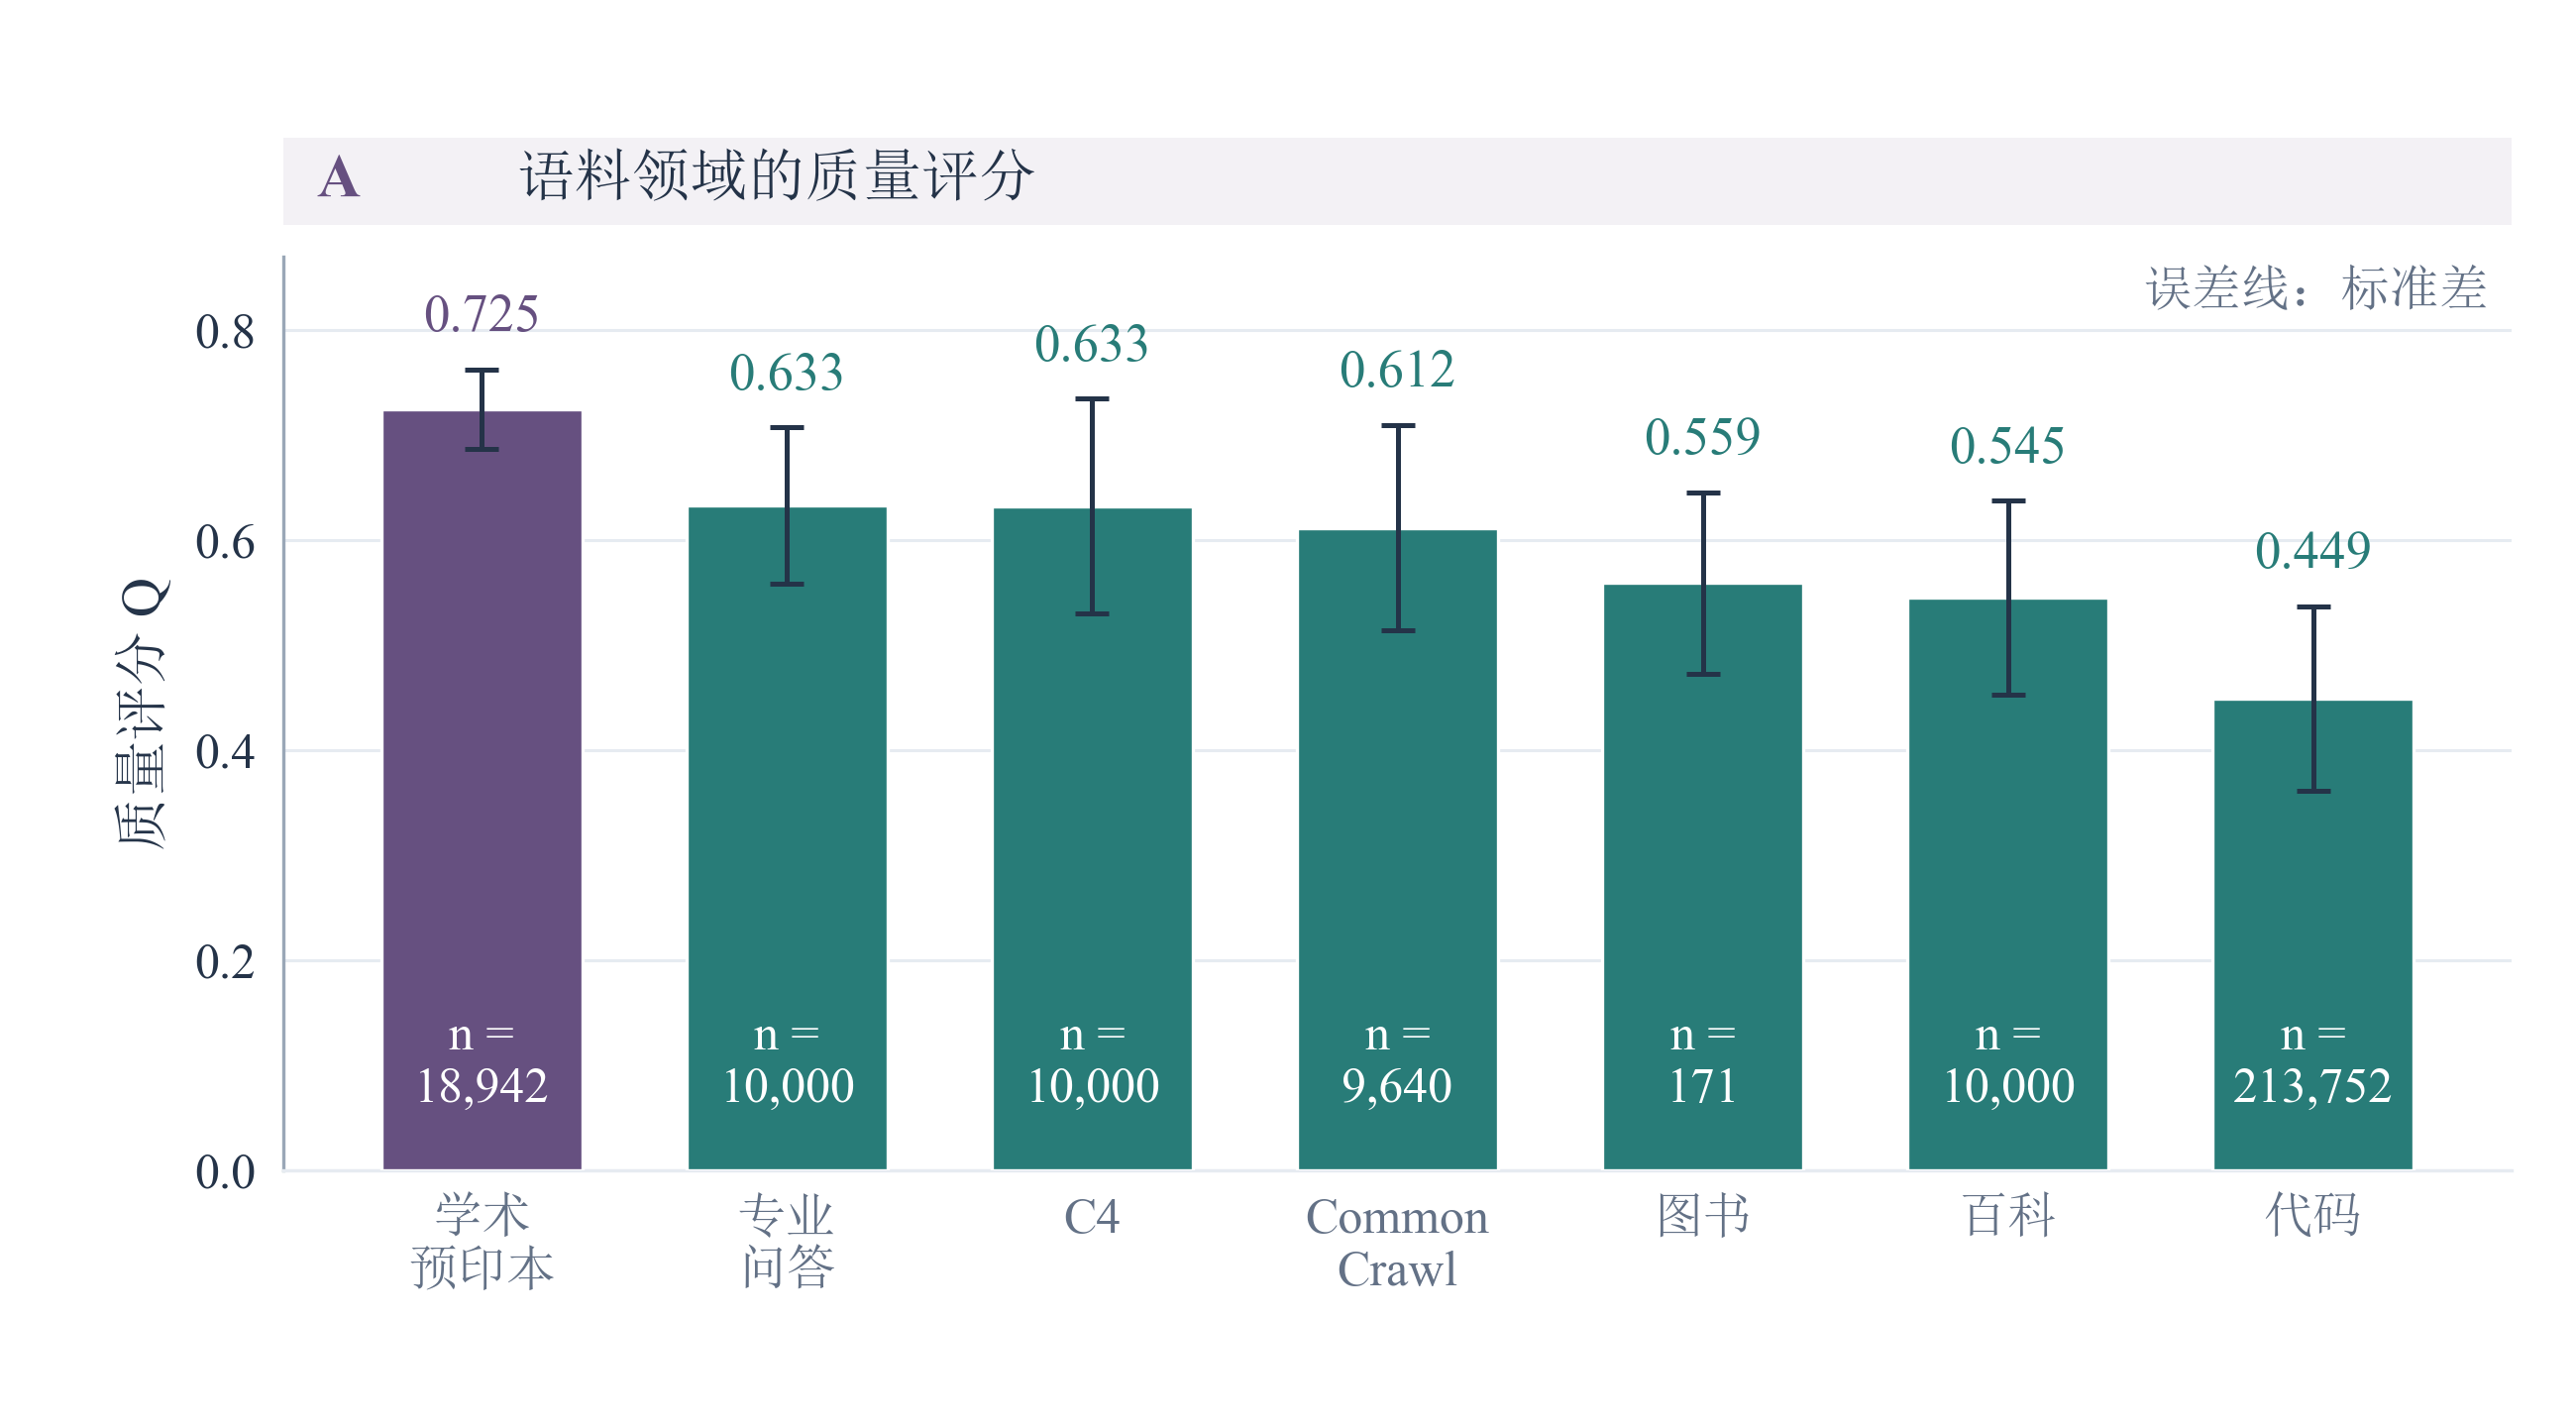
\includegraphics[width=0.62\textwidth]{../求解/问题一/图片/图0_A1-A3全量质量评分.png}
  \caption{A1--A3 全量质量信号的领域级评分（均值±标准差）}
  \label{fig:p1_quality_full}
\end{figure}

\begingroup
\setlength{\tabcolsep}{3pt}
\begin{longtable}{@{}>{\centering\arraybackslash}p{0.20\textwidth}>{\centering\arraybackslash}p{0.16\textwidth}>{\centering\arraybackslash}p{0.16\textwidth}>{\centering\arraybackslash}p{0.16\textwidth}>{\raggedright\arraybackslash}p{0.24\textwidth}@{}}
  \caption{各领域在 A1 抽样集与 A2/A3 扩展集中的质量评分}
  \label{tab:p1_qa} \\
  \toprule
  质量信号领域 & A1 评分 $Q$ & 扩展集评分 $Q$ & 评分差值 & 训练配方对应领域 \\
  \midrule
  \endfirsthead
  \caption{各领域在 A1 抽样集与 A2/A3 扩展集中的质量评分（续）} \\
  \toprule
  质量信号领域 & A1 评分 $Q$ & 扩展集评分 $Q$ & 评分差值 & 训练配方对应领域 \\
  \midrule
  \endhead
  \bottomrule
  \endfoot
  arxiv & 0.7031 & 0.7011 & $+0.0021$ & arxiv \\
  stackexchange & 0.6549 & — & — & stackexchange \\
  c4 & 0.6368 & — & — & （配方侧无同名列） \\
  commoncrawl & 0.6153 & — & — & pile\_\allowbreak{}cc \\
  book & 0.5524 & — & — & gutenberg\_\allowbreak{}pg\_\allowbreak{}19 \\
  wikipedia & 0.5509 & — & — & wikipedia\_\allowbreak{}en \\
  github & 0.4553 & 0.4547 & $+0.0006$ & github \\
\end{longtable}
\endgroup

arxiv 和 github 同时具有抽样与扩展记录，可以直接比较。表\ref{tab:p1_qa}中，两者的评分差分别为 $+0.0021$、$+0.0006$，均接近零。这说明在这两个可比较领域，抽样集和扩展集得到的平均质量较为接近。

全量评分依次为 arxiv（0.703）$>$ stackexchange（0.655）$>$ c4（0.637）$>$ commoncrawl（0.615）$>$ book（0.552）$\approx$ wikipedia（0.551）$>$ github（0.455）。该次序取决于所用的 22 个分类器信号。例如，rps\_\allowbreak{}doc\_\allowbreak{}frac\_\allowbreak{}unique\_\allowbreak{}words 和 rps\_\allowbreak{}doc\_\allowbreak{}unigram\_\allowbreak{}entropy 还会受到文档长度影响。因此，c4、commoncrawl 的评分高于 book、wikipedia，只能说明它们在本评价体系中的得分较高，不能据此判断所有训练任务中的语料价值。

表\ref{tab:p1_conf}比较各集合的冲突比例和排序一致性；图\ref{fig:p1_conf}则给出分歧较多的指标对及对应的熵权分布。

\begingroup
\setlength{\tabcolsep}{3pt}
\begin{longtable}{@{}>{\centering\arraybackslash}p{0.18\textwidth}>{\centering\arraybackslash}p{0.13\textwidth}>{\centering\arraybackslash}p{0.13\textwidth}>{\centering\arraybackslash}p{0.13\textwidth}>{\centering\arraybackslash}p{0.14\textwidth}>{\raggedright\arraybackslash}p{0.20\textwidth}@{}}
  \caption{各数据集的指标冲突比例与排序一致性}
  \label{tab:p1_conf} \\
  \toprule
  统计范围 & 记录数 & Kendall $W$ & 冲突比例 $\rho_c$ & 独立基准 $\rho_0$ & $\rho_c/\rho_0$ \\
  \midrule
  \endfirsthead
  \caption{各数据集的指标冲突比例与排序一致性（续）} \\
  \toprule
  统计范围 & 记录数 & Kendall $W$ & 冲突比例 $\rho_c$ & 独立基准 $\rho_0$ & $\rho_c/\rho_0$ \\
  \midrule
  \endhead
  \bottomrule
  \endfoot
  A1 抽样集 & 51{,}230 & 0.0783 & 0.2252 & 0.2888 & 0.780 \\
  A2+A3 扩展集 & 221{,}275 & 0.0628 & 0.2208 & 0.2888 & 0.764 \\
  全量 & 272{,}505 & 0.0687 & 0.2235 & 0.2888 & 0.774 \\
\end{longtable}
\endgroup

\begin{figure}[ht]
  \centering
  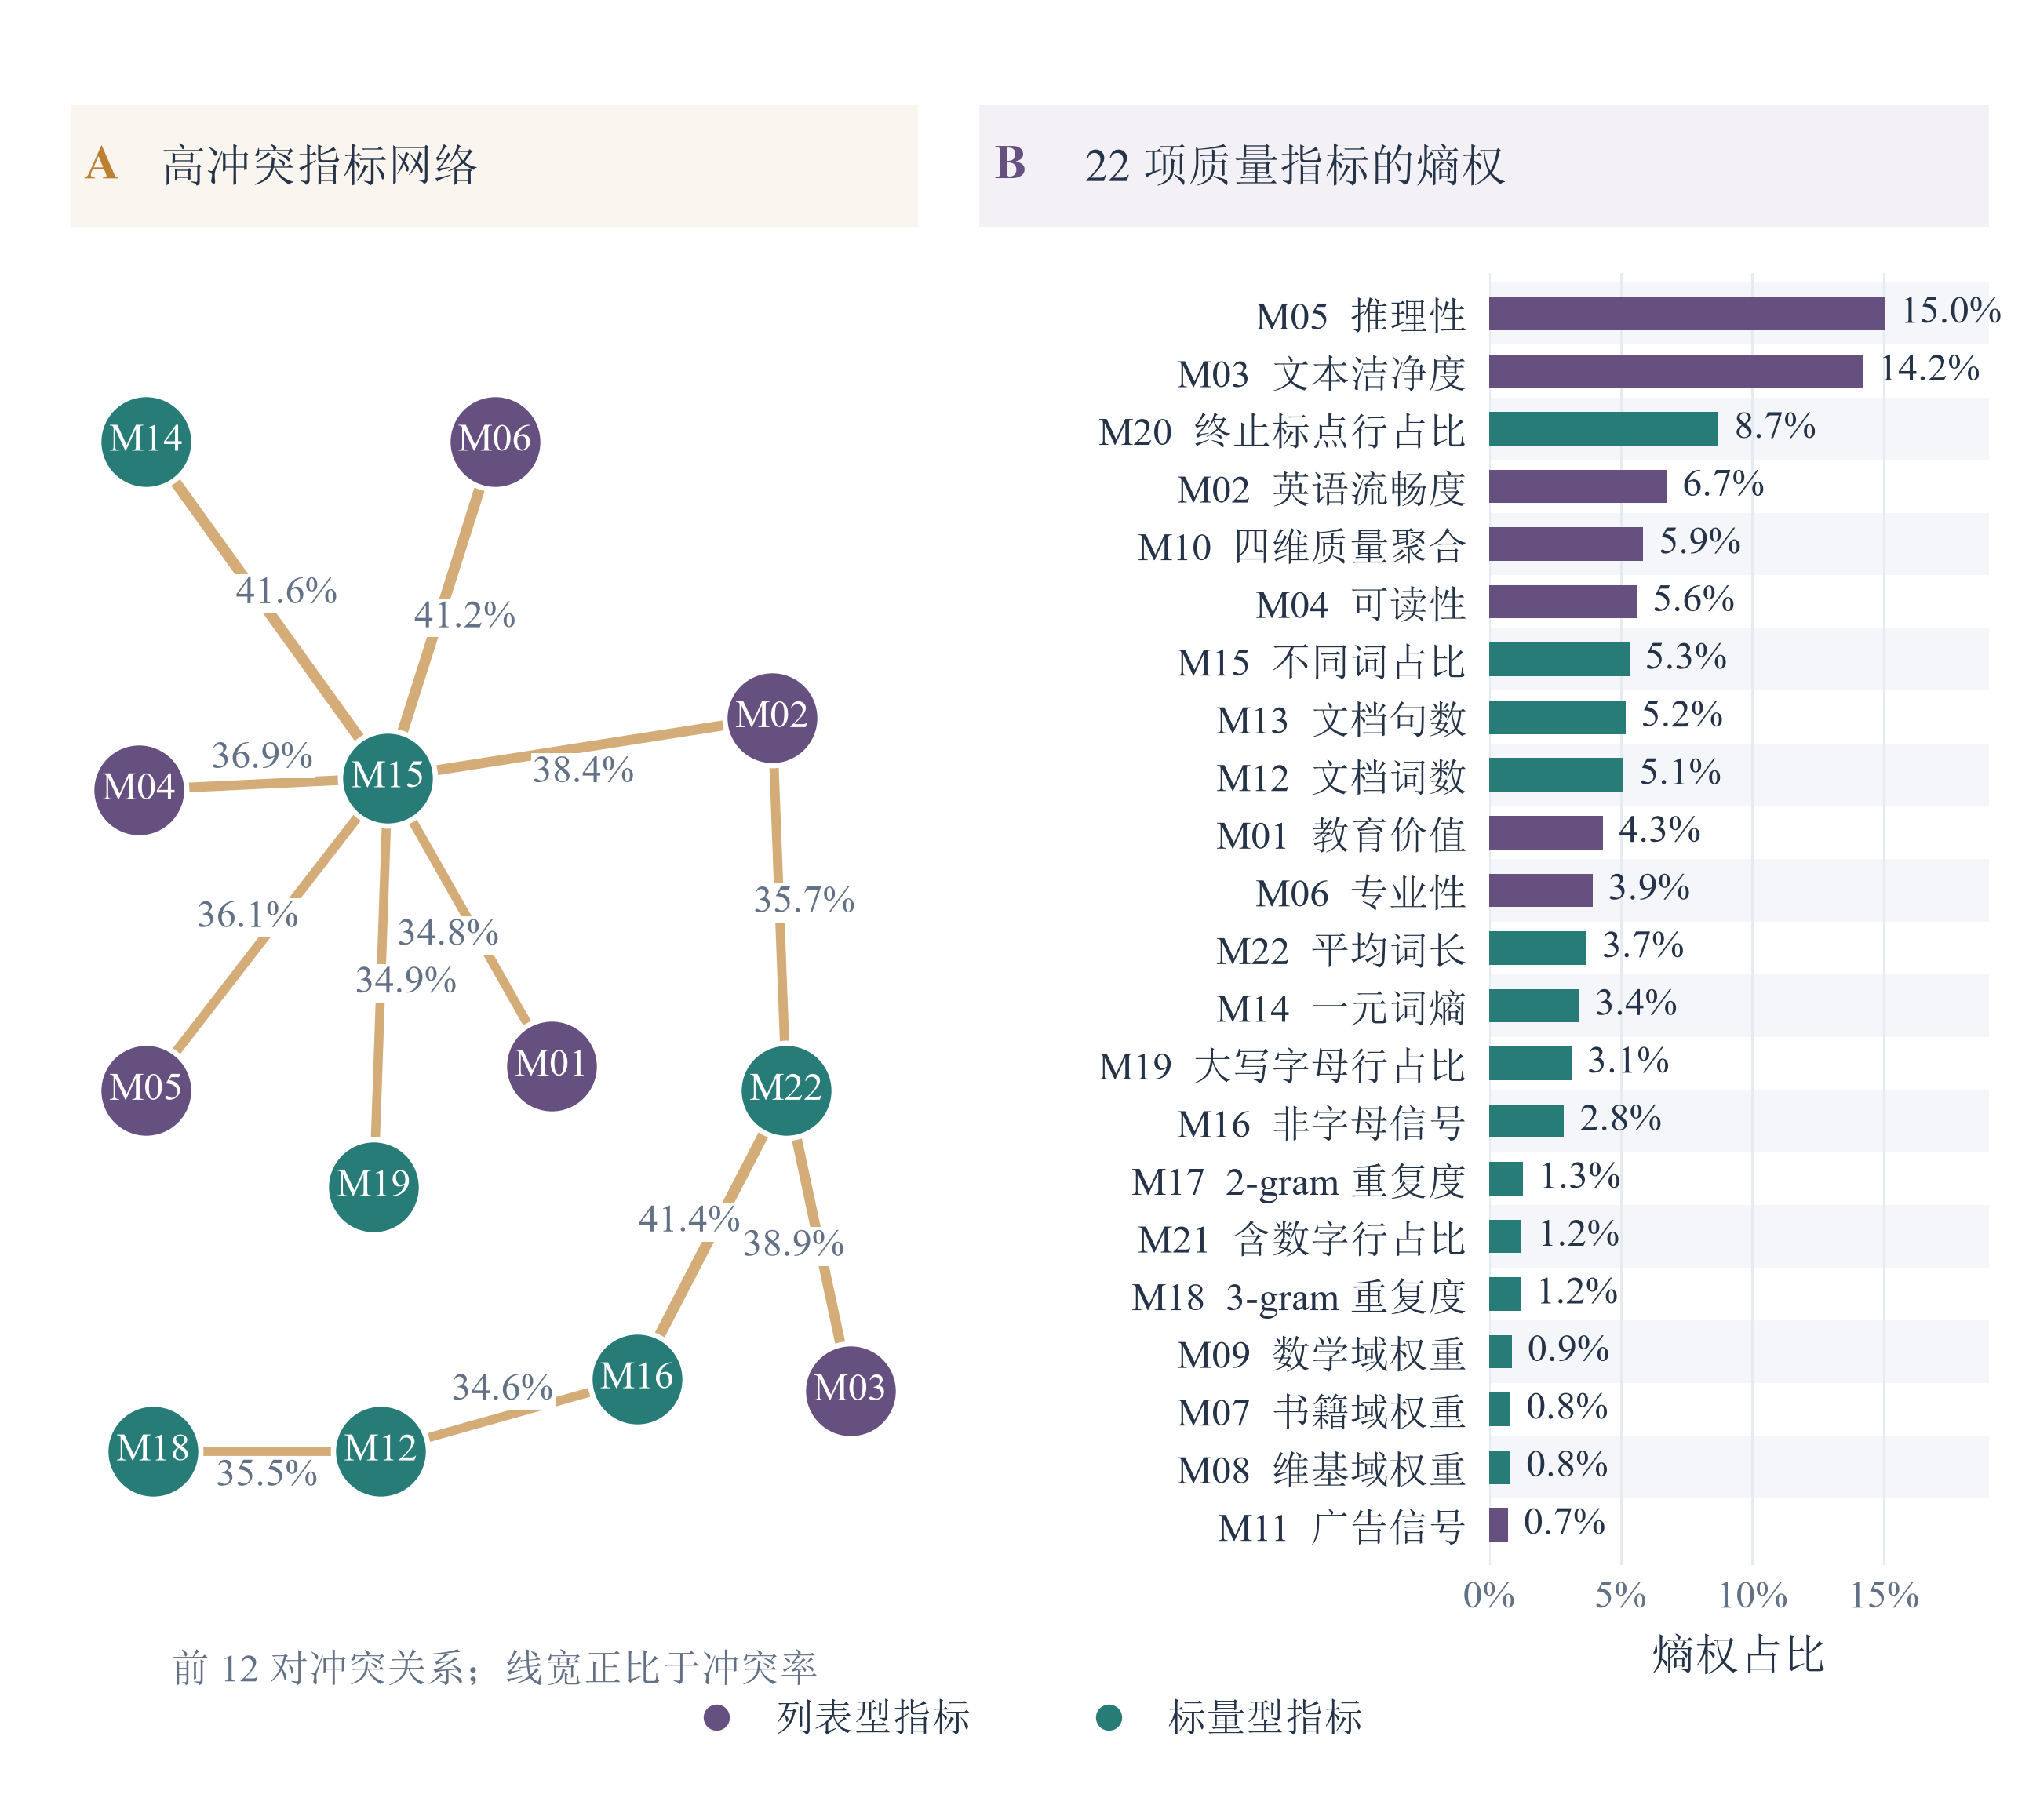
\includegraphics[width=0.92\textwidth]{../求解/问题一/图片/图6_冲突与赋权诊断.png}
  \caption{冲突最集中的指标对（左）与熵权分布（右）}
  \label{fig:p1_conf}
\end{figure}

表\ref{tab:p1_conf}中，抽样集、扩展集和全量记录的冲突率都在 $0.221\sim0.225$ 之间，表明更换统计集合后，冲突比例变化较小。

全量 Kendall 系数为 $0.069$，说明指标排序的一致程度较弱。虽然 $\chi^2$ 检验得到 $p<0.001$，但样本量很大，统计显著并不等于高度一致。同时，$22.3\%$ 的冲突率低于独立参照的 $28.9\%$，比值为 $0.774$。两项结果合起来看，各指标存在共同倾向，但仍保留较多评价分歧。

结合字段含义，可从三方面理解这些分歧。首先，指标的具体测量方式不同，如 rps\_\allowbreak{}doc\_\allowbreak{}unigram\_\allowbreak{}entropy 与 rps\_\allowbreak{}doc\_\allowbreak{}frac\_\allowbreak{}unique\_\allowbreak{}words 虽都涉及词汇多样性，计算尺度却不同。其次，同一指标在不同内容上可能有不同表现，例如 modernbert\_\allowbreak{}professionalism 对学术文本和论坛文本的评价。最后，分布形态也有影响，ad\_\allowbreak{}en 的二分类概率在长文档上容易集中于两端。

处理时保留这些样本参与领域均值计算，同时按 $Q_i$ 相对领域中位数的位置作综合裁决，并保留冲突标记。问题二、三使用聚合结果，不将冲突样本单独作为分析依据。

\Needspace{4\baselineskip}
\textbf{2. 领域配比与损失的拟合及验证}\par\nopagebreak[4]

配比拟合的结果从四个角度展示：图\ref{fig:p1_structure}给出训练配方构成，图\ref{fig:p1_r2}比较训练与检验精度，图\ref{fig:p1_scatter}对照同尺度的预测和观测损失，图\ref{fig:p1_heatmap}展示不同训练领域的系数差异。

\begin{figure}[ht]
  \centering
  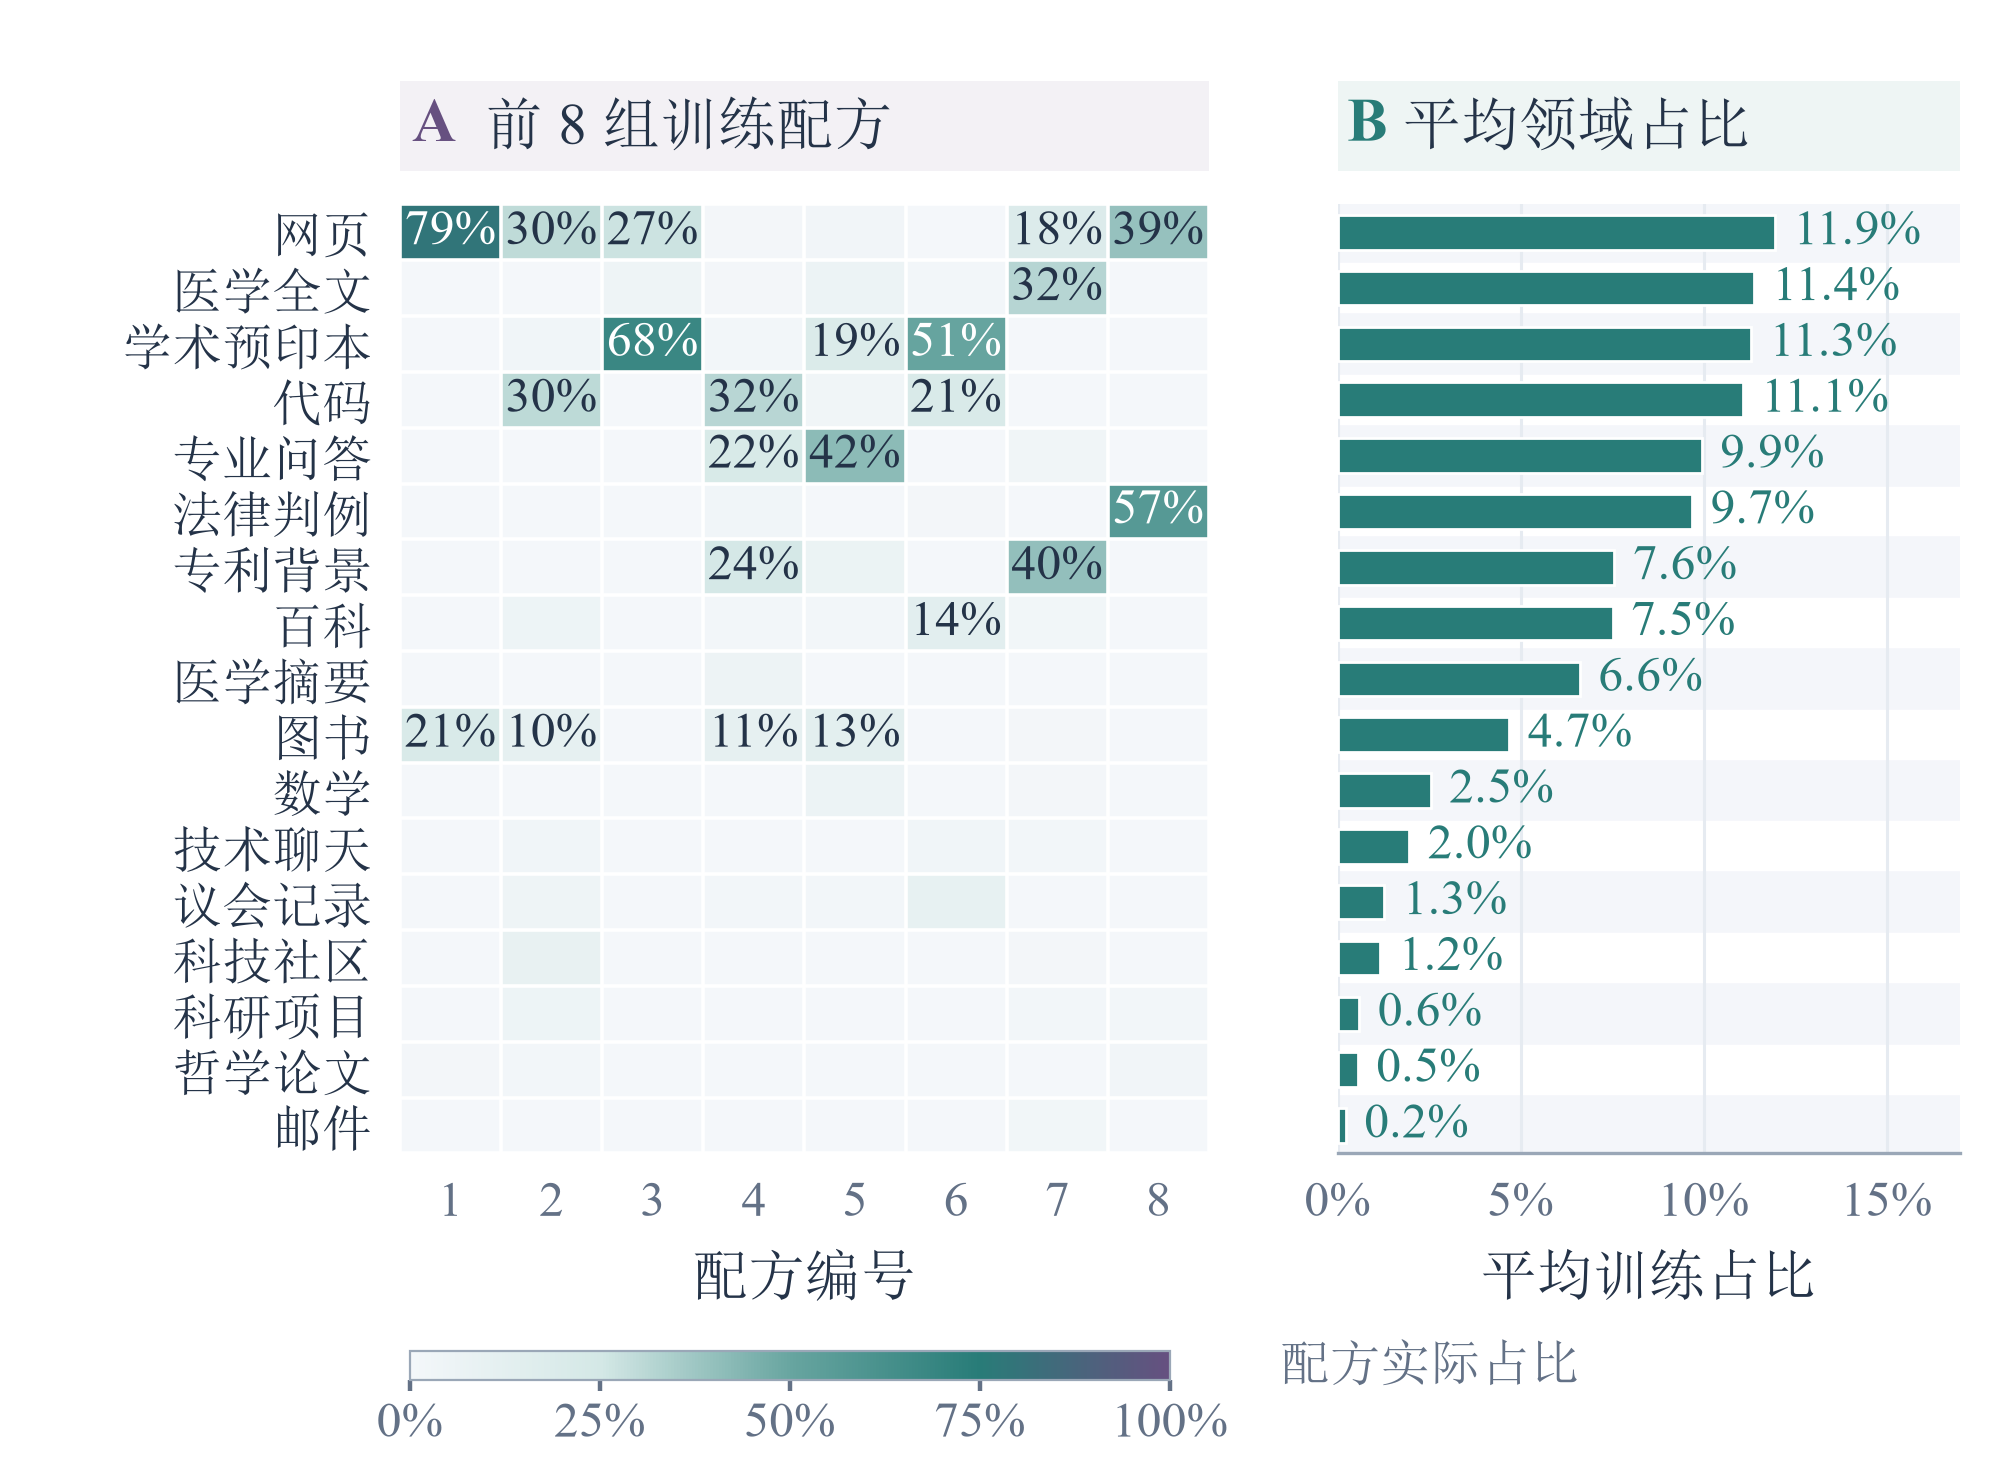
\includegraphics[width=0.92\textwidth]{../求解/问题一/图片/图1_训练配比结构.png}
  \caption{训练配方结构（左：前 8 组配方堆叠；右：全部配方平均配比）}
  \label{fig:p1_structure}
\end{figure}

\begin{figure}[ht]
  \centering
  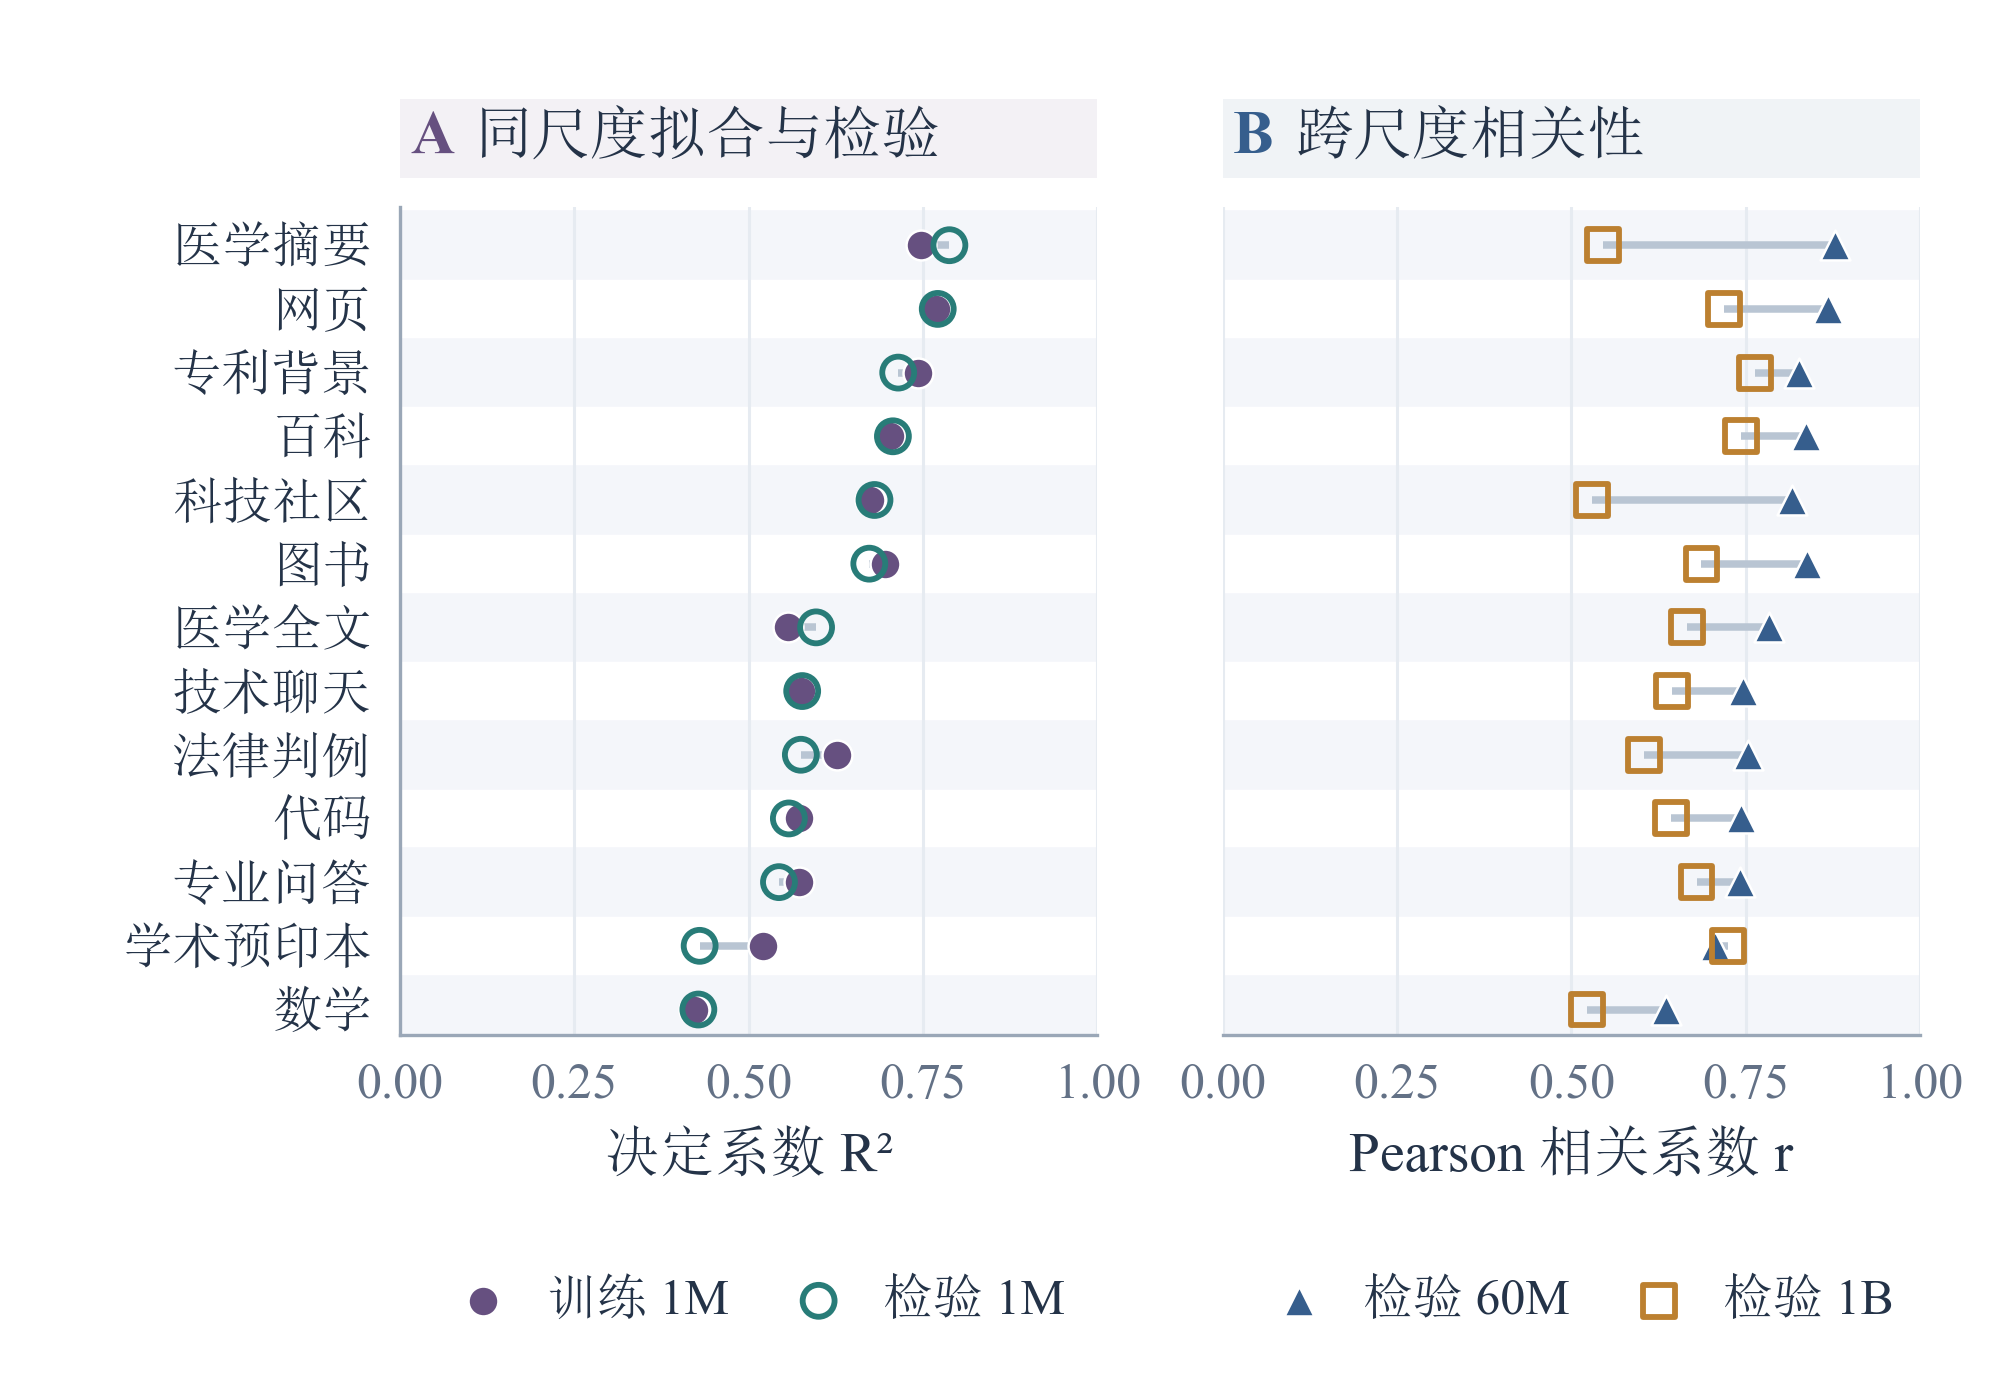
\includegraphics[width=0.72\textwidth]{../求解/问题一/图片/图2_线性模型R2.png}
  \caption{线性混合回归的拟合与泛化表现}
  \label{fig:p1_r2}
\end{figure}

\begin{figure}[ht]
  \centering
  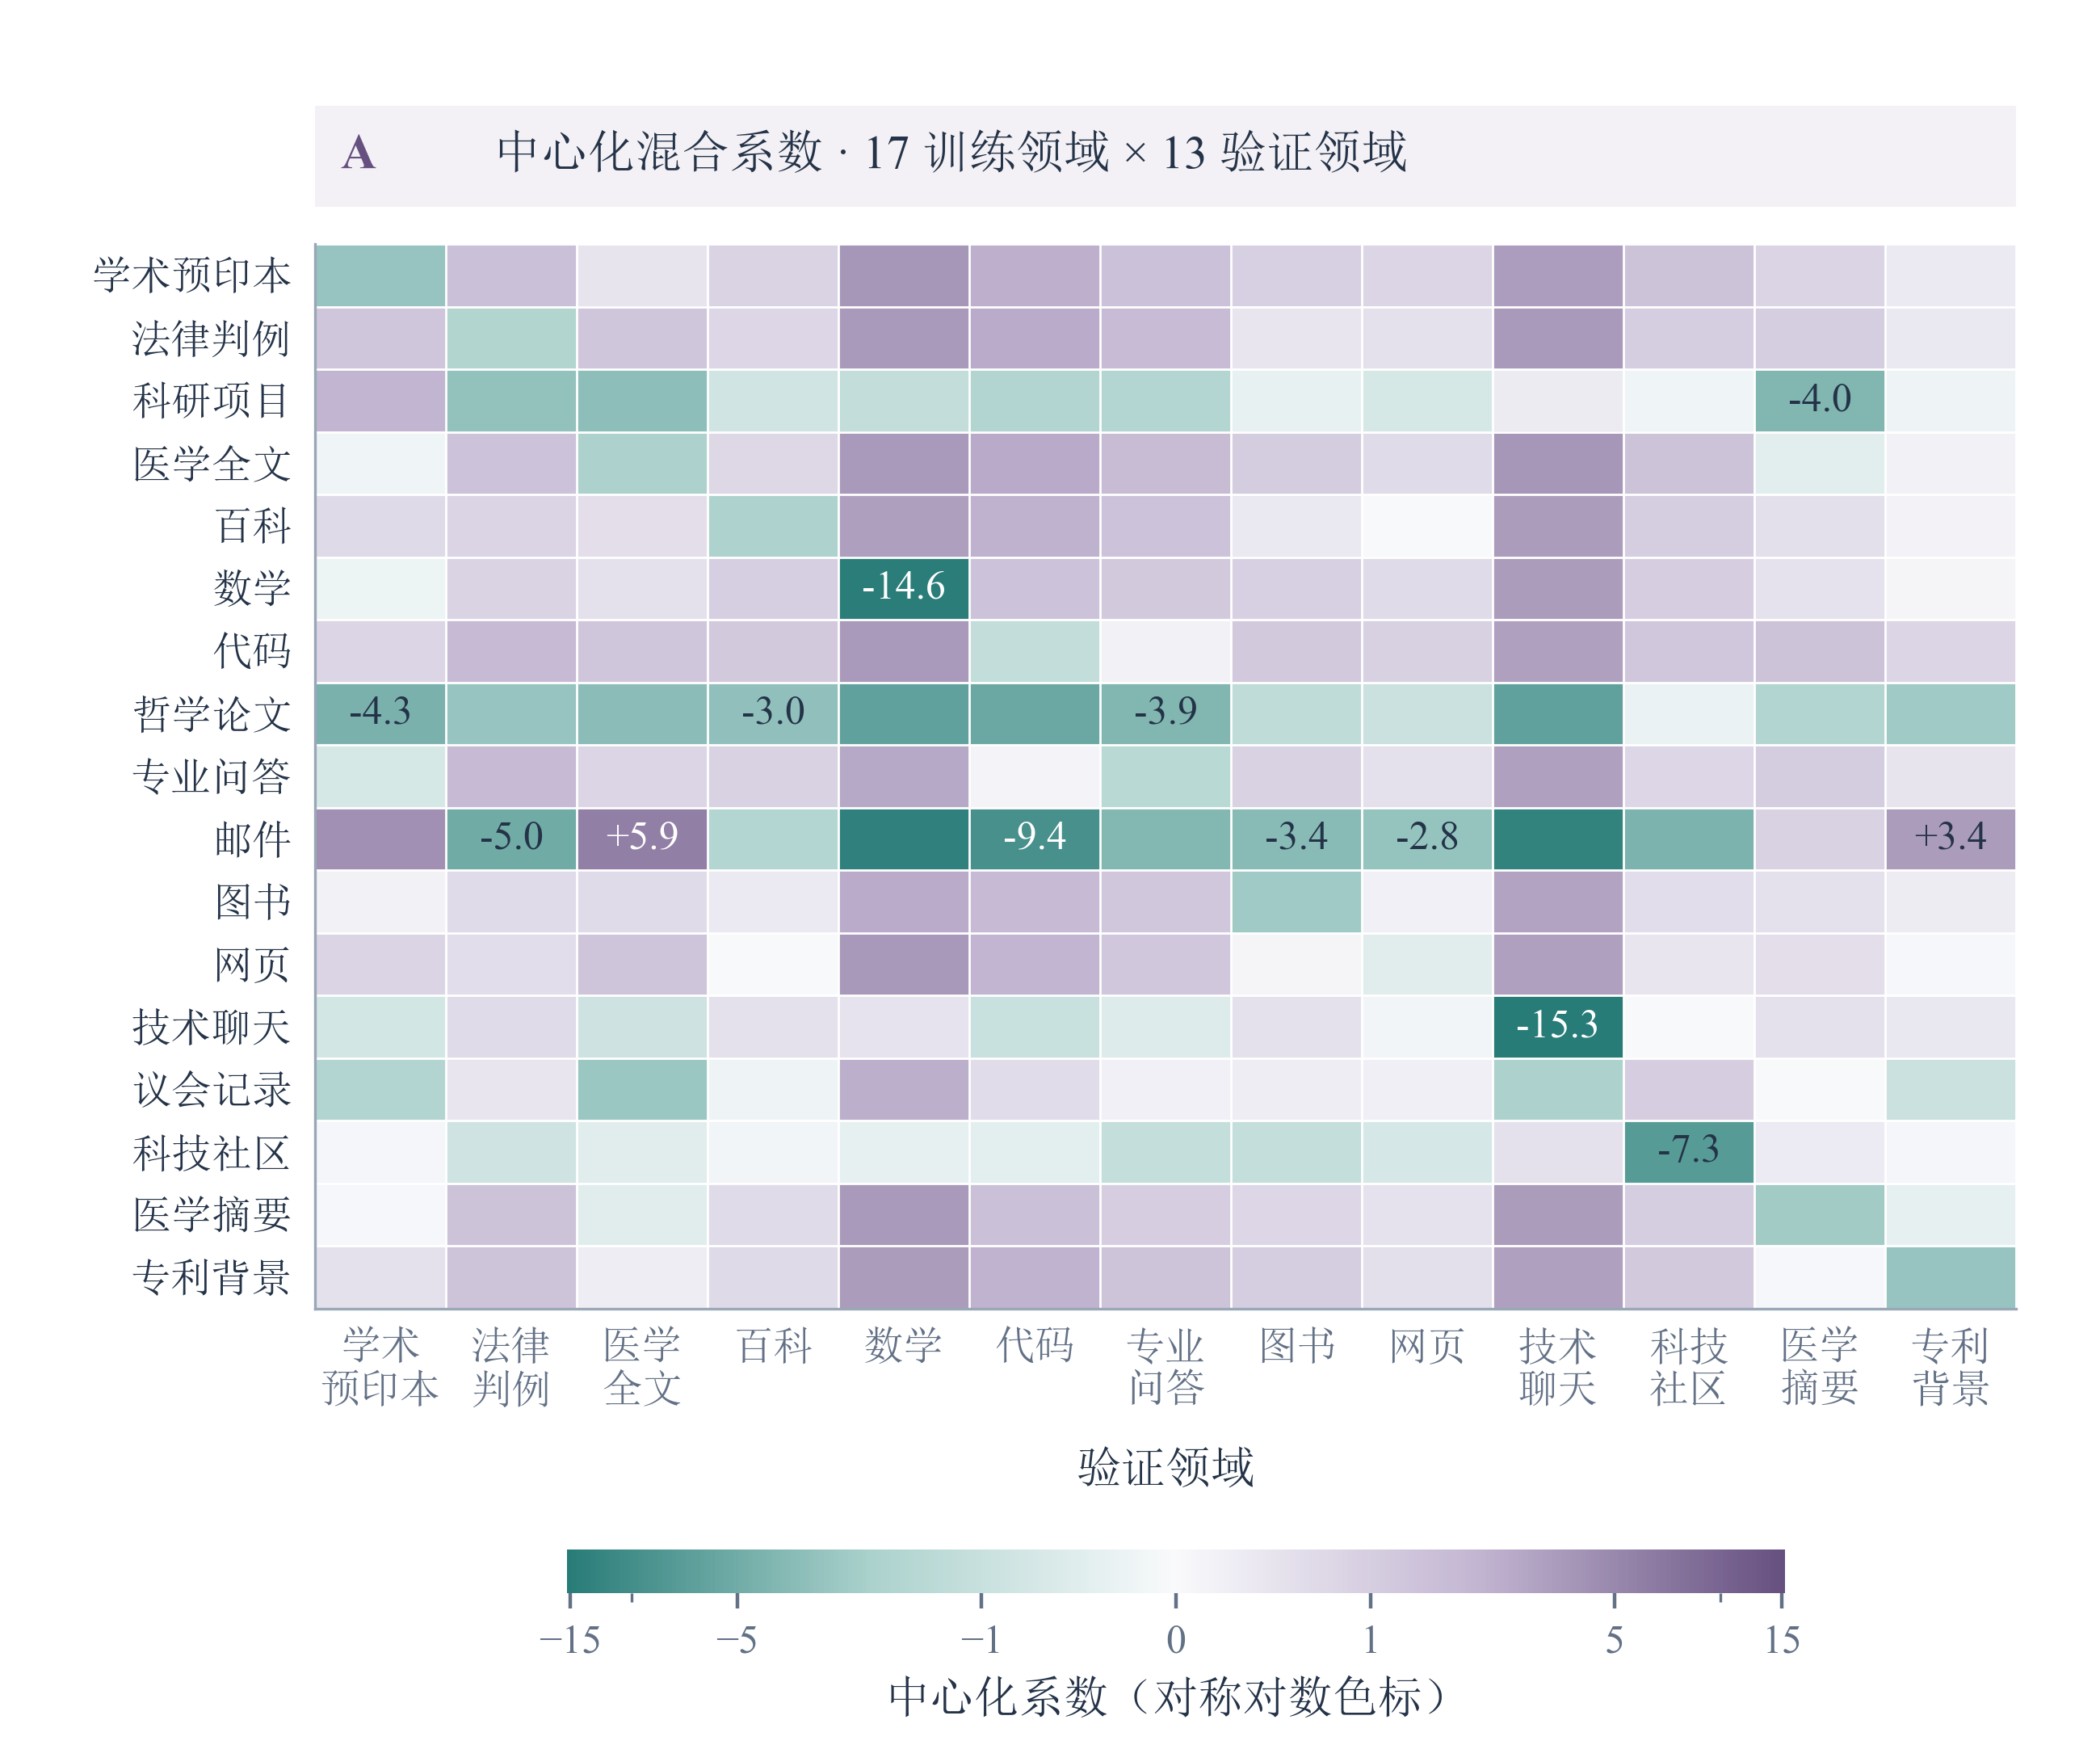
\includegraphics[width=0.78\textwidth]{../求解/问题一/图片/图4_混合系数热力图.png}
  \caption{领域配比对交叉熵损失的相对影响热力图}
  \label{fig:p1_heatmap}
\end{figure}

\begin{figure}[ht]
  \centering
  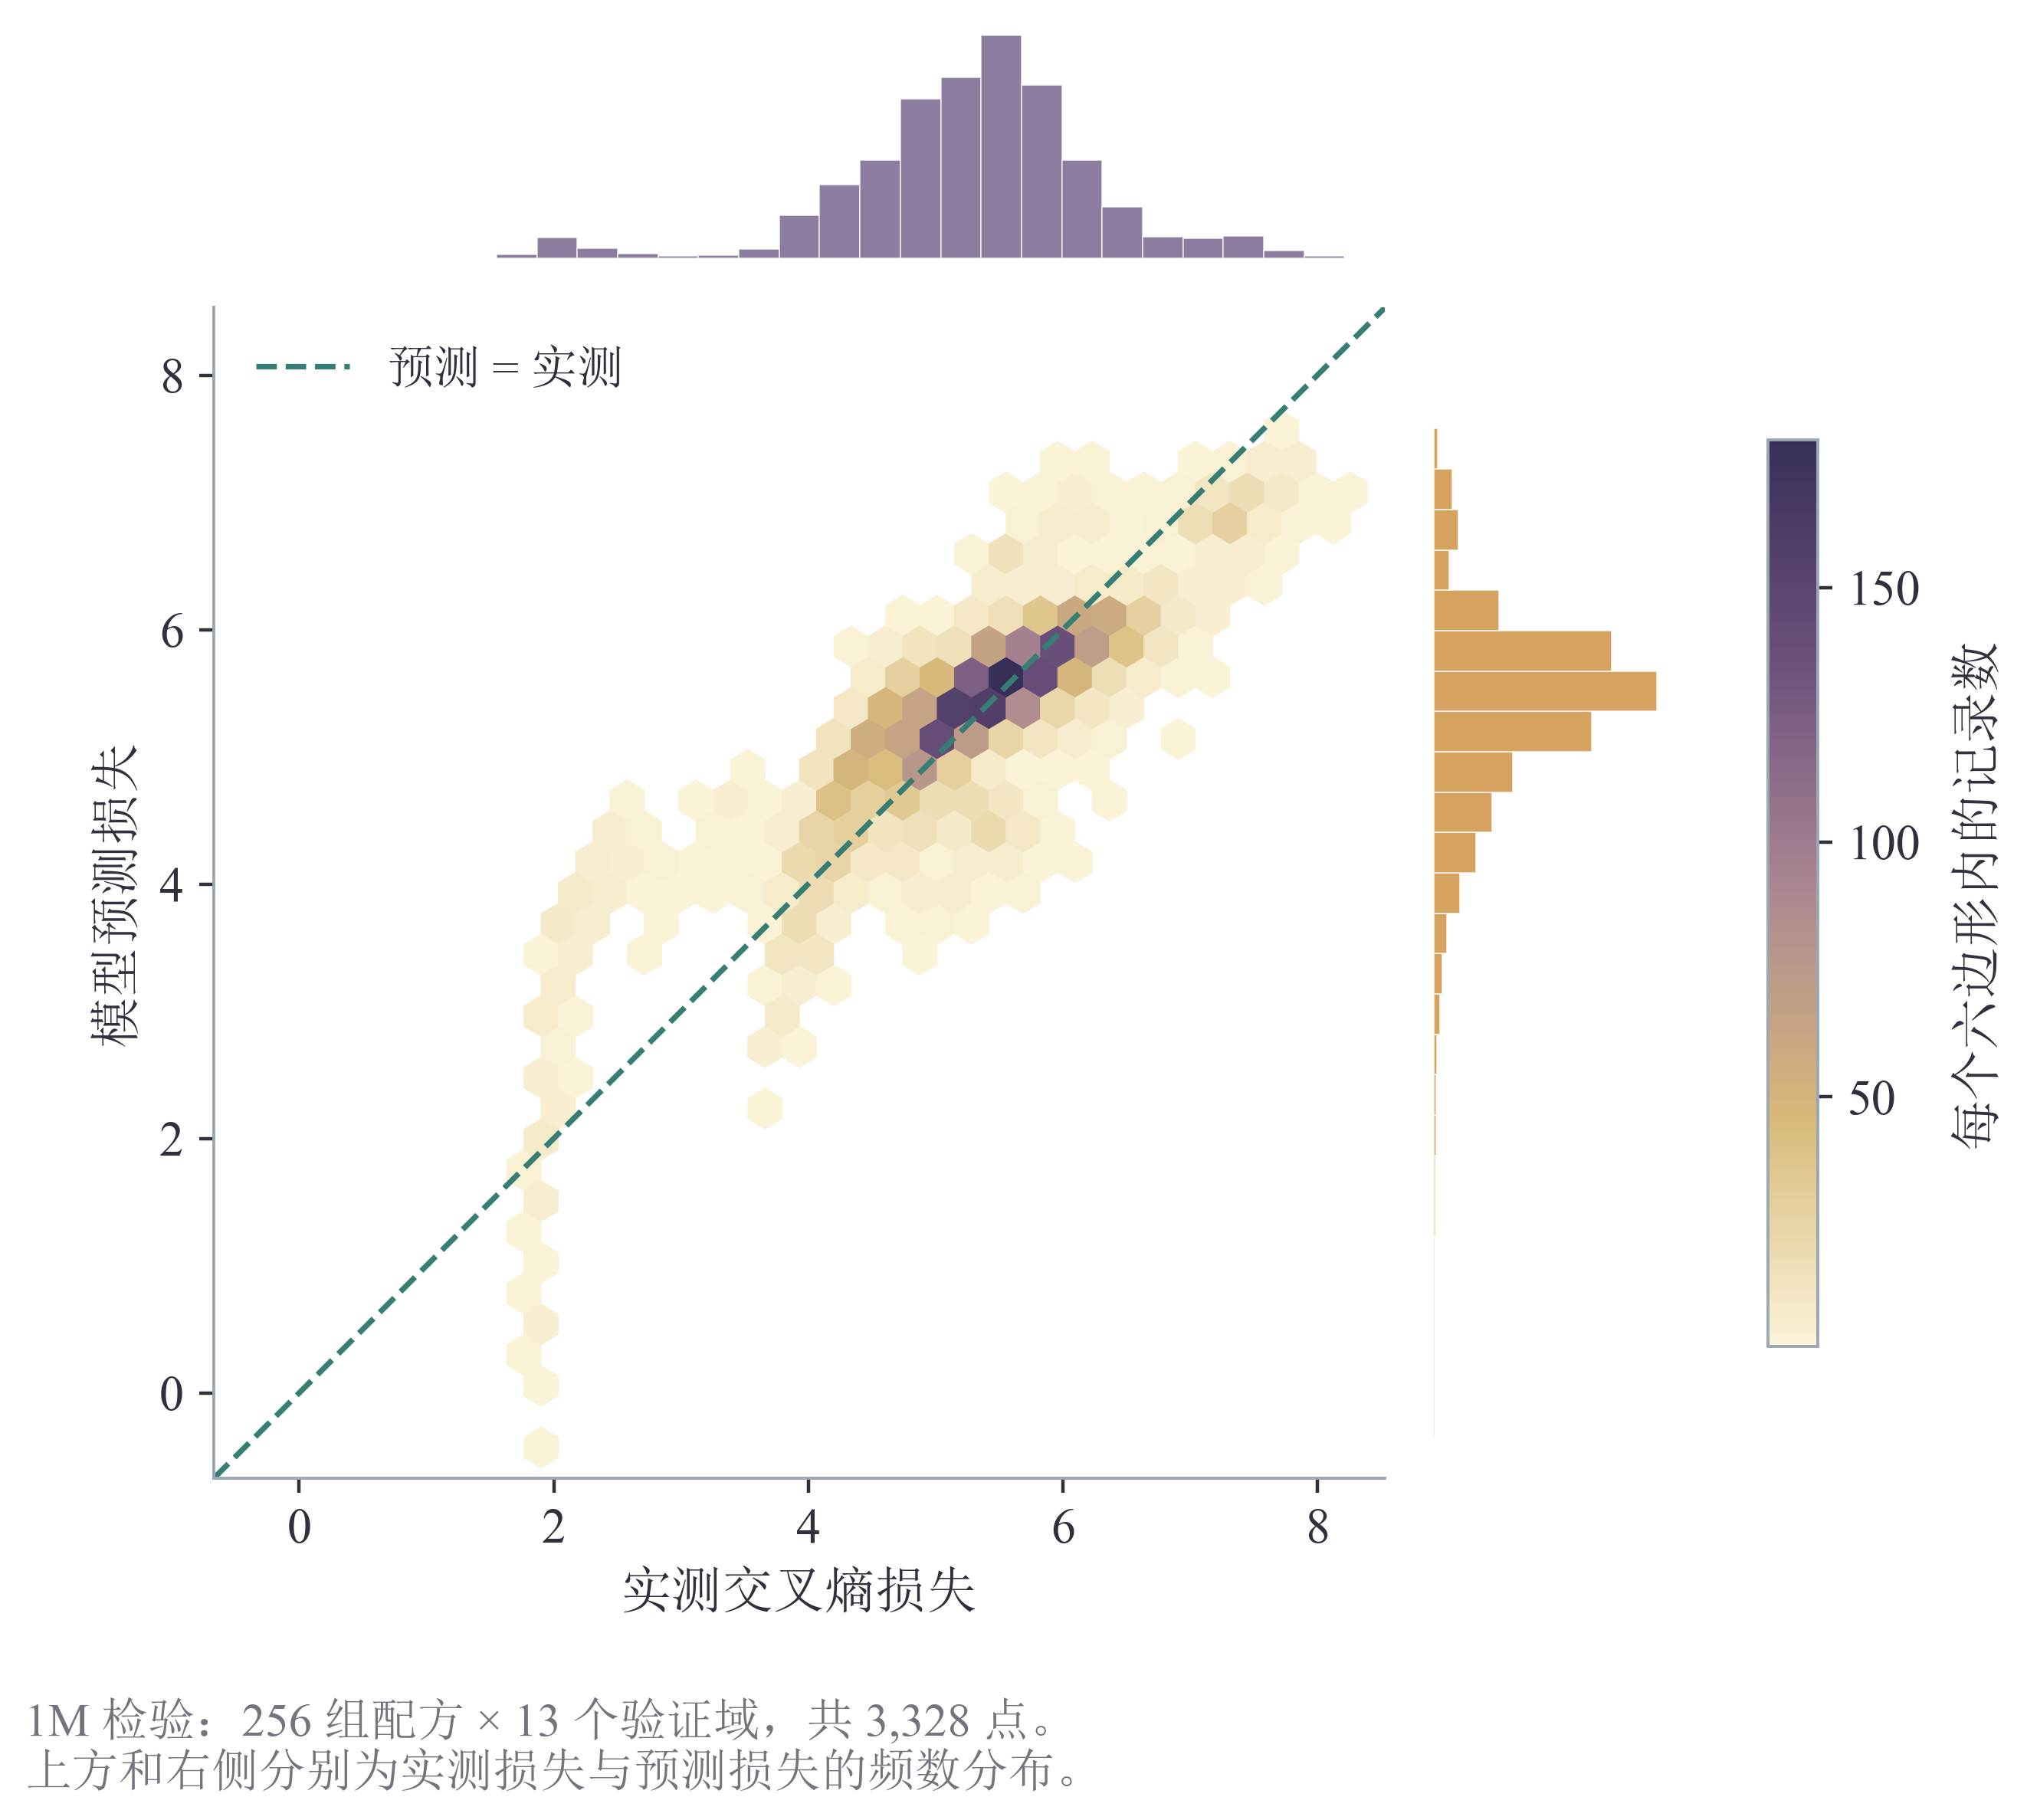
\includegraphics[width=0.58\textwidth]{../求解/问题一/图片/图3_预测vs实测.png}
  \caption{同尺度检验集（1M）预测损失与实测损失对比}
  \label{fig:p1_scatter}
\end{figure}

在图\ref{fig:p1_r2}中，13 个验证域的训练 $R^2$ 为 $0.42\sim0.77$，平均为 $0.629$。1M 同尺度检验的平均值为 $0.619$，与训练结果接近，未显示明显的训练集过拟合现象。

不同规模模型的损失基准不同，60M 与 1M 的损失比约为 $0.68$，直接沿用原损失尺度会影响误差评价。为比较变化趋势，我们补充计算 Pearson 相关：60M 和 1B 检验集的平均值分别为 $0.782$、$0.651$。这支持配比关系在跨规模时仍保留部分预测趋势，但绝对损失还需考虑尺度调整。

图\ref{fig:p1_heatmap}显示，各训练领域对验证任务的作用并不相同。dm\_\allowbreak{}mathematics、arxiv 等领域在部分任务上对应较低损失，pile\_\allowbreak{}cc、ubuntu\_\allowbreak{}irc 等领域则表现出不同方向。配比选择因而需要结合验证任务权重，不能仅看某一个系数。

在原模型中再加入混合质量指数 $\bar Q$ 后，13 个验证域的平均 $R^2$ 仅提高 $9.9\times10^{-5}$。由于 $\bar Q$ 本身由配比线性组合而成，这一结果说明它在当前模型中没有提供明显的新信息。本文因此保留原配比回归，并在问题二、三中通过附件 B 的半合成质量实验讨论质量投入。

文本质量与损失难度并非同一个概念。图\ref{fig:p1_quality}利用 6 个可映射领域，对照 A1--A3 的熵权评分 $Q$ 与损失代理 $Q^{(\text{loss})}$ 的排序。

\begin{figure}[ht]
  \centering
  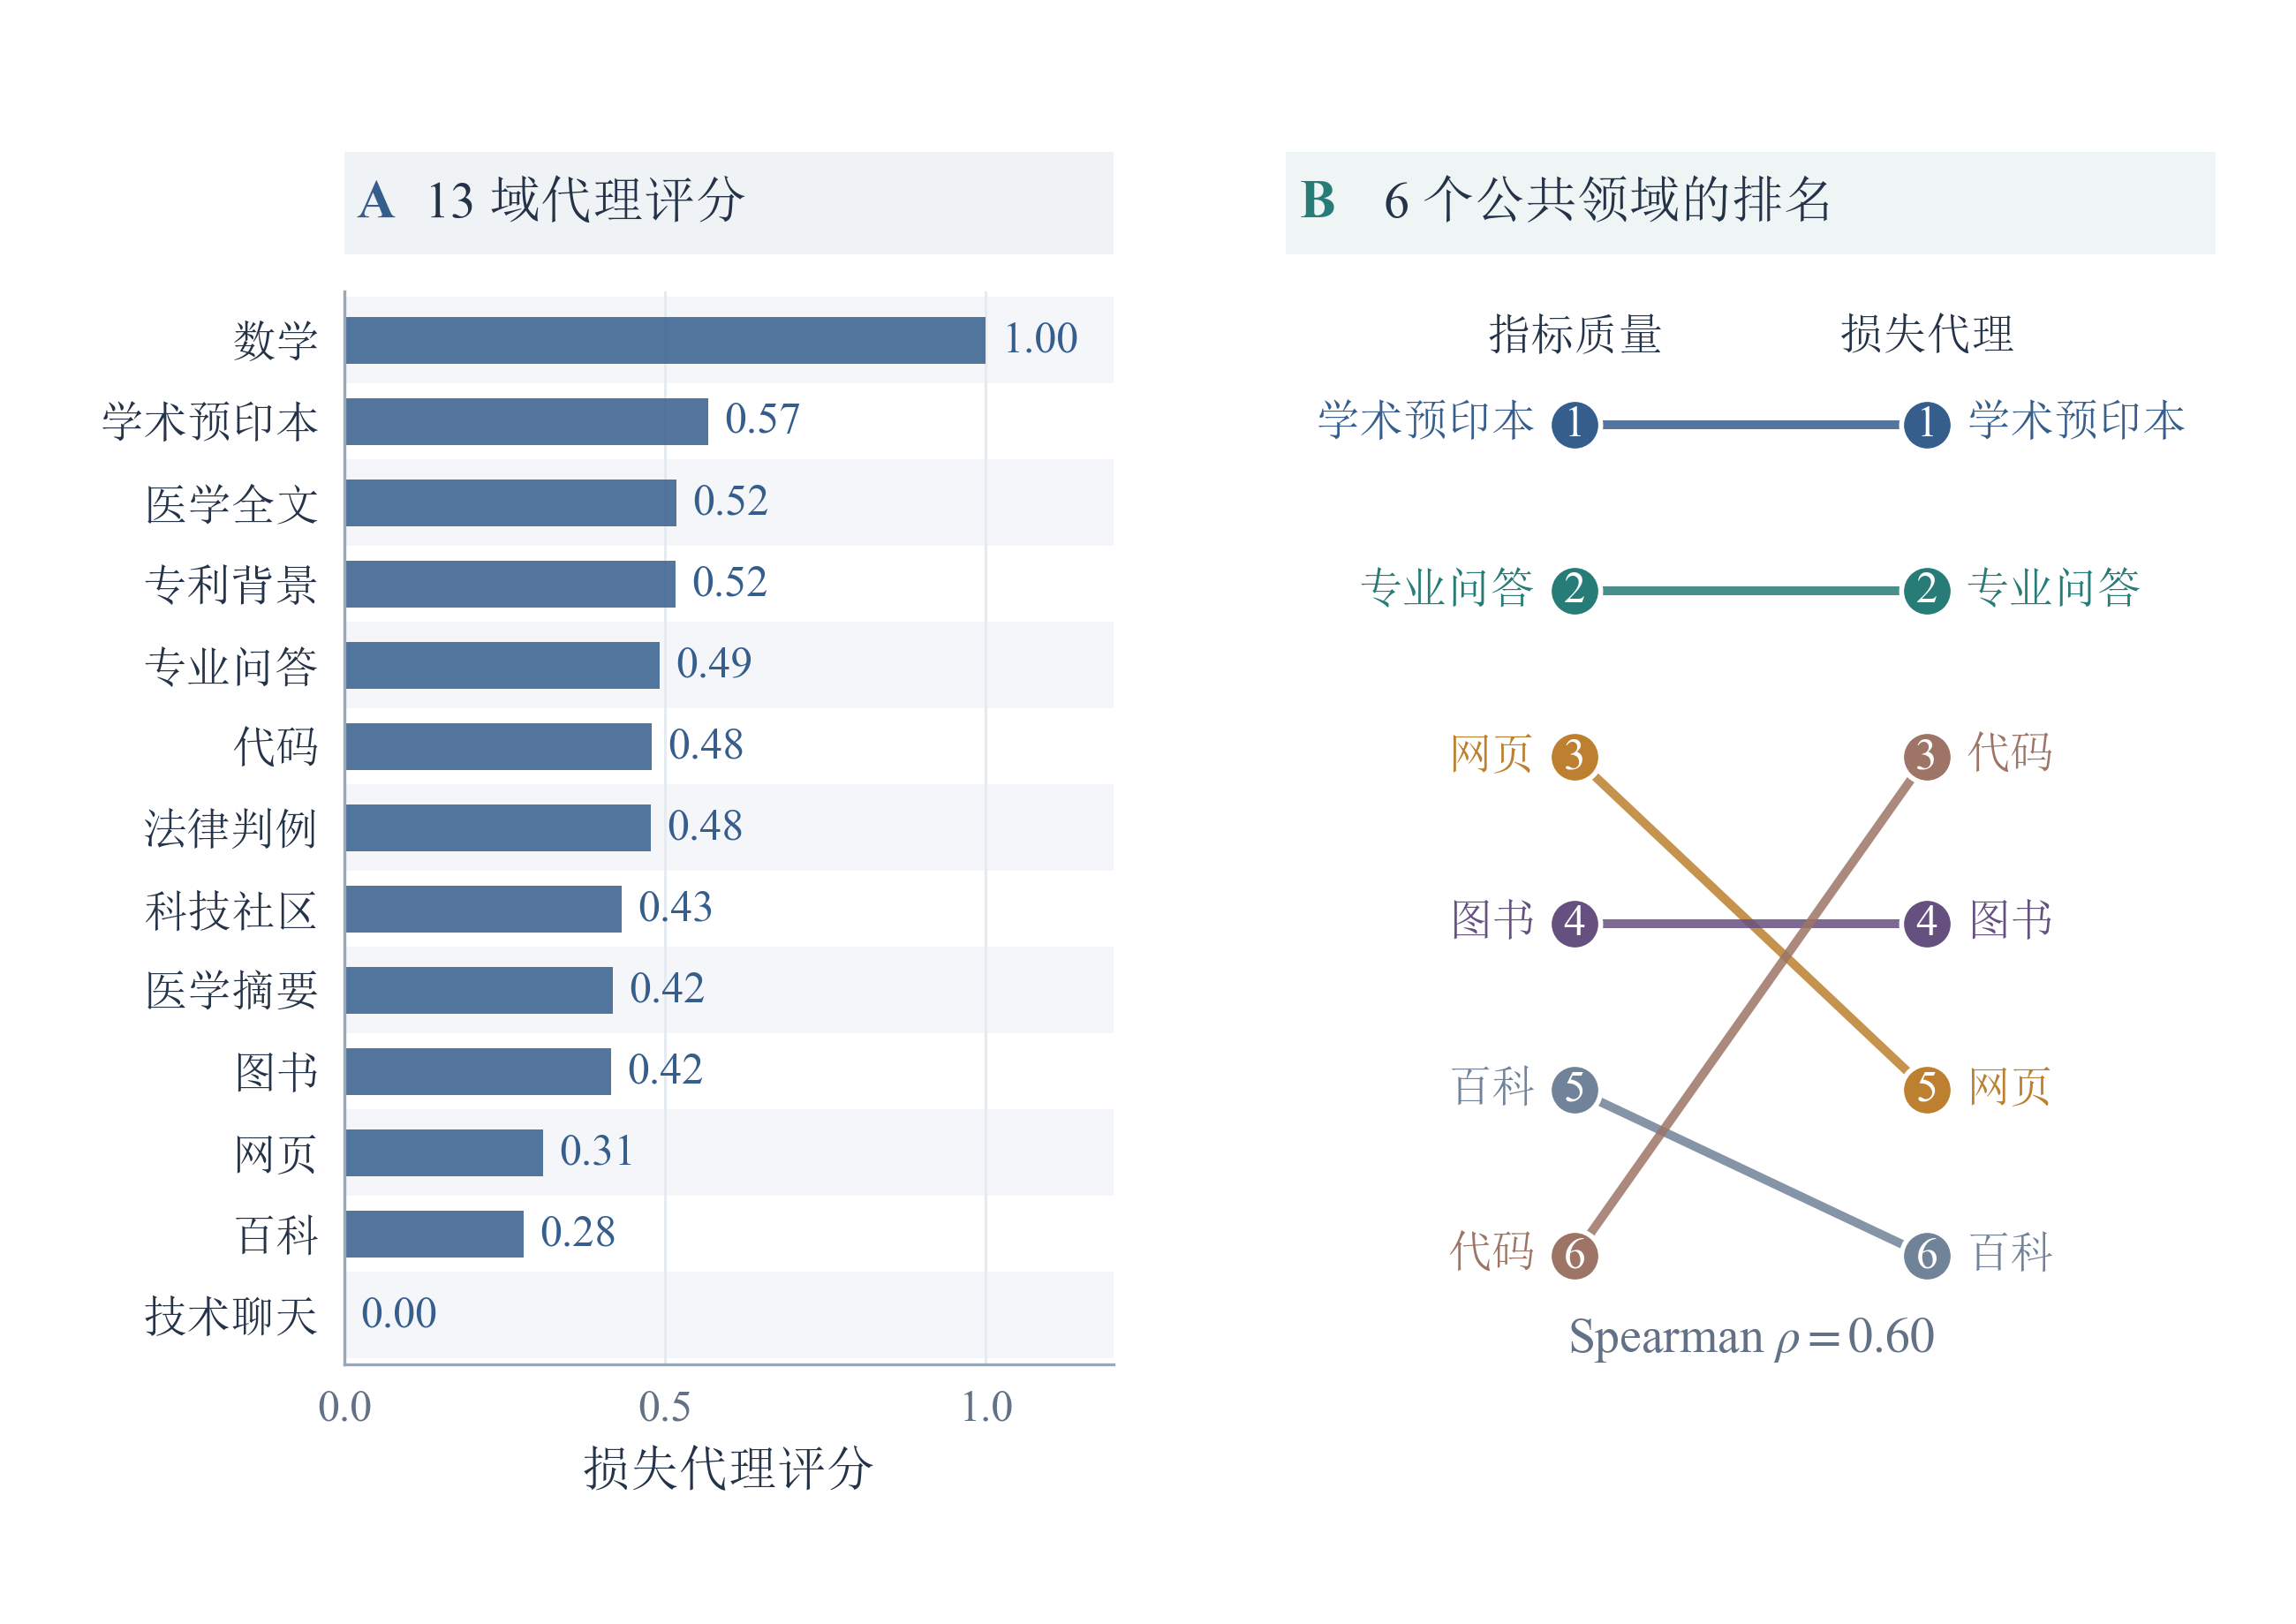
\includegraphics[width=0.92\textwidth]{../求解/问题一/图片/图5_领域质量评分.png}
  \caption{左：13 个验证域的损失难度代理；右：A1--A3 质量与损失难度代理的排序一致性}
  \label{fig:p1_quality}
\end{figure}

图\ref{fig:p1_quality}(a)比较了 13 个验证域，其中 dm\_\allowbreak{}mathematics 的代理质量为 $1.000$，ubuntu\_\allowbreak{}irc 为 $0.000$，分别对应本组验证损失的低端和高端。图\ref{fig:p1_quality}(b)所用 direct/near\_\allowbreak{}direct 映射来自 A16，两套评分的 Spearman 系数为 $0.60$。arxiv、stackexchange、github 的相对次序较一致，而 wikipedia、book、pile\_\allowbreak{}cc 存在分歧。这说明文本被评为高质量，并不保证在当前模型和验证条件下容易拟合。后续进行语料治理时采用文本质量评分，预测损失时则另行考虑领域难度。

\Needspace{4\baselineskip}
\textbf{3. 配比推荐与跨尺度分析}\par\nopagebreak[4]

若不限制各域占比上限，线性目标会将配方集中到单一低损失领域，预测加权损失为 $4.177$。为避免推荐方案过度集中，本文把上限设为参考占比的 2.5 倍。表\ref{tab:p1_rec}给出的有界方案使预测损失从 $5.336$ 降至 $5.136$，按未舍入结果计算下降 $0.199$。

\begingroup
\setlength{\tabcolsep}{3pt}
\begin{longtable}{@{}>{\centering\arraybackslash}p{0.30\textwidth}>{\centering\arraybackslash}p{0.22\textwidth}>{\centering\arraybackslash}p{0.22\textwidth}>{\centering\arraybackslash}p{0.20\textwidth}@{}}
  \caption{配比上限约束下的推荐方案与参考方案}
  \label{tab:p1_rec} \\
  \toprule
  训练领域 & 参考占比 & 推荐占比 & 占比变化量 \\
  \midrule
  \endfirsthead
  \caption{配比上限约束下的推荐方案与参考方案（续）} \\
  \toprule
  训练领域 & 参考占比 & 推荐占比 & 占比变化量 \\
  \midrule
  \endhead
  \bottomrule
  \endfoot
  pubmed\_\allowbreak{}central & 0.1137 & 0.2843 & $+0.1706$ \\
  stackexchange & 0.0994 & 0.2486 & $+0.1491$ \\
  pubmed\_\allowbreak{}abstracts & 0.0662 & 0.1654 & $+0.0993$ \\
  gutenberg\_\allowbreak{}pg\_\allowbreak{}19 & 0.0469 & 0.1173 & $+0.0704$ \\
  dm\_\allowbreak{}mathematics & 0.0255 & 0.0637 & $+0.0382$ \\
  uspto\_\allowbreak{}backgrounds & 0.0755 & 0.0000 & $-0.0755$ \\
  freelaw & 0.0968 & 0.0000 & $-0.0968$ \\
  github & 0.1107 & 0.0000 & $-0.1107$ \\
  arxiv & 0.1130 & 0.0000 & $-0.1130$ \\
  pile\_\allowbreak{}cc & 0.1195 & 0.0000 & $-0.1195$ \\
\end{longtable}
\endgroup

表\ref{tab:p1_rec}中，pubmed\_\allowbreak{}central、stackexchange、pubmed\_\allowbreak{}abstracts 的推荐占比增加，pile\_\allowbreak{}cc、arxiv、github、freelaw 的占比下降。这里优化的是 13 个验证域的加权平均损失，因此结果不等同于各领域自身表现的优劣。例如，arxiv 的占比降低只表示在当前权重和约束下，其他分配更有利于总体目标，不能解释为该领域文本质量低。

图\ref{fig:p1_extrap}进一步比较规模变化后的损失比例。10B 外推表的 est/train 因子均值为 $0.338$、标准差为 $0.038$，70B 对应 $0.266$ 和 $0.036$；同配方下，各域 60M/1M 损失比的均值为 $0.51\sim0.82$。这些比例可作为调整跨规模预测的参照，其中 10B、70B 本身属于外推记录，只能用于检查估算关系的一致性。

\begin{figure}[H]
  \centering
  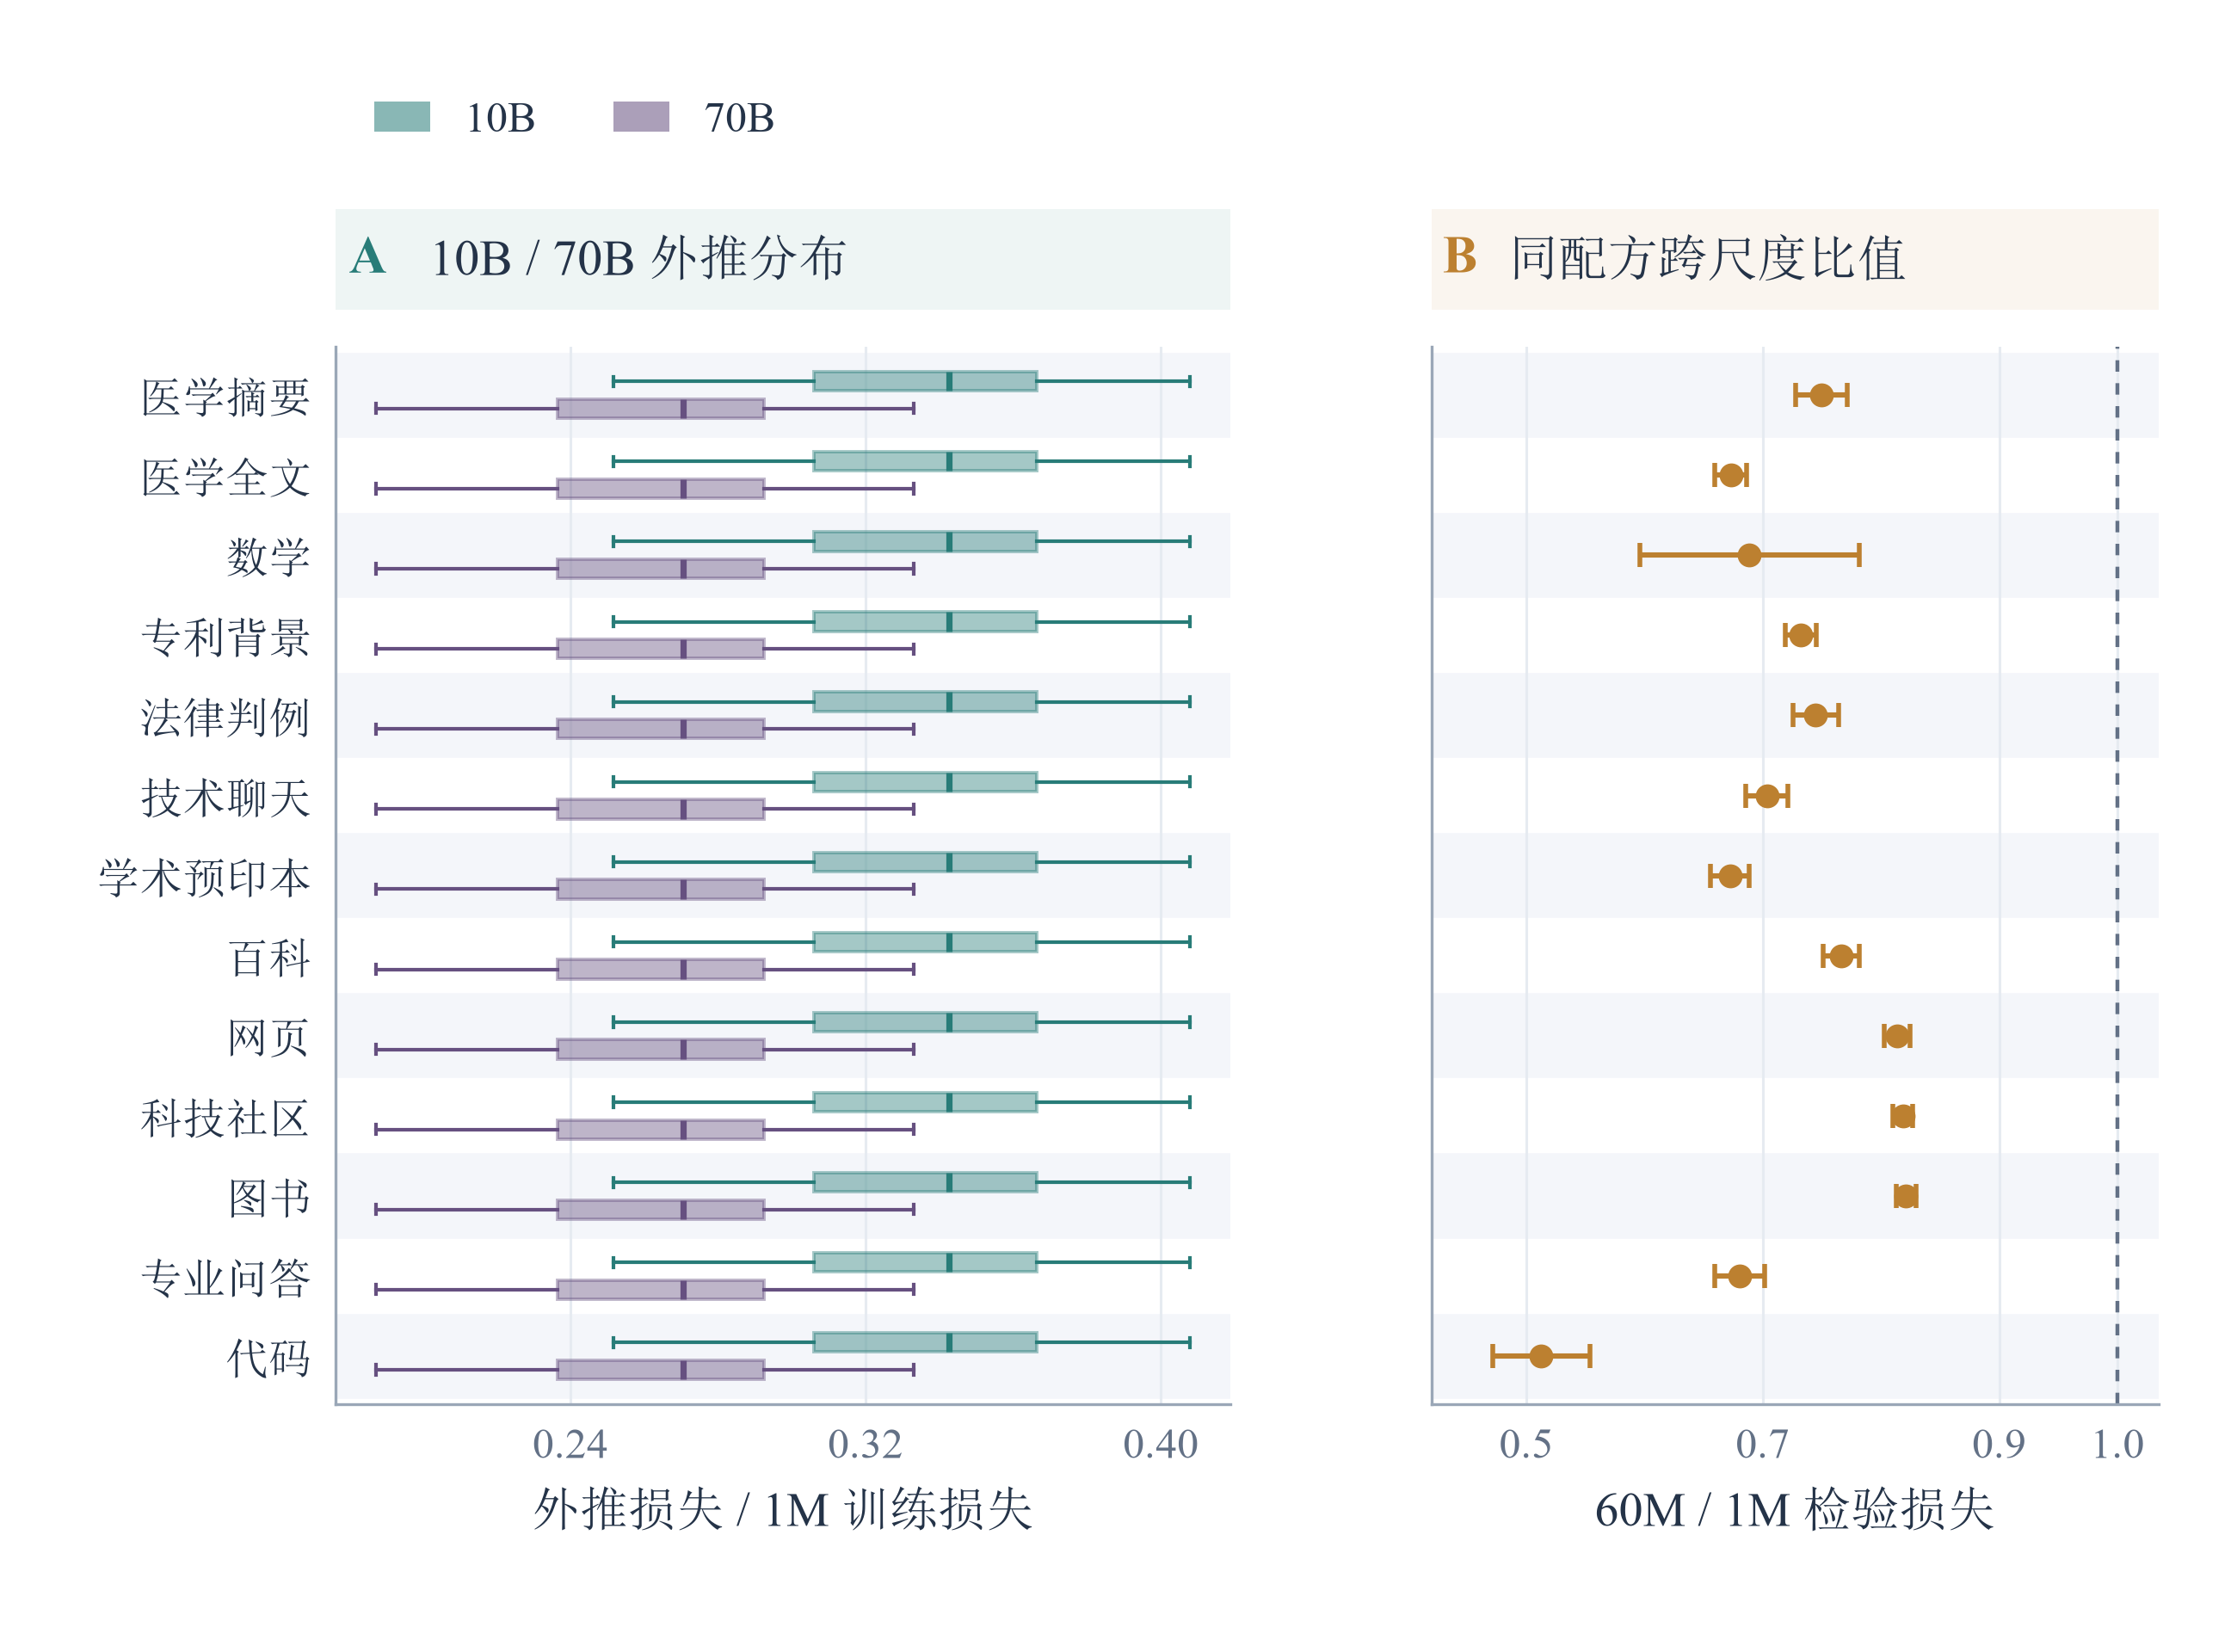
\includegraphics[width=0.92\textwidth]{../求解/问题一/图片/图7_外推与跨尺度.png}
  \caption{外推稳健性验证（左：10B 外推尺度因子；右：同配方 60M/1M 跨尺度损失比）}
  \label{fig:p1_extrap}
\end{figure}

本问得到各领域的质量分数、配比回归系数和有界推荐方案。质量对照说明评分依赖指标选择，跨规模检验说明损失还需进行尺度调整。后续资源配置将使用这些结果，并保留相应的适用条件。

\FloatBarrier
\endgroup

\Needspace{8\baselineskip}
\subsection{问题二：跨维度数据融合与广义标度律}
\begingroup
\setlength{\tabcolsep}{2pt}
\clubpenalty=10000
\widowpenalty=10000

\subsubsection{具体分析}

即使模型大小和训练数据量相同，换用不同语料后，验证损失也可能变化。因此，本问在规模关系之外加入质量和领域配比，进一步比较改善数据与增加参数能否取得相近效果。附件 A 记录配比实验，附件 B 记录规模与质量实验，两者没有同时观测全部变量，连接时需要说明评分是否可比、配比效果能否迁移。

我们的处理顺序见图\ref{fig:p2_framework}。先检查各数据集的用途和质量方向，再利用 Pythia 轨迹拟合规模关系，并把较大模型留出检验。随后对比四种质量表达，选择广义标度律，利用弹性和等损失公式解释质量投入的效果。最后接入问题一的配比系数，并用不同来源的检验结果说明模型适合在哪些条件下使用。

\begin{figure}[!htbp]
  \centering
  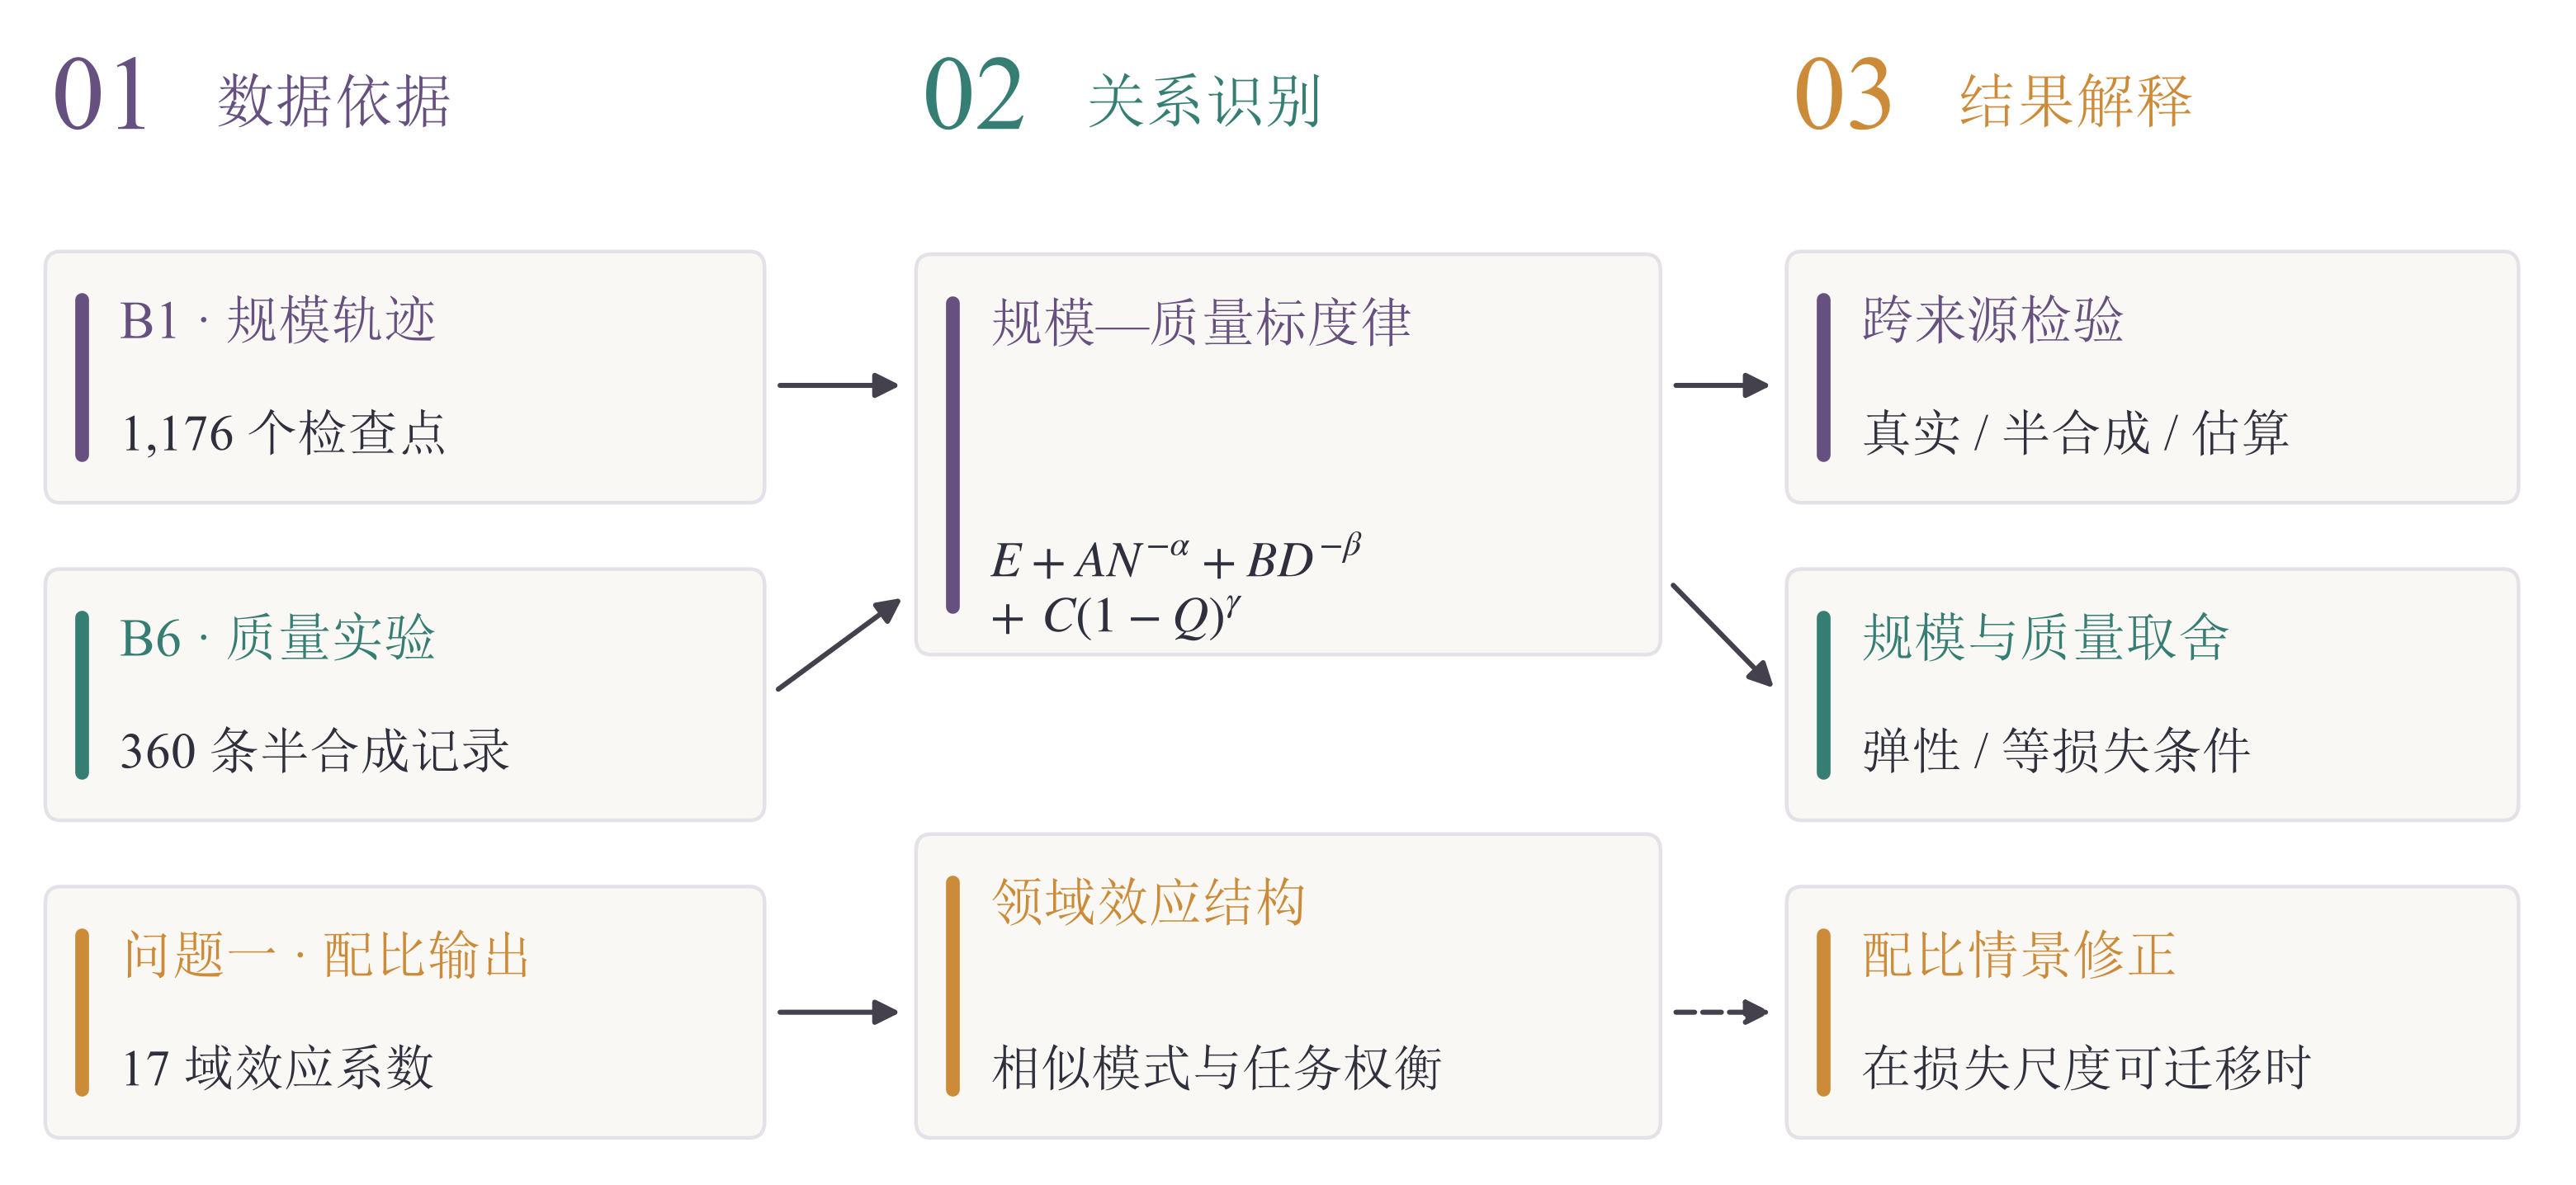
\includegraphics[width=0.98\textwidth]{../求解/问题二/图片/图0_问题二分析框架.png}
  \caption{规模、质量与领域效应的分析框架}
  \label{fig:p2_framework}
\end{figure}

\subsubsection{模型准备}

\textbf{1.数据组织与变量口径}\par\nopagebreak[4]
估计规模项采用 B1，其中包含 8 个 Pythia 模型，每个模型有 147 个检查点，共 1{,}176 条记录\cite{biderman2023pythia}。质量项采用 B6 半合成实验，B7 中与 B6 重复的记录不再用于扩展检验。其余附件分别承担对照作用：B2、B3 检查训练轨迹，B4、B5 检查跨族和文献数据，B8 检查质量评分是否同向；B9、B10 配对后用于比较大规模模型的估算损失。

我们用 $N$、$D$、$Q$ 分别表示参数量、训练数据量和质量，预测量为验证集交叉熵损失 $L$。本节的 $N$ 以十亿参数计，$D$ 以十亿 tokens 计；问题三计算算力时，两者均需乘以 $10^9$，恢复为绝对数量。拟合直接使用包含常数项 $E$ 的原函数，以保留不可约损失，避免取双对数时遗漏这一项。

\textbf{2.质量字段方向检验}\par\nopagebreak[4]
质量分数的含义需要先从数据中检查。固定每组实验的 $(N,D)$，计算组内 $Q_{\text{score}}$ 与损失的 Pearson 相关，再对各组系数取算术平均。平均相关为负，表示高评分通常对应低损失，符合本文的质量定义；若为正，则需要核对评分方向。表\ref{tab:p2_dir}中的均值只描述这一方向，不用于判断统计显著性。

\begin{table}[htbp]
  \centering
  \caption{质量评分方向与样本使用方式}
  \label{tab:p2_dir}
  \renewcommand{\arraystretch}{1.15}
  \setlength{\tabcolsep}{5pt}
  \begin{tabularx}{0.98\textwidth}{@{}
    >{\hsize=0.65\hsize\linewidth=\hsize\centering\arraybackslash}X
    >{\hsize=0.65\hsize\linewidth=\hsize\centering\arraybackslash}X
    >{\hsize=0.70\hsize\linewidth=\hsize\centering\arraybackslash}X
    >{\hsize=2.00\hsize\linewidth=\hsize\raggedright\arraybackslash}X@{}}
    \toprule
    数据分组 & \makecell{平均组内\\相关系数} & \makecell{记录数 /\\实验组数} & 评分解释与使用方式 \\
    \midrule
    B6 & $-0.925$ & 360 / 45 & 沿用原评分；$Q=1$ 为最优参考 \\
    B7 & $-0.918$ & 450 / 45 & 与 B6 同向，仅新增记录用于检验 \\
    B8 校准段 & $+0.995$ & 984 / 90 & 方向相反，翻转评分后作诊断 \\
    B8 外推段 & $+0.968$ & 720 / 60 & 方向相反，不纳入主拟合 \\
    \bottomrule
  \end{tabularx}
  \par\smallskip
  \begin{minipage}{0.98\textwidth}\normalsize
  注：实验组固定 $N,D$。B7 包含 B6 的全部 360 条记录，新增 90 条；均值只描述方向，不表示显著性。
  \end{minipage}
\end{table}

表中 B6 和 B7 分别得到 $-0.925$、$-0.918$，因此使用原评分 $Q=Q_{\text{score}}$。逐行比对发现，B7 已含 B6 的全部 360 条记录，只有另外 90 条可用于扩展检查，两套数据不能算作独立证据。B8 的两个子集方向相反，部分损失还低于本模型的下限。我们不把 B8 加入主拟合，只将评分改为 $1-Q_{\text{score}}$，检查翻转后是否仍存在偏差。

图\ref{fig:p2_direction}中，每个圆点对应一组固定 $(N,D)$ 的实验，菱形表示各组相关系数的平均值。B6/B7 的点大多在零点一侧，B8 则在另一侧，说明方向差异并非由少数组造成。B6 与 B7 的点群相近还与记录重叠有关，不能把这种接近当成新增的独立验证。

\begin{figure}[!htbp]
  \centering
  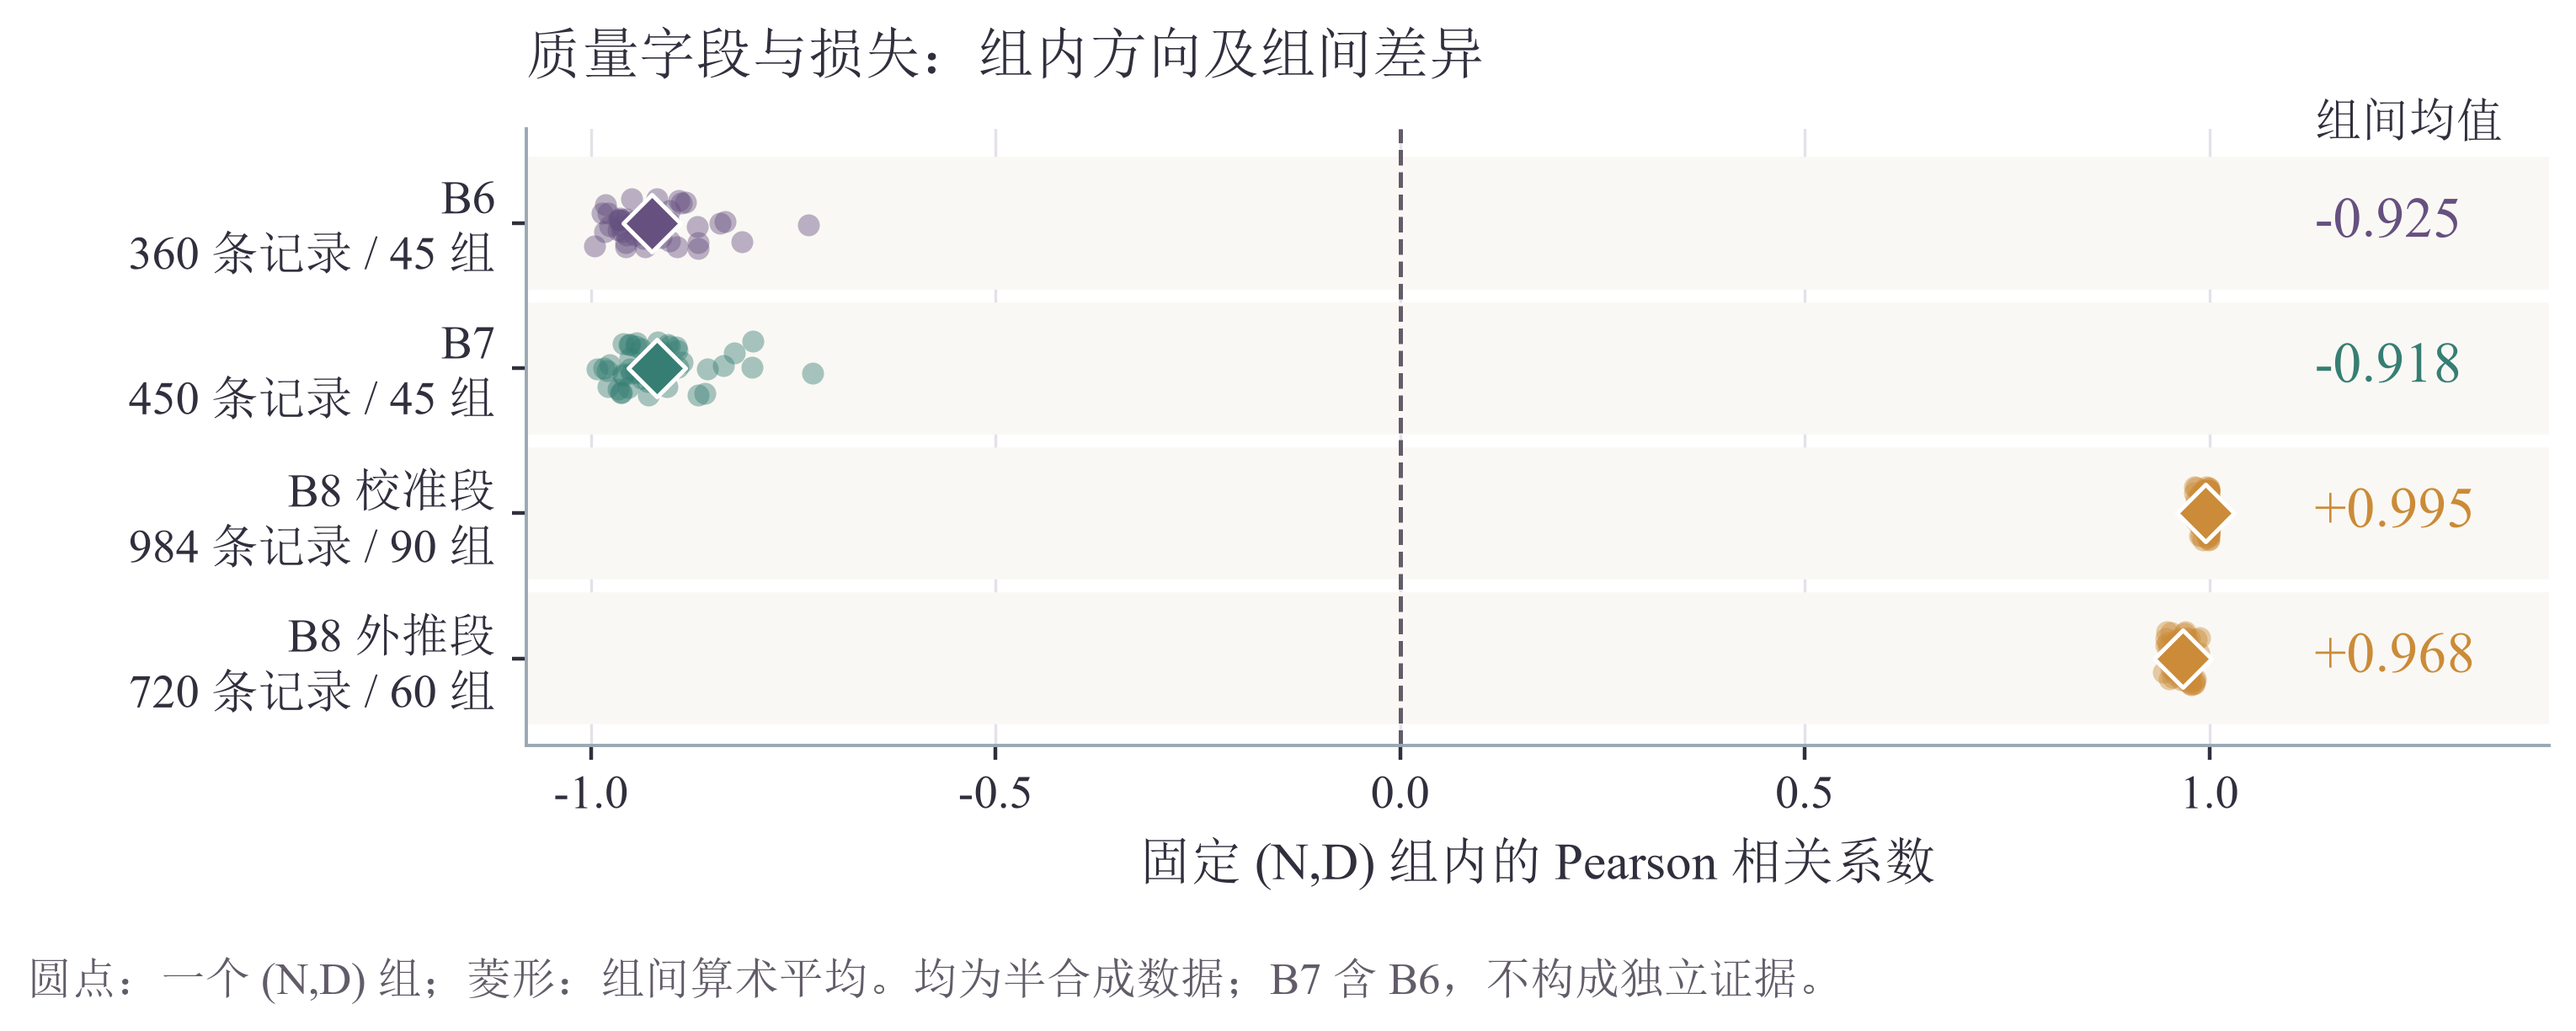
\includegraphics[width=0.98\textwidth]{../求解/问题二/图片/图7_质量方向对照.png}
  \caption{质量字段与损失的组内相关分布}
  \label{fig:p2_direction}
\end{figure}

\begin{samepage}
统一方向只解决了分数高低的含义，还不能保证不同评分可以直接互换。问题一的综合评分与附件 B 的 $Q_{\text{score}}$ 来自不同构造方法，相同分值未必对应相同质量。因此，本节的质量参数和数值解释均使用附件 B 的评分尺度。
\par
\end{samepage}

\subsubsection{模型建立}

\textbf{1.经典标度律}\par\nopagebreak[4]
先在参考质量下考察规模效应。采用 Chinchilla 标度律\cite{hoffmann2022chinchilla}，把验证损失 $L$ 写成参数量与数据量的函数：
\begin{equation}
    L(N,D) = E + \frac{A}{N^{\alpha}} + \frac{B}{D^{\beta}}
\end{equation}
式中，$E$ 是 $N,D\to\infty$ 时仍保留的损失。其余两项分别随参数量和数据量增加而下降，变化速度由 $\alpha$、$\beta$ 控制，幅度由 $A$、$B$ 控制。固定参考质量后，便可以分别比较增加参数和增加数据的收益。

\textbf{2.质量项的选择与损失修正}\par\nopagebreak[4]
加入质量有两种常见思路：让质量改变有效规模，或用单独一项表示质量不足的损失。本文在同一组联合样本上比较四种形式，依据 B6 的拟合、B7 新增点的预测相关和残差信息评分作选择，结果见表\ref{tab:p2_form}。各候选模型和经典模型均用带界约束的非线性最小二乘估计，保留常数与幂函数项，并采用 soft-$L_1$ 损失减轻大残差的影响。

\begin{table}[htbp]
  \centering
  \caption{不同质量作用形式的拟合与扩展检验指标}
  \label{tab:p2_form}
  \renewcommand{\arraystretch}{1.15}
  \begin{tabularx}{0.98\textwidth}{@{}>{\raggedright\arraybackslash}X*{4}{>{\centering\arraybackslash}p{0.17\textwidth}}@{}}
    \toprule
    比较指标 & \makecell{加性质量缺口\\$C(1-Q)^\gamma$} & \makecell{质量同时乘\\$N$ 与 $D$} & \makecell{加性质量亏损\\$CQ^{-\gamma}$} & \makecell{质量作为\\有效数据乘子} \\
    \midrule
    联合样本 $R^2$ & \textbf{0.9896} & 0.9882 & 0.9848 & 0.9745 \\
    B6 样本 $R^2$ & \textbf{0.9556} & 0.9495 & 0.9349 & 0.8905 \\
    B7 新增点 $r$ & 0.991 & \textbf{0.991} & 0.991 & 0.983 \\
    待估参数个数 & 7 & 7 & 7 & 6 \\
    残差信息评分 $I_{\mathrm{RSS}}$ & $\mathbf{-10236}$ & $-10042$ & $-9660$ & $-8866$ \\
    \bottomrule
  \end{tabularx}
  \par\smallskip
  \begin{minipage}{0.98\textwidth}\normalsize
  注：相关系数保留三位小数；加粗的最优指标按未舍入值确定。$I_{\mathrm{RSS}}$ 越小越优，仅用于同样本比较。
  \end{minipage}
\end{table}

\begin{samepage}
四种形式在 B7 新增点上的相关系数都不低于 $0.983$，这一指标不足以单独决定选择。表\ref{tab:p2_form}中，加性质量缺口形式在联合样本和 B6 上的 $R^2$ 均最高，因此采用该形式。后续同时报告 RMSE 和 MAPE，检查较高相关是否伴随较小的实际预测误差。
\par
\end{samepage}

\begin{samepage}
残差信息评分采用 $I_{\mathrm{RSS}}=n\ln(\mathrm{RSS}/n)+2k$，其中 $n$ 为样本数，$k$ 为参数数。参数通过 soft-$L_1$ 而非高斯极大似然估计，所以该值只用于相同样本下的辅助比较，不按严格的 AIC 解释。另外，B7 新增记录既参与形式选择，也参与扩展检查，其结果属于开发阶段验证，不能作为完全独立的最终测试。
\par
\end{samepage}

将选定的质量缺口项加入规模基线后，损失关系写为：
\begin{equation}
    L(N,D,Q) = E + \frac{A}{N^{\alpha}} + \frac{B}{D^{\beta}} + C\,(1-Q)^{\gamma},
    \qquad C>0,\ \gamma>0
\end{equation}
\begin{samepage}
将 $Q=1$ 设为质量参考点，使质量项在此处归零，广义模型便恢复经典标度律的形式。联合拟合会重新估计参数，不要求与经典拟合值相同。Pythia 没有质量实测值，赋予 $Q=1$ 也仅表示这一参考约定。固定 $Q$，令参数和数据量同时增大，可得
\par\nopagebreak[4]
\begin{equation}
    \lim_{N,D\to\infty} L(N,D,Q) = E + C\,(1-Q)^{\gamma} \;\ge\; E
\end{equation}
\end{samepage}
由此可见，只要质量固定在 $Q<1$，扩大模型和增加数据都只能降低各自的规模项，质量缺口仍然存在。因此，在本加性模型中，规模投入不能完全消除质量不足的影响。该判断是函数结构的结果，应用到实际训练仍需考虑拟合范围。

\textbf{3.边际效用与弹性}\par\nopagebreak[4]
为刻画各因素微小变化对损失的影响，对广义模型求偏导，并在参考点 $(N_0,D_0,Q_0)$ 处评价：
\begin{equation}
    \frac{\partial L}{\partial N} = -\alpha A N^{-\alpha-1},\quad
    \frac{\partial L}{\partial D} = -\beta B D^{-\beta-1},\quad
    \frac{\partial L}{\partial Q} = -\gamma C (1-Q)^{\gamma-1}
\end{equation}
各偏导的单位不同。令参考点的预测损失为 $L_0$，按变量与损失的比例变化定义弹性：
\begin{equation}
    \varepsilon_N = \frac{\partial L}{\partial N}\frac{N_0}{L_0},\qquad
    \varepsilon_D = \frac{\partial L}{\partial D}\frac{D_0}{L_0},\qquad
    \varepsilon_Q = \frac{\partial L}{\partial Q}\frac{Q_0}{L_0}
\end{equation}

\textbf{4.质量提升与参数扩张的等效条件}\par\nopagebreak[4]
为了比较两种投入，固定 $D$ 与领域配比，并选择相同的初始配置。若少量提高质量和少量增加参数带来的损失降幅相等，就可用正向增量比 $R_{NQ}$ 表示其等效关系：
\begin{equation}
    \begin{aligned}
      \left|\frac{\partial L}{\partial Q}\right|\mathrm dQ
      &=\left|\frac{\partial L}{\partial N}\right|\mathrm dN_{\mathrm{eq}},\\
      R_{NQ}=\frac{\mathrm dN_{\mathrm{eq}}}{\mathrm dQ}
      &=\frac{\gamma C(1-Q)^{\gamma-1}}{\alpha A N^{-\alpha-1}}
       =\frac{\gamma C}{\alpha A}(1-Q)^{\gamma-1}N^{\alpha+1}.
    \end{aligned}
\end{equation}
$R_{NQ}$ 比较的是两种改善方案各自需要的增量。若要求损失保持不变，则应写为 $\mathrm dN/\mathrm dQ=-R_{NQ}$，即提高质量后可以减少参数。固定 $Q$ 时，该比值随 $N^{\alpha+1}$ 增长，因为大模型继续扩容的边际收益较小。这里的“等效”只针对损失，实际算力是否相等还要比较语料处理和训练成本。

当质量变化 $\Delta Q$ 不够小时，需要直接计算完整损失差。记质量改善带来的降幅为 $\delta_Q$，令参数扩张取得相同降幅，解得
\begin{equation}
  \begin{aligned}
    \delta_Q &= C\bigl[(1-Q)^\gamma-(1-Q-\Delta Q)^\gamma\bigr],\\
    \Delta N_{\mathrm{eq}}
      &= N\left[\left(1-\frac{\delta_Q N^\alpha}{A}\right)^{-1/\alpha}-1\right].
  \end{aligned}
  \label{eq:p2_finite}
\end{equation}
首先要求 $0<\Delta Q\leq1-Q$，以免质量超过上界。其次，只有 $\delta_Q<AN^{-\alpha}$ 时，才能找到有限的等效参数增量；两者相等时需要无限参数，前者更大时则没有仅靠扩容的等效解。原因是当前参数项 $AN^{-\alpha}$ 已是扩容所能消除的全部损失。当 $\Delta Q\to0$，上式回到局部近似 $\Delta N_{\mathrm{eq}}\approx R_{NQ}\Delta Q$；计算结果若超过拟合规模，仍需按外推看待。


\textbf{5.领域效应的相似性}\par\nopagebreak[4]
同一训练领域在不同验证任务上的作用也可能不同。问题一给出了领域 $i$、$j$ 在 13 个任务上的系数向量 $\bm a_i,\bm a_j$。先减去平均向量，再用余弦相似度比较它们的相对作用：
\begin{equation}
    s_{ij} = \frac{\langle \bm a_i-\bar{\bm a},\ \bm a_j-\bar{\bm a}\rangle}{\|\bm a_i-\bar{\bm a}\|\,\|\bm a_j-\bar{\bm a}\|}
\end{equation}
$\bar{\bm a}$ 为 17 个训练领域系数向量的均值。$s_{ij}\to1$ 表示两域的相对作用方向接近，$s_{ij}\to-1$ 表示方向相反，可能涉及不同任务之间的取舍。余弦值没有保留作用大小，原回归也没有领域交互项。因此，仅凭相似度还不能确定两域可以等量替换，或联合使用后会获得额外收益。

\subsubsection{模型求解}

\noindent\textbf{辅助分析说明：} 本问数据整理、绘图与数值核对使用 Codex 辅助，模型为 GPT-5.4（OpenAI，2026-03-05）及 GPT-6 系列（OpenAI，2026-09-03 系列首次发布）\cite{ai_codex54,ai_codex6}。

\begin{samepage}
\textbf{1.经典标度律拟合与留出验证}\par\nopagebreak[4]
首先用 B1 的 1{,}176 条记录估计经典模型。图\ref{fig:p2_classic}左侧展示损失与两类规模的关系，右侧比较不同规模模型的残差，拟合得到
\begin{equation}
    L(N,D) = 1.6898 + \frac{0.3540}{N^{0.3400}} + \frac{1.2403}{D^{0.2799}}
\end{equation}
全部记录的拟合结果为 $R^2 = 0.9999998$、RMSE $=1.5\times10^{-4}$、MAPE $=0.004\%$。随后只用最小的 4 个模型重新估计，并预测留出的 4 个较大模型，得到 $R^2=0.9999997$、MAPE $=0.005\%$。误差仍较小，说明这一规模关系在所考察的 Pythia 模型族内保持稳定。
\par
\end{samepage}

\begin{figure}[!htbp]
  \centering
  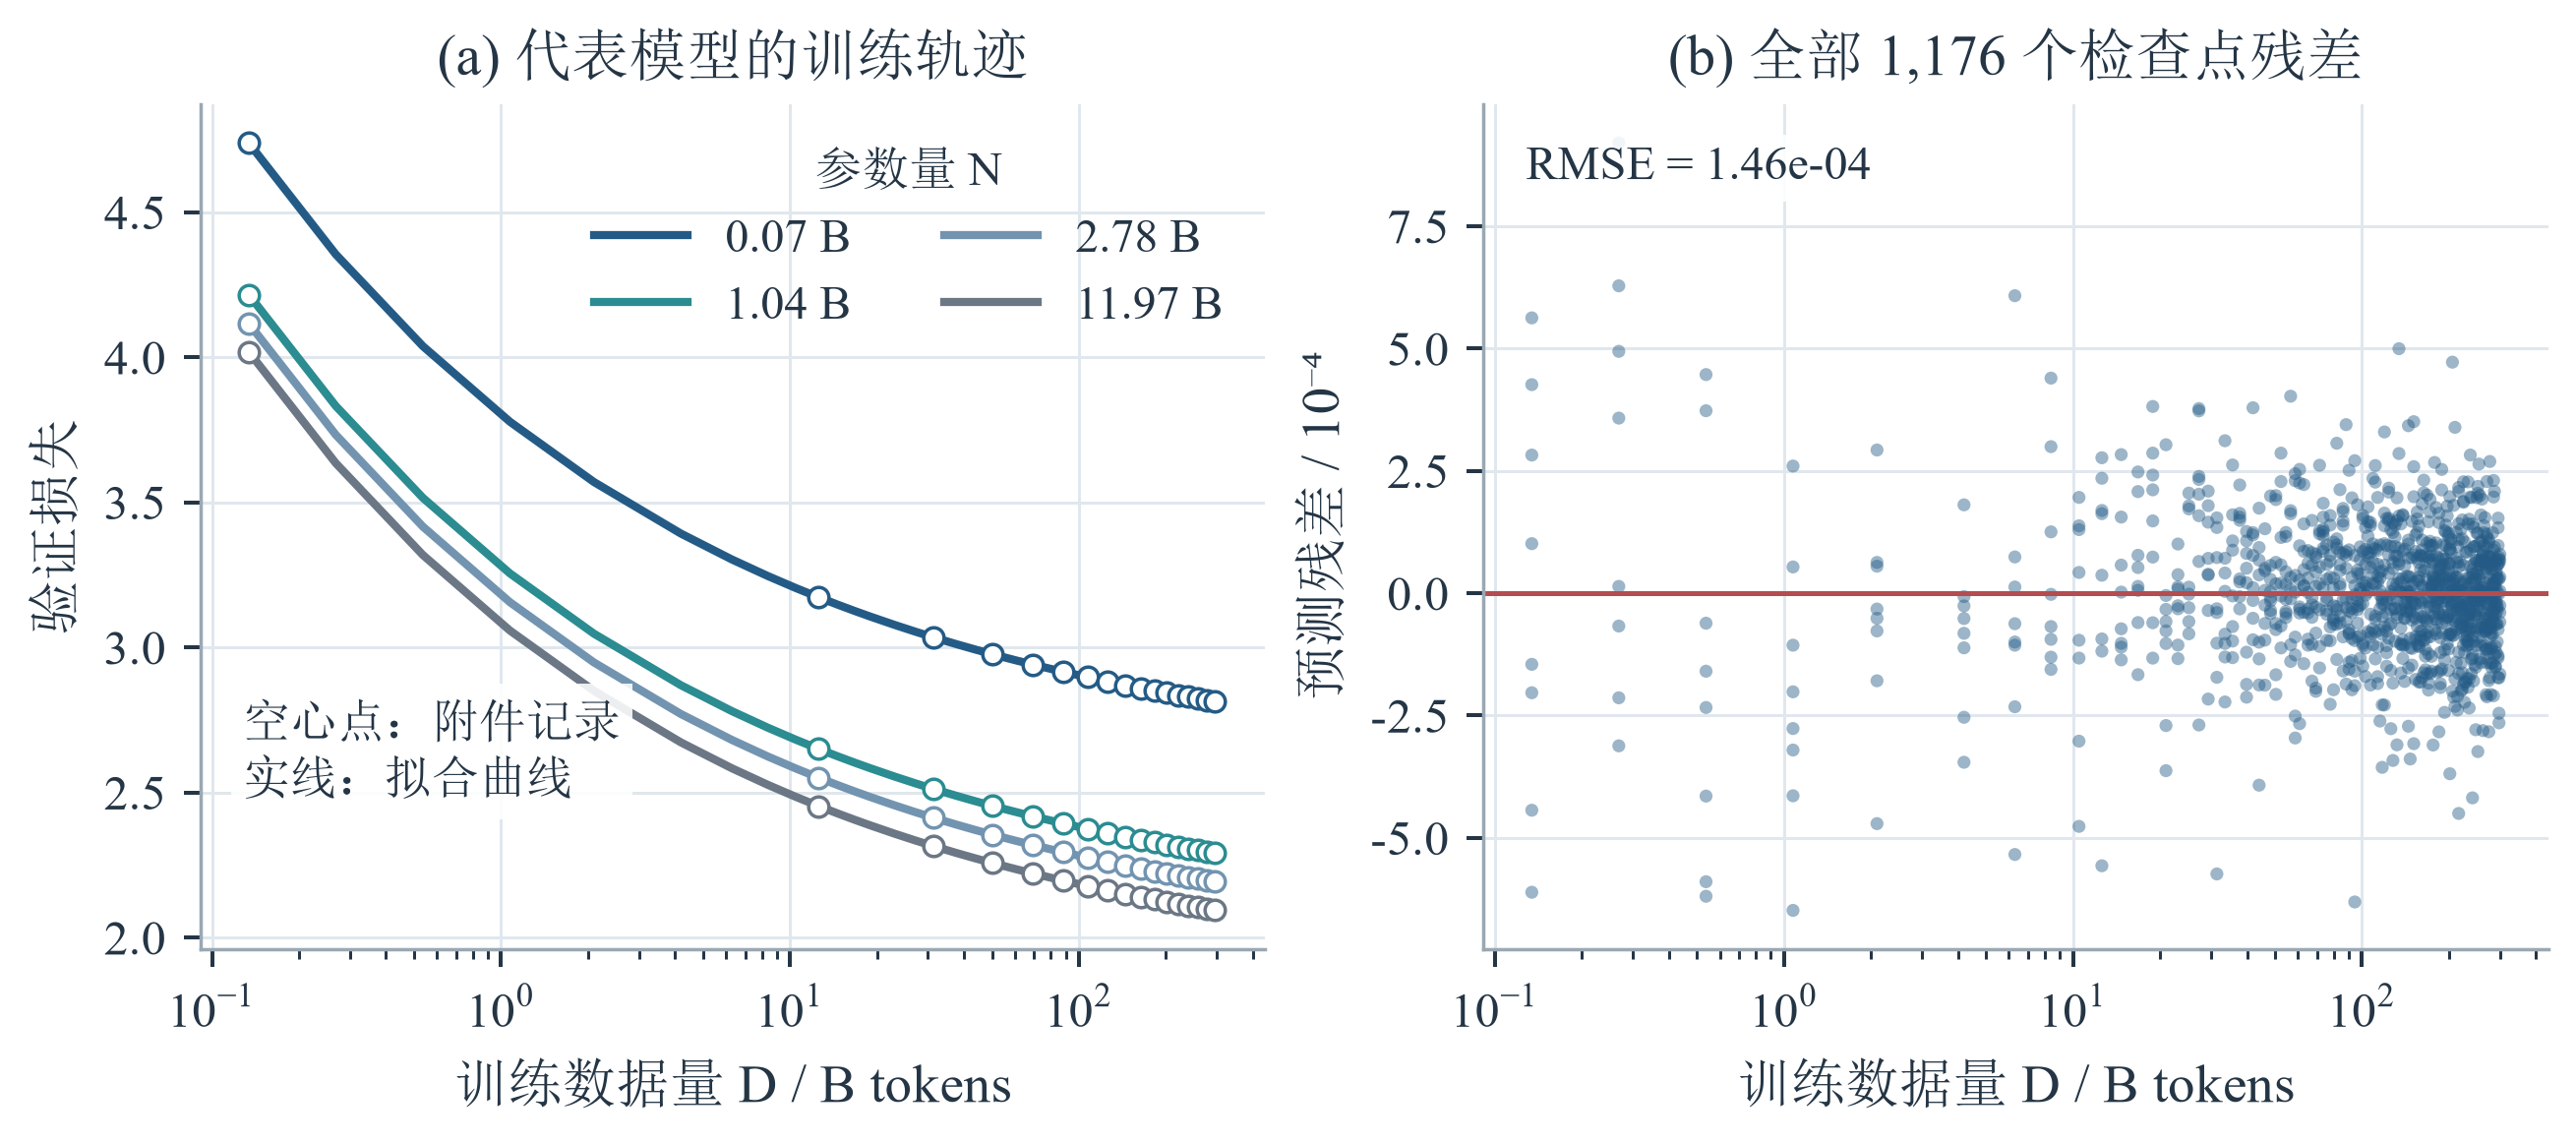
\includegraphics[width=0.98\textwidth]{../求解/问题二/图片/图1_经典标度律拟合.png}
  \caption{Pythia 规模--损失地图与分模型残差分布}
  \label{fig:p2_classic}
\end{figure}

残差标准差只有 $1.5\times10^{-4}$，远小于损失本身的标准差 $0.342$，所选函数与 B1 记录非常接近。但这还不能说明换用数据来源后仍有同等精度，故继续使用 B4、B5 外部数据和 B2 半合成轨迹检查。

\begin{samepage}
B3 可用于检查数据项的指数是否一致。分别固定 8 条插值轨迹的 $N$，先从损失中扣除 $E+AN^{-\alpha}$，再对 $L-(E+AN^{-\alpha})$ 与 $D$ 作双对数回归。所得指数为 $-0.2806\sim-0.2803$，与 $-\beta=-0.2799$ 接近。由于这些轨迹由 Pythia 检查点插值得到，结果说明内部关系一致，并不增加独立观测。
\par
\end{samepage}

\textbf{2.广义标度律参数估计}\par\nopagebreak[4]
再将 Pythia 的规模记录与 B6 质量实验合并，估计表\ref{tab:p2_form}选出的广义形式。对没有质量实测值的 Pythia 仍按约定取 $Q=1$，各项系数和指数列于表\ref{tab:p2_params}。

\begin{table}[H]
  \centering
  \caption{广义模型各损失项的参数配置}
  \label{tab:p2_params}
  \renewcommand{\arraystretch}{1.15}
  \setlength{\tabcolsep}{5pt}
  \begin{tabularx}{0.94\textwidth}{@{}*{5}{>{\centering\arraybackslash}X}@{}}
    \toprule
    损失组成 & 系数符号 & 系数估计 & 指数符号 & 指数估计 \\
    \midrule
    不可约损失 & $E$ & 1.6558 & -- & -- \\
    参数规模项 & $A$ & 0.3808 & $\alpha$ & 0.3266 \\
    训练数据项 & $B$ & 1.2515 & $\beta$ & 0.2767 \\
    质量缺口项 & $C$ & 0.3544 & $\gamma$ & 0.9779 \\
    \bottomrule
  \end{tabularx}
  \par\smallskip
  \begin{minipage}{0.94\textwidth}\normalsize
  注：联合拟合 $R^2=0.9896$；不可约损失为常数项，不含衰减指数。
  \end{minipage}
\end{table}

\begin{samepage}
联合估计得到 $R^2=0.9896$、RMSE $=0.036$ 和 MAPE $=0.66\%$。表\ref{tab:p2_params}中的 $\gamma=0.9779\approx1$，表示质量缺口扩大时，渐近损失近似按线性关系增加。这里增加了质量实验，样本已不同于经典拟合，所以不能用两个 $R^2$ 的差值衡量加入质量项的收益。
\par
\end{samepage}

\begin{samepage}
图\ref{fig:p2_quality}说明质量对损失的影响。左图固定 $D=300$B tokens，用底色和等值线表示不同规模、质量组合的预测损失，空心点为 B6 实验位置；右图以 $E$ 为起点，展示质量不足使损失下限增加多少。
\par
\end{samepage}

根据 $E+C(1-Q)^{\gamma}$，$Q=1$ 时损失下限为 $1.656$。质量分别降到 $Q=0.6$、$Q=0.3$ 后，下限提高至 $1.801$、$1.906$。

\begin{figure}[!htbp]
  \centering
  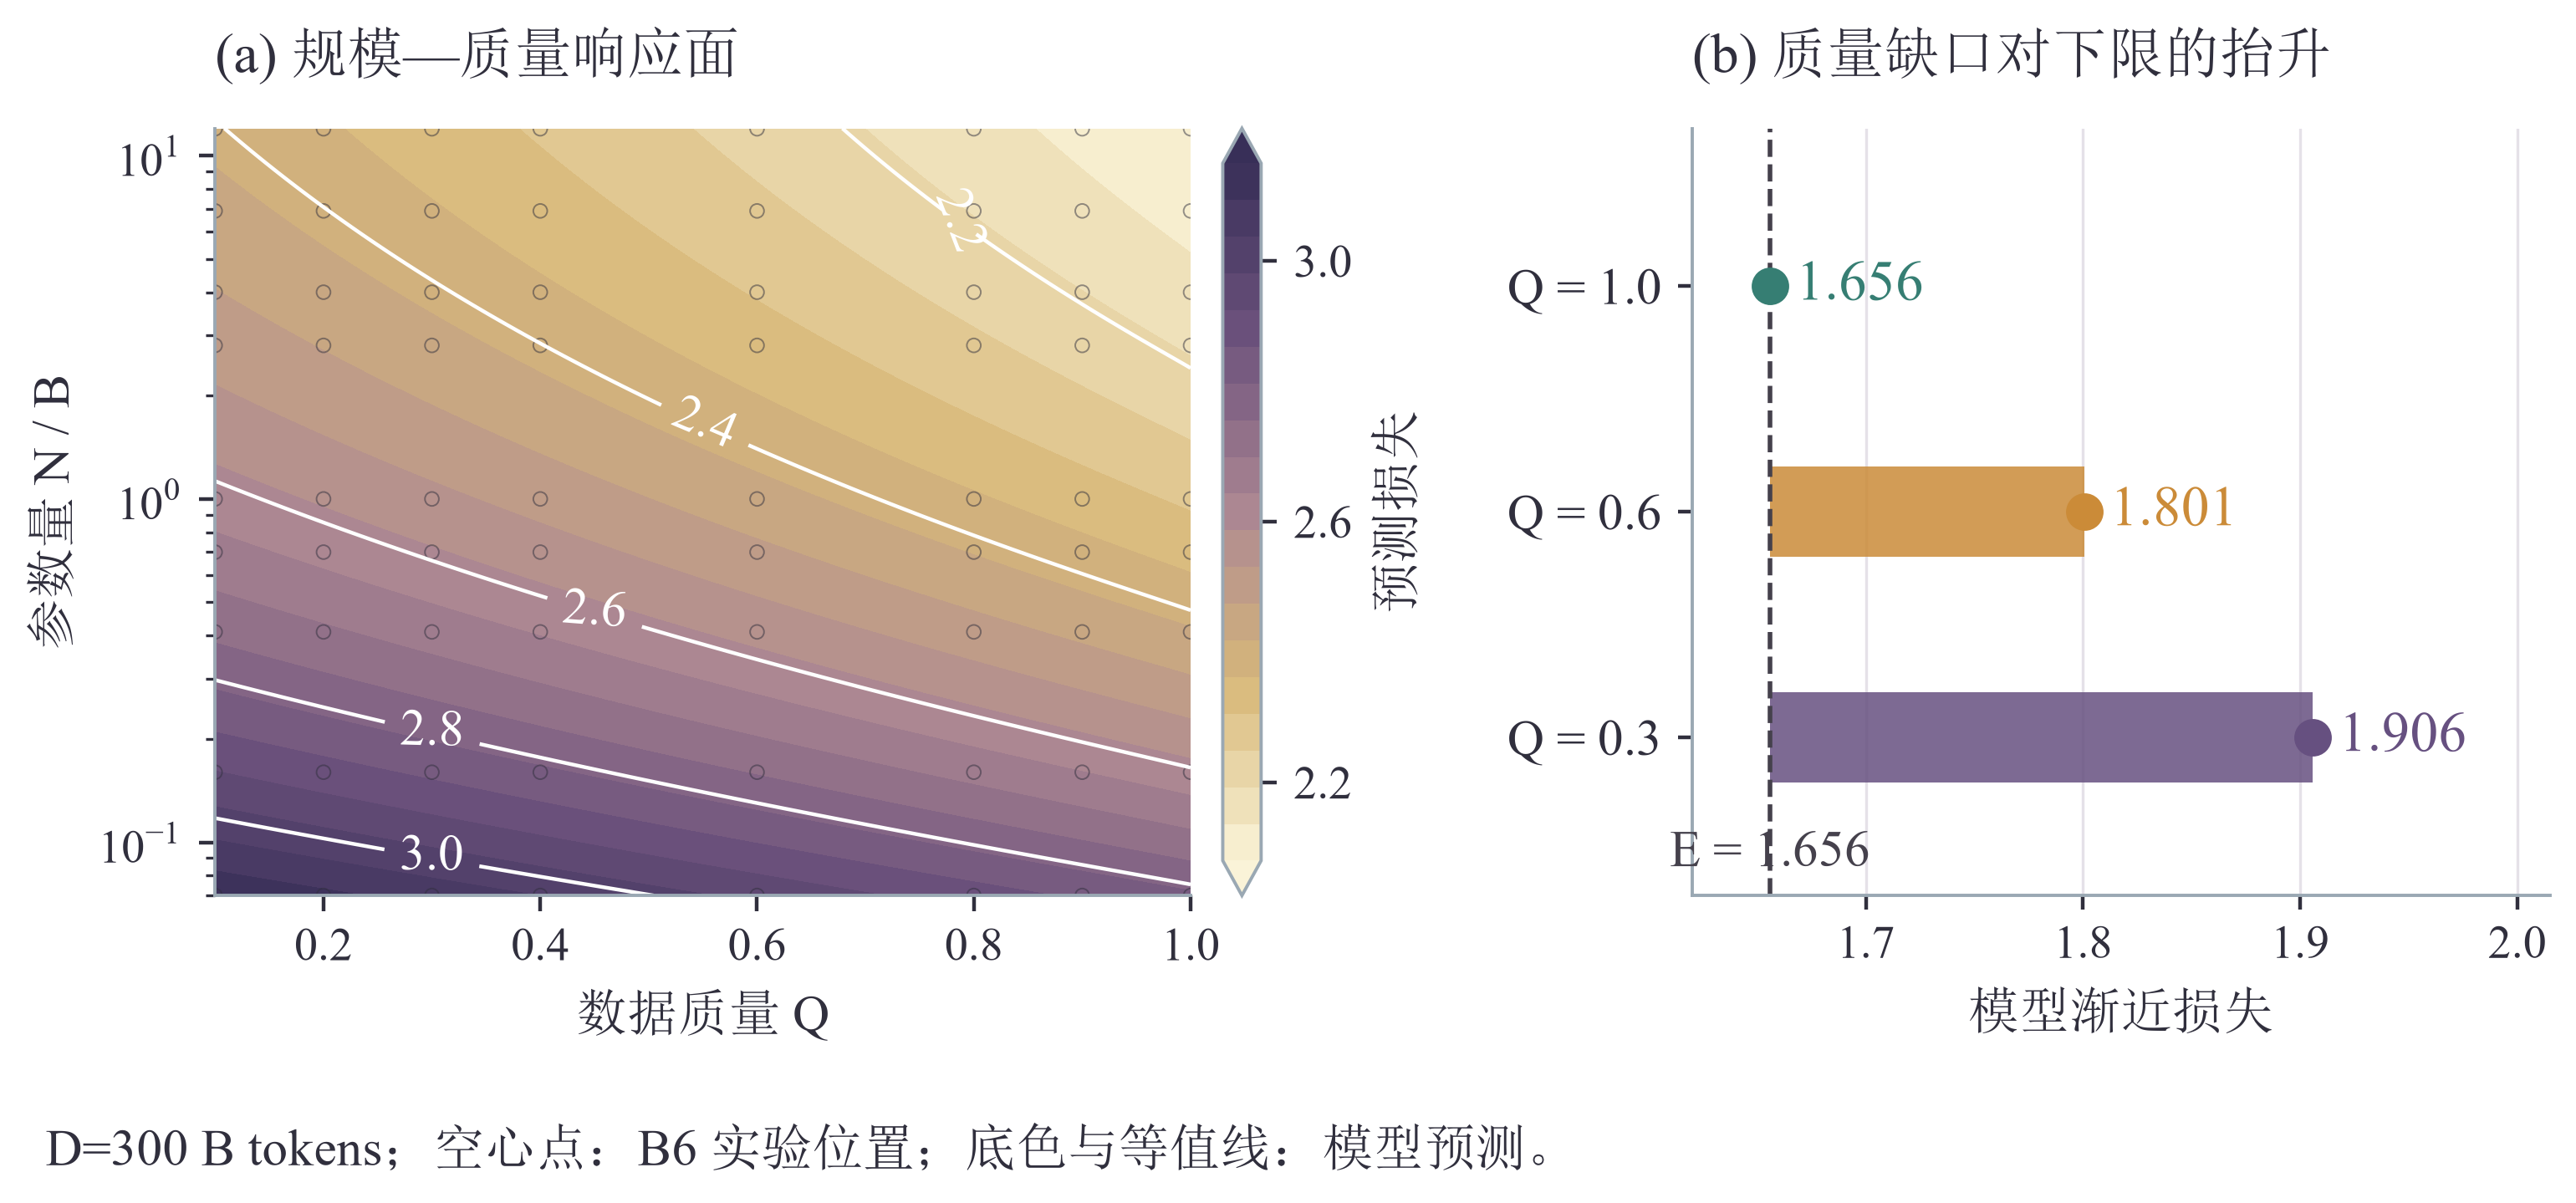
\includegraphics[width=0.98\textwidth]{../求解/问题二/图片/图3_质量边际影响.png}
  \caption{规模--质量响应面与渐近损失分解}
  \label{fig:p2_quality}
\end{figure}

\textbf{3.分层检验与适用范围}\par\nopagebreak[4]
配置计算依赖模型预测，因此还需比较不同来源上的误差。表\ref{tab:p2_val}汇总 6 组检验的 MAPE、RMSE 和相关系数，图\ref{fig:p2_general}展示 $100(\hat L-L)/L$ 的分布：负值为低估，正值为高估。为同时看清小误差和大偏差，图中横轴在 $\pm10\%$ 内采用线性刻度，外侧改用对称对数刻度。

\begin{table}[htbp]
  \centering
  \caption{按数据性质区分的预测误差与相关性}
  \label{tab:p2_val}
  \renewcommand{\arraystretch}{1.15}
  \setlength{\tabcolsep}{5pt}
  \begin{tabularx}{0.98\textwidth}{@{}
    >{\hsize=0.75\hsize\linewidth=\hsize\centering\arraybackslash}X
    >{\hsize=2.25\hsize\linewidth=\hsize\raggedright\arraybackslash}X
    >{\hsize=0.75\hsize\linewidth=\hsize\centering\arraybackslash}X
    >{\hsize=0.80\hsize\linewidth=\hsize\centering\arraybackslash}X
    >{\hsize=0.75\hsize\linewidth=\hsize\centering\arraybackslash}X
    >{\hsize=0.70\hsize\linewidth=\hsize\centering\arraybackslash}X@{}}
    \toprule
    数据性质 & 对照样本 & 记录数 & MAPE/\% & RMSE & $r$ \\
    \midrule
    \multirow{2}{*}{真实} & B4 跨模型族收敛点 & 57 & 8.8 & 0.293 & 0.975 \\
      & B5 文献标度记录 & 44 & 8.0 & 0.193 & 0.910 \\
    \addlinespace[3pt]
    \multirow{3}{*}{半合成} & B7 新增质量实验 & 90 & 1.6 & 0.056 & 0.991 \\
      & B2 Cerebras 轨迹 & 1{,}029 & 33.7 & 1.245 & 0.666 \\
      & B8 校准段（方向变换） & 984 & 133.4 & 1.294 & 0.638 \\
    \addlinespace[3pt]
    估算 & B10 大规模估算损失 & 128 & 1.0 & 0.020 & 1.000 \\
    \bottomrule
  \end{tabularx}
  \par\smallskip
  \begin{minipage}{0.98\textwidth}\normalsize
  注：B8 使用 $1-Q_{\text{score}}$；B10 统一取 $Q=1$。B7 属于开发阶段验证，B10 不构成独立实验验证。
  \end{minipage}
\end{table}

\begin{figure}[!htbp]
  \centering
  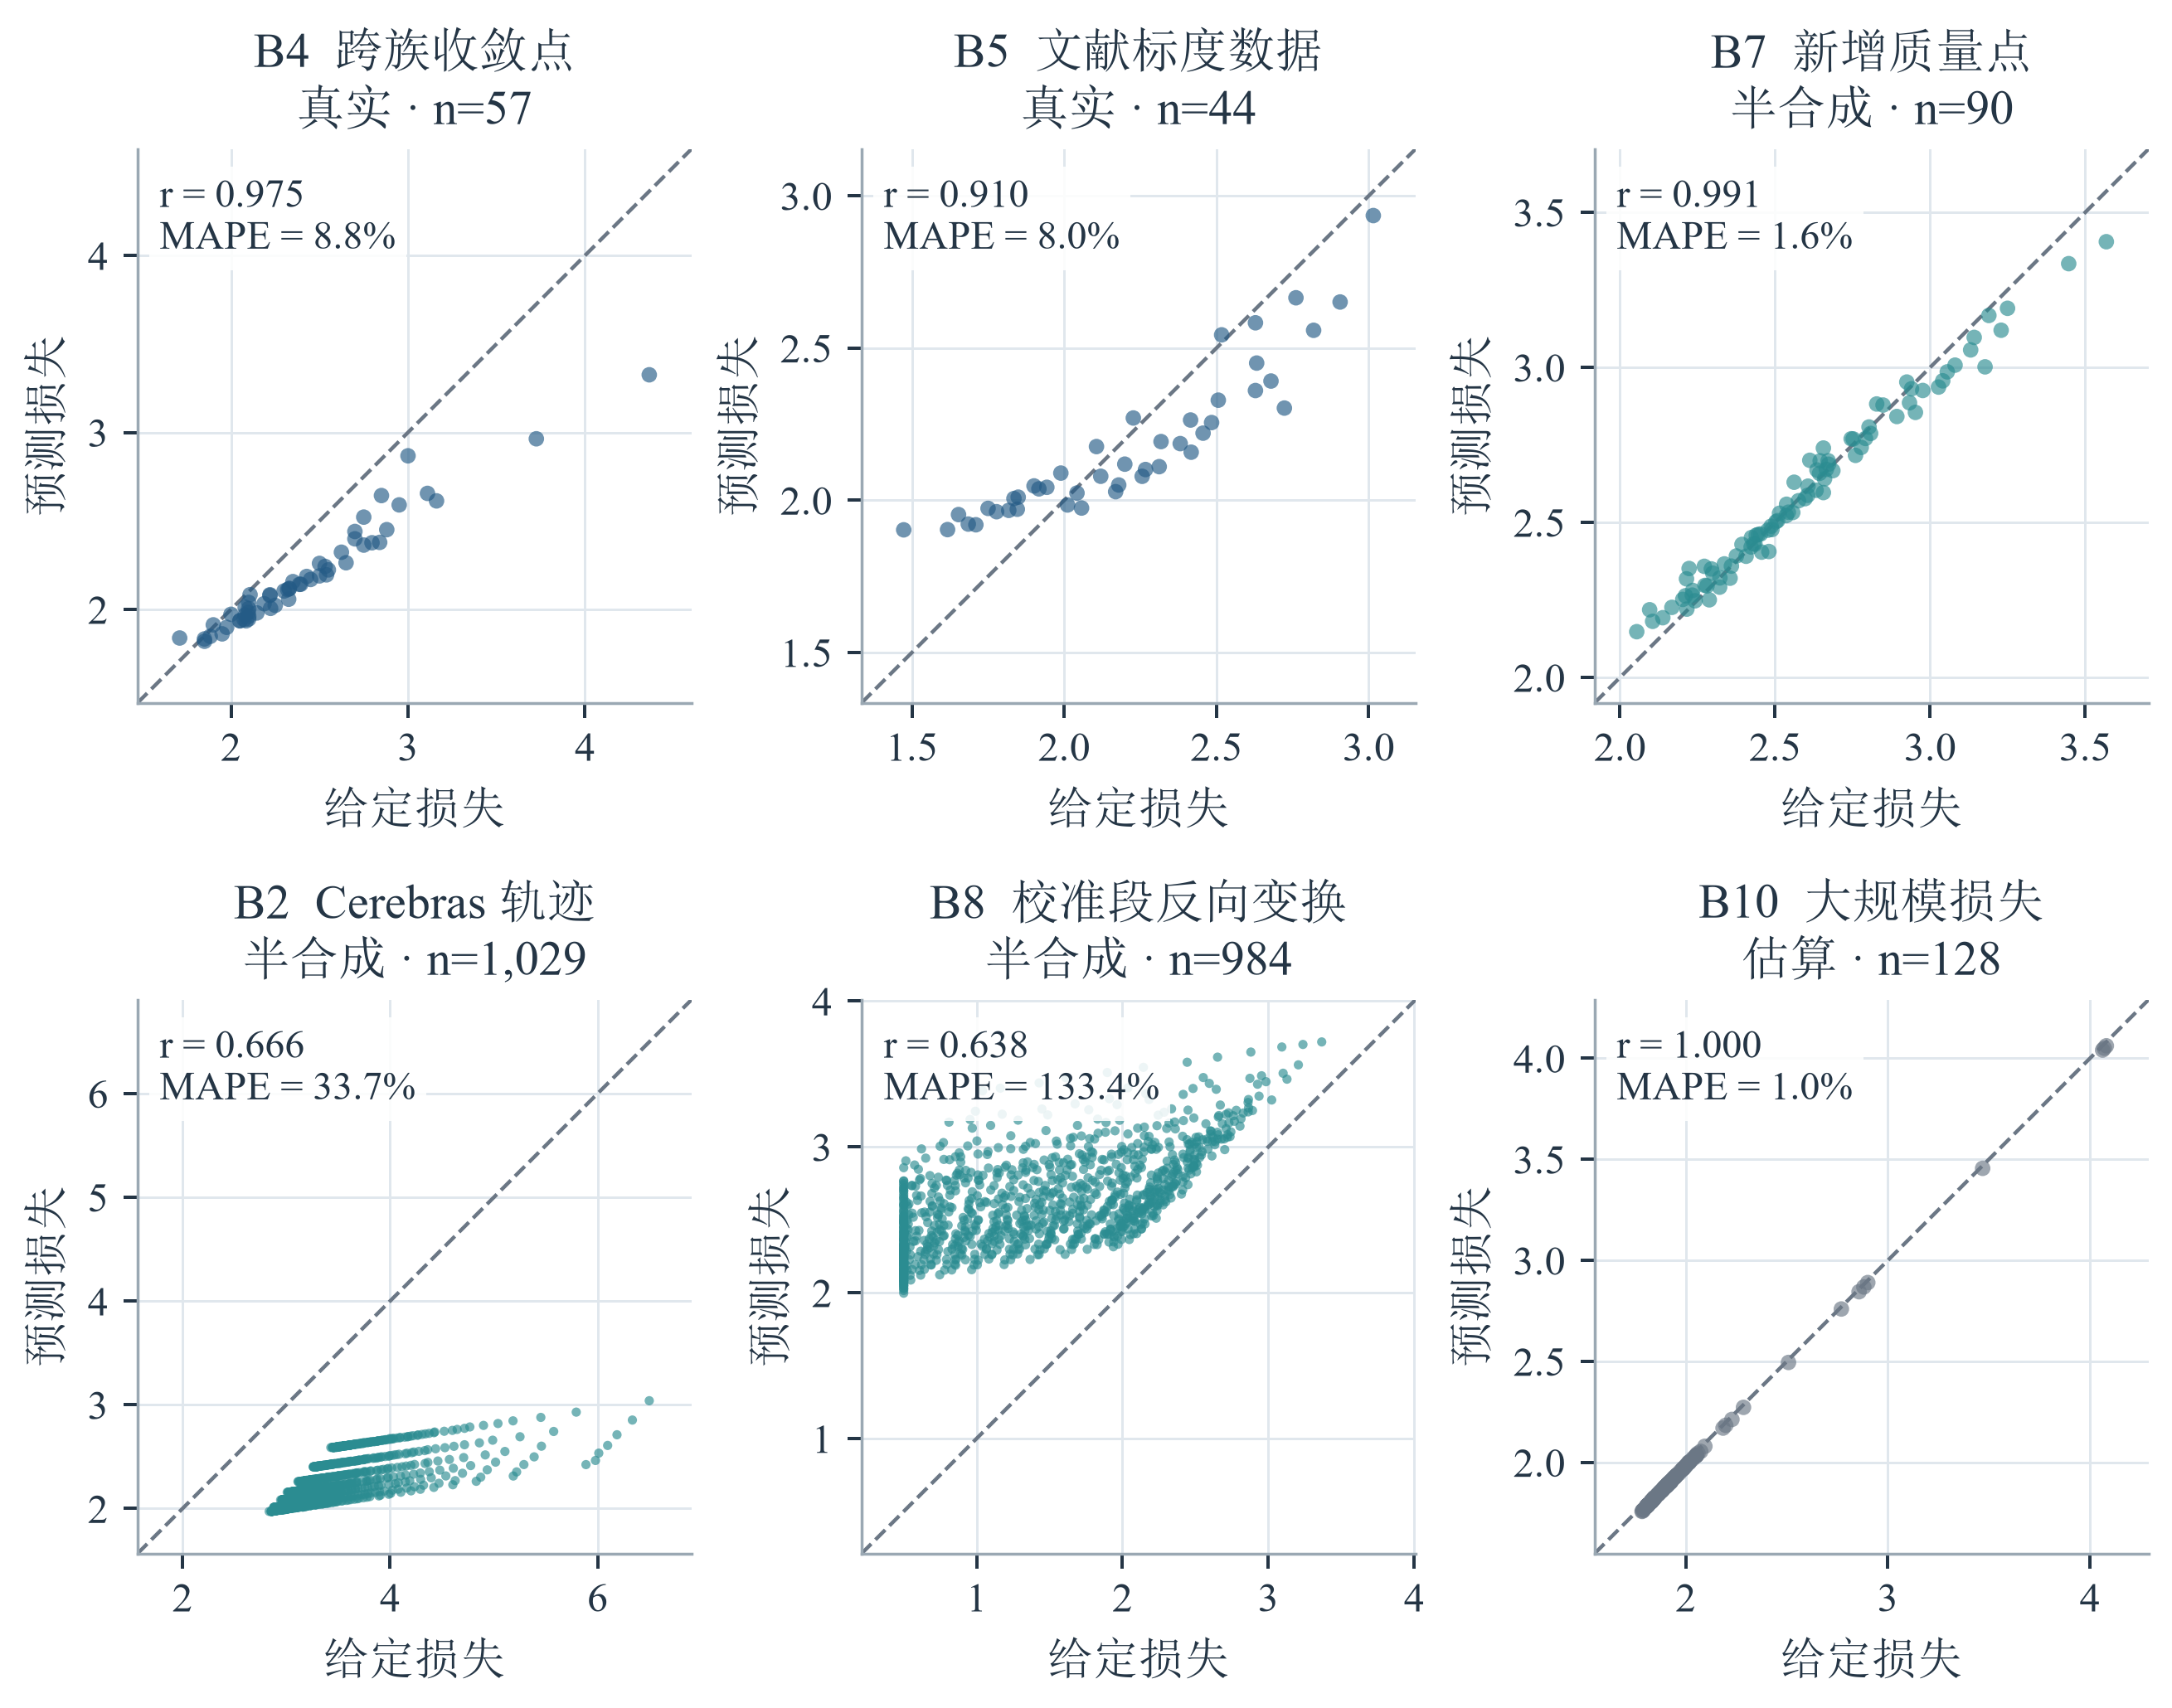
\includegraphics[width=0.98\textwidth]{../求解/问题二/图片/图2_广义标度律验证.png}
  \caption{不同数据来源的有符号相对误差分布}
  \label{fig:p2_general}
\end{figure}

\begin{samepage}
表\ref{tab:p2_val}中，B4 与 B5 的相关系数分别为 $0.975$、$0.910$，MAPE 分别为 $8.8\%$、$8.0\%$。两组结果表明，模型能够跟随部分跨族规模变化，但具体损失值仍有偏差，使用时不能只看相关性高低。
\par
\end{samepage}

\begin{samepage}
B7 的 90 个新增点得到 MAPE $1.6\%$，表明质量关系在同一半合成设定下可作一定扩展。B10 的损失来自估算，对照时统一取 $Q=1$，因而只检查估算关系是否接近，既不检验质量项，也不能作为独立实验。
\par
\end{samepage}

\begin{samepage}
B2 的 MAPE 为 $33.7\%$，B8 校准段在翻转评分后仍达 $133.4\%$。B8 还包含低于本模型渐近下限的损失。可见，改变质量方向并不足以统一这些来源，损失尺度或数据生成方式的差别仍会限制模型使用。
\par
\end{samepage}

\begin{samepage}
数值结论应结合估计所覆盖的范围使用。B1 的 $N$ 约为 $0.07$--$12$B，$D$ 为 $0.134$--$299.893$B tokens；B6 对应 $0.07$--$11.97$B 和 $10$--$600$B tokens。质量效应主要由 B6/B7 半合成实验支持，更大规模的估算记录只能检查外推关系的一致程度。
\par
\end{samepage}


\begin{samepage}
\textbf{4.大规模模型的对应与外推范围}\par\nopagebreak[4]
大规模对照先按 B9 模型名称与 B10 模型族名称匹配。B10 的 128 条记录均在 B9 找到唯一对应，且 $N$、$D$ 逐条相同。B9 原有 132 条，另外 4 条的数据量记为 0，也没有 B10 损失，所以不参加比较。匹配后的规模分组见表\ref{tab:p2_large}。
\par\nopagebreak[4]

\begin{table}[H]
  \centering
  \caption{大规模匹配样本的覆盖范围与估算偏差}
  \label{tab:p2_large}
  \renewcommand{\arraystretch}{1.15}
  \begin{tabularx}{0.94\textwidth}{@{}>{\raggedright\arraybackslash}X*{3}{>{\centering\arraybackslash}p{0.19\textwidth}}@{}}
    \toprule
    参数规模区间 $N$/B & $[100,300)$ & $[300,1000)$ & $[1000,10000]$ \\
    \midrule
    成功匹配记录数 & 65 & 43 & 20 \\
    最小数据量 / B tokens & 1.3 & 0.3 & 0.1 \\
    最大数据量 / B tokens & $36{,}000$ & $30{,}000$ & $36{,}000$ \\
    MAPE / \% & 0.94 & 1.08 & 1.12 \\
    \bottomrule
  \end{tabularx}
  \par\smallskip
  \begin{minipage}{0.94\textwidth}\normalsize
  注：B9 元数据与 B10 损失按名称匹配；统一取 $Q=1$，MAPE 比较本文预测与 B10 估算值。数据量上下限为各组记录的实际极值。
  \end{minipage}
\end{table}
\end{samepage}

匹配记录的规模为 $100$--$10{,}000$B，均超过主拟合范围。各组误差约为 $1\%$，说明两种估算关系接近。由于 B10 同样由标度律生成，低误差不能代替真实大模型训练验证，更不能证明质量效应在这一范围内仍然成立。


\textbf{5.质量投入的局部收益与规模替代}\par\nopagebreak[4]
下面选取两个参考配置，比较各项投入的小幅变化。表\ref{tab:p2_subst}同时列出弹性和质量--参数等效增量比，前者比较相同比例变化的影响，后者给出相同损失降幅下的局部换算。


\begin{table}[H]
  \centering
  \caption{两个参考情景下的局部敏感度与等效增量比}
  \label{tab:p2_subst}
  \renewcommand{\arraystretch}{1.18}
  \begin{tabularx}{0.94\textwidth}{@{}>{\raggedright\arraybackslash}X*{2}{>{\centering\arraybackslash}p{0.25\textwidth}}@{}}
    \toprule
    指标 & \makecell{参考情景一\\$N_0=1,\ D_0=100$\\$Q_0=0.6$} & \makecell{参考情景二\\$N_0=12,\ D_0=300$\\$Q_0=0.6$} \\
    \midrule
    参数量弹性 $\varepsilon_N$ & $-0.0491$ & $-0.0248$ \\
    数据量弹性 $\varepsilon_D$ & $-0.0383$ & $-0.0321$ \\
    质量弹性 $\varepsilon_Q$ & $-0.0838$ & $-0.0953$ \\
    局部等效增量比 $R_{NQ}$ & 2.844 & 76.838 \\
    \bottomrule
  \end{tabularx}
  \par\smallskip
  \begin{minipage}{0.94\textwidth}\normalsize
  注：$N_0$ 以 B 参数计，$D_0$ 以 B tokens 计；弹性无量纲，$R_{NQ}$ 的单位为 B/单位质量。弹性保留方向，图中展示其绝对值。
  \end{minipage}
\end{table}

\begin{samepage}
在 $(N_0,D_0,Q_0)=(1,100,0.6)$ 处，质量弹性的绝对值约为参数弹性的 $1.7$ 倍，即同样小比例的改善中，质量对应更大的损失降幅。两个参考配置的局部替代率分别为 $2.844$、$76.838$ B/单位质量。将质量增量 $0.1$ 代入一阶近似，得到等效扩参数量 $0.284$B、$7.684$B。这只是损失效果的近似比较；实际有限变化应按式\eqref{eq:p2_finite}计算，并检查是否超出拟合规模，不能将其直接当作等成本配置。
\par
\end{samepage}

图\ref{fig:p2_margin}把参考位置的变化展开。前两图分别展示参数、质量的边际导数绝对值，由于单位不同，两图数值不能直接比较。第三图使用无量纲弹性，能够比较两个参考点上相同比例投入带来的影响。

\begin{figure}[!htbp]
  \centering
  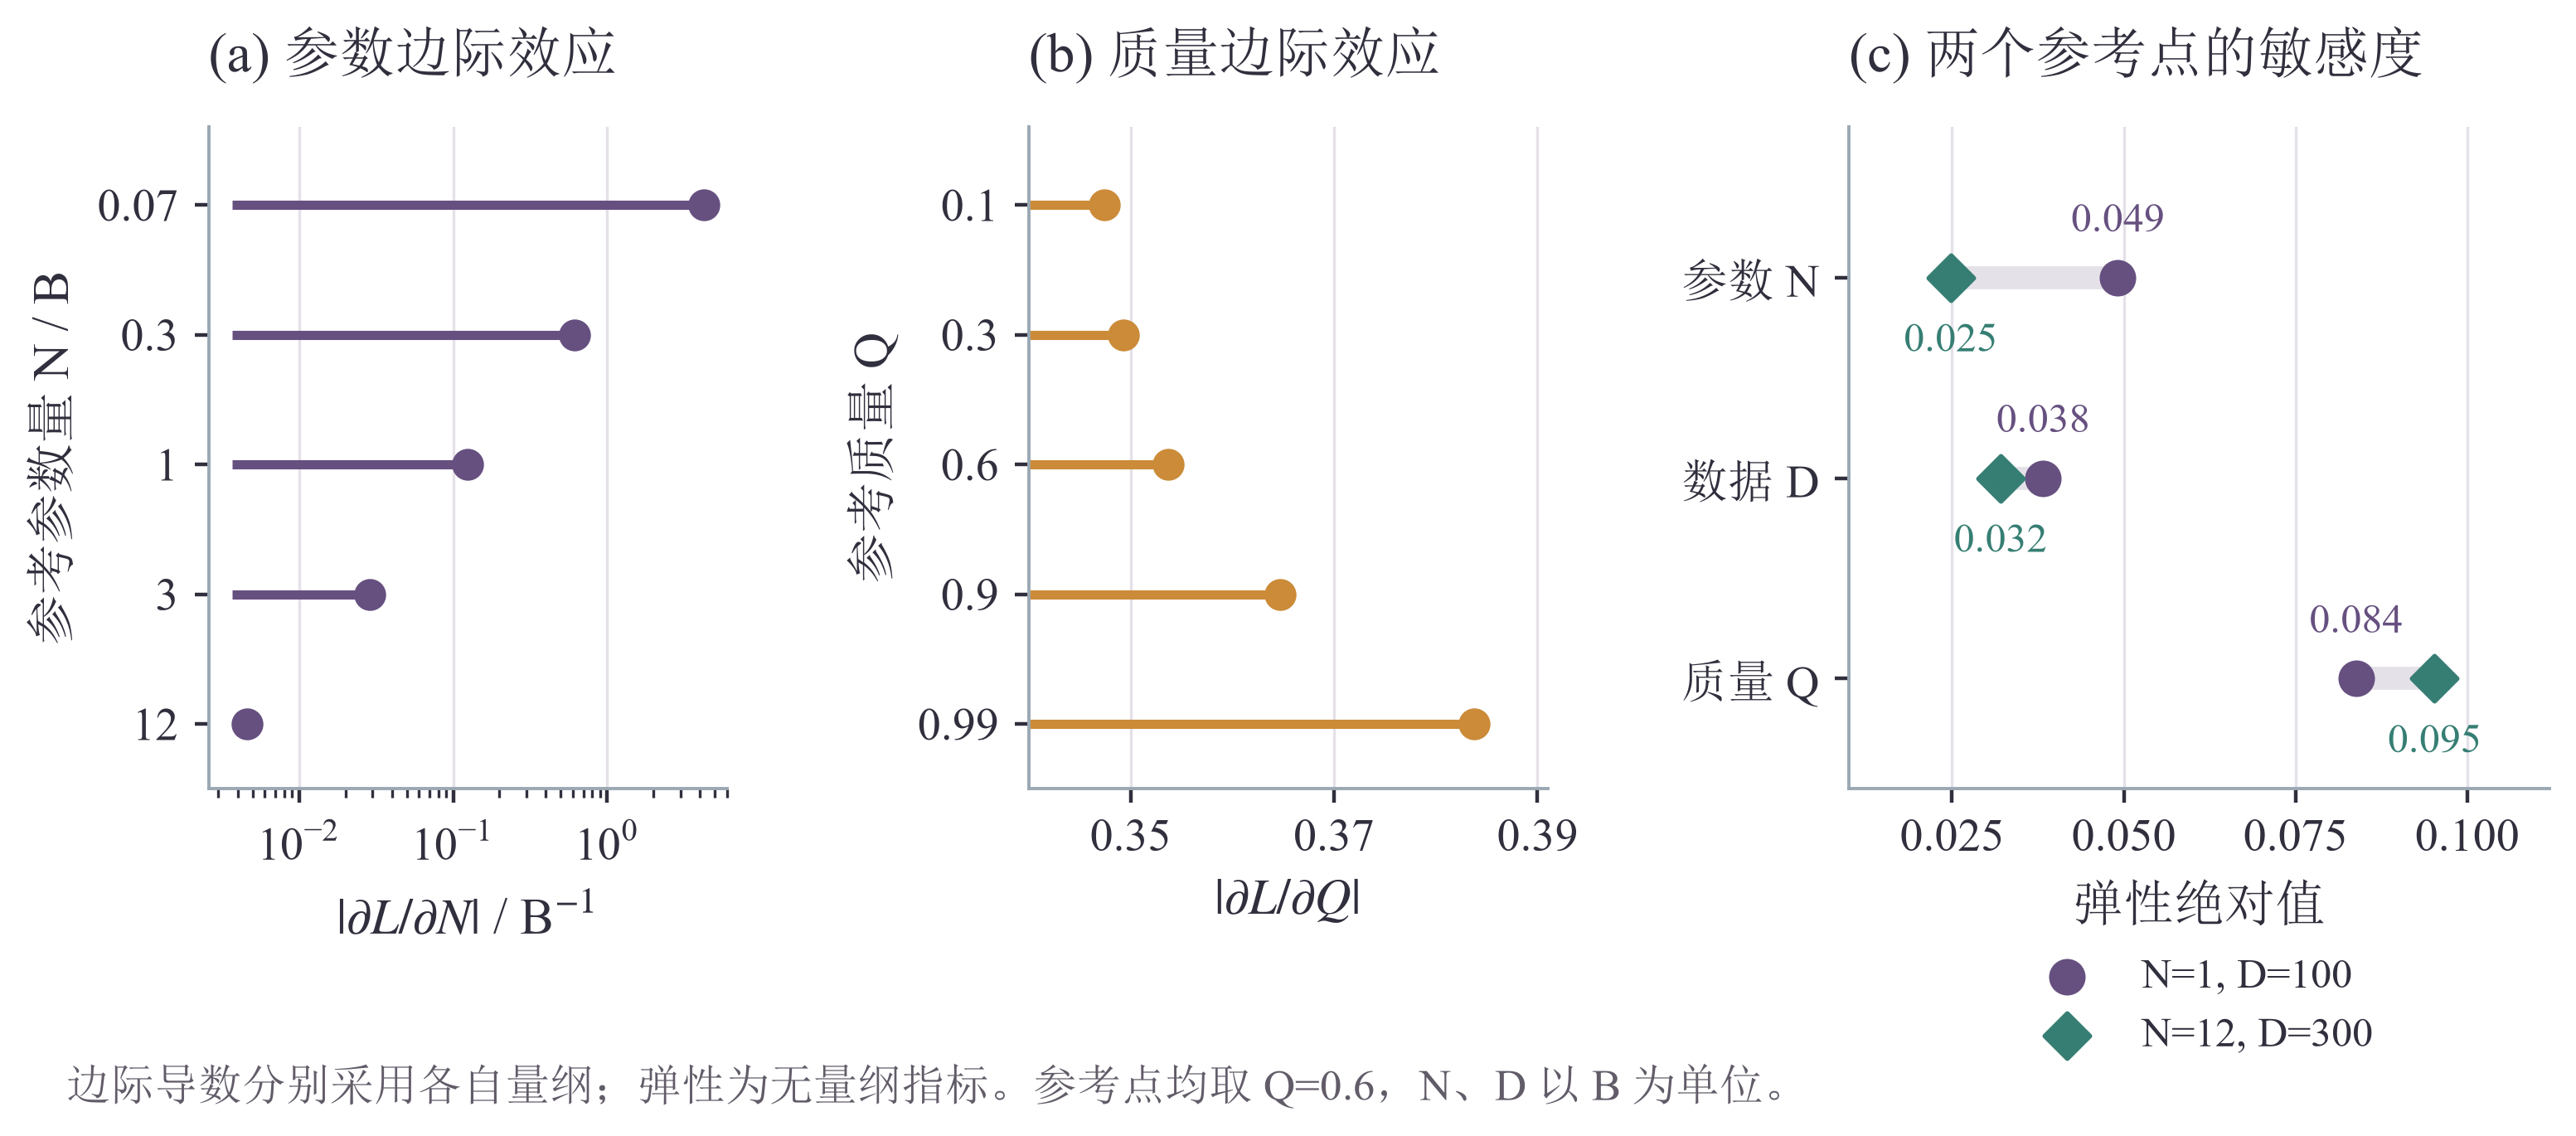
\includegraphics[width=0.98\textwidth]{../求解/问题二/图片/图4_边际效用对比.png}
  \caption{参考位置的边际效应与弹性对比}
  \label{fig:p2_margin}
\end{figure}

\begin{figure}[!htbp]
  \centering
  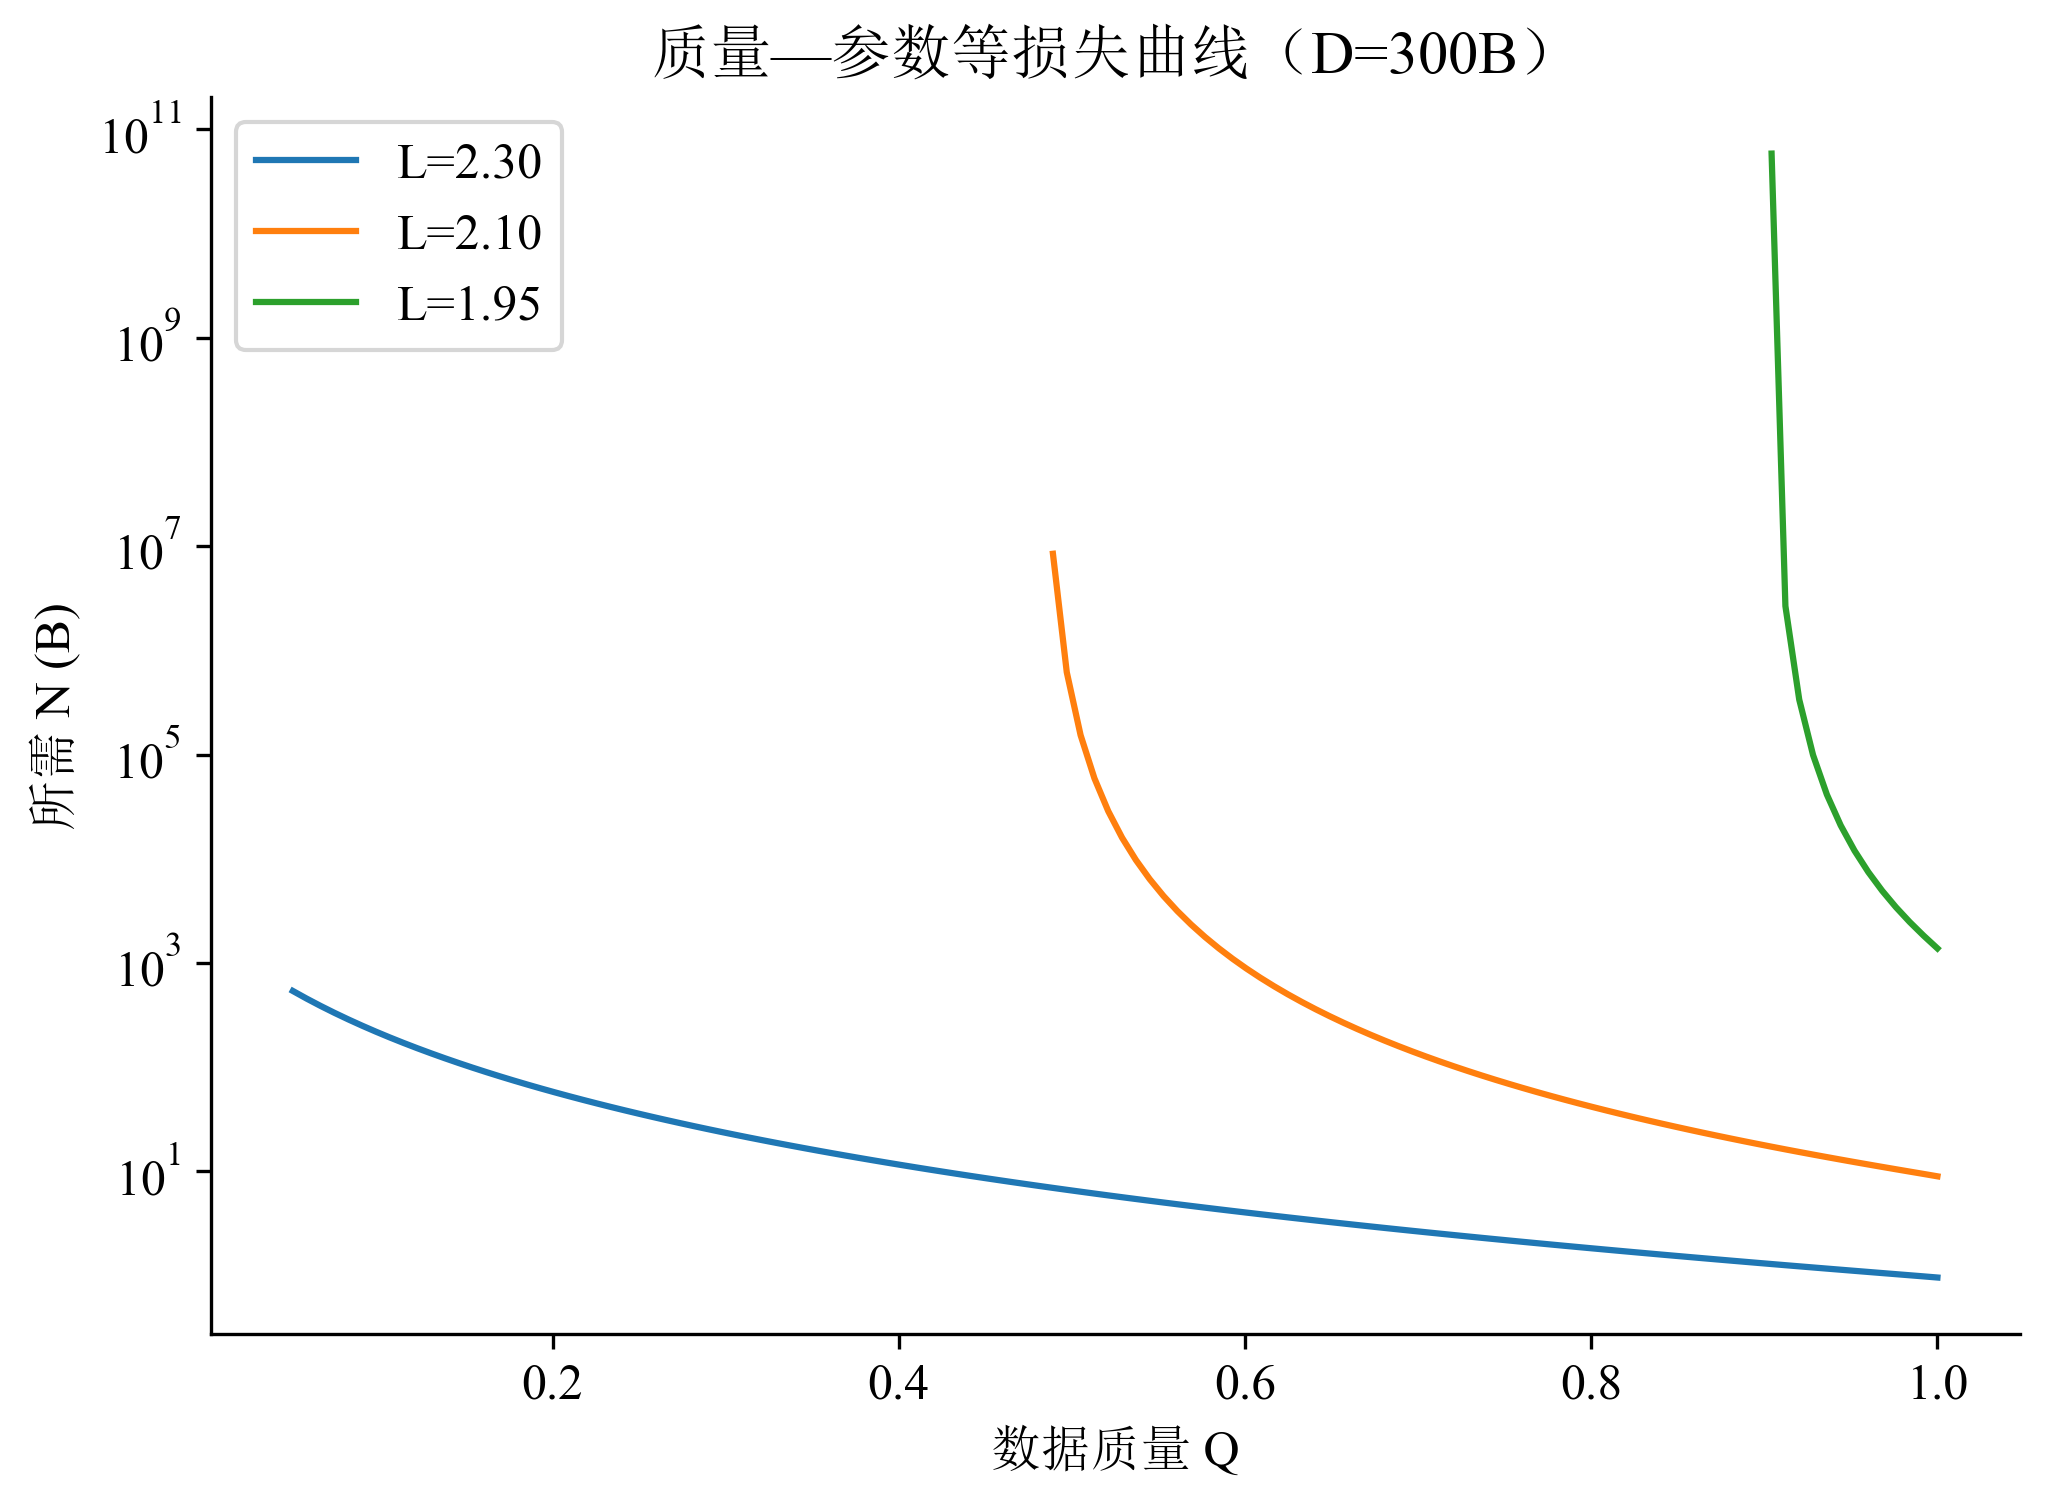
\includegraphics[width=0.98\textwidth]{../求解/问题二/图片/图5_质量参数替代.png}
  \caption{三个目标损失下的规模--质量配置边界}
  \label{fig:p2_subst}
\end{figure}

\begin{samepage}
固定 $D=300$B tokens 后，还可以反求达到目标损失需要的质量，见图\ref{fig:p2_subst}。三个子图各对应一个目标，横轴为参数量，纵轴为质量；实线在主拟合范围内，虚线为外推。对于 $L=1.95$，图中特别放大了高质量区间，并将参数轴延至 $10^4$B 以展示理论边界，这不表示该规模在工程上可行。
\par
\end{samepage}

\begin{samepage}
质量端点需另作处理。估计值 $\gamma=0.9779<1$ 使 $|\partial L/\partial Q|$ 在 $Q<1$ 时逐渐增大，并在 $Q\to1^-$ 时发散。因此，接近质量上界时不能直接用该导数作投入建议，边际效应的数值解释应限于远离端点的位置。
\par
\end{samepage}

\begin{samepage}
\textbf{6.领域效应与配比衔接}\par\nopagebreak[4]
为观察领域之间的关系，图\ref{fig:p2_dom}左侧按 $d_{ij}=\sqrt{2-2s_{ij}}$ 对 17 个训练领域作平均连接聚类；右侧列出相似度最高和最低的各四对领域，用绿色和金色分别表示作用趋同和相反。该图比较的是各域影响验证任务的方式，并不检验混合使用是否产生额外增益。
\par
\end{samepage}

\begin{figure}[!htbp]
  \centering
  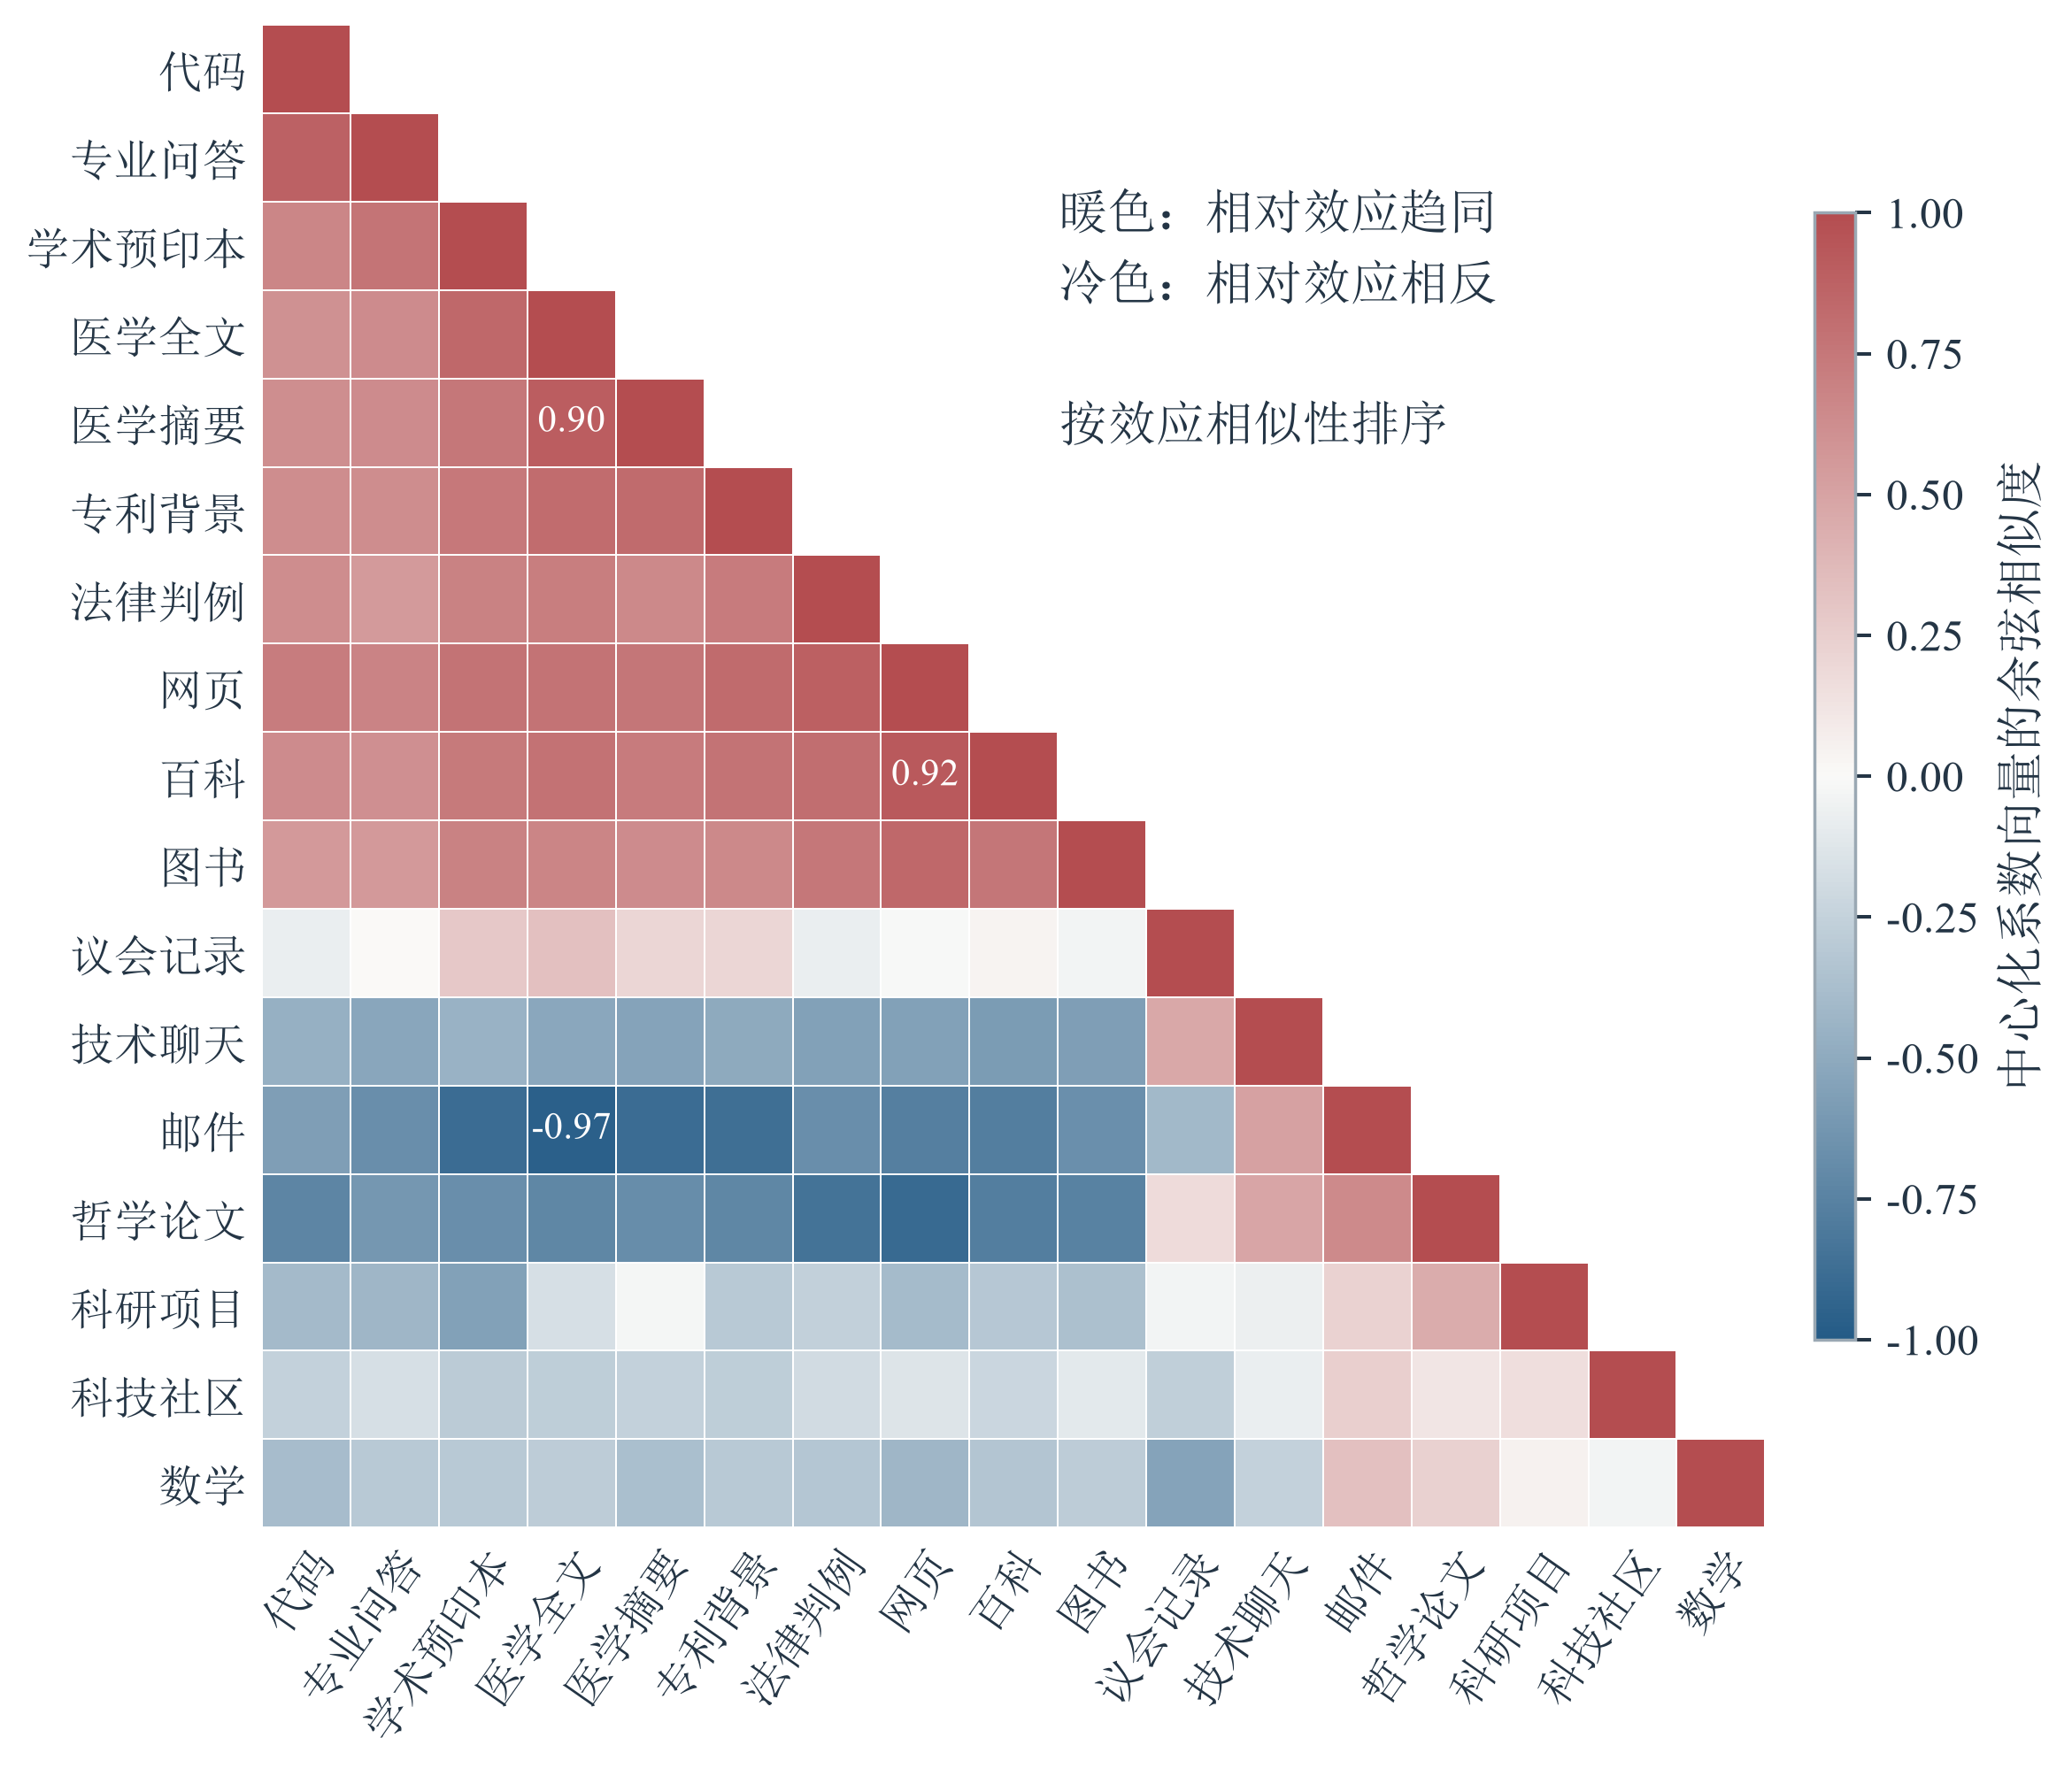
\includegraphics[width=0.98\textwidth]{../求解/问题二/图片/图6_领域替代互补.png}
  \caption{训练领域效应聚类与典型领域对比较}
  \label{fig:p2_dom}
\end{figure}

图\ref{fig:p2_dom}中，百科与网页的相似度为 $0.925$，医学全文与医学摘要为 $0.903$，说明它们在 13 个任务上的相对作用接近；医学全文与邮件为 $-0.967$，表明两者偏向不同任务。若要决定能否替换，还需保留作用大小与任务权重。设从领域 $i$ 向 $j$ 转移占比 $h$，保持总占比不变并满足 $0\leq h\leq p_i$，则预测加权损失变化为
\begin{equation}
  \Delta\widehat L_A=h\,\bm w^{\mathsf T}(\bm a_j-\bm a_i),
\end{equation}
这里 $\bm w$ 是验证领域权重。上式为负时，替换有利于总体表现；为零时效果相当，为正时表现下降。因而，相似度接近并不保证等量替换无损，相反的作用方向也只表示任务之间存在取舍。原模型没有交互项，不能再从中推断两域混合后的额外互补收益。


对问题一推荐配比与参考配比作同口径比较，线性模型给出的加权损失差为
\[
  M=\hat L(\bm p_{\mathrm{rec}})-\hat L(\bm p_{\mathrm{ref}})=-0.1988.
\]
\begin{samepage}
$M$ 来自附件 A 的任务集合和权重。只有在配比效果能够与规模、质量分开，且损失差可在来源之间迁移时，才能将 $M(\bm p)$ 加入广义标度律。前面的检验已显示不同来源存在偏差，所以 $0.1988$ 是当前条件下的损失差，不能保证各个规模都获得同样改善。
\par
\end{samepage}

\begin{samepage}
在上述分离与迁移条件下，规模、质量和配比的关系可合写为
\par\nopagebreak[4]
\begin{equation}
  \begin{aligned}
    L(N,D,Q,\bm p)&=E+AN^{-\alpha}+BD^{-\beta}+C(1-Q)^\gamma+M(\bm p),\\
    M(\bm p)&=\sum_{i=1}^{17}(p_i-p_{\mathrm{ref},i})\,\bm w^{\mathsf T}\bm a_i.
  \end{aligned}
\end{equation}
\end{samepage}
参考配比满足 $M(\bm p_{\mathrm{ref}})=0$。固定配比后，$M$ 只改变损失的整体水平，$N,D,Q$ 的边际导数与等损失替代条件保持不变；本节弹性均在参考配比下计算。若后续直接代入问题一评分，还要假设它与附件 B 的质量尺度能够衔接，这一假设并不能由加性公式自动保证。


本问为预算分配提供了损失函数，也说明了如何使用：模型越大，继续扩参数的边际收益越小；改善质量可以替代多少参数，则取决于初始配置。跨族与文献数据仍有 $8.8\%$、$8.0\%$ 的 MAPE，因此后续配置除了使用拟合值，还需保留对评分尺度、数据来源和外推范围的限制。
\endgroup

\subsection{问题三：算力约束下的资源配置与结构性转移}
\begingroup
\setlength{\tabcolsep}{5pt}

\subsubsection{问题分析与模型准备}

我们在同一训练预算下联合配置参数量、数据量与质量。扩大参数规模会降低参数项损失，同时提高每个 token 的训练费用；改善质量会缩小质量缺口，同时增加整份语料的处理成本。两项投入都会挤占数据训练预算，因此配置时需要比较直接收益与数据量减少带来的损失。

已有研究给出了固定算力下参数和数据的配置关系\cite{hoffmann2022chinchilla}。考虑到题设还包含质量处理与长上下文计算，我们以问题二的损失函数为目标，加入相应费用约束，先求不同预算下的配置，再检验结论对成本形式的依赖。

图\ref{fig:p3_workflow}梳理了本问的计算过程。先汇入前两问的质量基线、配比修正与损失参数，再将训练、质量处理和注意力费用写入预算约束。多初值求解后，分别比较三档预算配置、连续预算中的质量投入阶段，以及成本形式和上下文改变时的配置差异。

\begin{figure}[!htbp]
 \centering
 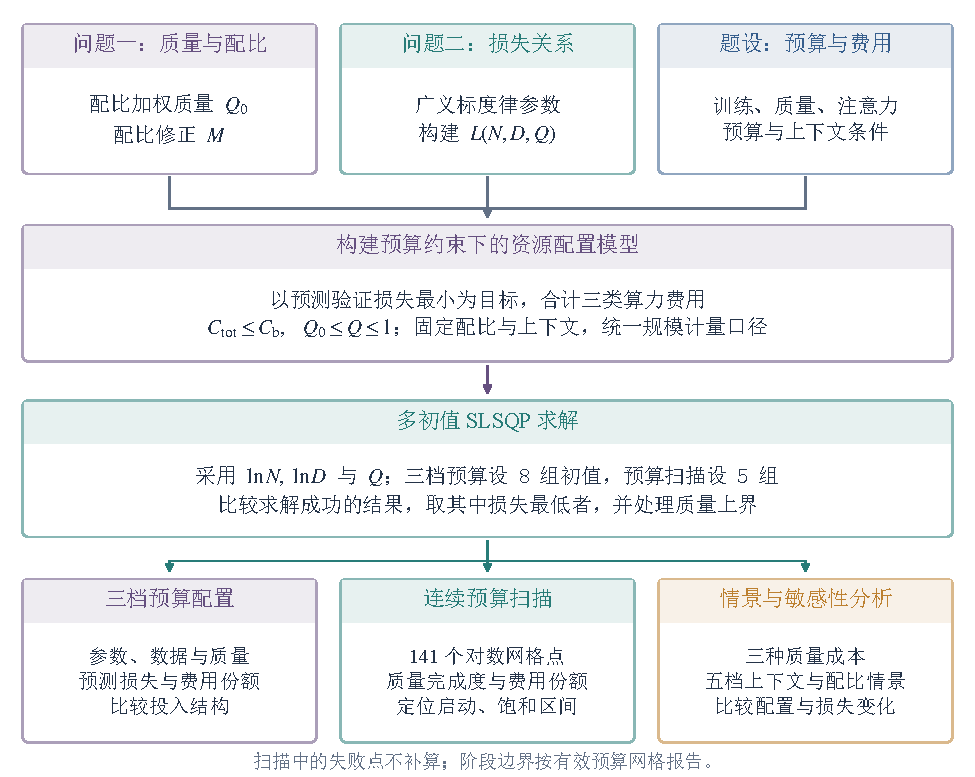
\includegraphics[width=0.94\textwidth]{figures/q3-workflow.pdf}
 \caption{问题三资源配置与求解流程}
 \label{fig:p3_workflow}
\end{figure}

\par\medskip\noindent\textbf{数据与计算口径}\par

本问直接使用问题二估计的损失参数。其中规模项为 $A=0.3808$、$\alpha=0.3266$、$B=1.2515$、$\beta=0.2767$，质量项为 $C_q=0.3544$、$\gamma=0.9779$，常数项为 $E=1.6558$。质量系数改记 $C_q$，以区别预算 $C_{\mathrm b}$。计算费用时，$N$、$D$ 分别用参数个数与 token 个数；代入损失式时再换成 $n=N/10^9$、$d=D/10^9$。下列表格的 B 均表示十亿。

求解器以绝对数量的对数为变量，计算目标和约束时还原规模，再分别用于损失与费用计算。后文的一阶条件也先换算系数，再对绝对数量求导，保持两种计量口径一致。

我们先以参考配方确定质量处理的起点。用 A4 的平均配比 $\bar p_k$ 加权问题一经 A16 映射的领域评分 $Q_k$，得到基线
\[
 Q_0=\sum_{k=1}^{17}\bar p_kQ_k=0.5487.
\]
这里沿用 A4 原始平均份额得到外生成本基线 $Q_0=0.548688$。问题一求核岭配比时将参考份额归一化至和为 1，其加权质量为 0.548753；两种口径分别记录，不因配比归一化而重设本问的费用起点。全量文本均值 $0.4912$ 另作灵敏度对照。

记问题一评分为 $Q_A$、附件 B 评分为 $Q_B$，本问采用 $Q_B=h(Q_A)=Q_A$，并在共同数值轴上计算费用。恒等映射是缺少配对标定资料时的情景假设。优化范围为 $Q_0\le Q\le1$，满分只表示模型质量上界。

配比比较保持共同 $Q_0$，只对超过该基线的质量计费。核岭候选自身的加权质量为 0.5182，换配方后原料质量并不相同。若按各配方质量 $Q_0(\bm p)$ 分别计费，就需要另行求解配比与处理成本的耦合；本节先单独比较固定损失平移，随后给出更换费用基线的对照。

基准情景取参考配比 $M=0$、幂函数成本及 $2048$ tokens 上下文；成本类型和上下文依次改变。附件 C7 的 2048、4096、8192、32768、131072 tokens 均作为给定条件，求解器只调整参数、数据与质量。此外，将核岭配比对应的 $M=-0.1730$ 单列为收益情景，检查损失与等效预算如何变化。

\subsubsection{模型建立}

\textbf{1.每个训练 token 的算力代价}\par\nopagebreak[4]
基础训练使用 $6ND$ 的成本近似\cite{hoffmann2022chinchilla}，质量与注意力费用按照题目第三问及题目附录 B 的成本设定计算。由于三类 $g(Q)$ 在允许范围内均递增，可记质量提升的单位增量费用为 $\Delta g(Q)=g(Q)-g(Q_0)\ge0$，从而将总成本写为
\begin{equation}
 C_{\mathrm{tot}}
 =6ND+D\Delta g(Q)+\eta ND L_{\mathrm{ctx}}
 =D\underbrace{\left[(6+\eta L_{\mathrm{ctx}})N+\Delta g(Q)\right]}_{\text{单位 token 的合计算力成本}},
 \qquad \eta=2\times10^{-4}.
 \label{eq:p3_cost_total}
\end{equation}
三项费用都随数据量 $D$ 累计。给定 $N,Q$ 时，每个新增 token 的单价不变；提高质量则增加整份语料的处理费用，压缩可用于训练的数据量。即使质量已达上界，新增数据仍需支付处理费用。

这里的 $D$ 按累计训练 token 数使用，质量费用也按相同数量核算，尚未扣除重复使用语料可能带来的处理成本复用。若一份语料仅预处理一次、随后多轮训练，应区分独立语料量与累计训练量；当前算例沿用题设费用，不对这类复用作额外修正。

表\ref{tab:p3_functions}列出题设的三种质量成本。由于比较的是相对基线的增量 $\Delta g(Q)$，三种函数在 $Q_0$ 处均不产生额外费用。
\begin{table}[htbp]
 \centering
 \normalfont\normalsize\color{black}
 \renewcommand{\arraystretch}{1.15}
 \caption{质量处理成本函数（$g$ 的单位为 FLOPs/token）}
 \label{tab:p3_functions}
 \begin{tabularx}{0.98\textwidth}{@{}*{3}{>{\centering\arraybackslash}X}@{}}
 \toprule
 成本类型 & $g(Q)$ & 本节用途\\
 \midrule
 幂函数型 & $5\times10^9Q^4$ & 基准配置\\
 指数型 & $10^7e^{6Q}$ & 成本形式对照\\
 对数渐进型 & $2\times10^9\ln(1+10Q)$ & 成本形式对照\\
 \bottomrule
 \end{tabularx}
\end{table}

\textbf{2.预算约束下的配置模型}\par\nopagebreak[4]
记 $k=6+\eta L_{\mathrm{ctx}}$。给定配比和上下文长度后，以预测验证损失最小为目标，得到
\begin{equation}
 \begin{aligned}
 \min_{N,D,Q}\quad &E+A n^{-\alpha}+B d^{-\beta}+C_q(1-Q)^\gamma+M,\\
 \mathrm{s.t.}\quad&D\,[kN+\Delta g(Q)]\le C_{\mathrm b},\qquad Q_0\le Q\le1,\\
 &10^5\le N\le10^{15},\qquad 10^6\le D\le10^{16}.
 \end{aligned}
 \label{eq:p3_problem}
\end{equation}
末尾界限限定数值搜索范围，不代表实际数据供给。共同 $Q_0$ 固定、配比可行域独立且 $M(\bm p)$ 可加分离时，先最小化 $M$ 再优化 $N,D,Q$，与联合最小化等价；若基线或费用随配比变化，这种分离便不再成立。本文使用问题一多初值求得的核岭候选，不据此保证全局最优或真实训练收益。因此，“配比改变而配置不变”来自模型设定。

固定质量且规模界限不活跃时，增加 $N$ 或 $D$ 都能降低损失，预算约束因而取等号。将其写为
\begin{equation}
 D=\frac{C_{\mathrm b}}{kN+\Delta g(Q)}
 \label{eq:p3_budget_balance}
\end{equation}
预算式说明，提高 $N$ 或 $Q$ 后，能够负担的 $D$ 都会减少。因此，我们比较一项投入的净收益时，同时计入其直接降低的损失与数据缩减增加的损失。

预算用尽可由数据项的单调性说明：在 $N,Q$ 固定、数据上界未达到时，增加 $D$ 只会减小 $Bd^{-\beta}$。若仍有余款，就还可降低损失。消去数据量后，可在预算边界上比较参数与质量；以下用该化简解释一阶条件，正式程序仍求解三变量约束模型。

由式\eqref{eq:p3_budget_balance}还可分别求得预算固定时的数据变化：
\begin{equation}
 \left.\frac{\partial D}{\partial N}\right|_Q
 =-\frac{kD}{kN+\Delta g(Q)},\qquad
 \left.\frac{\partial D}{\partial Q}\right|_N
 =-\frac{Dg'(Q)}{kN+\Delta g(Q)}.
 \label{q3_expand_data_tradeoff}
\end{equation}
两项均为负，分别对应扩大模型和提高质量带来的数据缩减。质量成本的影响还取决于当前位置的斜率 $g'(Q)$，因而不能只比较不同成本函数在某一个质量水平上的取值。这也说明，费用形式相近的情景仍可能产生不同的质量选择。

\textbf{3.参数量与数据量的平衡}\par\nopagebreak[4]
为统一求导单位，先令 $\widetilde A=A(10^9)^\alpha$、$\widetilde B=B(10^9)^\beta$，把规模项改写为绝对数量形式。固定 $Q$ 后，将预算等式\eqref{eq:p3_budget_balance}代入损失函数，可得
\[
 F(N)=\widetilde A N^{-\alpha}
      +\widetilde B\left[\frac{kN+\Delta g(Q)}{C_{\mathrm b}}\right]^\beta.
\]
此处省略的常数项和质量项在固定质量后不随 $N$ 变化，不影响导数。参数项的导数为负，数据项则因预算挤占而产生正导数，两者相加为
\begin{equation}
 F'(N)=-\alpha\widetilde A N^{-\alpha-1}
 +\frac{\beta\widetilde Bk}{C_{\mathrm b}^{\beta}}
       [kN+\Delta g(Q)]^{\beta-1}.
 \label{q3_expand_parameter_derivative}
\end{equation}
令该式为零，再乘以 $[kN+\Delta g(Q)]/k$，并用预算等式替换数据项，即可得到参数与数据损失的平衡关系。
对应的平衡式为
\begin{equation}
 \alpha\widetilde A N^{-\alpha}
 \left(1+\frac{\tau(Q)}{N}\right)
 =\beta\widetilde B D^{-\beta},
 \qquad \tau(Q)=\frac{\Delta g(Q)}k.
 \label{eq:p3_balance}
\end{equation}
为解释式\eqref{eq:p3_balance}，可把 $\tau(Q)$ 看作质量费用折算出的附加参数规模，它与 $N$ 单位相同。因而，因子 $1+\tau/N$ 表示额外质量处理对规模平衡的影响。一旦为质量付费，原本只在参数与数据之间分配的方案就需要随之调整。

作为对照，保持基线质量时有 $\tau=0$，于是 $\alpha\widetilde A N^{-\alpha}=\beta\widetilde B D^{-\beta}$。将其与 $kND=C_{\mathrm b}$ 联立，在上下文固定时得到
\begin{equation}
 N^*\propto C_{\mathrm b}^{\beta/(\alpha+\beta)},\qquad
 D^*\propto C_{\mathrm b}^{\alpha/(\alpha+\beta)}.
 \label{eq:p3_scaling}
\end{equation}
不额外提高质量时，数据量随预算增长稍快于参数量：两者的指数分别约为 $0.541$、$0.459$。这只是基线质量下的参照；开始投入质量后，应回到包含处理费用的完整模型计算。

基线幂律的比例系数也可由同一组方程求出。将 $D=C_{\mathrm b}/(kN)$ 代入平衡条件，得到
\begin{equation}
 \begin{aligned}
 (N^*)^{\alpha+\beta}
 &=\frac{\alpha\widetilde A}{\beta\widetilde B}
   \left(\frac{C_{\mathrm b}}{k}\right)^\beta,\\
 N^*&=\left(\frac{\alpha\widetilde A}{\beta\widetilde B}\right)^{1/(\alpha+\beta)}
       \left(\frac{C_{\mathrm b}}{k}\right)^{\beta/(\alpha+\beta)},\\
 D^*&=\left(\frac{\beta\widetilde B}{\alpha\widetilde A}\right)^{1/(\alpha+\beta)}
       \left(\frac{C_{\mathrm b}}{k}\right)^{\alpha/(\alpha+\beta)}.
 \end{aligned}
 \label{q3_expand_baseline_closed_form}
\end{equation}
因此，预算通过幂指数决定规模的增长速度，系数比值决定具体配置水平。上下文固定时，$k$ 只进入有效预算因子；质量费用不为零时，预算中多出无法并入 $kN$ 的处理项，基线表达式便不再适用于完整配置。因此，该解析式只适用于没有质量增量费用的参照情形，用来解释规模权衡；完整配置仍由含质量费用的预算模型求解。

质量选择也可在同一预算边界上解释。当预算约束活跃、数据量未触及搜索上下界且 $Q_0<Q<1$ 时，固定 $N$ 并对消去数据量后的损失求导，质量最优的必要条件为
\begin{equation}
 \frac{\beta\widetilde B D^{-\beta}g'(Q)}{kN+\Delta g(Q)}
 =\gamma C_q(1-Q)^{\gamma-1}.
 \label{q3_expand_quality_balance}
\end{equation}
式中左侧是质量提升挤占数据预算后增加的损失，右侧是质量改善直接减少的损失。我们据此将内部配置解释为两项边际作用相抵的结果。若解位于基线或质量上界，应结合允许的变化方向判断，不能要求上述等式成立。尤其在上界处，质量项的导数性质与内部不同。因此，本问的阶段位置仍依据后文的预算扫描确定，一阶条件用于解释内部配置的局部权衡。

\textbf{评分尺度的条件对照。} 为检查恒等映射的影响，我们保留 $Q_A$ 轴上的幂函数费用，分别令 $Q_B=h(Q_A)$ 取 $\sqrt{Q_A}$、$Q_A$、$Q_A^2$。三者方向及端点相同，但固定 $N,D$ 时，质量项关于处理评分的损失导数变为
\begin{equation}
 -\frac{\partial L}{\partial Q_A}
 =C_q\gamma[1-h(Q_A)]^{\gamma-1}h'(Q_A).
 \label{eq:q23_review_quality_mapping}
\end{equation}
在参考配比、2048 tokens 上下文及基线规模最优曲线上，以质量收益与预算挤占损失的一阶平衡确定下界释放点，得到表\ref{tab:q23_review_quality_scale}。该点说明何时从基线小幅提高质量开始有利，存在竞争端点时不一定等于全局阶段边界。

\begin{table}[htbp]
 \centering
 \caption{评分映射改变时的局部质量投入释放点}
 \label{tab:q23_review_quality_scale}
 \renewcommand{\arraystretch}{1.15}
 \begin{tabularx}{0.94\textwidth}{@{}*{3}{>{\centering\arraybackslash}X}@{}}
 \toprule
 映射 $h(Q_A)$ & 参考基线在 B 轴的值 & 释放预算（$10^{19}$ FLOPs） \\
 \midrule
 $\sqrt{Q_A}$ & 0.7407 & 2.94 \\
 $Q_A$ & 0.5487 & 1.57 \\
 $Q_A^2$ & 0.3011 & 1.37 \\
 \bottomrule
 \end{tabularx}
\end{table}

这些映射用于检验同向评分并不唯一决定投入阈值，没有被当作新的标定结果。基准情景仍用恒等映射；其他处理评分或实际费用若定义在不同尺度上，应先同步转换损失与费用，再使用相应配置。

\textbf{4.数值求解与阶段识别}\par\nopagebreak[4]
我们采用 SciPy 的 SLSQP 实现\cite{scipy_slsqp}求解式\eqref{eq:p3_problem}，以 $\ln N$、$\ln D$ 缩小变量尺度差异，并将预算不等式等价写为 $1-C_{\rm total}/C_{\mathrm b}\ge0$，避免约束绝对量级过大；停止条件取 ftol=$10^{-14}$，单次求解最多迭代 1500 次。三档预算各设 8 组初值，连续预算扫描各设 5 组，从求解成功的结果中选取损失最低的一组，记作 $(N^*,D^*,Q^*)$。这样可降低初值和局部解的影响，但不能保证全局最优。另因 $\gamma<1$ 时 $Q=1$ 的导数无界，将达到该上界的配置作为边界解处理。将保存的配置重新代入成本函数，三档预算、上下文敏感性与全部 141 个预算扫描点的最大相对预算残差均小于 $10^{-12}$。这些数值核验说明记录的配置满足预算约束，但只验证可行性，不构成对全局最优性的证明。

对数变量使参数量与数据量的正值约束自然满足，原有规模上下界相应转换为对数区间。实际初值设置让参数量与数据量沿相反方向变化，同时使质量起点分布在允许区间内部，以比较不同资源组合出发后的求解结果。每次求解都保留总预算不等式和质量边界，而不是先独立确定三项投入后再缩放预算。成功状态用于筛选候选结果，边界配置则保留其实际质量值；未记录成功结果的预算点不参与后续阶段定位。多初值比较用于同一预算下的候选选择，相邻预算点仍分别求解，阶段变化依据有效输出识别。

质量投入的阶段用完成度 $\Theta=(Q^*-Q_0)/(1-Q_0)$ 表示，质量处理占预算的份额用 $f_Q=D^*\Delta g(Q^*)/C_{\mathrm b}$ 表示。完成度为 0 时维持基线，介于 0、1 时正在提升，等于 1 时达到上界。计算在 $10^{18}$--$10^{25}$ FLOPs 内设置 141 个对数等距点，相邻预算之比约为 1.122，逐点寻找首次投入与首次饱和的位置。采用无量纲预算约束后，141 个网格点均取得有效配置，阶段分析使用全部输出。

我们同时观察完成度与费用份额，以区分质量提升的进度和资源支出。前者以可提升的质量区间为分母，后者以总预算为分母；质量不变时，规模调整仍可能改变费用份额。因此，质量曲线变平不表示处理费用消失，阶段位置也只能由有效预算网格点定位。

\subsubsection{模型求解}

图中坐标、费用份额及网格判定的计算口径见附录 F。

\noindent\textbf{辅助分析说明：} 本问的文段相关辅助参考腾讯 WorkBuddy 接入的 DeepSeek-V4-Flash（2026-07-31 公开测试），图表展示、程序整理与复现核对使用 OpenAI Codex（GPT-5.6-Luna，2026-07-09）\cite{ai_workbuddy,ai_deepseek,ai_codex56luna}。正文表达与段落衔接另经 OpenAI Codex 辅助润色。

\textbf{1.预算增加后，质量与规模如何分配}\par\nopagebreak[4]
比较表\ref{tab:p3_opt}中的三档配置，我们发现各项投入并未按相同比例增长。参数和数据都在增加，但数据更快，$D/N$ 由 30.9 升到 76.1。质量在低预算档停留于基线，中、高预算档则达到上界，不能简单地按固定比例同时扩张三项投入。

\begin{table}[htbp]
 \centering
 \normalfont\normalsize\color{black}
 \renewcommand{\arraystretch}{1.15}
 \caption{三档预算的基准配置（幂函数型成本，$L_{\mathrm{ctx}}=2048$，$M=0$）}
 \label{tab:p3_opt}
 \begin{tabularx}{0.98\textwidth}{@{}*{7}{>{\centering\arraybackslash}X}@{}}
 \toprule
 \makecell{预算\\（FLOPs）} & $N^*$（B） & \makecell{$D^*$\\（B tokens）} & $Q^*$ & $L^*$ & $D^*/N^*$ & $f_Q$（\%）\\
 \midrule
 $10^{19}$ & 0.225 & 6.9 & 0.549 & 3.171 & 30.9 & 0.0 \\
 $10^{22}$ & 6.091 & 229.4 & 1.000 & 2.145 & 37.7 & 10.4 \\
 $10^{24}$ & 44.939 & 3417.8 & 1.000 & 1.897 & 76.1 & 1.6 \\
\bottomrule
 \end{tabularx}
\end{table}

为定位质量投入的阶段变化，我们继续沿用幂函数型成本、$L_{\mathrm{ctx}}=2048$、$M=0$ 作预算扫描。图\ref{fig:p3_shift}左侧为完成度，右侧为三类费用份额，内嵌小图放大了质量提升区间。两条竖线对应首次启动和首次饱和的有效网格点；曲线连接逐点求解得到的记录。
\begin{figure}[htbp]
 \centering
 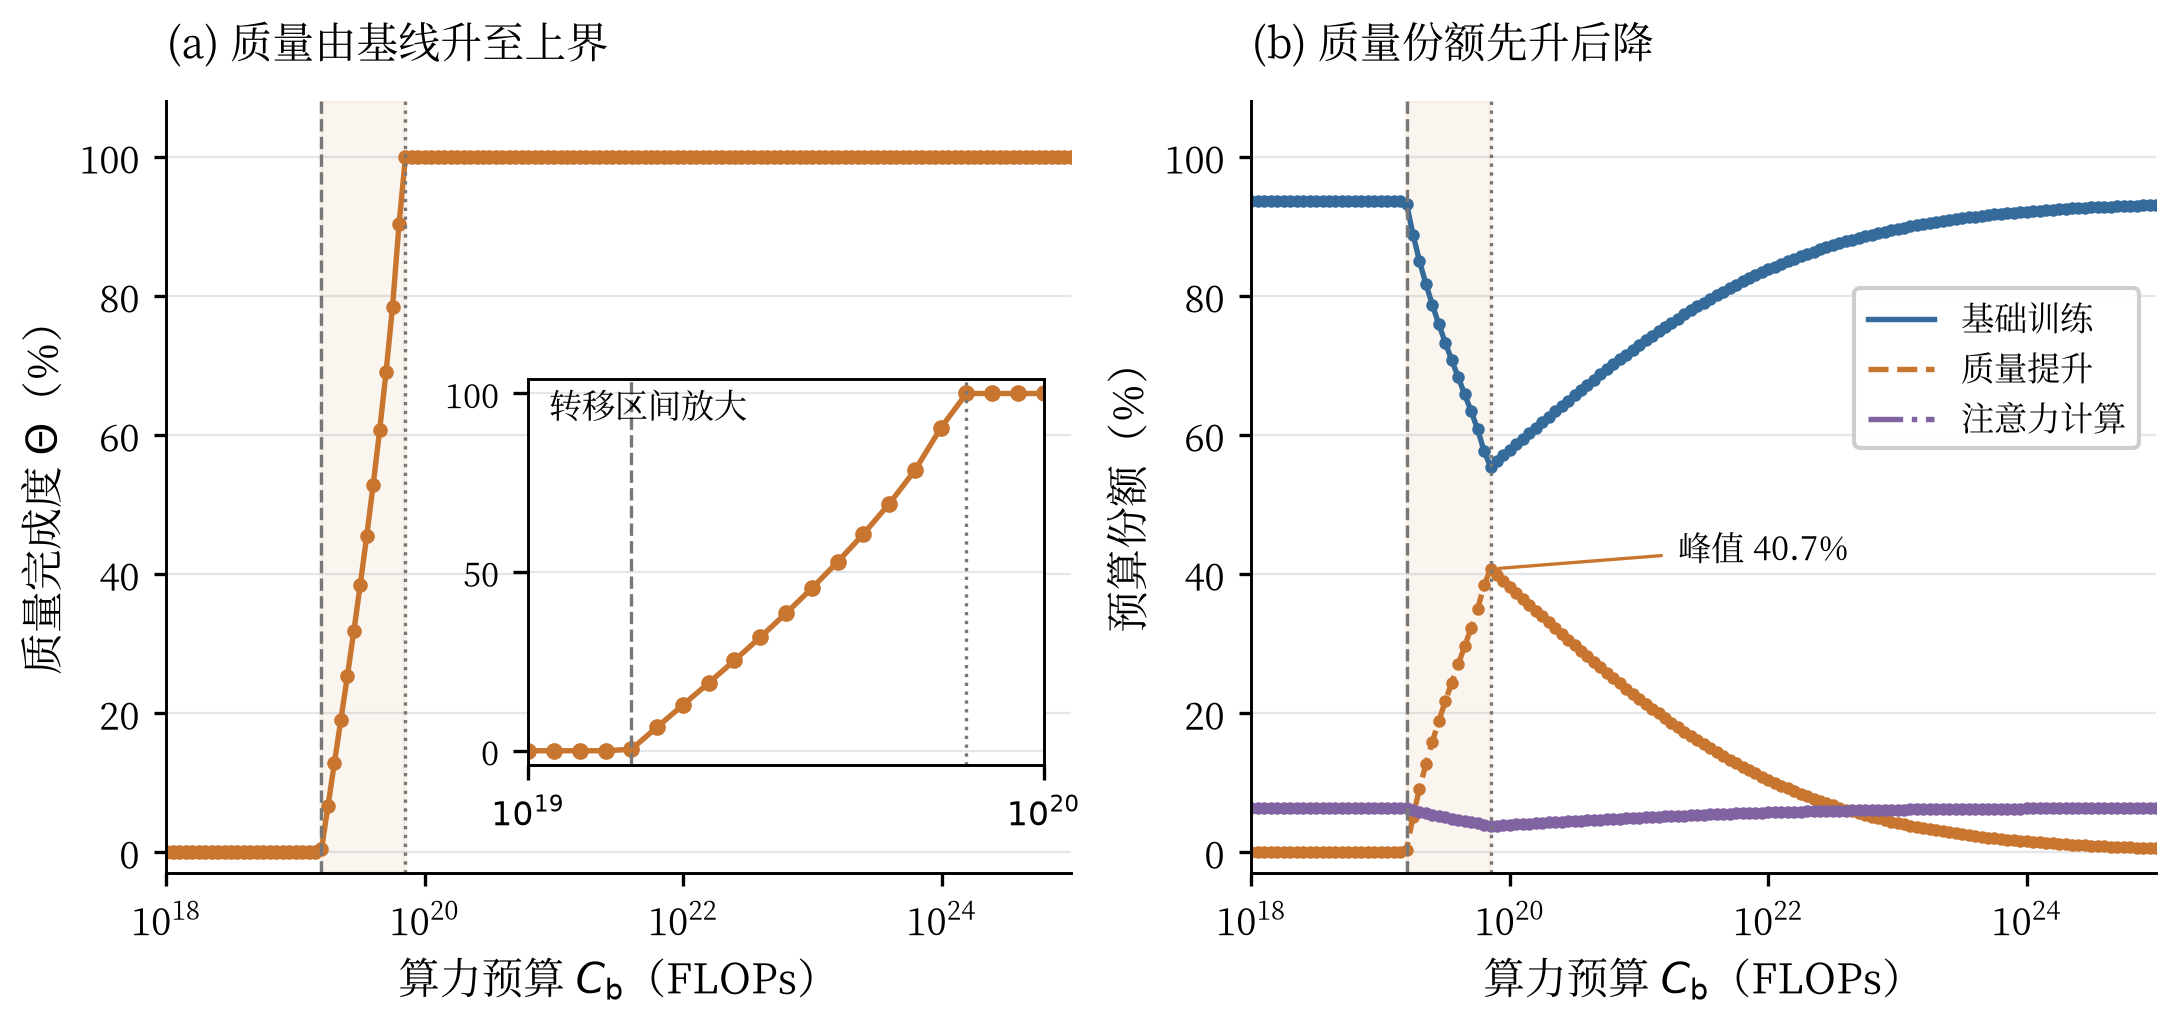
\includegraphics[width=0.94\textwidth]{../求解/问题三/图片/图2_预算份额结构性转移.png}
 \caption{给定标度律参数下的预算与费用份额}
 \label{fig:p3_shift}
\end{figure}

低预算的有效解都保持 $Q^*=Q_0$。此时 $93.6\%$ 用于基础训练，$6.4\%$ 用于注意力计算。虽然提高质量可降低质量项损失，但它会占用原本可用于数据训练的费用；在当前成本设定下，数值比较选择维持基线。

费用份额的变化可进一步从预算等式得到解释。记基础训练和注意力的份额分别为 $f_{\mathrm{train}}$、$f_{\mathrm{attn}}$，预算充分使用时有
\begin{equation}
 f_{\mathrm{train}}=\frac{6N^*}{kN^*+\Delta g(Q^*)},\qquad
 f_{\mathrm{attn}}=\frac{\eta L_{\mathrm{ctx}}N^*}{kN^*+\Delta g(Q^*)},\qquad
 f_{\mathrm{train}}+f_{\mathrm{attn}}+f_Q=1.
 \label{q3_expand_budget_shares}
\end{equation}
上下文固定时，基础训练与注意力的费用比保持不变。质量投入出现后，这两项在总预算中的份额会共同受到压缩，但彼此的比例仍由上下文决定。因此，图中的三类份额并非能够任意调整的三个独立变量，其变化受到成本结构的约束。

质量投入的两个变化位置可以从扫描点看出。到 $1.58\times10^{19}$ FLOPs，首次出现额外质量费用；到 $7.08\times10^{19}$ FLOPs，质量达到上界，费用份额也升至峰值 $40.7\%$。在后一位置之前，最近有效点的质量约为 0.956。结合相邻点，启动区间为 $[1.41,1.58]\times10^{19}$ FLOPs，饱和区间为 $[6.31,7.08]\times10^{19}$ FLOPs。这些是当前网格的定位范围，精确临界值并未由扫描确定。

上述区间仅反映原参数和当前网格。表\ref{tab:q23_review_gamma}中，$\gamma=1$ 的受限拟合与原拟合目标接近，却使原首次饱和点的质量变为 0.9640，说明网格定位误差之外还存在函数形状的不确定性。因此，三阶段图用于解释现有情景，不将两个网格区间当作已经验证稳健的投入门槛。

达到质量上界后，$Q$ 已不能继续增加，新增预算主要用于扩参数和数据。此时单位质量费用固定为 $\Delta g(1)$，预算关系给出
\[
 f_Q=\frac{\Delta g(1)}{kN^*+\Delta g(1)}.
\]
达到上界后，模型越大，质量费用份额越小，至 $10^{24}$ FLOPs 约为 $1.6\%$。这是训练费用增长更快造成的，不能理解为质量处理总支出减少，因为每个新增 token 仍承担同样的处理费用。质量不再增加也来自上界约束，而非边际收益归零；问题二估计的 $\gamma$ 仍小于 1。

\FloatBarrier

\textbf{2.低预算的质量选择取决于成本形式}\par\nopagebreak[4]
我们进一步更换质量成本形式，检查上述阶段是否依赖幂函数设定。保持 $L_{\mathrm{ctx}}=2048$、$M=0$，用表\ref{tab:p3_functions}的三种函数分别求解。图\ref{fig:p3_cost}对照九组结果的质量及费用份额，表\ref{tab:p3_cost}列出对应规模配置。
\begin{figure}[htbp]
 \centering
 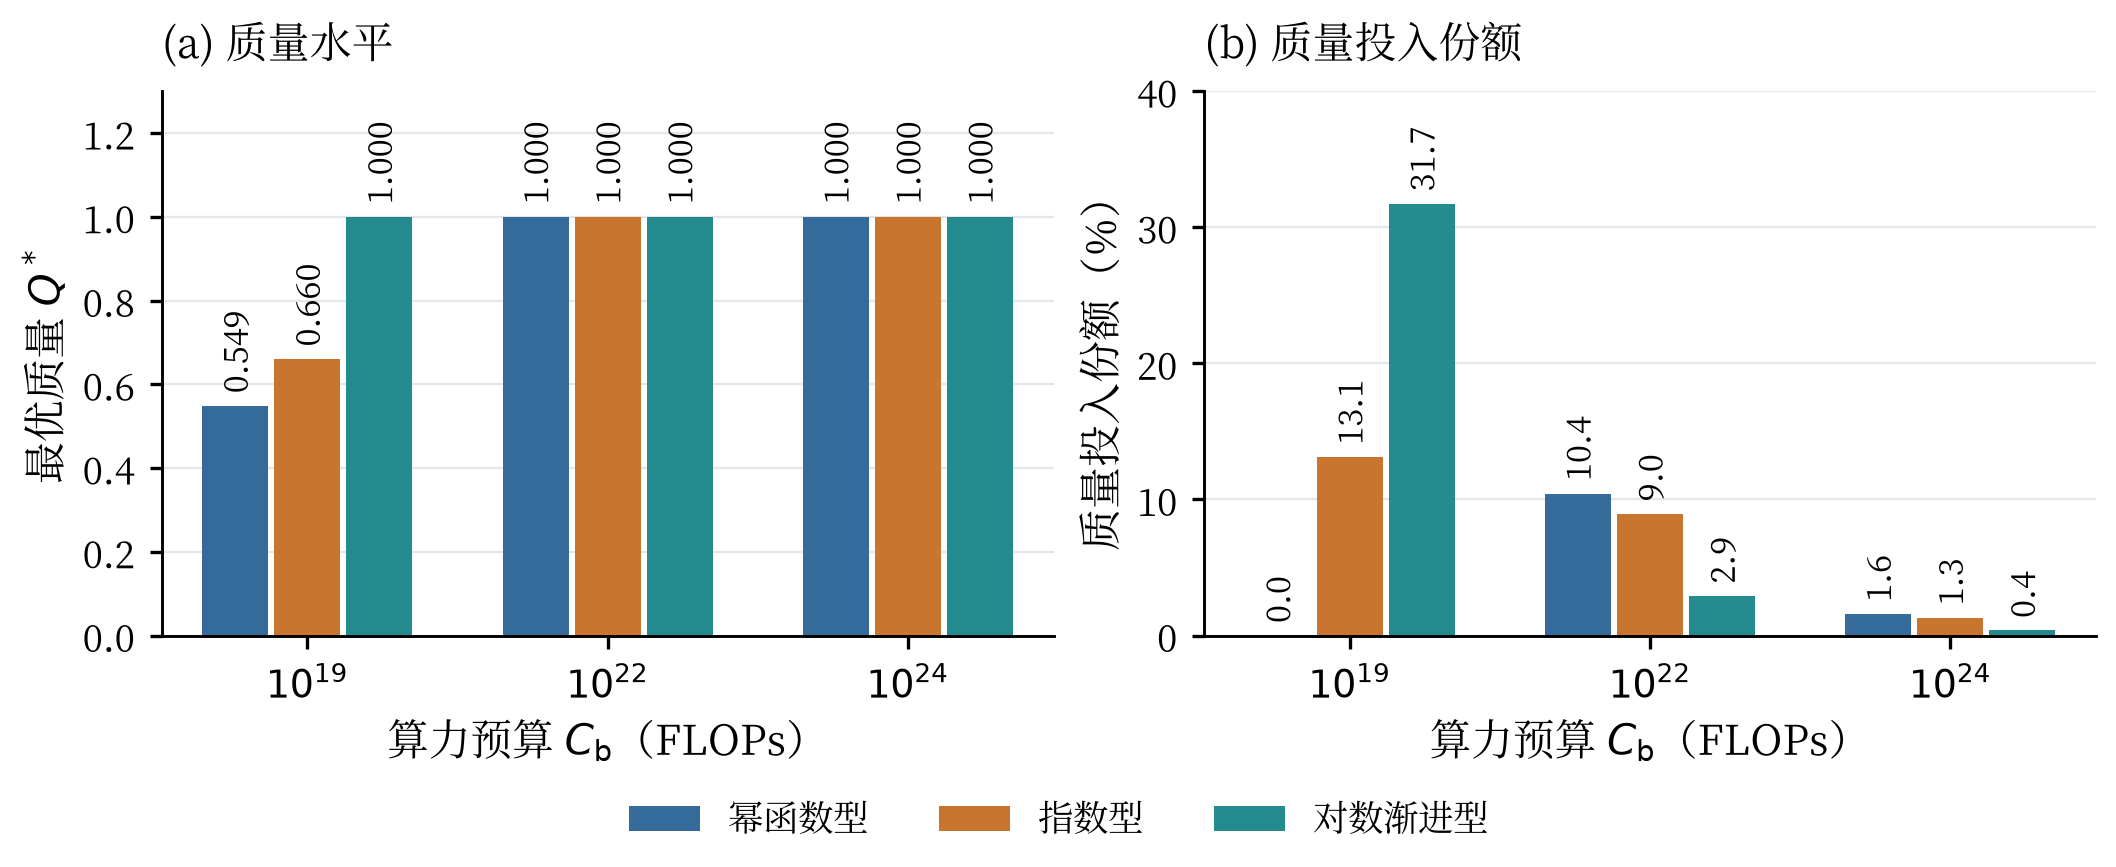
\includegraphics[width=0.94\textwidth]{../求解/问题三/图片/图4_质量成本函数对比.png}
 \caption{成本函数比较}
 \label{fig:p3_cost}
\end{figure}

\begin{table}[htbp]
 \centering
 \normalfont\normalsize\color{black}
 \renewcommand{\arraystretch}{1.15}
 \caption{三类质量成本下的配置对比（$L_{\mathrm{ctx}}=2048$，$M=0$）}
 \label{tab:p3_cost}
 \begin{tabularx}{0.98\textwidth}{@{}>{\hsize=0.95\hsize\linewidth=\hsize\centering\arraybackslash}X>{\hsize=1.4\hsize\linewidth=\hsize\centering\arraybackslash}X>{\hsize=0.93\hsize\linewidth=\hsize\centering\arraybackslash}X>{\hsize=0.93\hsize\linewidth=\hsize\centering\arraybackslash}X>{\hsize=0.93\hsize\linewidth=\hsize\centering\arraybackslash}X>{\hsize=0.93\hsize\linewidth=\hsize\centering\arraybackslash}X>{\hsize=0.93\hsize\linewidth=\hsize\centering\arraybackslash}X@{}}
 \toprule
 \makecell{预算\\（FLOPs）} & 成本类型 & $N^*$（B） & \makecell{$D^*$\\（B tokens）} & $Q^*$ & $L^*$ & $f_Q$（\%）\\
 \midrule
 $10^{19}$ & 指数型 & 0.266 & 5.1 & 0.660 & 3.163 & 13.1 \\
  & 幂函数型 & 0.225 & 6.9 & 0.549 & 3.171 & 0.0 \\
  & 对数渐进型 & 0.355 & 3.0 & 1.000 & 3.113 & 31.7 \\
 \addlinespace[4pt]
 $10^{22}$ & 指数型 & 5.972 & 237.8 & 1.000 & 2.144 & 9.0 \\
  & 幂函数型 & 6.091 & 229.4 & 1.000 & 2.145 & 10.4 \\
  & 对数渐进型 & 5.528 & 274.1 & 1.000 & 2.139 & 2.9 \\
 \addlinespace[4pt]
 $10^{24}$ & 指数型 & 44.797 & 3437.6 & 1.000 & 1.897 & 1.3 \\
  & 幂函数型 & 44.939 & 3417.8 & 1.000 & 1.897 & 1.6 \\
  & 对数渐进型 & 44.300 & 3508.8 & 1.000 & 1.897 & 0.4 \\
\bottomrule
 \end{tabularx}
\end{table}

在 $10^{19}$ FLOPs 时，幂函数成本得到的质量是 0.549，指数型为 0.660，对数渐进型直接达到上界。三种预测损失只差约 0.058，质量费用份额却从 0 跨到 $31.7\%$，其中对数渐进型最高。因此，不能只凭损失接近就认为投入方案也相同。

我们从累计费用和增量费用两方面解释情景差异。累计费用决定给定质量水平下还剩多少预算用于训练，成本斜率则进入式\eqref{q3_expand_quality_balance}中的局部权衡。三种函数的系数和变化形态共同作用，不能仅凭“指数型”或“对数型”的名称判断哪种方案始终更贵。表中结果均在相同预算、上下文和配比下取得，能够用于比较题设成本情景；它们并未提供实际清洗流程的计费测量，也不能据此确定某种具体处理技术更优。

中、高预算档都出现 $Q^*=1$，但这并没有消除成本形式的影响。例如 $10^{22}$ FLOPs 下，三类成本对应的数据量从 229.4B 到 274.1B tokens，相差约 $19.5\%$。所以，低预算基准方案不能直接照搬到其他成本条件；即使质量都达到上界，参数与数据也仍需重新计算。

\FloatBarrier

\textbf{3.长上下文如何改变配置}\par\nopagebreak[4]
上下文延长会使式\eqref{eq:p3_cost_total}的 $k$ 增大。把注意力费用与基础训练费用相除，得到 $\lambda=\eta L_{\mathrm{ctx}}/6$，令这一比值为 1，可求出两项费用相等的位置：
\begin{equation}
 L_{\mathrm{crit}}=\frac6\eta=30{,}000\ \mathrm{tokens}.
 \label{eq:p3_context}
\end{equation}
该长度只表示两项训练费用相等。实际配置还受到质量费用影响，故进一步固定 $10^{22}$ FLOPs 预算，比较表\ref{tab:p3_ctx}中的五档上下文结果。

\begin{table}[htbp]
 \centering
 \normalfont\normalsize\color{black}
 \renewcommand{\arraystretch}{1.15}
 \caption{上下文长度敏感性（$C_{\mathrm b}=10^{22}$ FLOPs，幂函数型成本，$M=0$）}
 \label{tab:p3_ctx}
 \begin{tabularx}{0.98\textwidth}{@{}>{\hsize=1\hsize\linewidth=\hsize\centering\arraybackslash}X>{\hsize=0.9\hsize\linewidth=\hsize\centering\arraybackslash}X>{\hsize=0.95\hsize\linewidth=\hsize\centering\arraybackslash}X>{\hsize=1\hsize\linewidth=\hsize\centering\arraybackslash}X>{\hsize=0.9\hsize\linewidth=\hsize\centering\arraybackslash}X>{\hsize=0.95\hsize\linewidth=\hsize\centering\arraybackslash}X>{\hsize=1.3\hsize\linewidth=\hsize\centering\arraybackslash}X@{}}
 \toprule
 \makecell{$L_{\mathrm{ctx}}$\\（tokens）} & $\lambda$ & $N^*$（B） & \makecell{$D^*$\\（B tokens）} & $Q^*$ & $L^*$ & \makecell{注意力份额\\（\%）}\\
 \midrule
 2048 & 0.068 & 6.091 & 229.4 & 1.000 & 2.145 & 5.7 \\
 4096 & 0.137 & 5.898 & 223.4 & 1.000 & 2.149 & 10.8 \\
 8192 & 0.273 & 5.563 & 212.6 & 1.000 & 2.157 & 19.4 \\
 32768 & 1.092 & 4.319 & 170.2 & 1.000 & 2.194 & 48.2 \\
 131072 & 4.369 & 2.705 & 109.1 & 1.000 & 2.273 & 77.3 \\
\bottomrule
 \end{tabularx}
\end{table}

在五档上下文下，最优质量均为 1，额外注意力费用主要压缩了规模投入。上下文由 2048 增至 131072 tokens 时，注意力份额由 $5.7\%$ 升至 $77.3\%$，参数量和数据量分别减少约 $55.6\%$、$52.5\%$，损失增加约 0.128。$32768$ tokens 时注意力费用虽已超过基础训练费用，仍只占总预算的 $48.2\%$，因为质量处理也占用预算。

我们将这一损失变化解释为满足更长上下文要求的预算代价。当前损失式中没有单独描述长上下文对任务能力的收益，上下文通过计算费用影响可行的规模与质量配置。因此，表中损失随上下文增长，不能用于评价长文本任务是否值得采用更长上下文。实际应用时，应先根据任务确定上下文要求，再在给定长度下选择配置；不同情景的损失不能直接用于判断任务能力的全面优劣。

图\ref{fig:p3_ctx}给出更密集的上下文扫描，仍使用幂函数型成本和 $M=0$。左图固定 $10^{22}$ FLOPs，方形点标明 C7 的五档；右图比较三个较低预算，其中 $10^{20}$ 与 $10^{21}$ FLOPs 的质量曲线重合。竖线表示 $L_{\mathrm{crit}}$。连续上下文扫描的 40 个点和三档预算下的 42 个质量配置点均求解有效，曲线连接相邻扫描记录。

\begin{figure}[htbp]
 \centering
 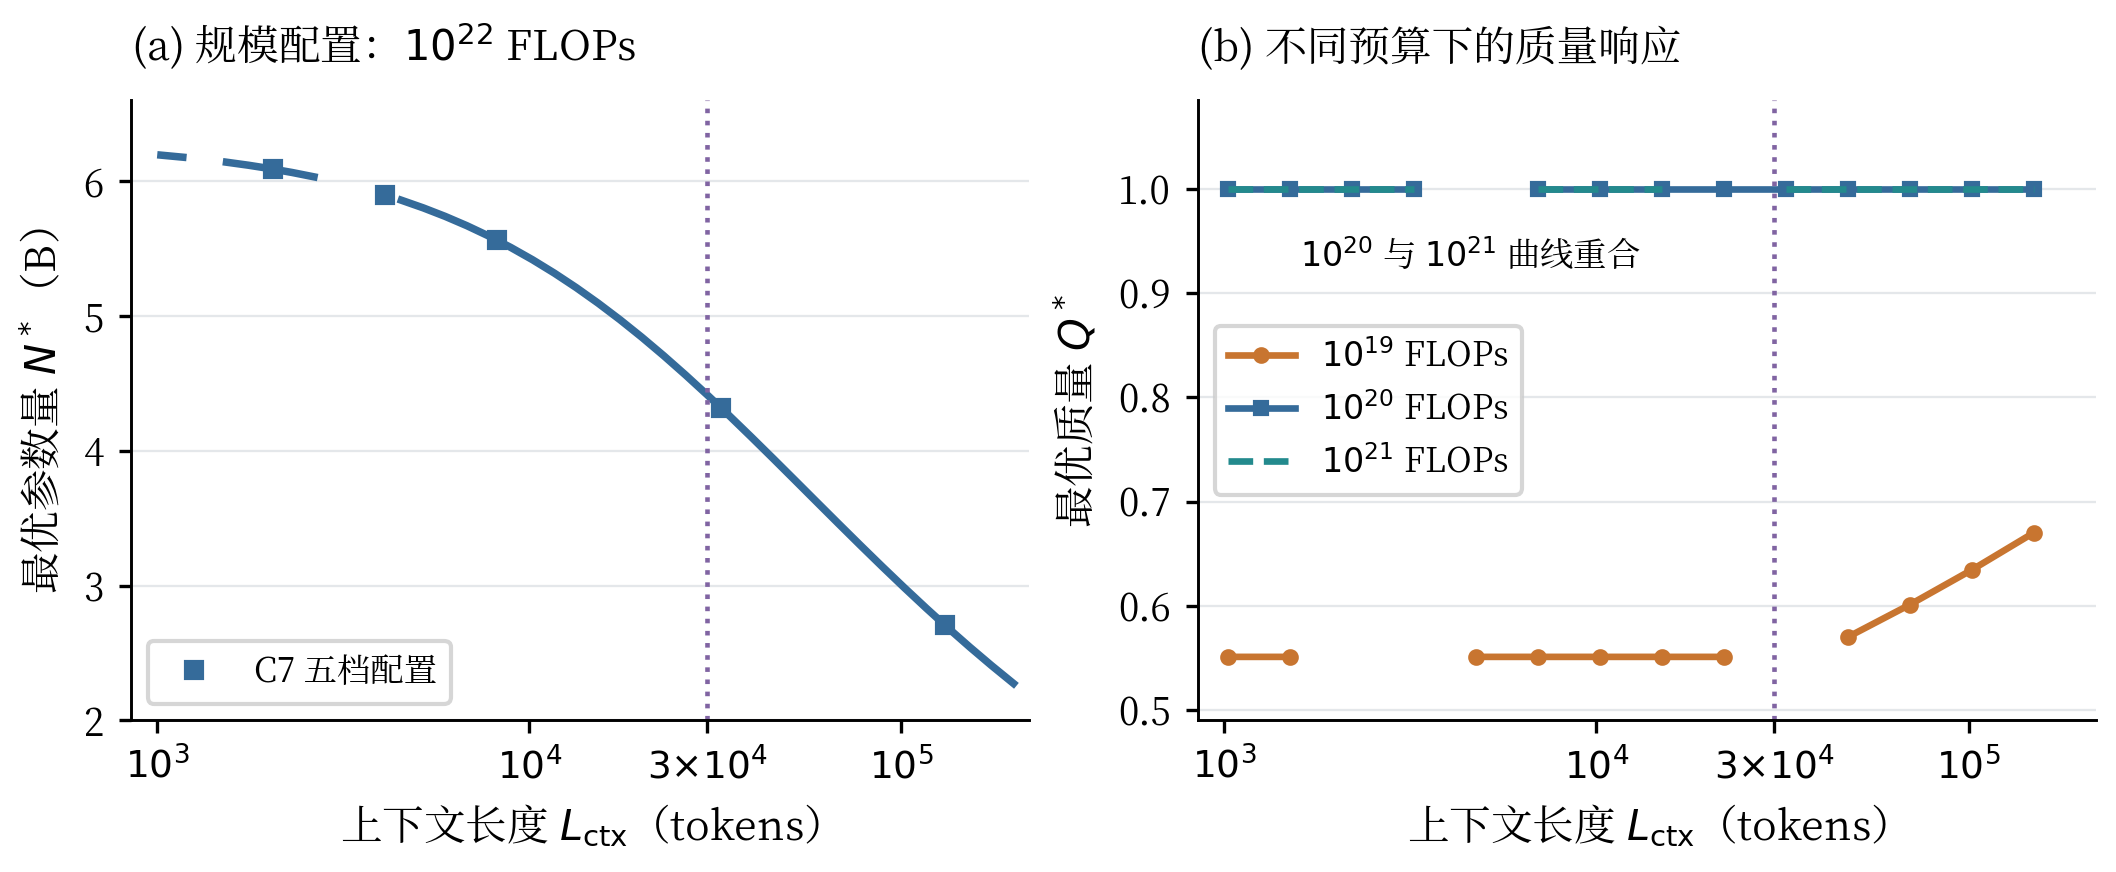
\includegraphics[width=0.94\textwidth]{../求解/问题三/图片/图3_上下文长度敏感性.png}
 \caption{上下文敏感性}
 \label{fig:p3_ctx}
\end{figure}

低预算的质量变化则不同。图\ref{fig:p3_ctx}右图中，$10^{19}$ FLOPs 的质量由 0.549 上升到约 0.671。按题设，质量处理总费用与数据量 $D$ 成正比；上下文延长后，可负担的数据变少，处理整份语料所需的费用也改变了，因此质量与规模之间的取舍随之变化。这一解释依赖当前的数据量成本关系。

\FloatBarrier

\textbf{4.固定配比平移的条件算例与适用范围}\par\nopagebreak[4]
领域配比会影响预训练效果\cite{xie2023doremi}。按问题一核岭预测的 $M=-0.1730$，保持共同费用基线，在 $10^{22}$ FLOPs 下得到相同的 $N,D,Q$，损失从 2.1451 平移至 1.9721。参考配比达到后一损失的模型等效预算约为 $1.691\times10^{23}$ FLOPs，即 16.9 倍。该换算依赖绝对损失差跨尺度不变，不能解释为实际训练加速比。

表\ref{tab:q23_review_m_amplitude}将收益幅度依次保留 $0$、$25\%$、$50\%$、$75\%$ 和 $100\%$，在满分配置下独立反解预算。全部幅度对应的 16.90739 倍与正式计算一致；仅保留一半时降至 3.49 倍。可见，等效预算对迁移幅度较敏感，这些人为设定的比例也没有置信区间含义。

\begin{table}[htbp]
 \centering
 \caption{固定损失平移幅度的条件算例}
 \label{tab:q23_review_m_amplitude}
 \renewcommand{\arraystretch}{1.15}
 \begin{tabularx}{0.94\textwidth}{@{}>{\raggedright\arraybackslash}X*{5}{>{\centering\arraybackslash}p{0.105\textwidth}}@{}}
 \toprule
 假定收益保留比例 & 0 & $25\%$ & $50\%$ & $75\%$ & $100\%$ \\
 \midrule
 等效预算倍数 & 1.00 & 1.81 & 3.49 & 7.30 & 16.91 \\
 \bottomrule
 \end{tabularx}
\end{table}

固定配比项只平移目标函数，成本或上下文变化则会移动预算边界，两类情景因此产生不同作用。另将核岭候选自身质量 0.5182 仅作为费用基线，在 $10^{22}$ FLOPs 下得到约 6.104B 参数、228.5B tokens，变化较小但不再完全相同。闭合参考质量 0.548753 对应的对照则约为 6.09049B、229.44095B。两项均另列保存，正式配置继续使用外生 $Q_0$。

质量未到上界时，新增预算同时影响质量和规模；达到上界后，质量处理继续付费，预算份额随模型扩大而降低。低预算尤其依赖处理成本，上下文则通过训练单价改变可用的数据量。把这些数值用于实际训练，还需核对评分尺度和外推范围，并确认高预算所需语料能否取得。数据受限训练研究已指出，重复使用数据的收益会递减\cite{muennighoff2023scaling}。本文尚未加入供给与重复训练约束，高预算解因此作为理论情景使用。

各情景共同采用问题二的点估计参数，结果表刻画的是这些参数给定时的配置差异。参数估计误差尚未转换为配置区间，因而表中精确到小数位的规模不应被理解为同等精度的工程需求。本文能够支持的是在既定评分、损失与费用关系下比较投入方向；实际资源安排还需结合可用语料、模型架构及任务要求判断这些条件是否成立。
\FloatBarrier
\endgroup

\subsection{问题四：技术演进分析与能力前沿预测}
\begingroup
\setlength{\tabcolsep}{4pt}
\renewcommand{\arraystretch}{1.15}
\clubpenalty=10000
\widowpenalty=10000

\subsubsection{能力度量与数据组织}

前三问比较的是训练后的验证损失，本问转而考察实际评测能力。我们先检查损失较低的模型是否也有较高得分，再分析历史增长中有多少与参数扩张有关，最后估计未来前沿。已有研究讨论过规模增加时的能力涌现\cite{wei2022emergent}，也指出评分方式可能造成看似突然的变化\cite{schaeffer2023mirage}。因此，本文同时保留综合分数和单项任务结果：先统一样本，分层拟合损失与得分，再用规模、时间回归分解增量，以饱和曲线和结构情景预测，并结合任务表现与资源记录讨论限制。

\noindent\textbf{辅助分析说明：} 本问数据整理、绘图与数值核对使用 Codex 辅助，模型为 GPT-5.4（OpenAI，2026-03-05）及 GPT-6 系列（OpenAI，2026-09-03 系列首次发布）\cite{ai_codex54,ai_codex6}。

\textbf{1.综合得分、许可筛选与时间变量}\par\nopagebreak[4]
综合得分取 Open LLM Leaderboard v2 六个维度的等权均值\cite{openllm2025}，记为 $\bar B$，满分为 100。六项分别是 IFEval 指令遵循、BBH 综合推理、MATH Lvl 5 数学、GPQA 研究生级问答、MUSR 多步推理和 MMLU-PRO 专业知识。均分便于比较整体变化，单项分数则用于判断具体能力的不足，两者分别使用。

\Needspace{6\baselineskip}
较近时期的变化使用 C1，长期趋势另以 C3 作参照。时间均按评测记录定义：年度回归取 $t=\text{年份}-2019$，月度前沿使用月中点 \mbox{$t=\text{年份}-2019+(\text{月}-0.5)/12$}，C3 的年度记录放在年中。这样，年度变量用于比较规模与能力的关系，月度变量用于观察较短时间内的前沿变化。

表\ref{tab:p4_funnel}列出样本筛选过程。先保留字段完整的记录，再按许可白名单确定本文讨论的开放权重范围。白名单为 apache-2.0、mit、gpl-3.0、cc-by-4.0、mpl-2.0、bsd-3-clause、cc-by-sa-4.0、openrail，以及 llama2、llama3、llama3.1、llama3.2、llama3.3、gemma。其他和未知许可不进入主样本；列入白名单只表示符合本研究的筛选规则，不代表各许可的使用条件相同。

\begin{table}[!htbp]
\centering
\caption{主样本的形成及模型类型构成}
\label{tab:p4_funnel}
\begin{tabularx}{0.98\textwidth}{@{}
>{\hsize=1\hsize\linewidth=\hsize\raggedright\arraybackslash}X
>{\hsize=0.45\hsize\linewidth=\hsize\centering\arraybackslash}X
>{\hsize=1.55\hsize\linewidth=\hsize\raggedright\arraybackslash}X@{}}
\toprule
数据层次 & 记录数 & 判定依据或构成 \\
\midrule
C1 原始记录 & 4{,}576 & 六维得分均完整；日期覆盖 2024-06 至 2025-03 \\
完整性筛选后 & 4{,}561 & 日期、参数量和六维得分齐备，排除 15 条记录 \\
许可白名单主样本 & 2{,}346 & 以 Hub License 字段匹配许可集合 \\
\midrule
预训练类 & 231 & pretrained 与持续预训练模型 \\
对话及微调类 & 1{,}497 & chat 与领域微调模型 \\
其他类型 & 618 & 包含 611 条合并模型记录和 7 条多模态记录 \\
\bottomrule
\end{tabularx}
\end{table}

表中的三类模型均保留在主样本中，类型只用于分组比较。为观察基础训练与后训练的差异，再分别估计预训练类、对话及微调类的规模和时间系数。C3 的历史记录则按六维得分一致性和参数有效性筛选，没有沿用 C1 的许可白名单，所以长期分析不能看成对同一批开放权重模型的持续追踪。

\textbf{2.从原始评测记录到子任务样本}\par\nopagebreak[4]
细分任务来自 C8，其 1{,}863 个模型目录共含 1{,}958 个 JSON 文件。每个目录优先读取最新文件，解析失败时再回退，最终 1{,}860 个目录取得有效结果，3 个没有可用记录。指标按 acc\_norm、acc、prompt\_level\_loose\_acc、inst\_level\_loose\_acc、exact\_match 的顺序选取，并换算为百分制。规范化模型名称后，与主样本对应的有 964 个目录。由此汇总 BBH 24 项、MATH-Hard 7 项、GPQA 3 项、MUSR 3 项，共 37 项任务，各项有效样本为 961 至 964 个。

C8 与 C1 的分数不能直接混用。前者保留原始指标，后者对汇总得分作了基准调整：GPQA 的随机基线为 0.25，MMLU-PRO 为 0.10，因此原始比例 $s$ 分别变为 $(s-0.25)/0.75$、$(s-0.10)/0.90$。IFEval 还对严格判定下的提示级、指令级结果取平均。本文因此用 C1 比较综合能力，用 C8 比较任务内部的原始表现。

按名称关联后，两套得分的比较见表\ref{tab:p4_c8chk}。C1 中同名的多条记录均保留，因此配对数可能多于 C8 目录数，不能当作独立模型数。六维 Spearman 系数均高于 0.81，多数高于 0.97，说明排序大体相近；但 BBH、GPQA、MUSR 的绝对差较大。排序接近并没有消除任务构成和归一化方式的差别。

\begin{table}[!htbp]
\centering
\caption{原始指标与汇总得分的记录级一致性}
\label{tab:p4_c8chk}
\begin{tabularx}{0.98\textwidth}{@{}
>{\hsize=1.4\hsize\linewidth=\hsize\raggedright\arraybackslash}X
>{\hsize=0.95\hsize\linewidth=\hsize\centering\arraybackslash}X
>{\hsize=0.8\hsize\linewidth=\hsize\centering\arraybackslash}X
>{\hsize=0.8\hsize\linewidth=\hsize\centering\arraybackslash}X
>{\hsize=1.05\hsize\linewidth=\hsize\centering\arraybackslash}X@{}}
\toprule
评测维度 & \makecell{有效配对\\记录数} & \makecell{秩相关\\$\rho$} & \makecell{线性相关\\$r$} & \makecell{平均绝对\\偏差 / 分} \\
\midrule
IFEval & 1{,}896 & 0.987 & 0.987 & 2.88 \\
BBH & 1{,}898 & 0.997 & 0.998 & 21.06 \\
MATH Lvl 5 & 1{,}897 & 0.812 & 0.803 & 3.47 \\
GPQA & 1{,}894 & 0.992 & 0.987 & 23.38 \\
MUSR & 1{,}894 & 0.977 & 0.973 & 30.73 \\
MMLU-PRO & 1{,}896 & 0.998 & 0.998 & 7.56 \\
\bottomrule
\end{tabularx}
\end{table}

\subsubsection{损失与评测得分的分层联系}

要将前三问的损失结果用于解释能力变化，首先需要检验二者的对应关系。设验证损失为 $L$，采用便于比较方向和误差的线性映射：
\begin{equation}
    \bar B = a + b\,L
\end{equation}
采用最小二乘估计该关系。C6 的高可比记录主要来自同模型、同验证集的 Pythia，可与附件 B 对照；中可比记录来自不同模型族和技术报告，验证集并不统一。我们分别拟合这两层，再报告合并样本与 C5 的对照结果，使来源差异能够在结果中体现。

\begin{figure}[!htbp]
\centering
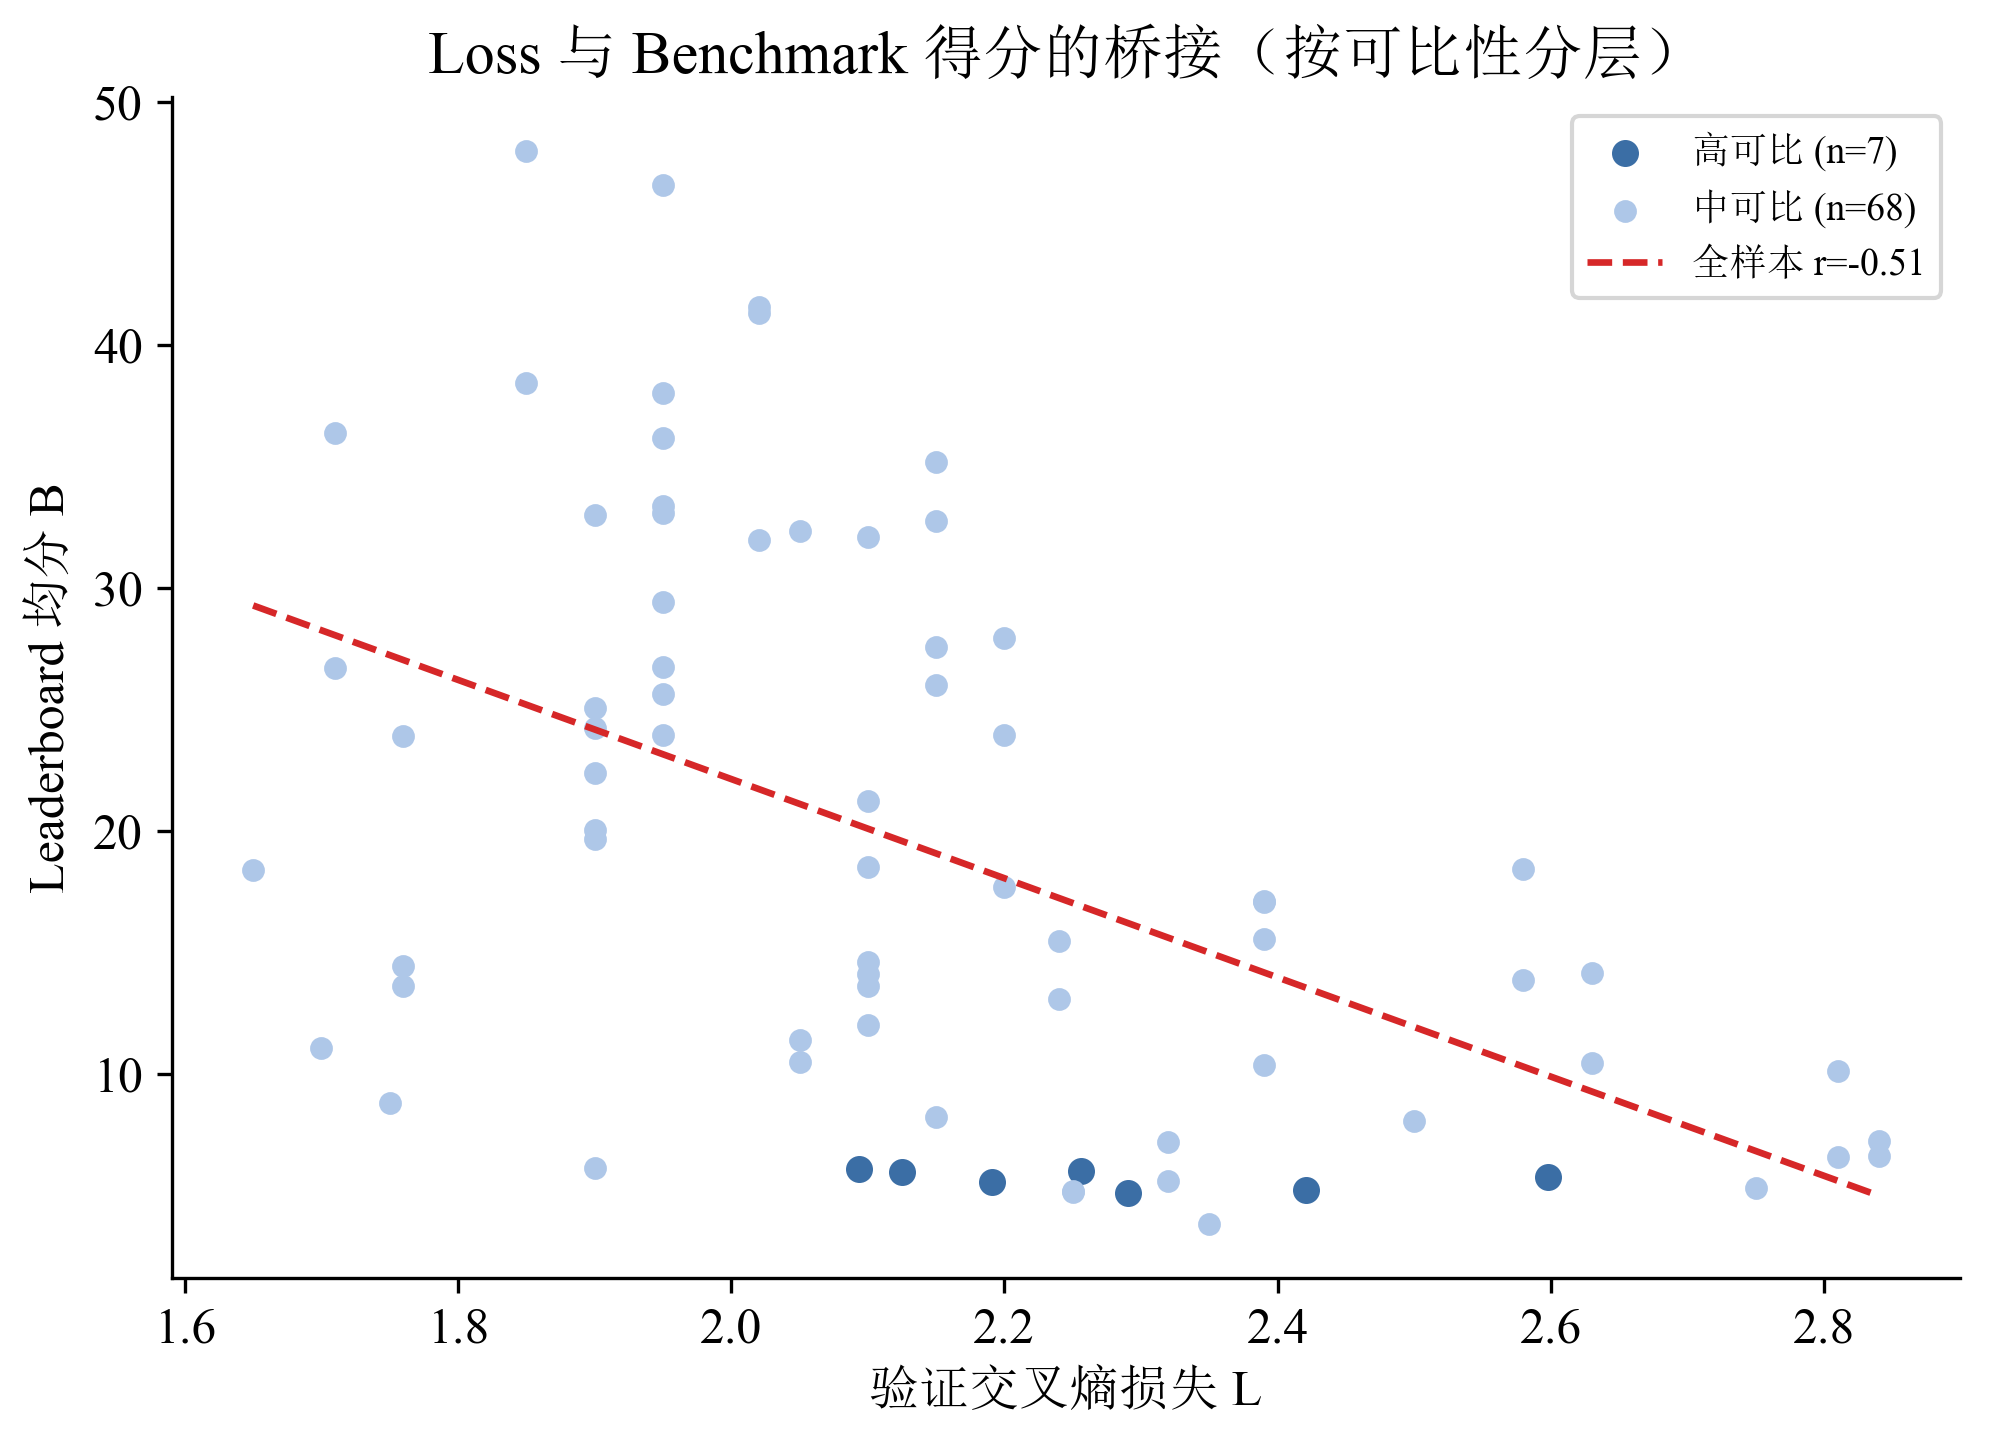
\includegraphics[width=0.98\textwidth]{../求解/问题四/图片/图1_Loss_Benchmark映射.png}
\caption{验证损失与得分的分层关系：点为 C6 记录，线为对应层的最小二乘拟合；两面板纵轴范围不同}
\label{fig:p4_map}
\end{figure}

\begin{table}[!htbp]
\centering
\caption{损失映射的方向、解释度与误差}
\label{tab:p4_bridge}
\begin{tabularx}{0.98\textwidth}{@{}
>{\hsize=1.25\hsize\linewidth=\hsize\raggedright\arraybackslash}X
>{\hsize=0.9375\hsize\linewidth=\hsize\centering\arraybackslash}X
>{\hsize=0.9375\hsize\linewidth=\hsize\centering\arraybackslash}X
>{\hsize=0.9375\hsize\linewidth=\hsize\centering\arraybackslash}X
>{\hsize=0.9375\hsize\linewidth=\hsize\centering\arraybackslash}X@{}}
\toprule
评价量 & \makecell{C6 高可比\\$n=7$} & \makecell{C6 中可比\\$n=68$} & \makecell{C6 合并\\$n=75$} & \makecell{C5 对照\\$n=43$} \\
\midrule
损失斜率 $b$ & $-0.882$ & $-19.185$ & $-20.417$ & $-16.155$ \\
Pearson $r$ & $-0.397$ & $-0.502$ & $-0.510$ & $-0.502$ \\
Spearman $\rho$ & $-0.607$ & $-0.509$ & $-0.549$ & — \\
决定系数 $R^2$ & 0.16 & 0.25 & 0.26 & — \\
MAPE / \% & 5.6 & 57.3 & 67.8 & — \\
\bottomrule
\end{tabularx}
\end{table}

图\ref{fig:p4_map}和表\ref{tab:p4_bridge}显示，损失较低时得分总体较高，但两者并没有形成精确的换算关系。合并样本的 Pearson $r=-0.510$、Spearman $\rho=-0.549$，$R^2$ 只有 0.26，MAPE 为 67.8\%。中可比层验证集不同，低得分又容易放大相对误差。高可比层虽有 5.6\% 的 MAPE，却只有 7 条记录，得分也仅在 $5.07\sim6.06$ 之间，不能据此推断高能力模型同样适用。

因此，这一步只支持损失与能力大体反向变化，不能把前三问的损失改善精确换成能力分，也不能由跨模型相关推断资源调整的因果效果。接下来的历史分解和预测直接使用 Benchmark 得分，以免继续传递这一换算误差。

\subsubsection{规模关系与历史增量分解}

\textbf{1.控制年份后的规模关联}\par\nopagebreak[4]
令 $P_{it}$ 表示模型参数量，单位为十亿参数。对模型记录建立包含规模和时间的回归，并以年份固定效应作对照：
\begin{equation}
    \text{Score}_{it} = b_0 + b_P\log_{10}P_{it} + b_t\,t + \varepsilon_{it}
    \qquad\text{或}\qquad
    \text{Score}_{it} = \alpha_t + b_P\log_{10}P_{it} + \varepsilon_{it}
\end{equation}
控制年份后，$b_P$ 表示参数量扩大十倍时的得分差；控制规模后，$b_t$ 表示每年的得分变化。$\alpha_t$ 用于表示各年的共同差异。上述系数描述条件关联，不能进一步分出数据工程、模型架构或对齐技术各自的因果作用。

主样本中，2024 年有 1{,}588 条，2025 年有 758 条。由于只有两个年份，线性年度变量与年份固定效应在这里可以表示同样的变化，得到相同的规模系数和 $R^2$ 并不意外，也不能当作两次独立验证。图\ref{fig:p4_scale}保留了每年内部的分散情况，表\ref{tab:p4_panel}进一步对照各类模型。

\begin{figure}[!htbp]
\centering
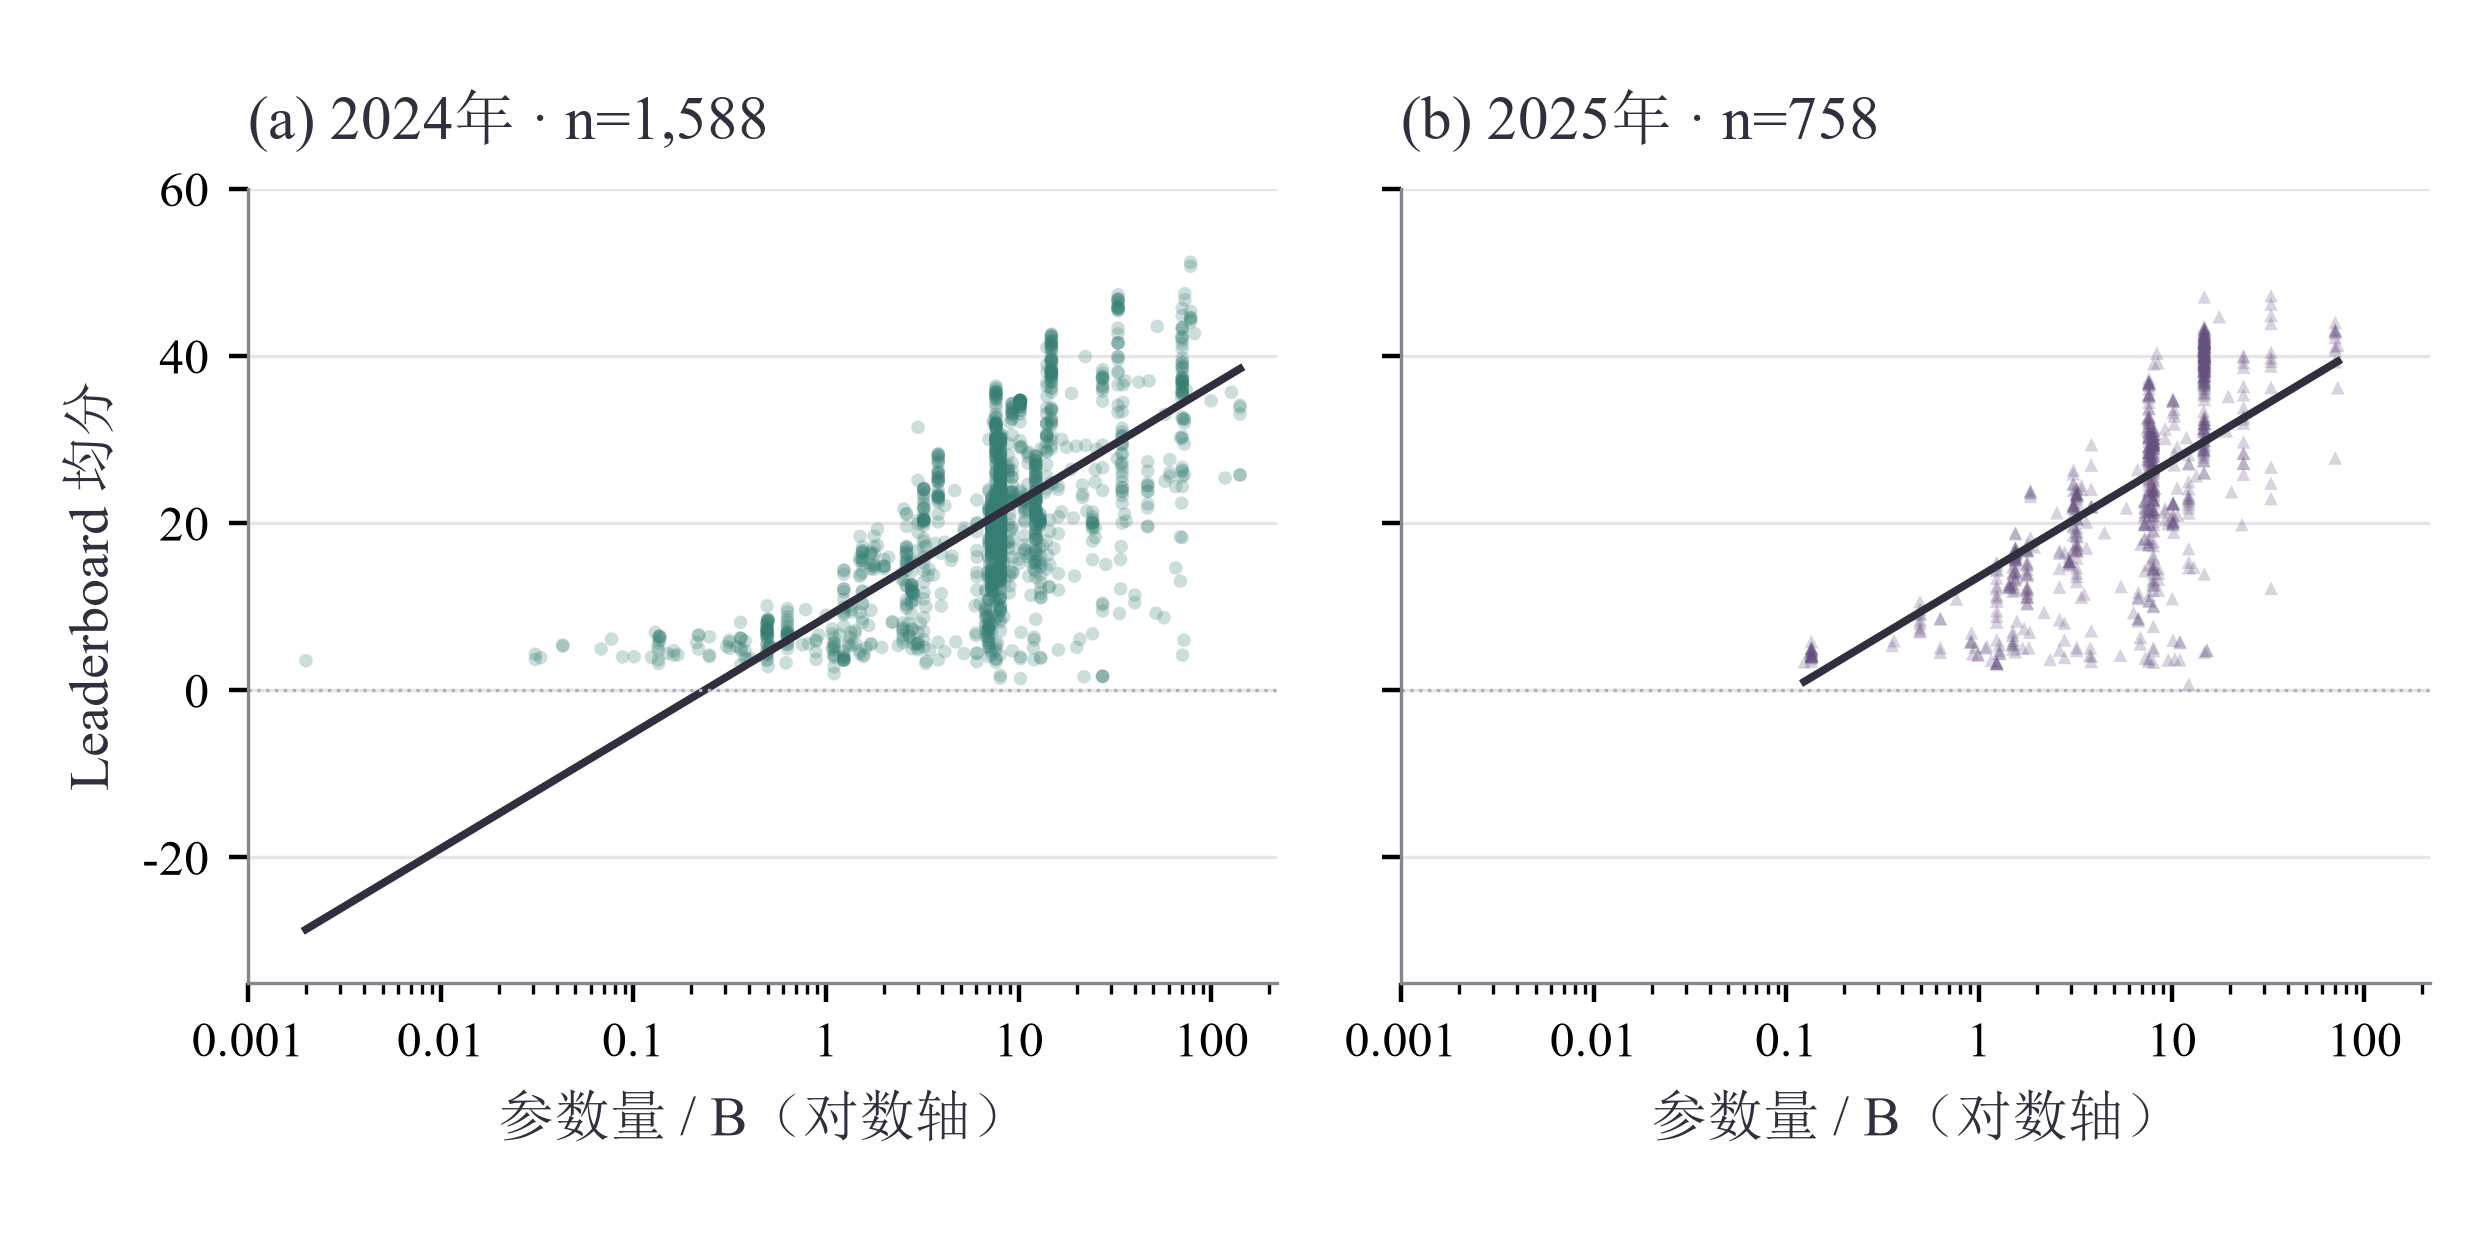
\includegraphics[width=0.98\textwidth]{../求解/问题四/图片/图7_年度规模效应.png}
\caption{按提交年份分组的规模与得分关系：点为主样本记录，直线使用同一规模系数及对应年份效应}
\label{fig:p4_scale}
\end{figure}

\begin{table}[!htbp]
\centering
\caption{全样本与类型子样本的规模、时间系数}
\label{tab:p4_panel}
\begin{tabularx}{0.98\textwidth}{@{}
>{\hsize=2\hsize\linewidth=\hsize\raggedright\arraybackslash}X
>{\hsize=0.6\hsize\linewidth=\hsize\centering\arraybackslash}X
>{\hsize=0.85\hsize\linewidth=\hsize\centering\arraybackslash}X
>{\hsize=0.85\hsize\linewidth=\hsize\centering\arraybackslash}X
>{\hsize=0.7\hsize\linewidth=\hsize\centering\arraybackslash}X@{}}
\toprule
样本与时间设定 & $n$ & \makecell{$b_P$\\分/十倍参数} & \makecell{$b_t$\\分/年} & $R^2$ \\
\midrule
主样本，年份固定效应 & 2{,}346 & 13.842 & — & 0.475 \\
主样本，线性年度项 & 2{,}346 & 13.842 & 4.844 & 0.475 \\
预训练类，线性年度项 & 231 & 6.414 & 1.552 & 0.460 \\
对话及微调类，线性年度项 & 1{,}497 & 14.853 & 4.680 & 0.484 \\
\bottomrule
\end{tabularx}
\end{table}

全样本的规模、年度系数分别为 13.842、4.844；预训练类为 6.414、1.552；对话及微调类为 14.853、4.680。不同类型的差异说明，解释回归时需要考虑样本构成。这里没有同一模型微调前后的受控比较，故不能直接认定微调提高了参数利用效率。此外，线性式在极小参数端可能预测负分，本节只用它概括规模关系和核算增量，不把它当作适用于全部规模的有界评分函数。

\textbf{2.长周期与近端窗口的贡献核算}\par\nopagebreak[4]
为量化历史增量，采用 shift-share 分解，将前沿得分变化拆为规模项与剩余项：
\begin{equation}
    \Delta F = \underbrace{b_P\,\Delta\log_{10}P_{\text{frontier}}}_{\text{规模扩张贡献}}
    + \underbrace{\left[\Delta F - b_P\,\Delta\log_{10}P_{\text{frontier}}\right]}_{\text{非规模技术进步贡献}}
\end{equation}
非规模项按总增量减去规模项计算，既可能包含技术改进，也会吸收样本更替、未观测因素和测量差异。将两项各自除以 $\Delta F$，便得到对应占比。

长期与近期采用不同的前沿定义。C3 以年度累计最高分表示 $F$，用当年保留记录的最大参数量代表规模，两者未必来自同一模型。C1 则取每月前 $1\%$ 得分均值，并使用该前列组中的最大参数量，比较首月到峰值月的变化。因此，两种占比分别对应不同时间尺度，不能合并求平均。

清理 C3 时发现 13 条记录的 Average 与六维均分相差超过 5 分，故将其排除。最大差约 42.3 分，来自 GPT-3 175B：Average 为 50.0，六维均分为 7.67。清理后，长期回归得到 $b_P=14.10$、$b_t=3.30$、$R^2=0.42$。2019 至 2025 年，累计前沿从 5.00 增至 52.08，总增量 47.08 分；规模项对应 23.77 分，非规模项为 23.31 分，占 50.5\% 和 49.5\%。由于历史评测来源仍有差异，这组结果主要用于比较长期量级。

\begin{figure}[!htbp]
\centering
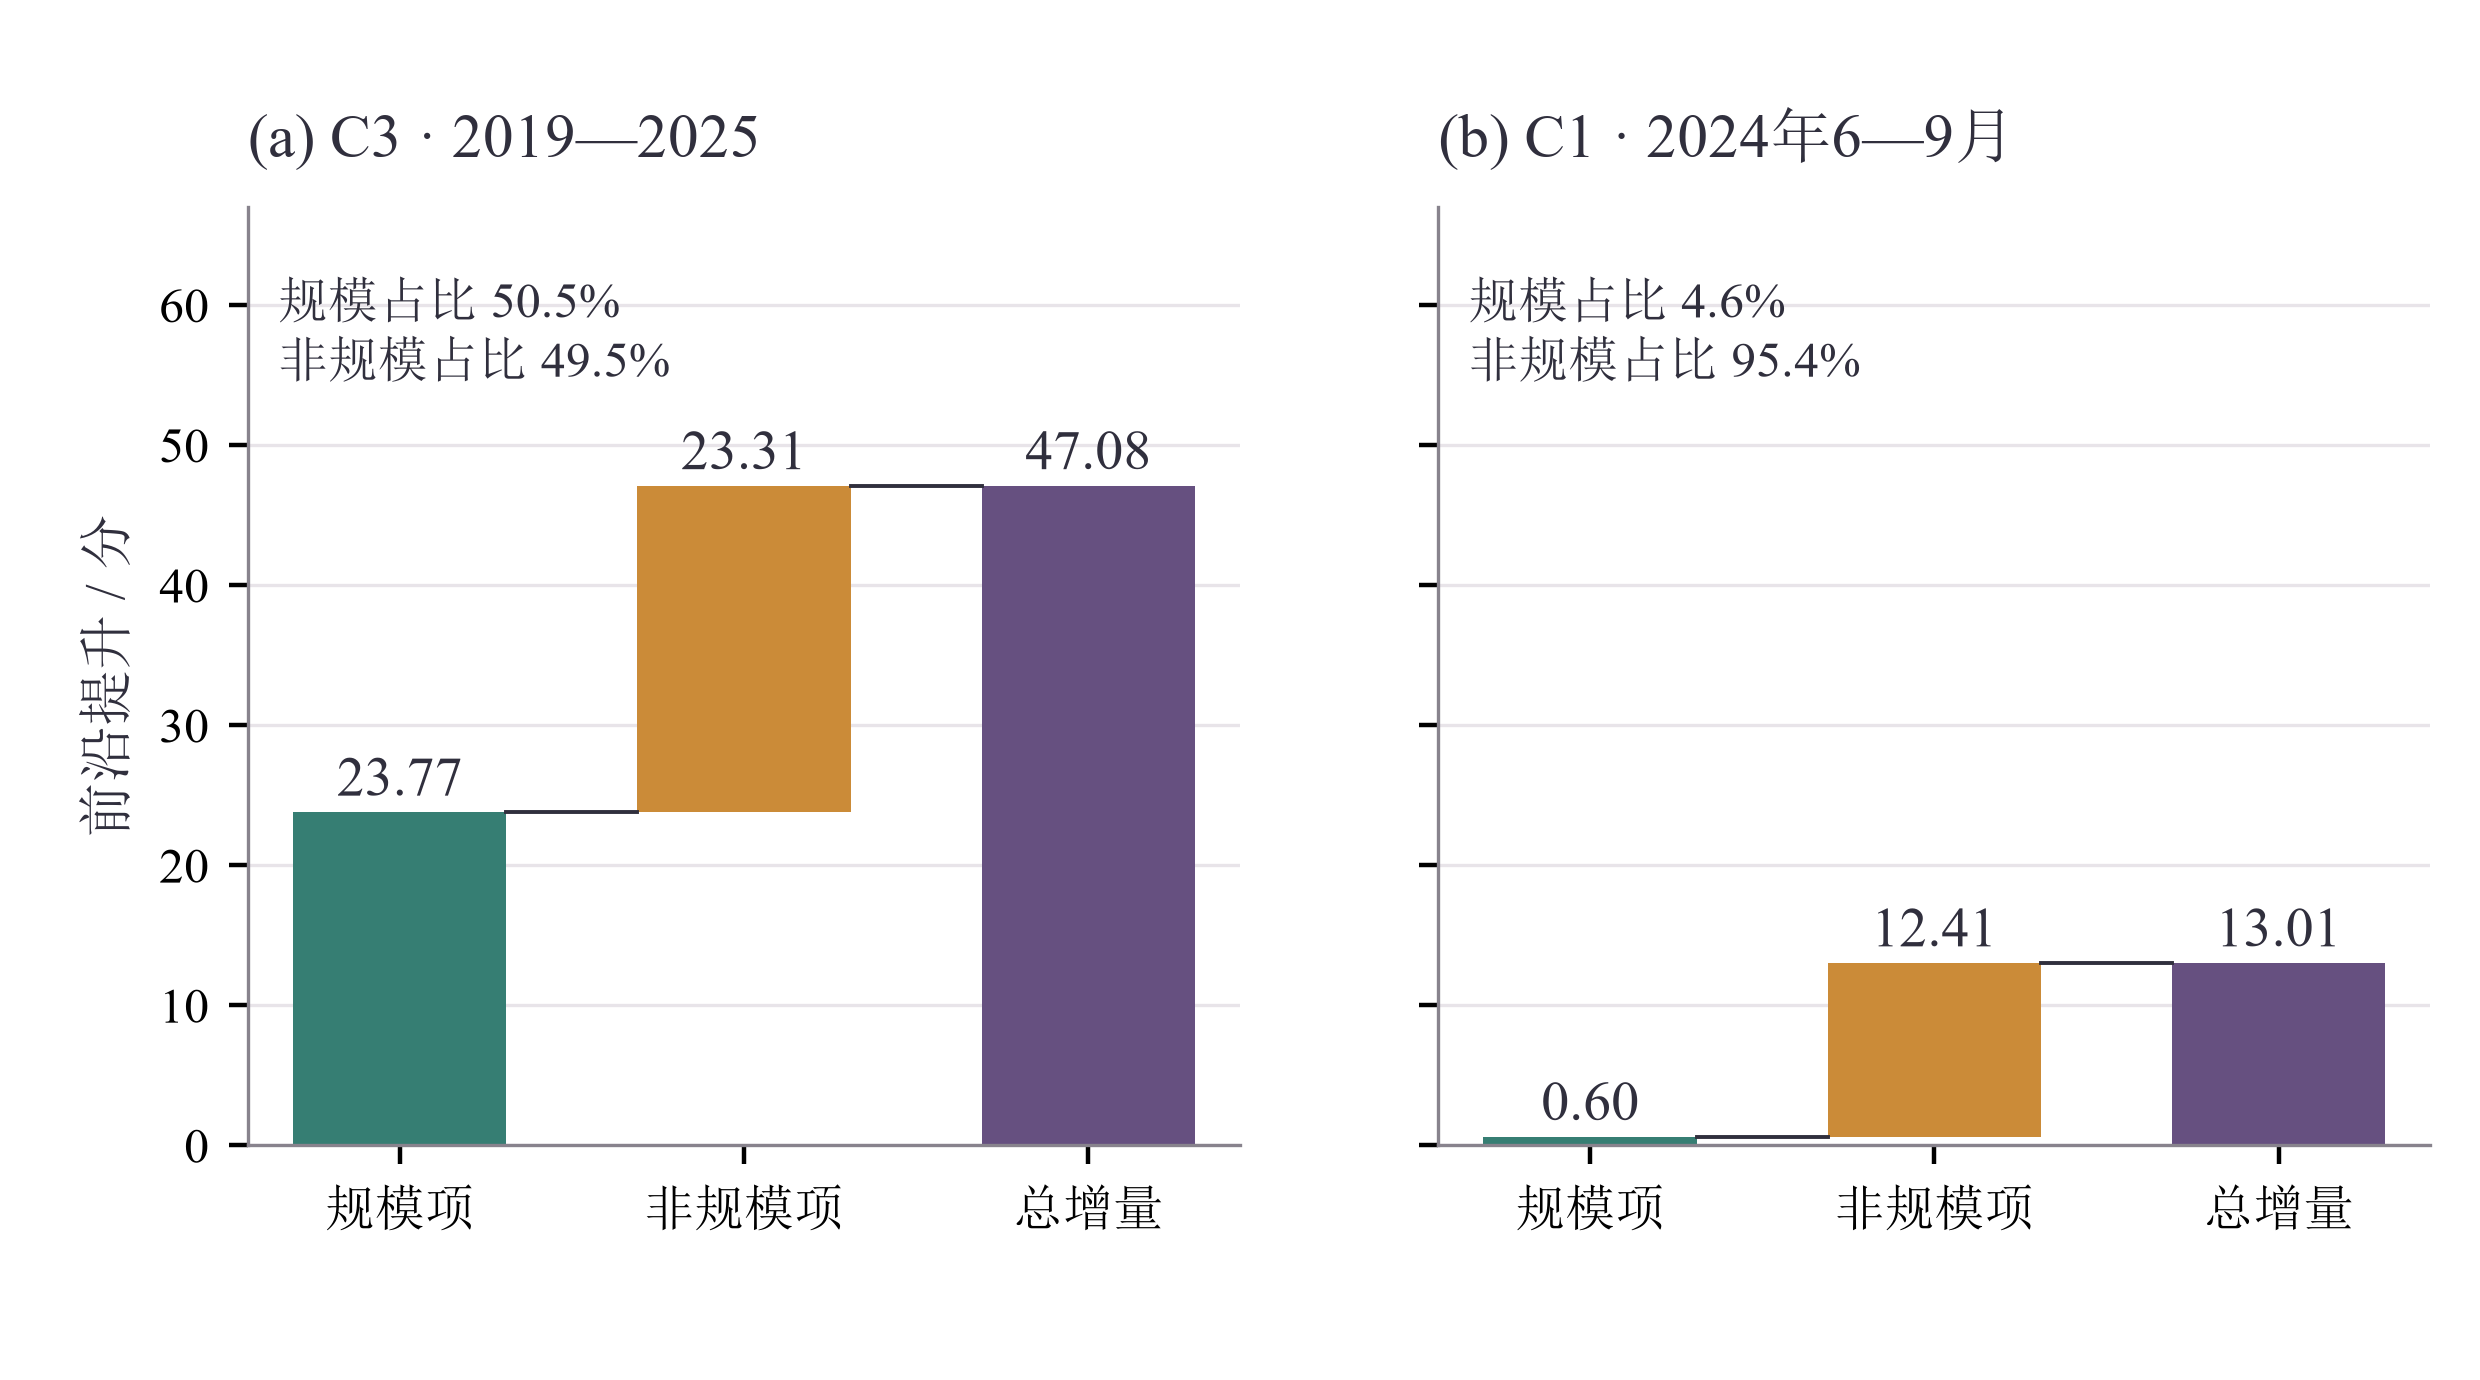
\includegraphics[width=0.98\textwidth]{../求解/问题四/图片/图2_规模时间分解.png}
\caption{两个时间窗口的前沿增量分解：规模项与非规模项相加为总增量；非规模项为分解后的剩余部分}
\label{fig:p4_decomp}
\end{figure}

\Needspace{6\baselineskip}
再看评测框架一致的 C1。2024 年 6 月至 9 月，前沿从 37.99 增至 51.00，而前列组最大参数量只由 70.6B 增至 78.0B，即 $\Delta\log_{10}P=0.043$。分解得到规模项 0.60 分、非规模项 12.41 分，占 4.6\%、95.4\%。图\ref{fig:p4_decomp}表明，这一短窗口的大部分增长不能由参数扩张解释；但其余部分不能直接归为某一种算法作用，也不能将该比例推广到整年或未来。

\subsubsection{前沿曲线与条件预测}

\textbf{1.饱和曲线及重抽样区间}\par\nopagebreak[4]
为预测前沿，将 C3 在 2019 至 2023 年的年度累计最高分，与 C1 月度前 $1\%$ 均值的累计最大值连接，共得到 14 个点。每月前列组人数按记录数的 $1\%$ 向下取整，最少取 1 个。采用 logistic 函数描述逐渐放缓的增长，并限制其上界不超过 100：
\begin{equation}
    F(t) = \frac{K}{1+e^{-r(t-t_0)}},\qquad K \text{ 为饱和上界},\ r \text{ 为增长率},\ t_0 \text{ 为拐点}
\end{equation}
估计结果为 $K=56.61$、$r=2.523$、$t_0=5.11$，拟合 $R^2=0.975$。随后对残差作 600 次 bootstrap 重抽样，用成功重拟合预测值的第 5、第 95 百分位组成 $90\%$ 区间。这反映的是既定曲线下的抽样波动，尚未覆盖评测标准和未来技术路径改变带来的全部不确定性。

算力增长放缓情景以“增速减半”实现：
\begin{equation}
    F_{\text{slow}}(t)=K\left[1+e^{-r(\min(t,t_h)-t_0)}\right]^{-1},\qquad t_h \text{ 为增速减半时刻}
\end{equation}

\textbf{2.基于规模和年度系数的结构情景}\par\nopagebreak[4]
为考察不预设短期饱和时的变化，利用规模和年度系数作结构外推：
\begin{equation}
    \hat F(t+\Delta) = F(t) + \left[b_P\,\Delta\log_{10}P + b_t\right]\cdot\Delta
\end{equation}
式中，$\Delta$ 为向前预测的年数，$\Delta\log_{10}P$ 为假设的\emph{年均}参数对数增量。设置三种条件进行比较：基准情景保持规模不变并延续 $b_t$；放缓情景同样固定规模，但把 $b_t$ 减半；扩容情景则令规模每年增加 0.3 个数量级，同时保留 $b_t$。其中放缓幅度是对非规模增长的假设，并不是从算力增速估计出的传导关系。

\begin{figure}[!htbp]
\centering
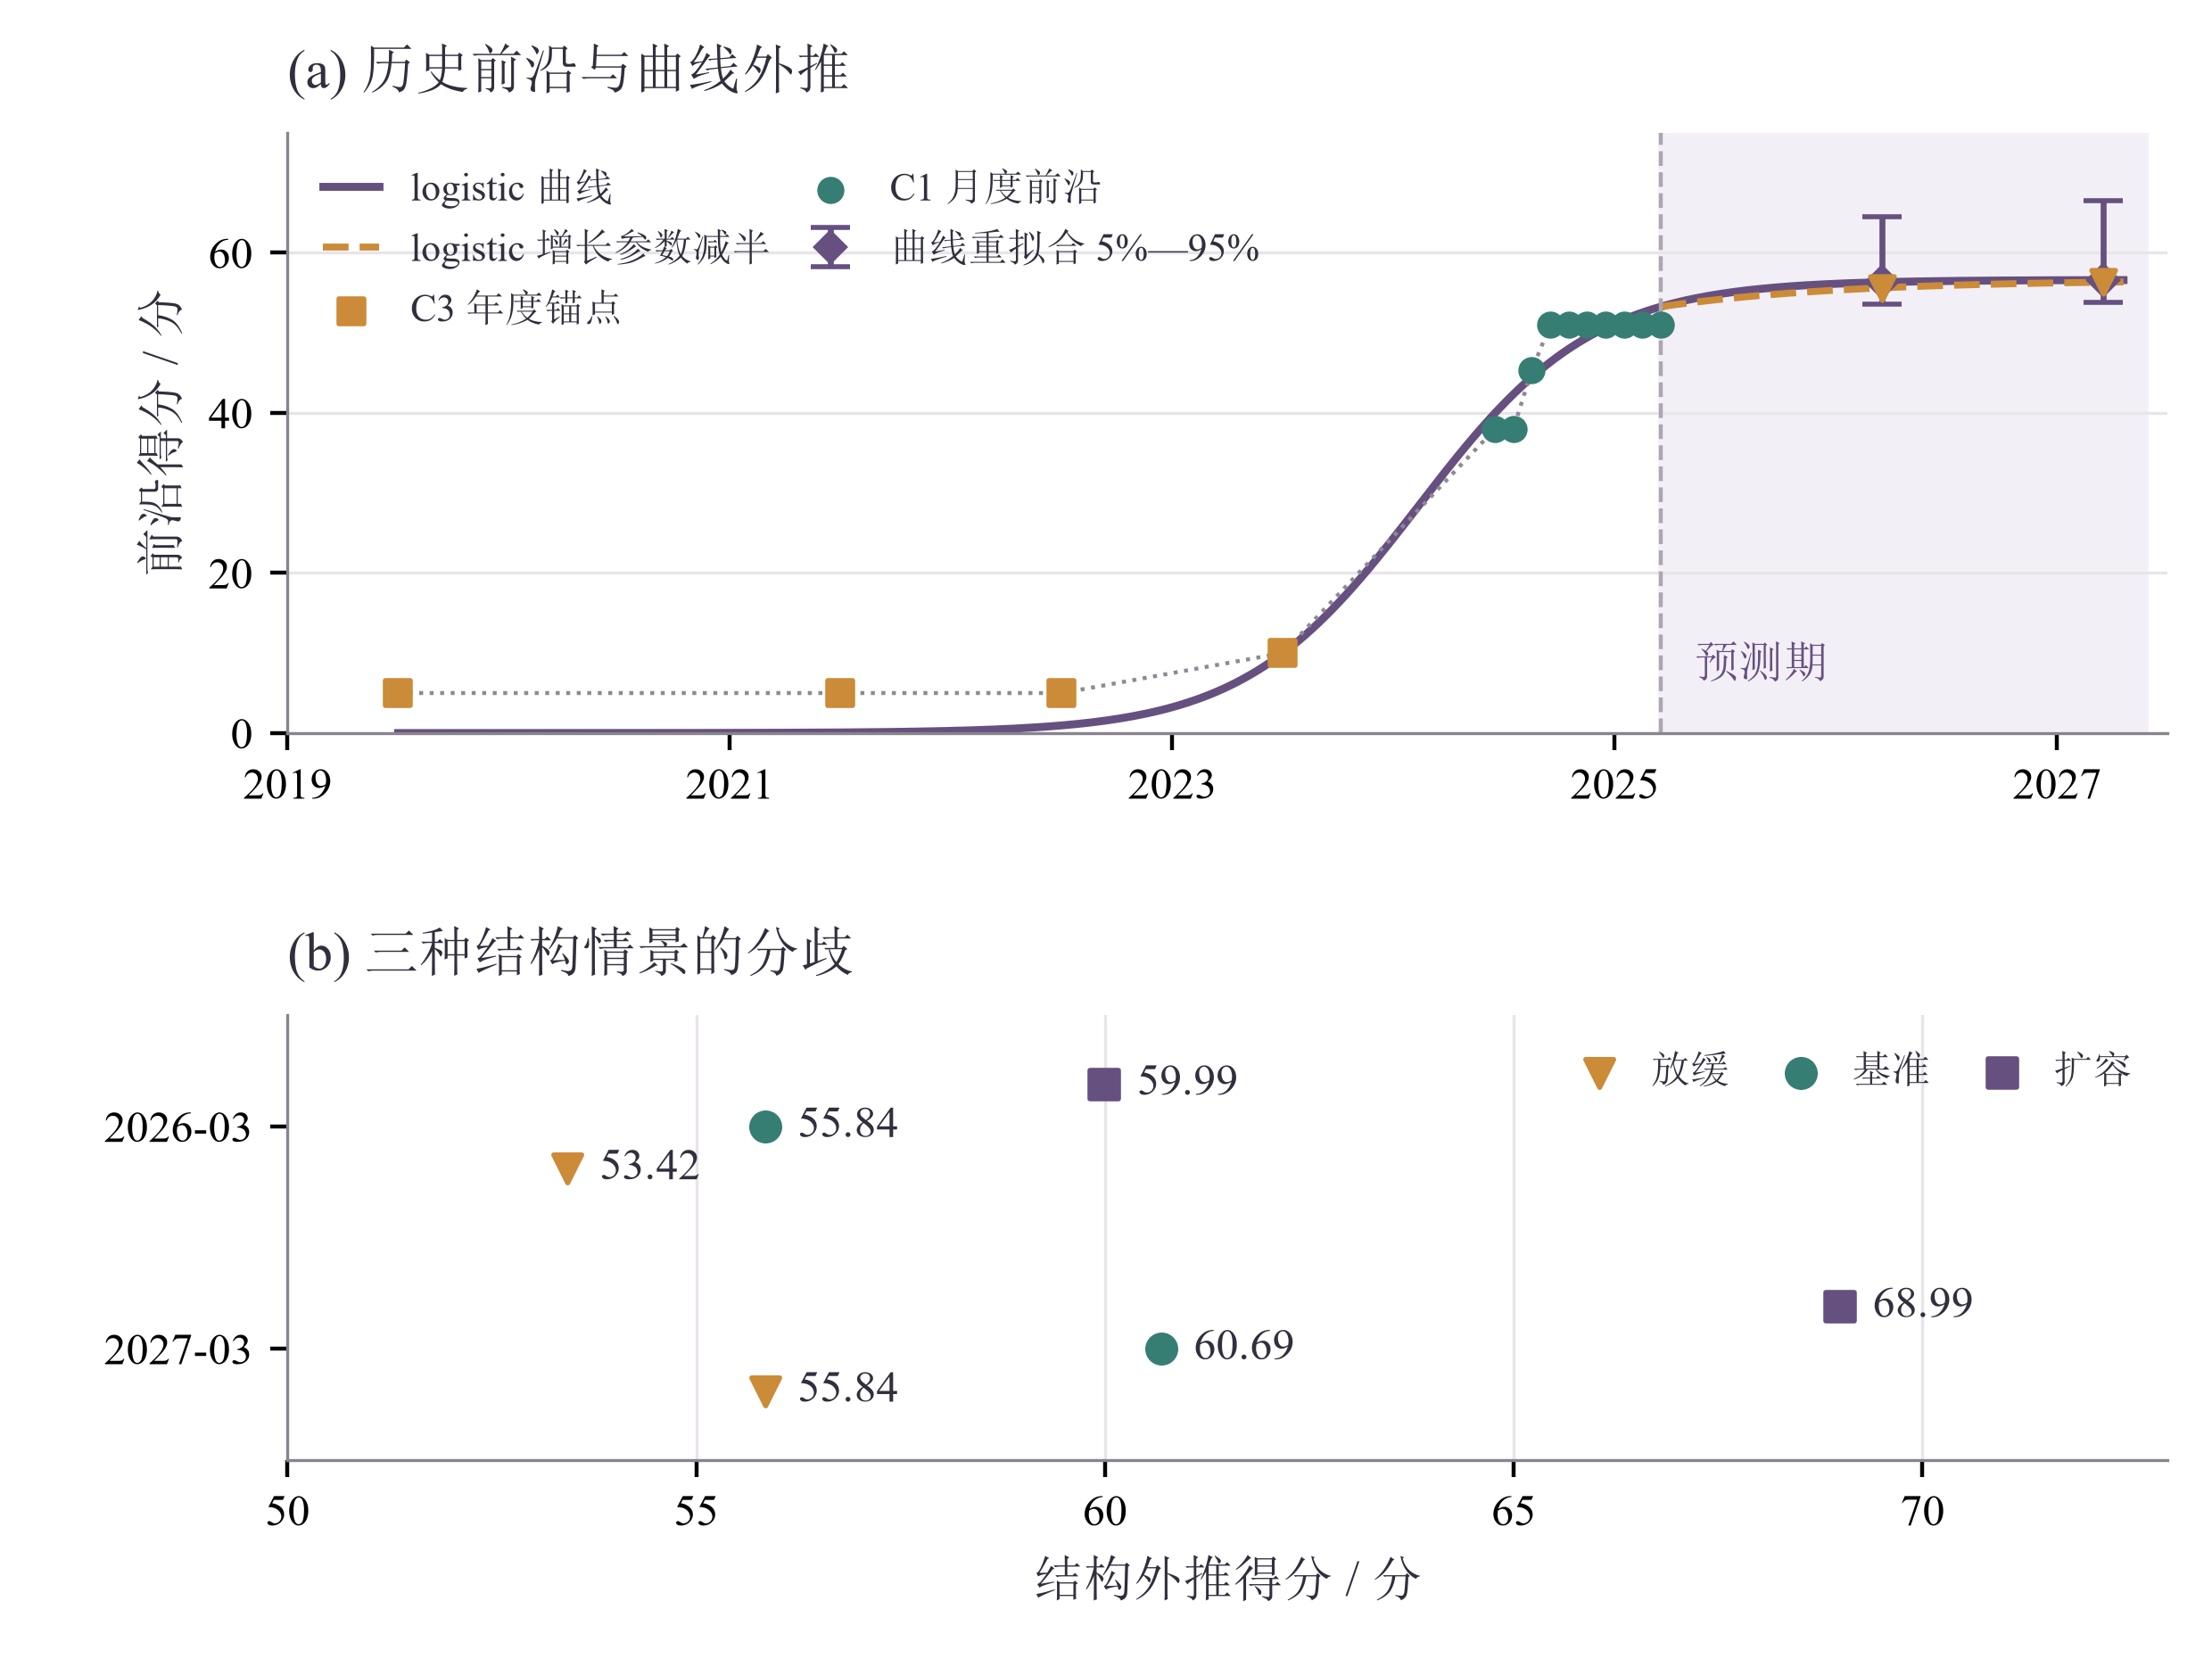
\includegraphics[width=0.98\textwidth]{../求解/问题四/图片/图3_能力前沿预测.png}
\caption{历史前沿与条件预测：上图误差棒为两个预测时点的 $90\%$ bootstrap 区间，下图为结构情景点值}
\label{fig:p4_frontier}
\end{figure}

\begin{table}[!htbp]
\centering
\caption{以 2025 年 3 月数据为基点的能力前沿预测}
\label{tab:p4_frontier}
\begin{tabularx}{0.98\textwidth}{@{}>{\raggedright\arraybackslash}X >{\centering\arraybackslash}X >{\centering\arraybackslash}X@{}}
\toprule
预测口径 & \makecell{前瞻 12 个月\\2026-03} & \makecell{前瞻 24 个月\\2027-03} \\
\midrule
logistic 点预测 & 56.33 & 56.59 \\
bootstrap 第 5 百分位 & 53.62 & 53.75 \\
bootstrap 第 95 百分位 & 64.52 & 66.52 \\
logistic 增速减半 & 53.27 & 53.27 \\
\midrule
结构外推：规模持平 & 55.84 & 60.69 \\
结构外推：非规模增速减半 & 53.42 & 55.84 \\
结构外推：每年扩容 0.3 dex & 59.99 & 68.99 \\
\bottomrule
\end{tabularx}
\end{table}

预测从附件的观测截止时点出发，基点位于 2025 年 3 月，12、24 个月后分别为 2026 年 3 月和 2027 年 3 月。表\ref{tab:p4_frontier}中，logistic 基准预测约为 56.3、56.6 分，$90\%$ 区间为 $[53.62,64.52]$、$[53.75,66.52]$。结构模型的三种情景分别落在 $53.42\sim59.99$ 和 $55.84\sim68.99$ 分，向外取整可概括为 $53\sim60$、$55\sim69$ 分。这一范围来自不同情景的点预测，含义不同于置信区间。

两种预测的主要差别见图\ref{fig:p4_frontier}：饱和曲线在两期之间几乎不再上升，结构基准则假设年度增量继续存在。结构放缓情景得到 53.42、55.84 分，仍有增长，只是速度降低。C1 可比观测约为 10 个月，而前瞻已是其 $1.2\sim2.4$ 倍，早期 C3 又存在评分差异。因此，高拟合度不能代替未来检验，上述数值应与评分体系和情景假设一同使用。

\subsubsection{从综合前沿到具体任务瓶颈}

\textbf{1.六维能力的分布差异}\par\nopagebreak[4]
综合分数还不能说明各项能力是否同时提高。图\ref{fig:p4_distribution}展开六维分布，表\ref{tab:p4_task}列出中位数、前列均值和最高分，使整体水平与领先水平能够同时比较。距满分差值按 $100-\text{最优得分}$ 计算，只表示当前评分上的差距，不能当作一定可以实现的提升量。

\begin{figure}[!htbp]
\centering
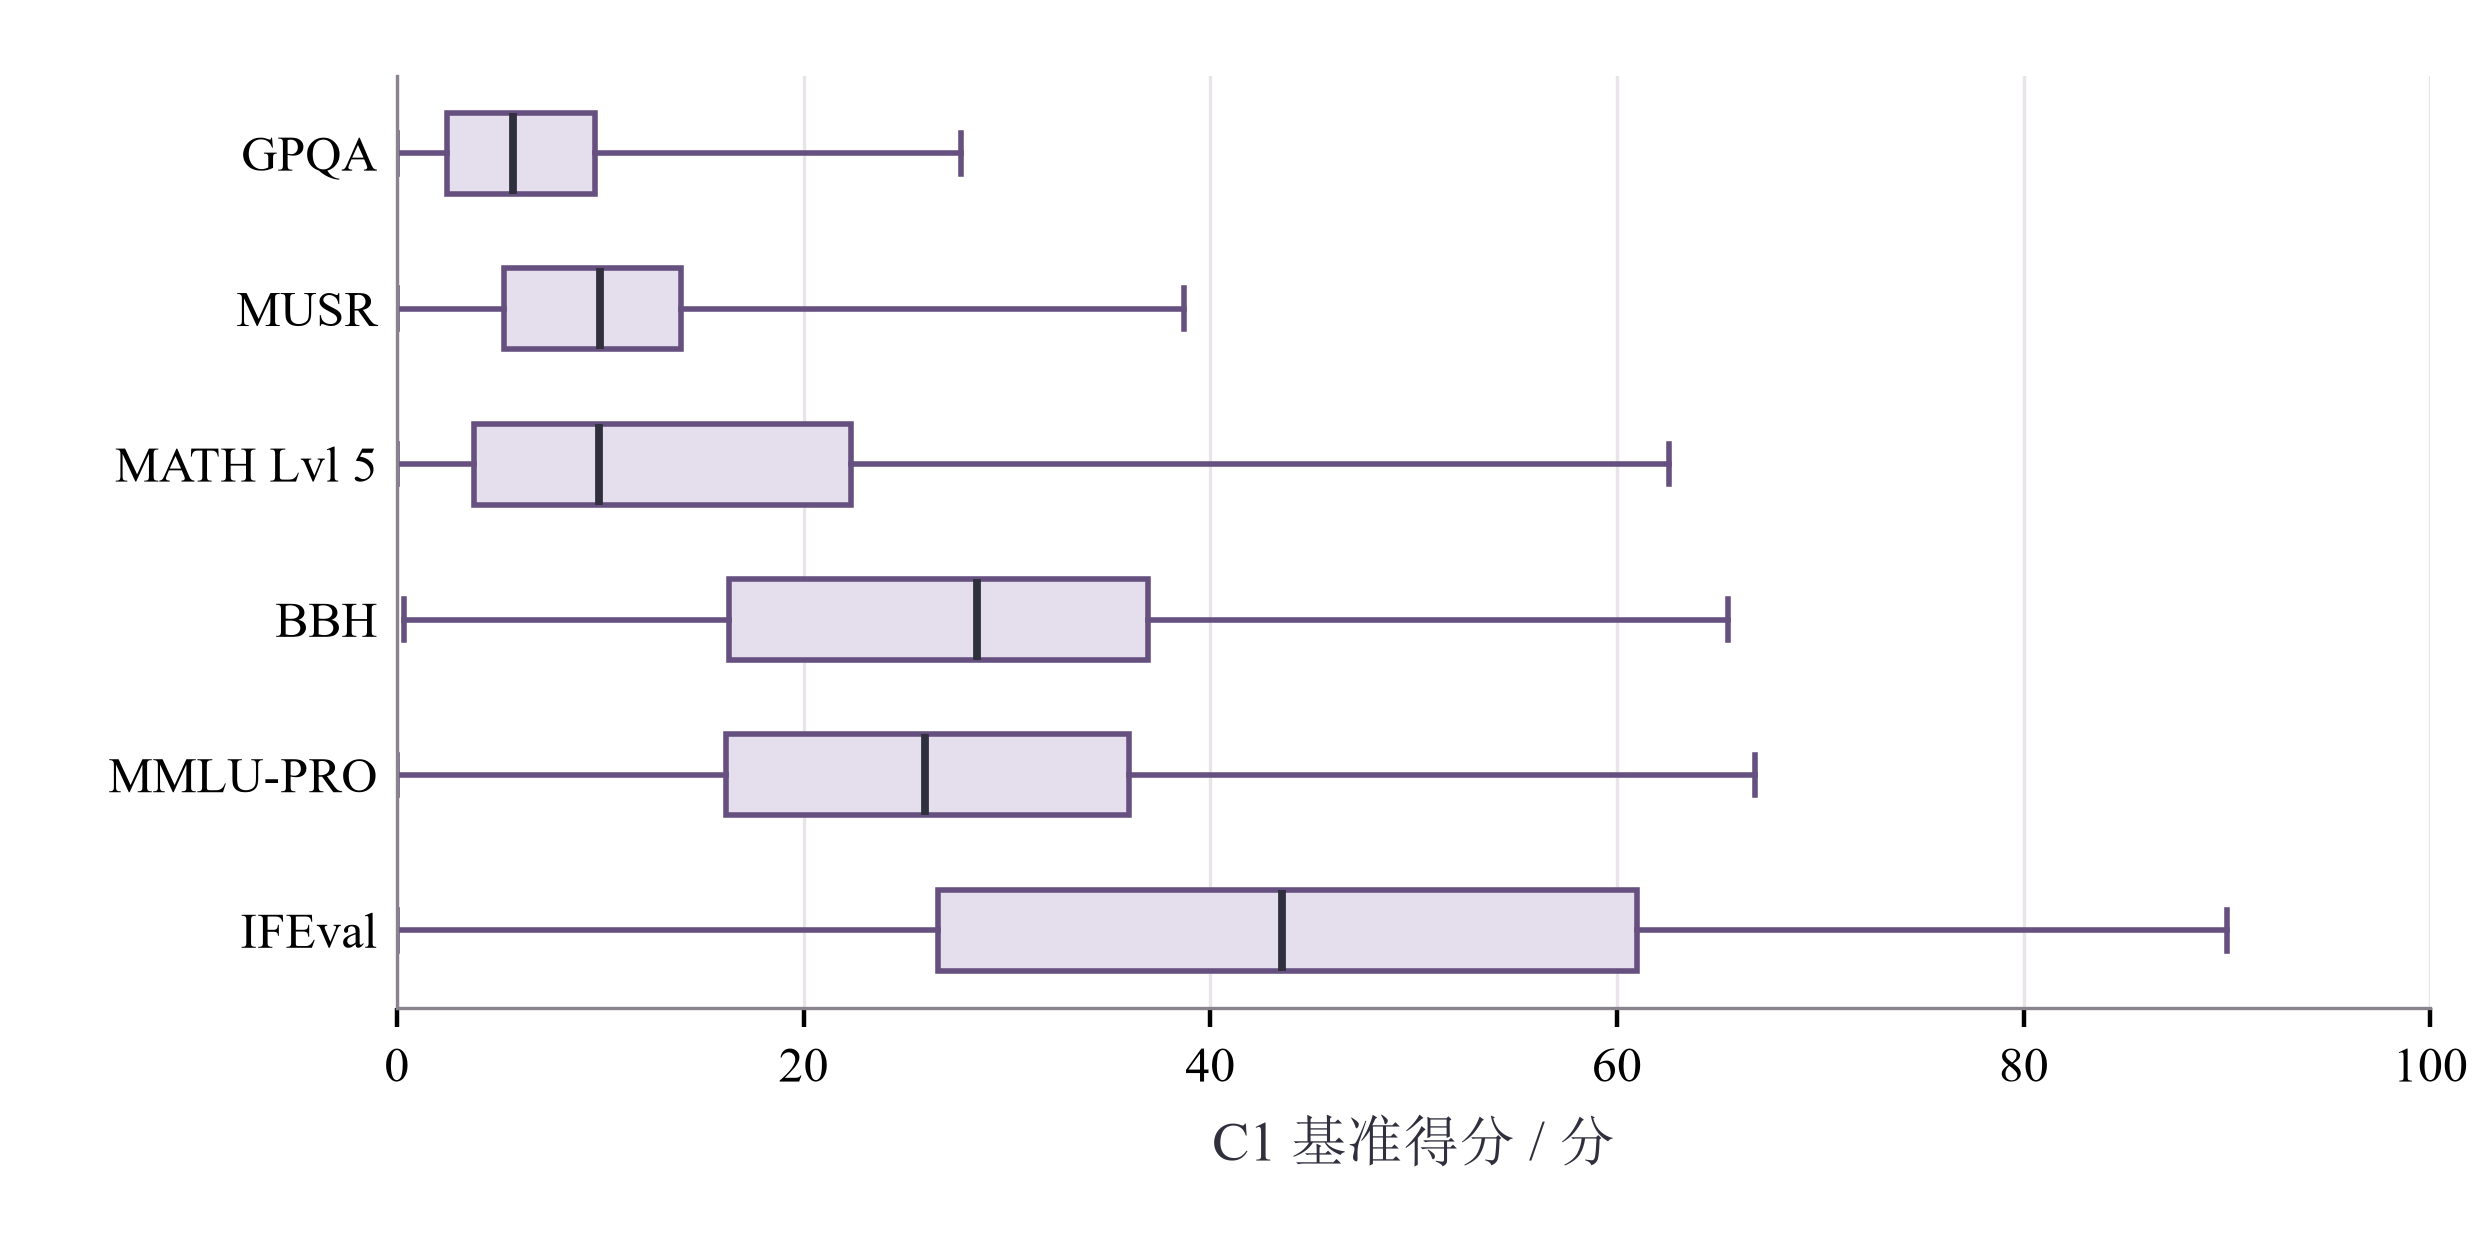
\includegraphics[width=0.98\textwidth]{../求解/问题四/图片/图6_六维能力分布.png}
\caption{主样本的六维能力分布：每维 $n=2{,}346$，箱体为第 25 至第 75 百分位，箱内线为中位数，须线为最小值至最大值}
\label{fig:p4_distribution}
\end{figure}

\begin{table}[!htbp]
\centering
\caption{六维能力的总体水平与前沿差距}
\label{tab:p4_task}
\begin{tabularx}{0.98\textwidth}{@{}
>{\hsize=1.3\hsize\linewidth=\hsize\raggedright\arraybackslash}X
>{\hsize=0.85\hsize\linewidth=\hsize\centering\arraybackslash}X
>{\hsize=1.05\hsize\linewidth=\hsize\centering\arraybackslash}X
>{\hsize=0.9\hsize\linewidth=\hsize\centering\arraybackslash}X
>{\hsize=0.9\hsize\linewidth=\hsize\centering\arraybackslash}X@{}}
\toprule
任务维度 & 中位数 & 前 $1\%$ 均值 & 最优得分 & \makecell{距满分差值\\/ 分} \\
\midrule
GPQA & 5.70 & 22.80 & 27.74 & 72.3 \\
MUSR & 9.97 & 28.06 & 38.69 & 61.3 \\
MATH Lvl 5 & 9.93 & 58.02 & 62.54 & 37.5 \\
BBH & 28.52 & 59.95 & 65.47 & 34.5 \\
MMLU-PRO & 25.98 & 55.26 & 66.80 & 33.2 \\
IFEval & 43.51 & 84.45 & 89.98 & 10.0 \\
\bottomrule
\end{tabularx}
\end{table}

IFEval 最高为 89.98，离满分仅 10.0 分，但中位数仍为 43.51，因此只能说少数领先模型得分较高，不能说整个样本接近饱和。GPQA、MUSR 最高分别为 27.74、38.69，中位数更低，是比较明显的薄弱项。数学的情况也有分化：MATH Lvl 5 最高为 62.54，中位数只有 9.93，说明前沿改善尚未普遍体现在大多数模型上。

\textbf{2.原始子任务中的瓶颈位置}\par\nopagebreak[4]
再把 C8 的 37 个子任务按类别展开，见图\ref{fig:p4_task}。每项同时画出中位数、前 $5\%$ 均值和最高分，分别观察普通样本、前列组和单项前沿。表\ref{tab:p4_sub}列出距满分差值最大的六项，中文名称与图中对应。

\begin{figure}[!htbp]
\centering
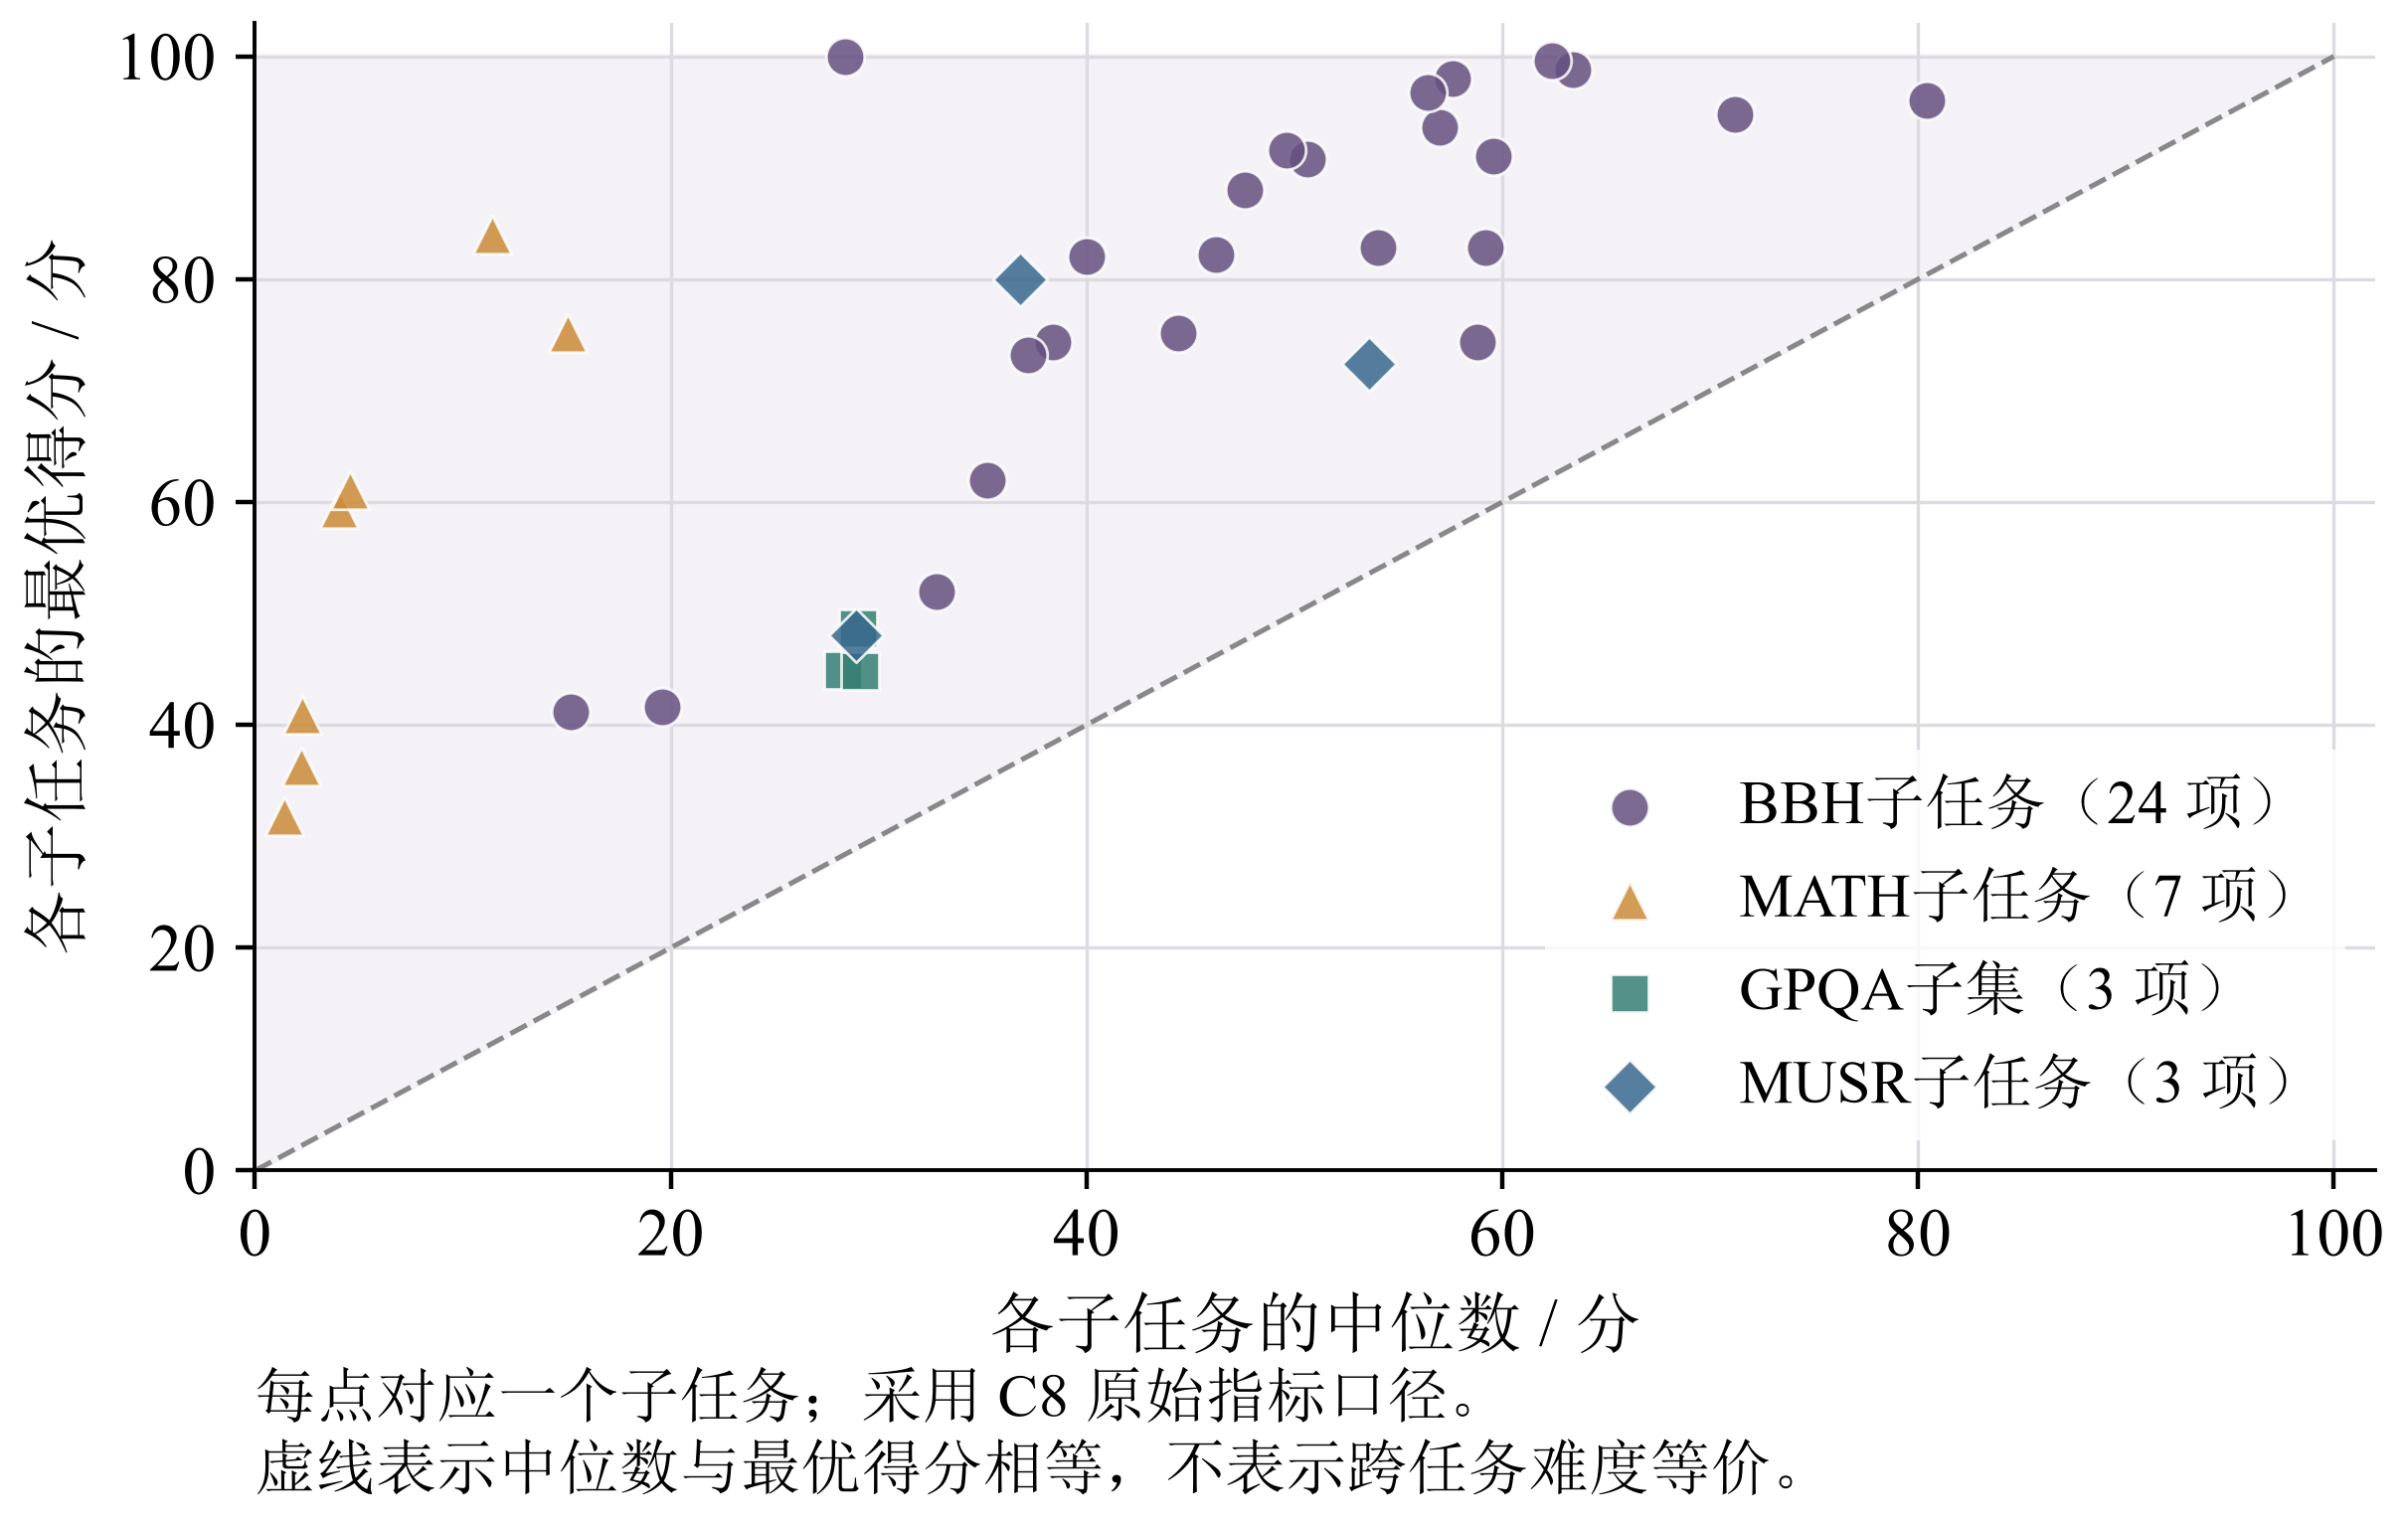
\includegraphics[width=0.98\textwidth]{../求解/问题四/图片/图4_逐任务聚合.png}
\caption{C8 的 37 个子任务表现：圆点、短线和菱形依次为中位数、前 $5\%$ 均值与最优得分；每项 $n=961\sim964$，采用原始指标口径}
\label{fig:p4_task}
\end{figure}

\begin{table}[!htbp]
\centering
\caption{距满分差值最大的六个子任务}
\label{tab:p4_sub}
\begin{tabularx}{0.98\textwidth}{@{}
>{\hsize=0.8\hsize\linewidth=\hsize\raggedright\arraybackslash}X
>{\hsize=2\hsize\linewidth=\hsize\raggedright\arraybackslash}X
>{\hsize=0.6\hsize\linewidth=\hsize\centering\arraybackslash}X
>{\hsize=0.9\hsize\linewidth=\hsize\centering\arraybackslash}X
>{\hsize=0.85\hsize\linewidth=\hsize\centering\arraybackslash}X
>{\hsize=0.85\hsize\linewidth=\hsize\centering\arraybackslash}X@{}}
\toprule
所属类别 & 子任务 & $n$ & \makecell{前 $5\%$\\均值} & 最优得分 & \makecell{距满分\\差值 / 分} \\
\midrule
MATH & 中级代数 & 962 & 20.11 & 31.79 & 68.2 \\
MATH & 预备微积分 & 962 & 22.89 & 36.30 & 63.7 \\
MATH & 几何 & 962 & 28.72 & 40.91 & 59.1 \\
BBH & 位置跟踪，7 个对象 & 964 & 32.67 & 41.20 & 58.8 \\
BBH & 位置跟踪，5 个对象 & 964 & 31.24 & 41.60 & 58.4 \\
GPQA & Extended 子集 & 961 & 39.74 & 44.87 & 55.1 \\
\bottomrule
\end{tabularx}
\end{table}

具体任务中，MATH-Hard 的中级代数、预备微积分和几何最高分在 $31.8\sim40.9$ 之间；BBH 的 5、7 对象位置跟踪约为 41 分；GPQA Extended 为 44.9 分。即便看各项最高表现，这些任务也仍有较大差距，可作为后续改进的关注对象。不过，各任务随机基线和难度不同，不能把原始分数当作完全相同的能力刻度。

按类别汇总，MATH 各任务最高分的均值为 55.5，全部模型和子任务观测合并后的中位数为 3.7；BBH 分别为 81.8、48.8。最高分均值可能由不同模型贡献，不表示某个模型同时达到这些值。结合任务内的分布，可以看出普通表现与单项前沿仍有差距，而不需要假定各任务的得分分布相同。

\subsubsection{宏观资源证据与预测边界}

最后使用 Epoch AI 数据库 C4\cite{epoch2025}观察训练算力、数据量及开放权重状态。它与 C1 规范化名称后只有 1 条匹配，无法组成有效的逐模型联合样本，因此单独用于宏观分析。图\ref{fig:p4_c4}依次给出 Language 领域年度算力范围、开放权重标记比例和 C4 全量字段覆盖，分别说明资源变化和资料完整性。

\begin{figure}[!htbp]
\centering
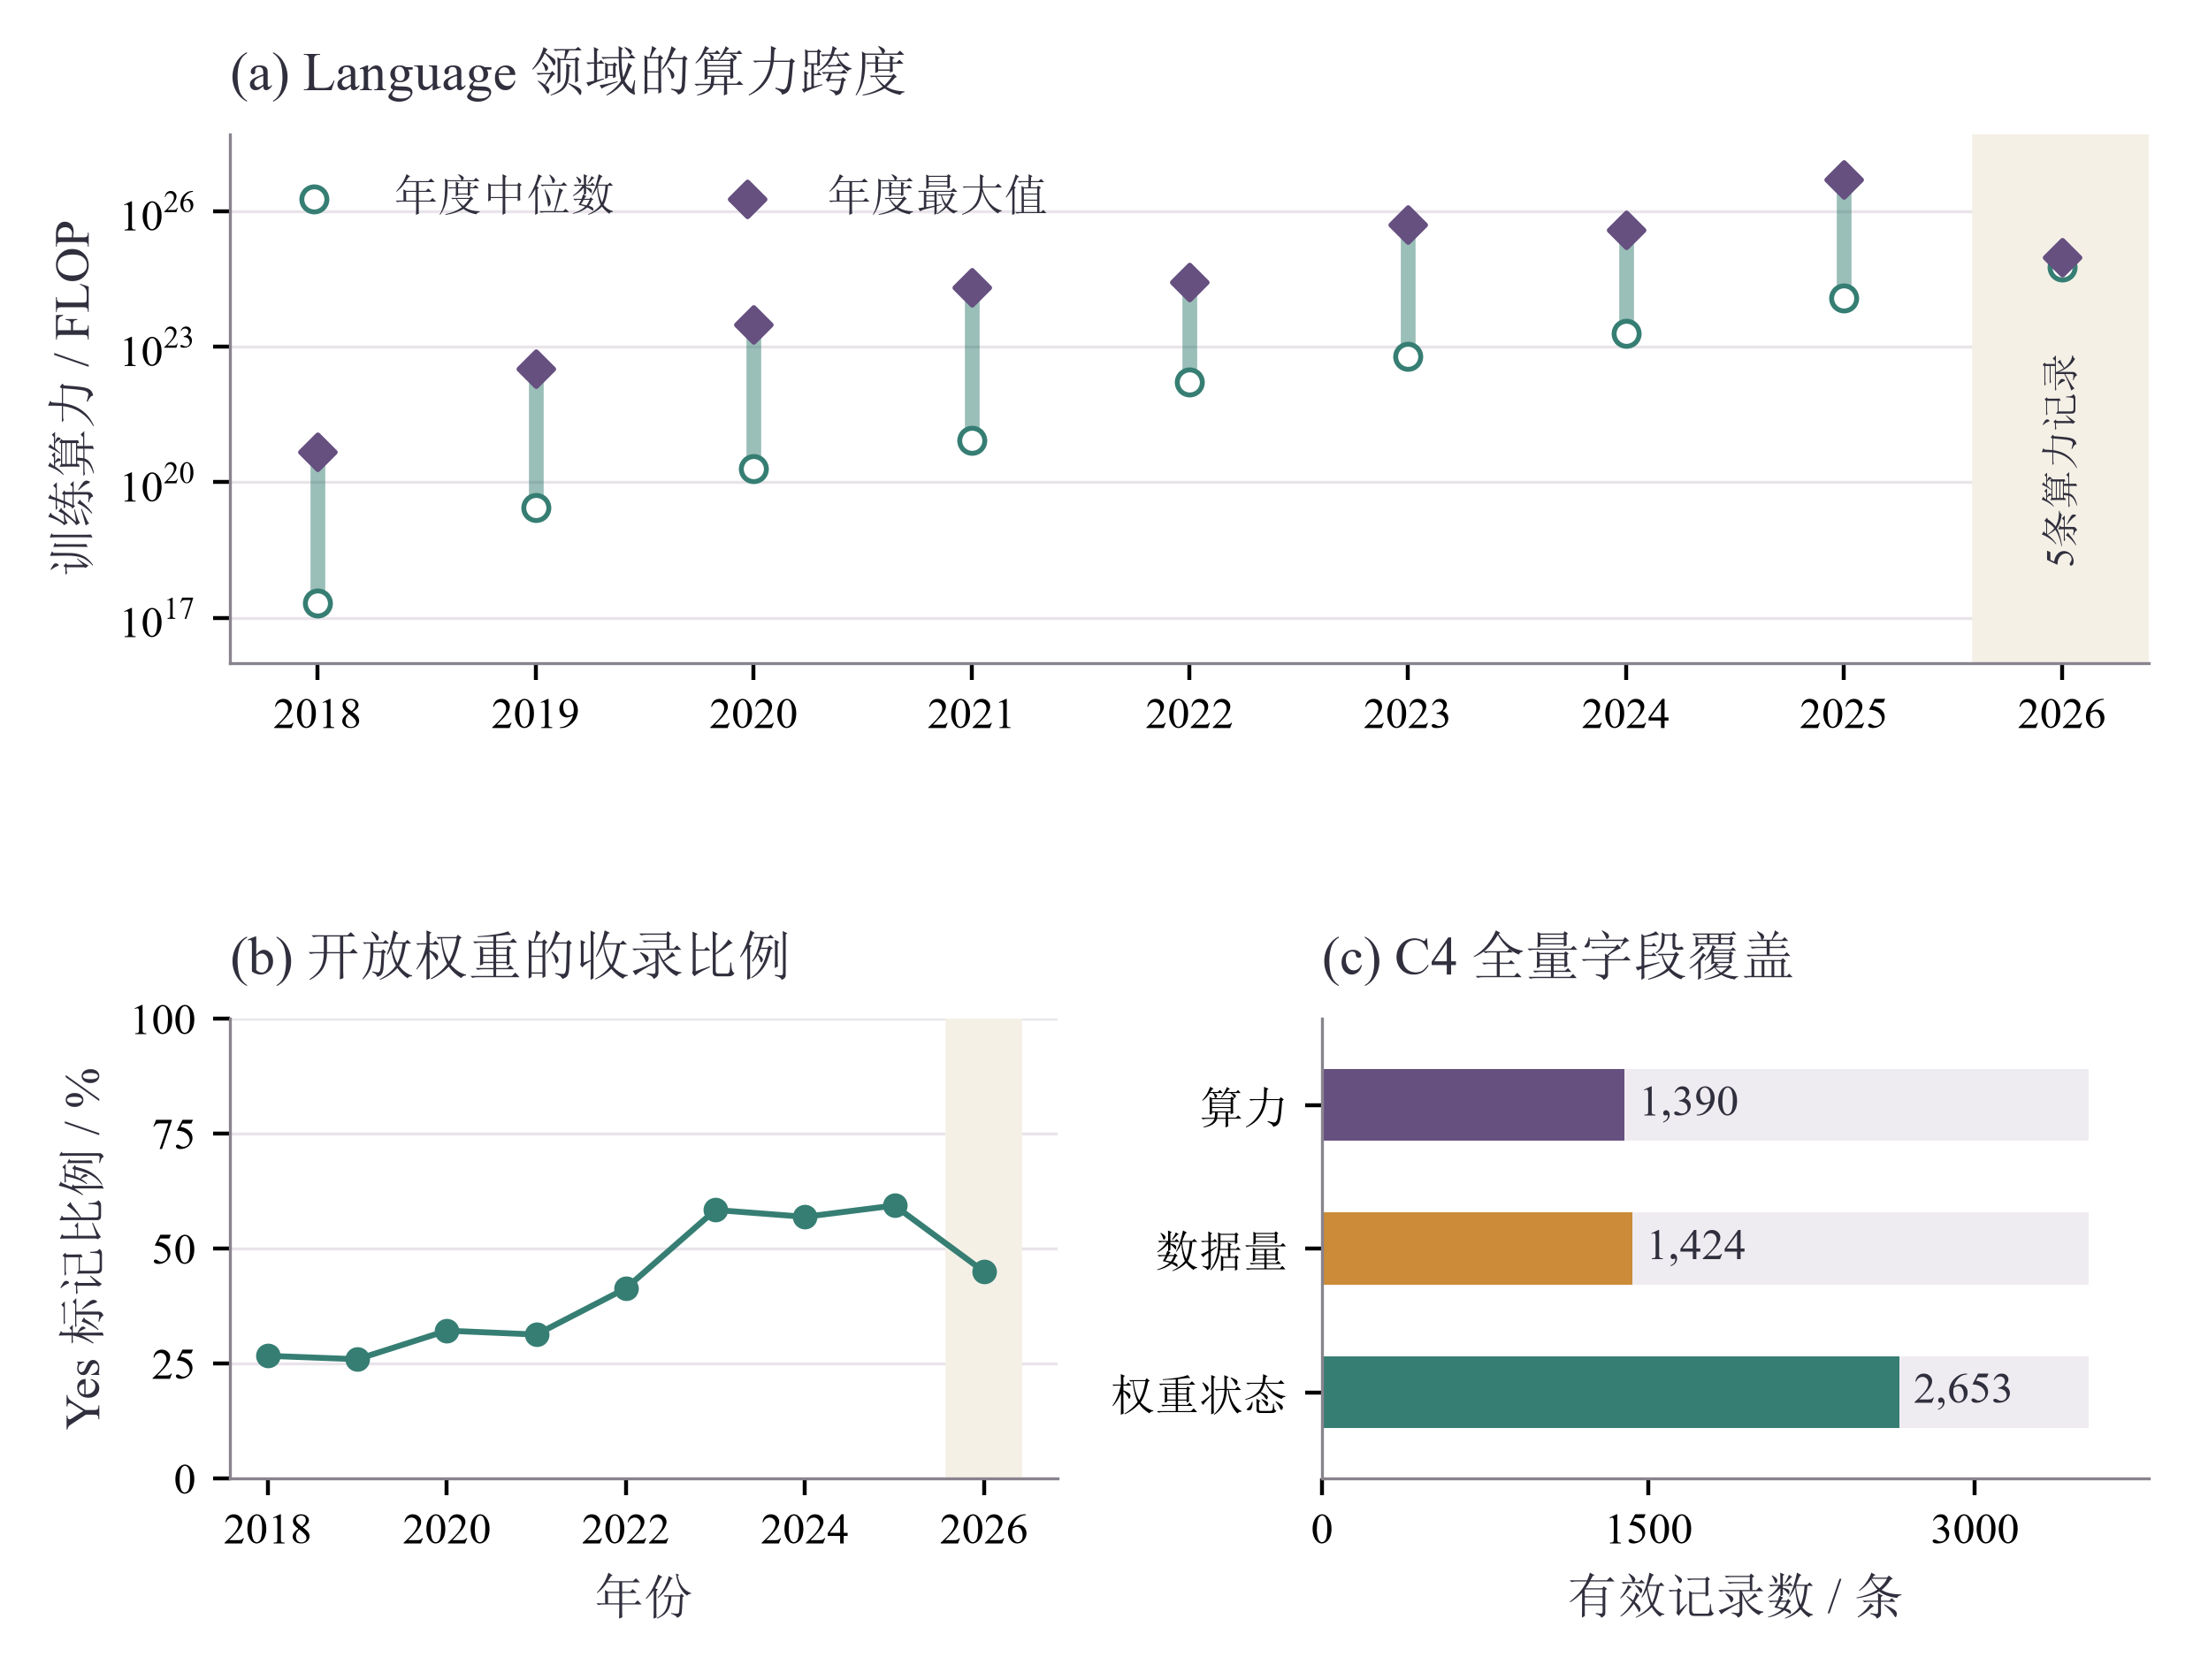
\includegraphics[width=0.98\textwidth]{../求解/问题四/图片/图5_C4宏观趋势.png}
\caption{C4 的资源演进与字段覆盖：上图连接每年算力中位数与最大值；左下为 Language 记录中权重标记 Yes 的比例；右下以全量 3{,}523 条记录为背景，浅色部分为字段缺失或状态未明确}
\label{fig:p4_c4}
\end{figure}

2018 至 2026 年，Language 子集共有 1{,}783 条记录。对九个年度的最大算力取对数拟合，年斜率约为 0.589 个数量级，即相邻年度的拟合算力之比约为 3.88。整体呈扩张趋势，但并不逐年增加，2024 年最大值低于 2023 年。2026 年目前只有 40 条 Language 记录，其中 5 条有算力值，该点容易受到收录不足影响，不能仅凭下降就判断技术趋势逆转。

Language 记录中，开放权重标记 Yes 的占比从 2018 年 26.7\% 变为 2025 年 59.4\%，中间也有下降。计算分母包含当年所有 Language 记录，其中包括权重状态缺失者。因此，该比例反映数据库的收录情况，不等于市场份额，也不足以证明 C1 对总体具有代表性。

C4 全量为 3{,}523 条，其中算力有值的为 1{,}390 条，训练数据量有值的为 1{,}424 条；权重状态明确的 2{,}653 条中，Yes 为 1{,}325，No 为 1{,}328。由于训练数据量缺失较多、来源也不统一，本节只报告其覆盖情况，不另估年度增长率。宏观变化可以帮助设置不同资源情景，但还不能确定算力放缓会使非规模进步按什么比例下降。

本问先确认了损失与能力之间的方向性联系，再分别核算长期和近期的前沿增量。长期样本中规模与非规模项大致各占一半，2024 年 6 至 9 月则主要为非规模项，两者需要按各自样本解释。未来预测同时保留曲线区间和结构情景的差异；具体能力改进则可重点观察数学、研究生级问答和多步推理等薄弱任务。

\FloatBarrier
\endgroup


% ════════════════════════════════════════════
% 模型检验与分析（6.模型检验.tex）写作规则 —— 模板内嵌，AI 先读本文件再写
% ════════════════════════════════════════════
\section{模型检验与分析}
\label{sec:validation}

我们从预测误差和条件变化两方面检验模型：前者考察对检验记录的预测，后者考察赋权、成本与预算改变后配置及结论是否保持。

\subsection{误差分析}
\label{sec:check}

表\ref{tab:error}汇总各问使用的检验指标。问题一的线性岭与核岭、问题二的经典和广义标度律，以及问题四的损失--得分桥接和合并横截面回归，分别报告 $R^2$、RMSE、MAE、MAPE。我们据此同时评价拟合解释度与预测偏差，避免仅凭相关性判断效果。

设同一评价集合中的观测值为 $y_i$，预测值为 $\hat y_i$，记录数为 $n$，均值为 $\bar y$。几类指标分别由残差的平方、绝对值及相对大小构成：
\begin{align*}
 R^2&=1-\frac{\sum_{i=1}^{n}(y_i-\hat y_i)^2}{\sum_{i=1}^{n}(y_i-\bar y)^2},\\
 \mathrm{RMSE}&=\sqrt{\frac{1}{n}\sum_{i=1}^{n}(y_i-\hat y_i)^2},\qquad
 \mathrm{MAE}=\frac{1}{n}\sum_{i=1}^{n}|y_i-\hat y_i|,\\
 \mathrm{MAPE}&=\frac{100\%}{n}\sum_{i=1}^{n}\left|\frac{y_i-\hat y_i}{y_i}\right|.
\end{align*}
其中，$R^2$ 需要观测值具有非零变异，MAPE 的逐条计算则要求观测值非零。RMSE 对较大的偏差给予更多权重，MAE 描述平均绝对偏离，两者与被预测量具有相同量纲；MAPE 便于阅读相对误差，但观测值靠近零时，少量记录也可能显著影响其大小。因此，我们结合样本取值范围共同报告这些指标。

我们还区分决定系数与相关系数的用途。$R^2$ 将残差与观测值围绕均值的变异作比较，要求预测值在实际尺度上接近观测值；Pearson 的 $r$ 则衡量两者共同变化的程度。预测序列整体偏高或偏低时，仍可能保持较高相关。表中的跨尺度相关用于评价趋势，其余结果按各问的评价集合解释，不据同列数值直接排列所有模型的优劣。

\begingroup
\setlength{\tabcolsep}{3pt}
\begin{longtable}{@{}>{\raggedright\arraybackslash}p{0.31\textwidth}>{\centering\arraybackslash}p{0.17\textwidth}>{\centering\arraybackslash}p{0.15\textwidth}>{\centering\arraybackslash}p{0.13\textwidth}>{\centering\arraybackslash}p{0.13\textwidth}@{}}
\caption{各问拟合、预测误差与预算约束残差汇总}\label{tab:error}\\
\toprule
  模型（数据集） & $R^2$ / $r$ 或残差 & RMSE / 相对残差 & MAE & MAPE(\%) \\
\midrule
\endfirsthead
\caption[]{各问拟合、预测误差与预算约束残差汇总（续）}\\
\toprule
  模型（数据集） & $R^2$ / $r$ 或残差 & RMSE / 相对残差 & MAE & MAPE(\%) \\
\midrule
\endhead
\bottomrule
\endfoot
问题一岭回归（训练 1M，$n=512$） & $R^2=0.629$ & 0.551 & 0.403 & 8.54 \\
  问题一岭回归（检验 1M，$n=256$） & $R^2=0.619$ & 0.523 & 0.386 & 8.43 \\
  问题一核岭（检验 1M，$n=256$） & $R^2=0.9454$ & 0.2256 & 0.1344 & — \\
  问题一跨尺度 Pearson（60M / 1B） & $r$: 0.782 / 0.651 & — & — & — \\
  问题二经典标度律（B1，$n=1{,}176$） & $R^2=0.9999998$ & $1.5\times10^{-4}$ & $1.1\times10^{-4}$ & 0.004 \\
  问题二经典标度律留出（4 小模型$\to$4 大模型） & $R^2=0.9999997$ & $1.5\times10^{-4}$ & — & 0.005 \\
  问题二广义标度律（B1+B6 联合，$n=1{,}536$） & $R^2=0.990$ & 0.036 & 0.017 & 0.66 \\
  问题二跨族验证（B4，$n=57$） & $r=0.975$ & 0.293 & — & 8.83 \\
  问题二文献验证（B5，$n=44$） & $r=0.910$ & 0.193 & — & 7.99 \\
  问题四 Loss—Benchmark 桥接（C6，$n=75$） & $R^2=0.26$ & — & — & 67.79 \\
  问题四合并横截面回归（C1 开源筛选，$n=2{,}346$） & $R^2=0.475$ & — & — & — \\
  问题四合并横截面回归（C3 长周期，$n=4{,}579$） & $R^2=0.424$ & — & — & — \\
  问题四前沿 logistic（历史拟合） & $R^2=0.975$ & — & — & — \\
  问题三优化约束残差（$|C_{\text{total}}/C_{\text{budget}}-1|$） & — & $<10^{-6}$ & — & — \\
\end{longtable}
\endgroup

问题一的同尺度预测与训练表现接近。表\ref{tab:error}中，13 个验证域的平均训练 $R^2$ 为 $0.629$，1M 检验为 $0.619$，相差 $0.010$，MAPE 约 $8.5\%$。这一对照没有显示明显的训练与检验落差，但不能据此排除线性欠拟合。核岭的同尺度平均域 $R^2=0.9454$、综合 RMSE 为 $0.2256$；相应训练五折误差为 $0.2558$。跨尺度绝对误差见表\ref{tab:p1_nonlinear}，较高趋势相关不代表绝对损失准确。

问题二的精度取决于检验来源。对 B1，经典拟合有 $R^2\approx1.000$、MAPE $0.004\%$，仅用小模型估计后，对大模型的留出预测仍有 $R^2=0.9999997$；残差标准差 $1.5\times10^{-4}$ 相比损失标准差 $0.342$ 很小。这些结果说明对 B1 的贴合程度高，尚不能说明跨来源同样准确。B4 和 B5 的 MAPE 分别为 $8.8\%$、$8.0\%$，相关分别为 $r=0.975$、$r=0.910$。广义模型的 $1{,}536$ 条联合记录给出 $R^2=0.990$、MAPE $0.66\%$；由于样本组成改变，不能将其拟合优度与经典模型直接作差来判断泛化收益。

问题四的换算精度主要受样本可比性限制：中可比层的验证集不同，高可比层的得分跨度有限，合并后的 $R^2=0.26$、MAPE 为 $67.8\%$，故结果仅作方向解释。问题三检查的是预算可行性；表中最后一行的数值是成本回代得到的相对预算残差，虽与 RMSE 同列展示，不能解释为预测误差。有效解的残差均 $<10^{-6}$，符合成本约束。

各问的评价集合不同，也决定了误差数字的使用范围。问题一的检验针对新配方下的领域损失，问题二的对照涉及不同规模、质量和资料来源，问题四的桥接还要跨越损失与能力两种指标。较小误差能够支持相应集合内的描述，却不能自动扩大到其他来源。因此，我们按记录来源及其是否参与估计，限定表\ref{tab:error}中各项误差的解释范围。

预算约束残差与上述预测误差的含义不同。残差接近零，说明返回的参数量、数据量和质量在给定成本式下基本用尽预算；它本身不衡量标度律的预测精度，也不说明外部评测得分会提高多少。因此，我们从预算可行性、预测损失和资源份额三个方面评价问题三的配置。

\subsection{灵敏度分析}
\label{sec:sensitivity}

表\ref{tab:sensitivity}比较赋权方式、冲突阈值、岭正则、质量成本、质量基线、上下文长度和预算变化后的结果，同时补充指标方向与跨来源验证的影响。我们通过这些对照识别较稳定的结论，以及依赖特定成本或样本的结论。

\begin{longtable}{@{}>{\raggedright\arraybackslash}p{0.30\textwidth}>{\raggedright\arraybackslash}p{0.36\textwidth}>{\raggedright\arraybackslash}p{0.26\textwidth}@{}}
\caption{评分规则、成本与预算变化下的结果稳定性}\label{tab:sensitivity} \\
\toprule
参数/设定变化 & 输出变化 & 灵敏度评估 \\
\midrule
\endfirsthead
\caption[]{评分规则、成本与预算变化下的结果稳定性（续）} \\
\toprule
参数/设定变化 & 输出变化 & 灵敏度评估 \\
\midrule
\endhead
\midrule
\multicolumn{3}{r}{续下页} \\
\endfoot
\bottomrule
\endlastfoot
赋权方案：熵权法 $\to$ 等权平均 $\to$ 首主成分非负载荷加权 & 域级质量排序一致性 $0.643\to0.679$；样本级得分相关 $0.875/0.927$；得分均值 $0.491\to0.637\to0.496$ & 中等敏感：整体格局稳定，但领域名次会变化 \\
  指标方向：ad\_en 按“索引 1=无广告”（正向）$\to$ 若误判为负向 & 领域质量排序由「arxiv $>$ stackexchange $>$ c4 $>$ commoncrawl $>$ book $>$ wikipedia $>$ github」变为「c4 $>$ arxiv $>$ commoncrawl $>$ stackexchange $>$ book $>$ wikipedia $>$ github」 & 高度敏感：方向判定必须用实证证据 \\
  冲突阈值 $\tau$：$0.5\to1.0\to1.5\to2.0\to2.5$ & 冲突率 $0.657\to0.394\to0.219\to0.120\to0.066$；与独立基准之比 $0.91\to0.82\to0.76\to0.76\to0.86$ & 结论稳健：所考察阈值下冲突率均低于独立基准 \\
  岭正则系数 $\lambda$：$10^{-4}\sim10^{-1}$ & 训练 $R^2$ 由 $0.6291$ 降至 $0.6238$，检验 $R^2$ 由 $0.6187$ 降至 $0.6157$ & 拟合精度较稳定；系数与候选配比仍会变化 \\
  质量成本函数：指数型 $\to$ 幂函数型 $\to$ 对数渐进型（$C=10^{19}$） & $Q^{*}=0.660\to0.549\to1.000$，$L^{*}$ 差异 $<0.06$；质量份额 $13.1\%\to0.0\%\to31.7\%$ & 低预算档较敏感 \\
  同上，考察 $C=10^{22}$、$10^{24}$ & 三种函数下 $Q^{*}$ 均为 $1.000$；在 $10^{22}$ 档，$D^{*}$ 为 229.4--274.1B tokens，最大值较最小值高约 $19.5\%$ & 质量均达到上界，规模配置仍有差异 \\
  质量基线口径：配比加权 $Q_0=0.5487\to$ 样本均值 $0.4912$ & 三档预算下 $Q^{*}$：$0.549/1.000/1.000\to0.507/1.000/1.000$，低预算质量份额由 $0$ 变为 $2.63\%$，$N^{*}$ 最大变化约 $3.24\%$ & 规模配置变化较小；低预算是否启动质量投入依赖基线口径 \\
  上下文长度：$2{,}048\to131{,}072$ tokens（C7 可行取值） & 注意力/训练倍数 $0.07\to4.37$；$N^{*}$ 由 $6.091$B 降至 $2.705$B；损失上升 $6.0\%$ & 对配置影响较大；$L_{\text{crit}}=30{,}000$ 为两项成本相等的位置 \\
  算力预算 $C$：$10^{19}\to10^{24}$ FLOPs & $Q^{*}$ 由 $0.549$ 升至 $1.000$；$D^*/N^*$ 由 $30.9$ 升至 $76.1$；质量份额 $0\to0.407\to0.016$ & 本成本与质量曲率下出现三个投入阶段 \\
  半合成数据验证：B2 / B8 & B2 的 MAPE 为 $33.7\%$；B8 校准段翻转质量方向后为 $133.4\%$，其部分数据损失低于本模型的参考渐近损失基准 & 跨来源偏差较大，两者均未参与主拟合 \\
\end{longtable}

表\ref{tab:sensitivity}显示，不同设定对结果的影响程度并不相同。

我们按条件作用的位置解释这些差异。调整权重或指标方向，会先改变质量评分；调整质量费用和上下文长度，会改变预算中各项支出的比例；扩大总预算，则是在同一成本形式下改变可配置的资源总量。因而，我们除比较最终损失外，也比较中间变量和配置份额。若两种方案的预测损失接近，但质量份额相差较大，就说明目标值相近并不要求投入方式相同。

阈值、正则参数和预算扫描均由有限取值构成。相邻取值下的结果可用来判断已检验范围内的变化方向，首次发生变化的网格点则给出定位边界的线索。我们保留扫描间距和求解状态，并结合费用关系解释变化。图中连接相邻点仅用于展示趋势，未检验区间不具有与扫描点相同的数值依据。

\textbf{（1）较稳定的结果。} 在所检验阈值内，冲突率始终低于独立参照，比值均 $<0.92$。岭正则变化对拟合精度影响较小；更换质量基线后，规模配置变化较小，但低预算是否启动质量投入随基线口径改变。三类成本在所考察的中高预算档都使质量达到上界，但参数量、数据量的具体组合仍然不同。

\textbf{（2）需要区分的边界。} $L_{\text{crit}}=30{,}000$ tokens 只表示注意力费用与基础训练费用相等，不代表最优解在此处发生突变；$1.58\times10^{19}$、$7.08\times10^{19}$ FLOPs 是预算网格中首次出现质量投入和首次达到上界的有效点，实际边界还受网格间距、求解状态及成本形式影响。

\textbf{（3）依赖条件的结果。} $C=10^{19}$ FLOPs 下更换质量成本时，最优质量覆盖 $0.549\sim1.000$，说明低预算策略依赖成本设定，应同时比较各情景；损失--得分桥接只有 $R^2=0.26$，不能精确换算能力分；领域排序也会受指标方向和赋权方式影响。

补充检验进一步区分了拟合精度与决策稳定性。问题一在同一个加权损失目标下比较线性岭与核岭，见表\ref{tab:q1_review_target}及表\ref{tab:q1_review_surrogates}，发现原线性候选的相对收益方向随响应函数而变；正则变化对平均 $R^2$ 的影响虽小，系数符号和领域份额仍会变化，见表\ref{tab:q1_review_ridge}。问题二、三的表\ref{tab:q23_review_quality_scale}和表\ref{tab:q23_review_gamma}分别检查质量映射与曲率：保持质量排序不变仍会改变边际收益，而将 $\gamma$ 固定为 1 时，拟合目标只增加约 $0.024\%$，原首次饱和预算下的最优质量降至约 $0.964$。因此，精度相近不足以证明端点配置稳定。

表\ref{tab:q23_review_m_amplitude}则将配比修正的迁移幅度从零逐步提高到原值。等效预算倍数随之从 1 增至约 29.6，说明该量主要反映配比收益的迁移假设；它不能单独作为真实训练节省的估计。以上对照均另存为诊断输出，原拟合参数和正式配置结果保持不变。

问题四的表\ref{tab:q4_review_time}显示，年份组差对同名去重较稳定，但含义仍是不同模型记录之间的条件差异。表\ref{tab:q4_review_window}和表\ref{tab:q4_review_holdout}进一步表明，前沿曲线的饱和位置对平台窗口敏感，所选时间留出期的误差也高于保持最后峰值的参照。这项事后检查不足以选定一个普遍更优的预测方法，但足以说明全样本拟合度不能替代时间外验证。

\subsection{各问结果的衔接与使用条件}

完成单项检验后，我们进一步核对结果在各问之间的传递。质量基线、配比修正和标度律参数对下一问的作用不同，因此分别检查其影响位置与使用条件，明确现有检验覆盖的范围。

质量基线 $Q_0$ 一方面确定问题三的质量起点，另一方面进入增量费用 $[g(Q)-g(Q_0)]_+$。所以，更换基线会同时改变质量可选区间和费用参照，不能仅把结果表中的质量数值平移后仍视为同一方案。前述两种基线的对照已经给出相应配置；我们将各自基线、成本形式及配置共同列为使用条件。问题一中缺少直接领域质量观测的部分，也需要随映射规则一并说明。

配比修正 $M(\bm p)$ 则以损失平移量进入广义模型。配比固定时，它不参与参数量、数据量和质量的求导，但仍影响报告的预测损失水平。因而，讨论规模配置与讨论配方收益时，需要明确是否沿用同一配比。问题一的有界候选在不同响应函数下收益方向不同，问题二的跨来源对照也未完成配比响应的数值标定，因此配方收益及其算力等价只作为条件情景。

标度律参数决定不同投入的边际收益，成本函数决定实现这些投入要支出多少算力。问题二的拟合误差与问题三的成本敏感性分别考察这两侧的关系。现有结果可以说明给定参数和成本下怎样配置，也可以比较已设定成本情景之间的差别；对于参数误差与成本误差同时变化后的影响，本文没有另外给出联合概率区间，因此不把这些情景差别解释成最优配置的置信范围。

能力预测又使用另一组观测。损失--得分桥接展示了两类指标的关联程度，历史前沿和合并横截面回归则直接使用评测记录。问题三中的损失下降据此解释为训练目标的改善，问题四的能力增量保留为相应评测尺度下的结果；两者均应结合各自的样本范围和桥接假设解读。

% ════════════════════════════════════════════
% 模型的评价（7.模型评价.tex）写作规则 —— 模板内嵌，AI 先读本文件再写
% ════════════════════════════════════════════
\section{模型的评价}

\subsection{模型的优点}
\begin{itemize}[itemindent=2em]
\item \textbf{质量评分有明确依据。} 表\ref{tab:p1_dir}逐项说明 22 个指标的方向，广告字段还通过原文抽查确认“第 1 类=无广告”。处理时将负向指标反向转换、长度指标转为中心接近度，8 个列表指标通过 softmax 期望压缩，并用中位数填补 19 处缺失。抽样与扩展集合的可比领域差值约为 $0.002$，为这两类数据上的评分一致性提供了对照。
\item \textbf{指标冲突可以相对比较。} 本文同时给出 $22.3\%$ 的冲突率、$0.069$ 的 Kendall 系数和 $28.9\%$ 的独立参照。在 $\tau\in[0.5,2.5]$ 的检验范围，比值均 $<0.92$。这样可以区分“存在共同倾向”与“高度一致”，再结合三类分歧原因和处理规则解释冲突样本。
\item \textbf{质量项便于解释和比较。} $C(1-Q)^{\gamma}$ 在 $Q=1$ 时归零，恢复 Chinchilla 的函数形式；与直接使用 $E-CQ^{\gamma}$ 相比，不会因减去质量项而在高质量端出现负损失。模型选择比较了四种形式的 $R^2$、残差信息评分及范围内外表现。B3 插值轨迹的数据指数约为 $-0.2805$，与 $-0.2799$ 接近，提供了内部一致性检查。
\item \textbf{配置变化可从成本公式解释。} 模型保留 $C_Q=D[g(Q)-g(Q_0)]_+$，使质量费用随处理的数据量变化，并使用题设附录 B 的三类函数参数。由此求得 $L_{\text{crit}}=6/\eta=30{,}000$，并推导式\eqref{eq:p3_balance}。折算量 $\tau(Q)$ 将质量费用换成与参数量相同的单位，便于理解质量投入如何改变参数与数据的平衡。
\item \textbf{不同来源的结果分别解释。} 问题四列明许可、时间变量和模型类型，在 C8 的 $1{,}860$ 个有效目录中，用主样本交集的 $964$ 个目录汇总 $37$ 项任务；六维指标另与完整 C1 作名称匹配和记录级秩相关检查。C4 用于宏观资源及字段覆盖分析，预测中区分重抽样区间和情景范围。对 B2/B8 的异常也保留检验说明，例如 B8 存在低于不可约损失下限的记录，避免把不同性质的数据当作同等证据。
\end{itemize}

\subsection{模型的缺点}
\begin{itemize}[itemindent=2em]
\item \textbf{配比关系仍是线性近似。} 模型没有领域交互项，13 个验证域的平均 $R^2$ 为 $0.629$，约 $37\%$ 的变异仍未解释，可能还与随机种子、数据顺序等因素有关。nih\_exporter、enron\_emails、europarl、philpapers 缺少自身损失列，优化时固定在参考占比，难以单独判断其影响。混合质量指数只带来 $9.9\times10^{-5}$ 的 $R^2$ 增量，说明当前线性组合没有提供明显的新信息，也限制了进一步利用 17 域评分细化配方的空间。
\item \textbf{部分评分方向仍依赖字段含义。} 广告、流畅度已用原文及领域对照检查，但 modernbert 的 6 级指标、qurater 的 4 级评级等，仍按“高等级对应高质量”的语义处理，缺少独立验证。熵权也受到分布形态影响，改用等权后领域排序一致性为 $0.679$。第\ref{sec:check}节还显示，方向误判会明显改变排名，因此排名细节应与方向和赋权方法一起解释。
\item \textbf{质量实验的支持范围有限。} 质量项主要依靠 B6/B7 半合成实验，B8 方向相反且含低于损失下限的记录，不能并入主拟合；B2 的 MAPE 为 $33.7\%$，也说明跨来源估计仍有较大偏差。质量配置只在 $[Q_0,1]$ 内讨论，更低质量的外推尚缺数据支持。
\item \textbf{能力预测受到时间和评分限制。} 损失映射的 $R^2=0.26$、MAPE 为 $67.8\%$，不能精确换算收益。C1 可比窗口约 10 个月，预测却长达其 $1.2\sim2.4$ 倍，C3 历史评测又存在来源差异。两个年份的回归不足以识别具体技术机制，非规模项还包含样本构成等因素。因此，长期规模占比 $50.5\%$ 与 2024 年 6—9 月的 $4.6\%$ 只能分别对应各自窗口。
\end{itemize}

% ════════════════════════════════════════════
% 模型的改进与推广（8.模型改进推广.tex）写作规则 —— 模板内嵌，AI 先读本文件再写
% ════════════════════════════════════════════
\Needspace{10\baselineskip}
\section{模型的改进与推广}

\subsection{模型的改进}

后续改进可围绕当前尚未解释的差异、成本设定和数据覆盖展开。

在配比模型中，可对占比变量作适当变换，并加入领域交互项，再用 Group Lasso 等方法控制新增项数量，以考察 13 个领域平均 $R^2=0.629$ 之外约 $37\%$ 的变异。对于 nih\_exporter 等四个缺少验证损失的领域，可补充文本统计特征作为代理信息，减少固定参考占比的限制。冲突处理也可尝试有序 probit 因子模型，用共同的潜在质量解释指标分歧，进一步估计可信区间。

在质量模型中，可检验 $C(1-Q)^{\gamma_1}D^{-\gamma_2}$ 或其他质量与数据量交互形式，判断质量缺口是否会随数据规模变化。资源配置还可加入重复训练轮次、稀疏化与量化下的训练和推理费用，以及分阶段课程学习。针对低预算结果对成本形式较敏感的问题，更直接的办法是记录真实清洗流程的费用，拟合经验成本曲线后再与三类题设函数比较。

数据补充应优先服务于这些检验。可收集带质量标注的公开语料，扩展 B6/B7 目前覆盖的质量范围，并检查发布时间、许可、去重比例等信息能否辅助解释质量标签。C4 与 C1 可结合组织名、参数量和发布时间尝试匹配，经核实后再用于训练算力与能力的联合分析。若能获得 v1、v2 评测的共同校准样本，还可把 2019--2023 的历史记录换到同一尺度，减少当前可比窗口只有 10 个月的限制。

\subsection{模型的推广}

本文的方法可用于其他需要在有限成本下比较多项投入的场景，但应用前应重新检查数据、损失函数和成本关系。

在大模型预训练、微调和蒸馏中，可以沿用先拟合损失、再核算成本、最后优化配置的步骤。式\eqref{eq:p3_balance}和 $\tau(Q)$ 提供了比较语料处理与规模投入的方法；用于新任务时仍需重新估计对应参数，才能判断达到目标表现需要多少算力。

在语料治理中，22 个指标的方向表及冲突率相对独立参照的比较，可帮助开展文本筛选、清洗和配比调整。领域系数相似度 $s_{ij}$ 则可辅助寻找作用接近或不同的语料来源。具体能否等量替换、混合后是否有额外收益，仍应通过配比实验确认。

在科研资源规划中，可借鉴长周期 shift-share 分解与近期同一评测窗口对照的做法，分别观察扩参数与其他变化对应的增量。它能提供投入分析的线索，但非规模项不能全部归为算法收益。区分稳定结果、阶段边界和受假设影响较大的结果，也有助于多来源数据分析中的决策使用。

对于芯片制程、新能源和生物医药等可能逐渐趋于饱和的技术指标，也可比较 logistic 曲线与结构情景的预测差异，前提是先验证该指标确有相应增长特征。使用半合成或估算资料时，本文对评分方向和不可约损失下限的检查也可作为参考，帮助识别不能直接混合分析的数据。

\begin{thebibliography}{99}
\raggedright
\setlength{\emergencystretch}{2em}

\bibitem{kaplan2020scaling} KAPLAN J, MCCANDLISH S, HENIGHAN T, et al. Scaling laws for neural language models[EB/OL]. (2020-01-23)[2026-09-27]. \url{https://arxiv.org/abs/2001.08361}.

\bibitem{hoffmann2022chinchilla} HOFFMANN J, BORGEAUD S, MENSCH A, et al. An empirical analysis of compute-optimal large language model training[C]//Advances in Neural Information Processing Systems. Curran Associates, 2022, 35: 30016-30030.

\bibitem{besiroglu2024replication} BESIROGLU T, ERDIL E, BARNETT M, et al. Chinchilla scaling: A replication attempt[EB/OL]. (2024-04-15)[2026-09-27]. \url{https://arxiv.org/abs/2404.10102}.

\bibitem{villalobos2022data} VILLALOBOS P, HO A, SEVILLA J, et al. Position: Will we run out of data? Limits of LLM scaling based on human-generated data[C]//Proceedings of the 41st International Conference on Machine Learning. PMLR, 2024, 235: 49523-49544.

\bibitem{gunasekar2023textbooks} GUNASEKAR S, ZHANG Y, ANEJA J, et al. Textbooks are all you need[EB/OL]. (2023-06-20)[2026-09-27]. \url{https://arxiv.org/abs/2306.11644}.

\bibitem{li2024datacomp} LI J, FANG A, SMYRNIS G, et al. DataComp-LM: In search of the next generation of training sets for language models[C]//Advances in Neural Information Processing Systems. Curran Associates, 2024, 37: 14200-14282.

\bibitem{liu2024regmix} LIU Q, ZHENG X, MUENNIGHOFF N, et al. RegMix: Data mixture as regression for language model pre-training[C/OL]//The Thirteenth International Conference on Learning Representations. 2025[2026-09-27]. \url{https://openreview.net/forum?id=5BjQOUXq7i}.

\bibitem{gao2020pile} GAO L, BIDERMAN S, BLACK S, et al. The Pile: An 800GB dataset of diverse text for language modeling[EB/OL]. (2020-12-31)[2026-09-27]. \url{https://arxiv.org/abs/2101.00027}.

\bibitem{slimpajama2025} OPENDATALAB. SlimPajama-Meta-rater[DB/OL]. [2026-09-27]. \url{https://huggingface.co/datasets/opendatalab/SlimPajama-Meta-rater}.

\bibitem{shannon1948} SHANNON C E. A mathematical theory of communication[J]. Bell System Technical Journal, 1948, 27(3): 379-423. DOI: 10.1002/j.1538-7305.1948.tb01338.x.

\bibitem{kendall1939} KENDALL M G, SMITH B B. The problem of $m$ rankings[J]. The Annals of Mathematical Statistics, 1939, 10(3): 275-287. DOI: 10.1214/aoms/1177732186.

\bibitem{hoerl1970ridge} HOERL A E, KENNARD R W. Ridge regression: Biased estimation for nonorthogonal problems[J]. Technometrics, 1970, 12(1): 55-67. DOI: 10.1080/00401706.1970.10488634.

\bibitem{sklearn_krr} SCIKIT-LEARN DEVELOPERS. Kernel ridge regression[EB/OL]. [2026-09-27]. \url{https://scikit-learn.org/stable/modules/kernel_ridge.html}.

\bibitem{ai_workbuddy} 腾讯. WorkBuddy：AI 办公工作台[EB/OL]. [2026-09-27]. \url{https://cloud.tencent.com/product/workbuddy}.

\bibitem{ai_deepseek} DEEPSEEK. DeepSeek-V4-Flash（公开测试）[EB/OL]. (2026-07-31)[2026-09-27]. \url{https://api-docs.deepseek.com/updates}.

\bibitem{ai_codex56luna} OPENAI. Codex（模型：GPT-5.6-Luna）[EB/OL]. (2026-07-09)[2026-09-27]. \url{https://developers.openai.com/api/docs/models/gpt-5.6-luna}.

\bibitem{biderman2023pythia} BIDERMAN S, SCHOELKOPF H, ANTHONY Q G, et al. Pythia: A suite for analyzing large language models across training and scaling[C]//Proceedings of the 40th International Conference on Machine Learning. PMLR, 2023, 202: 2397-2430.

\bibitem{scipy_slsqp} SCIPY DEVELOPERS. minimize(method=SLSQP)[EB/OL]. [2026-09-27]. \url{https://docs.scipy.org/doc/scipy/reference/optimize.minimize-slsqp.html}.

\bibitem{xie2023doremi} XIE S M, PHAM H, DONG X, et al. DoReMi: Optimizing data mixtures speeds up language model pretraining[C]//Advances in Neural Information Processing Systems. Curran Associates, 2023, 36: 69798-69818.

\bibitem{muennighoff2023scaling} MUENNIGHOFF N, RUSH A, BARAK B, et al. Scaling data-constrained language models[C]//Advances in Neural Information Processing Systems. Curran Associates, 2023, 36: 50358-50376.

\bibitem{schaeffer2023mirage} SCHAEFFER R, MIRANDA B, KOYEJO S. Are emergent abilities of large language models a mirage?[C]//Advances in Neural Information Processing Systems. Curran Associates, 2023, 36: 55565-55581.

\bibitem{openllm2025} HUGGING FACE. Open LLM Leaderboard results[DB/OL]. [2026-09-27]. \url{https://huggingface.co/datasets/open-llm-leaderboard/results}.

\bibitem{zhou2023ifeval} ZHOU J, LU T, MISHRA S, et al. Instruction-following evaluation for large language models[EB/OL]. (2023-11-14)[2026-09-27]. \url{https://arxiv.org/abs/2311.07911}.

\bibitem{wang2024mmlupro} WANG Y, MA X, ZHANG G, et al. MMLU-Pro: A more robust and challenging multi-task language understanding benchmark[C]//Advances in Neural Information Processing Systems. Curran Associates, 2024, 37: 95266-95290.

\bibitem{efron1979bootstrap} EFRON B. Bootstrap methods: Another look at the jackknife[J]. The Annals of Statistics, 1979, 7(1): 1-26. DOI: 10.1214/aos/1176344552.

\bibitem{epoch2025} EPOCH AI. Data on AI models[DB/OL]. [2026-09-27]. \url{https://epoch.ai/data/ai-models}.

\bibitem{ai_rules2026} 中国研究生数学建模竞赛组织委员会, 中国研究生数学建模竞赛专家委员会. “华为杯”第二十三届中国研究生数学建模竞赛人工智能工具及输出使用规定[EB/OL]. (2026-09-16)[2026-09-27]. \url{https://cpipc.acge.org.cn/sysFile/downFile.do?fileId=4fc024f7a1504abb87fc056440c64a28}.

\end{thebibliography}

\clearpage
\makeatletter
\let\@oldaddcontentsline\addcontentsline
\renewcommand{\addcontentsline}[3]{}

\section*{附录}
\let\addcontentsline\@oldaddcontentsline
\makeatother

\renewcommand{\arraystretch}{1.2}

\subsection*{附录 A：数据利用清单}

附录 A 按附件编号说明每份数据在本文中的用途，并把真实记录、半合成实验、插值轨迹和外推估算区分开来。这样既方便复核文件与结果的对应关系，也能看出哪些结论来自直接观测，哪些只用于对照或稳健性检查，详见表\ref{tab:appendix}。

\begin{longtable}{@{}>{\centering\arraybackslash}p{0.09\textwidth}>{\raggedright\arraybackslash}p{0.23\textwidth}>{\centering\arraybackslash}p{0.08\textwidth}>{\centering\arraybackslash}p{0.08\textwidth}>{\raggedright\arraybackslash}p{0.40\textwidth}@{}}
  \caption{附件数据利用清单}
  \label{tab:appendix} \\
  \toprule
  编号 & 文件名 & 性质 & 是否使用 & 使用方式与可信度说明 \\
  \midrule
  \endfirsthead
  \caption{附件数据利用清单（续）} \\
  \toprule
  编号 & 文件名 & 性质 & 是否使用 & 使用方式与可信度说明 \\
  \midrule
  \endhead
  \bottomrule
  \endfoot
  A1 & slimpajama\_\allowbreak{}quality\_\allowbreak{}signal\_\allowbreak{}sample & 真实 & 使用 & 对全量 51{,}230 条计算 22 指标熵权评分、领域 $Q$ 与冲突，并抽查原文 \\
  A2 & slimpajama\_\allowbreak{}quality\_\allowbreak{}extended/arxiv & 真实 & 使用 & 以全部 17{,}523 条计算 arxiv 的领域 $Q$，与抽样结果比较 \\
  A3 & slimpajama\_\allowbreak{}quality\_\allowbreak{}extended/github & 真实 & 使用 & 以全部 203{,}752 条计算 github 的领域 $Q$，与抽样结果比较 \\
  A4 & train\_\allowbreak{}mixture\_\allowbreak{}1m & 真实 & 使用 & 512 组训练配方作为岭回归输入，用于拟合配比与损失 \\
  A5 & train\_\allowbreak{}pile\_\allowbreak{}loss\_\allowbreak{}1m & 真实 & 使用 & 提供回归对应的 13 个验证域损失 \\
  A6--A9 & test\_\allowbreak{}mixture/loss\_\allowbreak{}1m, 60m & 真实 & 使用 & 分别检验同尺度和跨尺度的预测，每组 256 条 \\
  A10--A11 & test\_\allowbreak{}mixture/loss\_\allowbreak{}1B & 真实 & 使用 & 用 64 组记录检验跨尺度的预测 \\
  A12--A15 & est\_\allowbreak{}mixture/loss\_\allowbreak{}10b, 70b & 子集/外推 & 使用 & 各 63 组用于比较外推尺度因子的稳定性；属于外推记录，并非观测 \\
  A16 & domain\_\allowbreak{}mapping\_\allowbreak{}guide & 参考 & 使用 & 连接 17 域与质量分类：6 域按 direct/near\_\allowbreak{}direct 对应，11 域标为 inferred 并使用全局均值 \\
  A17 & regmix\_\allowbreak{}domain\_\allowbreak{}summary & 真实 & 未使用 & 未用于本文分析 \\
  A18 & regmix\_\allowbreak{}domain\_\allowbreak{}sample & 真实 & 未使用 & 未用于本文分析 \\
  B1 & pythia\_\allowbreak{}training\_\allowbreak{}log\_\allowbreak{}existing & 真实 & 使用 & 1{,}176 点用于经典拟合和模型留出检验；这组记录的拟合残差极小 \\
  B2 & cerebras\_\allowbreak{}training\_\allowbreak{}log & 半合成 & 使用 & 作模型族外对照，MAPE 为 33.7\%；来源差异较大，只作定性参考 \\
  B3 & training\_\allowbreak{}trajectories & 插值 & 使用 & 检查轨迹内部的 $D$ 指数：$-0.2806$ 至 $-0.2803$，对照拟合值 $-0.2799$ \\
  B4 & scaling\_\allowbreak{}baseline & 真实 & 使用 & 用不同模型族作检验，相关 $r=0.975$，MAPE 为 8.8\% \\
  B5 & published\_\allowbreak{}scaling\_\allowbreak{}data & 真实 & 使用 & 与文献记录比较，相关 $r=0.910$，MAPE 为 8.0\% \\
  B6 & supplementary\_\allowbreak{}NQ\_\allowbreak{}experiment & 半合成 & 使用 & 360 点用于估计质量缺口项；说明半合成条件下的质量效应，不作为直接实验观测 \\
  B7 & supplementary\_\allowbreak{}NQ\_\allowbreak{}experiment\_\allowbreak{}expanded & 半合成 & 使用 & 新增记录用于开发阶段检查，相关 $r=0.991$ \\
  B8 & supplementary\_\allowbreak{}NQ\_\allowbreak{}experiment\_\allowbreak{}large & 半合成 & 部分使用 & $Q_{\text{score}}$ 与 B6/B7 的方向相反，且含低于不可约损失下限的记录；不并入拟合，用于说明来源间的差异 \\
  B9 & supplementary\_\allowbreak{}large\_\allowbreak{}models & 真实 & 使用 & 提供百亿参数以上模型的参数量、数据量和开源可及性资料 \\
  B10 & supplementary\_\allowbreak{}large\_\allowbreak{}baseline & 估算 & 使用 & 比较百亿参数以上的损失估算，$r\approx1.000$、MAPE 为 1.0\%；该对照不作为直接观测 \\
  B11 & open\_\allowbreak{}model\_\allowbreak{}family\_\allowbreak{}metadata & 真实 & 未使用 & 未用于本文分析 \\
  B12 & pythia\_\allowbreak{}checkpoint\_\allowbreak{}index & 真实 & 未使用 & 未用于本文分析 \\
  C1 & leaderboard\_\allowbreak{}cleaned & 真实 & 使用 & 按六维得分、许可、类型和提交日期整理样本；筛选后的 2{,}346 条用于面板回归和前沿分析 \\
  C2 & leaderboard\_\allowbreak{}enhanced & 真实 & 未使用 & 作为 C1 的增强替代版本，为避免重复计入而不另用 \\
  C3 & leaderboard\_\allowbreak{}extended\_\allowbreak{}timeseries & 混合 & 使用 & 核算 2019--2025 年增量；排除 13 条一致性异常记录，长期解释仍保留评分来源差异 \\
  C4 & epoch\_\allowbreak{}all\_\allowbreak{}ai\_\allowbreak{}models & 真实 & 使用 & 观察训练算力趋势，年斜率 $+0.589$ dex；核对数据量与权重字段，Yes 为 1{,}325、No 为 1{,}328 \\
  C5 & loss\_\allowbreak{}benchmark\_\allowbreak{}bridge & 混合 & 使用 & 作为损失与得分关系的对照，$n=43$、$r=-0.502$ \\
  C6 & loss\_\allowbreak{}benchmark\_\allowbreak{}bridge\_\allowbreak{}expanded & 混合 & 使用 & 用于主要损失--得分拟合，$n=75$；High、Medium 两层按可比程度分别处理 \\
  C7 & model\_\allowbreak{}architecture\_\allowbreak{}metadata & 真实 & 使用 & 将 2048、4096、8192、32768、131072 五档上下文用于问题三灵敏度计算 \\
  C8 & detailed\_\allowbreak{}results/ & 真实 & 使用 & 1{,}860 个目录取得有效结果，主样本交集的 964 个用于汇总 37 项任务；六维指标另与完整 C1 逐记录校验 \\
  C9 & data/（Parquet） & 真实 & 未使用 & 与 C1 等价，本文不重复计入 \\
  C10 & pythia\_\allowbreak{}eval\_\allowbreak{}details/ & 说明 & 未使用 & 只有 README 说明，不能作为 C8 的任务记录使用 \\
\end{longtable}

\subsection*{附录 B：半合成与外推数据的标注}

以下资料不全是直接观测，解释相应结果时需分别考虑其生成方式和评分来源。

\begin{itemize}[itemindent=2em]
\item \textbf{半合成数据}：B2 为 Cerebras 训练日志，B6/B7/B8 为 NQ 质量实验。本文以 B6 估计质量项，以 B7 新增点作开发阶段验证，5.2 节表格标明其半合成性质。检查来源差异后，B2、B8 均不参加主拟合。
\item \textbf{外推与估算数据}：A12--A15 的 10B/70B 损失由 1M/60M/1B 记录作幂律外推，B10 则为百亿参数以上的损失估算。它们用来比较估算关系的稳定性，不当作真实训练观测。
\item \textbf{插值数据}：B3 来自 Pythia 检查点之间的插值，只检查轨迹内部幂指数是否一致，不增加独立观测。
\item \textbf{混合口径数据}：C3 各年的评测标准并不完全相同，异常记录已检查并剔除。C5/C6 的 Loss 来源和验证集也未完全统一，因此按可比程度分层使用。
\end{itemize}

\subsection*{附录 C：结果文件与核心求解代码}

本文把求解结果保存为 CSV，位置在 求解/问题一至问题四/结果/ 目录。表\ref{tab:appendix2}列出主要文件及其作用，表中省略“求解/问题X/结果/”这一共同前缀，便于阅读。

\begin{longtable}{@{}>{\raggedright\arraybackslash}p{0.42\textwidth}>{\raggedright\arraybackslash}p{0.54\textwidth}@{}}
  \caption{主要结果文件说明}
  \label{tab:appendix2} \\
  \toprule
  文件 & 说明 \\
  \midrule
  \endfirsthead
  \caption{主要结果文件说明（续）} \\
  \toprule
  文件 & 说明 \\
  \midrule
  \endhead
  \bottomrule
  \endfoot
  质量指标熵权.csv & 22 指标的方向判定、语义说明、信息熵与熵权 \\
  质量信号缺失审计.csv & 逐指标字段级缺失计数（A1--A3 全量） \\
  质量冲突与一致性.csv & 抽样集/扩展集/全量的冲突率、独立基准与 Kendall $W$ \\
  冲突阈值灵敏度.csv & 冲突率随阈值 $\tau$ 的变化 \\
  抽样集与扩展集域级对照.csv & A1 与 A2/A3 的域级质量对照 \\
  质量与损失难度一致性.csv & 两套质量口径在 6 个映射域上的排序比较 \\
  质量项增量检验.csv & 追加混合质量指数后的 $R^2$ 增量 \\
  混合系数矩阵.csv、截距.csv & 配比—损失岭回归系数与截距 \\
  推荐配比调整.csv & 有界推荐配比与调整量 \\
  问题一\_\allowbreak{}拟合汇总.csv & 各损失域的拟合与检验指标 \\
  岭正则敏感性.csv & 正则系数灵敏度 \\
  经典标度律参数.csv & 经典标度律参数、拟合与留出验证指标 \\
  质量字段方向审计.csv & B6/B7/B8 的组内相关与方向结论 \\
  广义标度律形式对比.csv & 四种质量项形式的 $R^2$ 与残差信息评分 比较 \\
  广义标度律分层验证.csv & 6 组数据来源的验证结果 \\
  弹性与替代关系.csv、质量参数替代关系.csv & 弹性与替代率 \\
  领域替代互补\_\allowbreak{}top.csv & 领域效应的相似性与差异 \\
  B3轨迹验证.csv & 轨迹内 $D$ 幂指数验证 \\
  三档预算最优配置.csv、成本函数对比.csv & 三档预算与三型成本函数的优化结果 \\
  结构性转移识别.csv & 结构性转移门槛 \\
  上下文长度敏感性.csv & C7 五档上下文长度下的最优配置 \\
  质量基线灵敏度.csv & 质量基线口径灵敏度 \\
  配比项算力等价.csv & 配比优化的算力等价效果 \\
  筛选漏斗.csv & 字段完整性与许可筛选过程，以及模型类型构成 \\
  C8逐任务解析结果.csv & C8 成功解析目录的任务级原始指标 \\
  C8逐任务聚合.csv、C8子任务类别汇总.csv & 子任务前沿与剩余空间 \\
  C8与C1一致性校验.csv & C8 与 C1 的秩相关校验 \\
  Loss\_\allowbreak{}Benchmark映射.csv & 分层桥接拟合结果 \\
  规模时间分解.csv、规模时间分解\_\allowbreak{}长周期.csv & 规模/非规模贡献分解 \\
  C3口径异常行.csv & C3 自洽性审计剔除的记录 \\
  前沿预测.csv、前沿预测\_\allowbreak{}结构外推情景.csv & 能力前沿预测与情景 \\
  C4宏观趋势.csv、C4宏观摘要.csv & C4 宏观算力与开源权重证据 \\
  求解/广义标度律参数.csv、问题一\_\allowbreak{}关键量.json & 跨问共享的接口参数 \\
\end{longtable}


\subsection*{附录 D：运行环境与核心实现}

运行输入、参数及输出以随文提供的源程序和结果文件为准。各问程序开头注明辅助工具及使用范围。

程序使用 Python 3，主要依赖 NumPy、pandas、SciPy 和 Matplotlib，数据解压及 JSON 读取调用 Python 标准库。四问共用 求解/\allowbreak{}\_common.py，附件路径以该文件设置的数据根目录为准。下面列出四问的完整主程序，涵盖数据读取、模型求解、检验和结果输出；共享函数仍放在求解目录的 \_common.py 中，代码行号与源文件一致。

运行时依次执行问题一、问题二和问题三，问题四读取附件 C、可单独运行。问题一输出质量、配比和关键量，问题二据此估计配比修正及广义标度律参数，问题三读取前两问共享文件。各程序的输入、输出关系见表\ref{tab:code_map}。

\begin{table}[!htbp]
\centering
\caption{问题、程序与数据依赖}\label{tab:code_map}
\begin{tabularx}{\textwidth}{@{}p{0.09\textwidth}>{\raggedright\arraybackslash}p{0.25\textwidth}XX@{}}
\toprule
问题 & 核心程序 & 输入 & 主要输出\\
\midrule
一 & 求解/\allowbreak{}问题一/\allowbreak{}\mbox{问题一.py} & 附件 A & 质量评分、回归系数、推荐配比\\
二 & 求解/\allowbreak{}问题二/\allowbreak{}\mbox{问题二.py} & 附件 B、问题一结果 & 标度律参数、验证指标、配比修正\\
三 & 求解/\allowbreak{}问题三/\allowbreak{}\mbox{问题三.py} & 前两问共享结果、附件 C7 & 三档配置、预算扫描与敏感性\\
四 & 求解/\allowbreak{}问题四/\allowbreak{}\mbox{问题四.py} & 附件 C & 任务聚合、贡献分解与前沿预测\\
\bottomrule
\end{tabularx}
\end{table}
\FloatBarrier

\Needspace{8\baselineskip}
\subsubsection*{问题一：质量评价、冲突统计与配比建模}
\lstinputlisting[language=Python,firstnumber=1,caption={问题一完整求解程序},label={code:p1}]{../求解/问题一/问题一.py}

\Needspace{8\baselineskip}
\subsubsection*{问题二：广义标度律、验证与边际分析}
\lstinputlisting[language=Python,firstnumber=1,caption={问题二完整求解程序},label={code:p2}]{../求解/问题二/问题二.py}

\Needspace{8\baselineskip}
\subsubsection*{问题三：预算约束优化与敏感性分析}
\lstinputlisting[language=Python,firstnumber=1,caption={问题三完整求解程序},label={code:p3}]{../求解/问题三/问题三.py}

\Needspace{8\baselineskip}
\subsubsection*{问题四：任务解析、能力分解与前沿预测}
\lstinputlisting[language=Python,firstnumber=1,caption={问题四完整求解程序},label={code:p4}]{../求解/问题四/问题四.py}


\end{document}
